\documentclass[twoside]{book}

% Packages required by doxygen
\usepackage{fixltx2e}
\usepackage{calc}
\usepackage{doxygen}
\usepackage[export]{adjustbox} % also loads graphicx
\usepackage{graphicx}
\usepackage[utf8]{inputenc}
\usepackage{makeidx}
\usepackage{multicol}
\usepackage{multirow}
\PassOptionsToPackage{warn}{textcomp}
\usepackage{textcomp}
\usepackage[nointegrals]{wasysym}
\usepackage[table]{xcolor}

% Font selection
\usepackage[T1]{fontenc}
\usepackage[scaled=.90]{helvet}
\usepackage{courier}
\usepackage{amssymb}
\usepackage{sectsty}
\renewcommand{\familydefault}{\sfdefault}
\allsectionsfont{%
  \fontseries{bc}\selectfont%
  \color{darkgray}%
}
\renewcommand{\DoxyLabelFont}{%
  \fontseries{bc}\selectfont%
  \color{darkgray}%
}
\newcommand{\+}{\discretionary{\mbox{\scriptsize$\hookleftarrow$}}{}{}}

% Page & text layout
\usepackage{geometry}
\geometry{%
  a4paper,%
  top=2.5cm,%
  bottom=2.5cm,%
  left=2.5cm,%
  right=2.5cm%
}
\tolerance=750
\hfuzz=15pt
\hbadness=750
\setlength{\emergencystretch}{15pt}
\setlength{\parindent}{0cm}
\setlength{\parskip}{3ex plus 2ex minus 2ex}
\makeatletter
\renewcommand{\paragraph}{%
  \@startsection{paragraph}{4}{0ex}{-1.0ex}{1.0ex}{%
    \normalfont\normalsize\bfseries\SS@parafont%
  }%
}
\renewcommand{\subparagraph}{%
  \@startsection{subparagraph}{5}{0ex}{-1.0ex}{1.0ex}{%
    \normalfont\normalsize\bfseries\SS@subparafont%
  }%
}
\makeatother

% Headers & footers
\usepackage{fancyhdr}
\pagestyle{fancyplain}
\fancyhead[LE]{\fancyplain{}{\bfseries\thepage}}
\fancyhead[CE]{\fancyplain{}{}}
\fancyhead[RE]{\fancyplain{}{\bfseries\leftmark}}
\fancyhead[LO]{\fancyplain{}{\bfseries\rightmark}}
\fancyhead[CO]{\fancyplain{}{}}
\fancyhead[RO]{\fancyplain{}{\bfseries\thepage}}
\fancyfoot[LE]{\fancyplain{}{}}
\fancyfoot[CE]{\fancyplain{}{}}
\fancyfoot[RE]{\fancyplain{}{\bfseries\scriptsize Generated by Doxygen }}
\fancyfoot[LO]{\fancyplain{}{\bfseries\scriptsize Generated by Doxygen }}
\fancyfoot[CO]{\fancyplain{}{}}
\fancyfoot[RO]{\fancyplain{}{}}
\renewcommand{\footrulewidth}{0.4pt}
\renewcommand{\chaptermark}[1]{%
  \markboth{#1}{}%
}
\renewcommand{\sectionmark}[1]{%
  \markright{\thesection\ #1}%
}

% Indices & bibliography
\usepackage{natbib}
\usepackage[titles]{tocloft}
\setcounter{tocdepth}{3}
\setcounter{secnumdepth}{5}
\makeindex

% Hyperlinks (required, but should be loaded last)
\usepackage{ifpdf}
\ifpdf
  \usepackage[pdftex,pagebackref=true]{hyperref}
\else
  \usepackage[ps2pdf,pagebackref=true]{hyperref}
\fi
\hypersetup{%
  colorlinks=true,%
  linkcolor=blue,%
  citecolor=blue,%
  unicode%
}

% Custom commands
\newcommand{\clearemptydoublepage}{%
  \newpage{\pagestyle{empty}\cleardoublepage}%
}

\usepackage{caption}
\captionsetup{labelsep=space,justification=centering,font={bf},singlelinecheck=off,skip=4pt,position=top}

%===== C O N T E N T S =====

\begin{document}

% Titlepage & ToC
\hypersetup{pageanchor=false,
             bookmarksnumbered=true,
             pdfencoding=unicode
            }
\pagenumbering{roman}
\begin{titlepage}
\vspace*{7cm}
\begin{center}%
{\Large My Project }\\
\vspace*{1cm}
{\large Generated by Doxygen 1.8.11}\\
\end{center}
\end{titlepage}
\clearemptydoublepage
\tableofcontents
\clearemptydoublepage
\pagenumbering{arabic}
\hypersetup{pageanchor=true}

%--- Begin generated contents ---
\chapter{R\+E\+A\+D\+ME}
\label{md_README}
\hypertarget{md_README}{}
T\+U\+B\+ES O\+OP 
\chapter{Hierarchical Index}
\section{Class Hierarchy}
This inheritance list is sorted roughly, but not completely, alphabetically\+:\begin{DoxyCompactList}
\item \contentsline{section}{Animal}{\pageref{classAnimal}}{}
\begin{DoxyCompactList}
\item \contentsline{section}{Aves}{\pageref{classAves}}{}
\begin{DoxyCompactList}
\item \contentsline{section}{Cormorant}{\pageref{classCormorant}}{}
\item \contentsline{section}{Duck}{\pageref{classDuck}}{}
\item \contentsline{section}{Eagle}{\pageref{classEagle}}{}
\item \contentsline{section}{Jalak}{\pageref{classJalak}}{}
\item \contentsline{section}{Owl}{\pageref{classOwl}}{}
\item \contentsline{section}{Parrot}{\pageref{classParrot}}{}
\end{DoxyCompactList}
\item \contentsline{section}{Flying\+Animal}{\pageref{classFlyingAnimal}}{}
\begin{DoxyCompactList}
\item \contentsline{section}{Cormorant}{\pageref{classCormorant}}{}
\item \contentsline{section}{Eagle}{\pageref{classEagle}}{}
\item \contentsline{section}{Jalak}{\pageref{classJalak}}{}
\item \contentsline{section}{Owl}{\pageref{classOwl}}{}
\item \contentsline{section}{Parrot}{\pageref{classParrot}}{}
\end{DoxyCompactList}
\item \contentsline{section}{Land\+Animal}{\pageref{classLandAnimal}}{}
\begin{DoxyCompactList}
\item \contentsline{section}{Cobra}{\pageref{classCobra}}{}
\item \contentsline{section}{Elephant}{\pageref{classElephant}}{}
\item \contentsline{section}{Giraffe}{\pageref{classGiraffe}}{}
\item \contentsline{section}{Goat}{\pageref{classGoat}}{}
\item \contentsline{section}{Iguana}{\pageref{classIguana}}{}
\item \contentsline{section}{Komodo}{\pageref{classKomodo}}{}
\item \contentsline{section}{Lion}{\pageref{classLion}}{}
\item \contentsline{section}{Polar\+Bear}{\pageref{classPolarBear}}{}
\item \contentsline{section}{Tiger}{\pageref{classTiger}}{}
\end{DoxyCompactList}
\item \contentsline{section}{Mammal}{\pageref{classMammal}}{}
\begin{DoxyCompactList}
\item \contentsline{section}{Dolphin}{\pageref{classDolphin}}{}
\item \contentsline{section}{Dugong}{\pageref{classDugong}}{}
\item \contentsline{section}{Elephant}{\pageref{classElephant}}{}
\item \contentsline{section}{Giraffe}{\pageref{classGiraffe}}{}
\item \contentsline{section}{Goat}{\pageref{classGoat}}{}
\item \contentsline{section}{Iguana}{\pageref{classIguana}}{}
\item \contentsline{section}{Lion}{\pageref{classLion}}{}
\item \contentsline{section}{Orca}{\pageref{classOrca}}{}
\item \contentsline{section}{Polar\+Bear}{\pageref{classPolarBear}}{}
\item \contentsline{section}{Tiger}{\pageref{classTiger}}{}
\item \contentsline{section}{Walrus}{\pageref{classWalrus}}{}
\end{DoxyCompactList}
\item \contentsline{section}{Reptile}{\pageref{classReptile}}{}
\begin{DoxyCompactList}
\item \contentsline{section}{Alligator}{\pageref{classAlligator}}{}
\item \contentsline{section}{Cobra}{\pageref{classCobra}}{}
\item \contentsline{section}{Komodo}{\pageref{classKomodo}}{}
\end{DoxyCompactList}
\item \contentsline{section}{Water\+Animal}{\pageref{classWaterAnimal}}{}
\begin{DoxyCompactList}
\item \contentsline{section}{Alligator}{\pageref{classAlligator}}{}
\item \contentsline{section}{Dolphin}{\pageref{classDolphin}}{}
\item \contentsline{section}{Duck}{\pageref{classDuck}}{}
\item \contentsline{section}{Dugong}{\pageref{classDugong}}{}
\item \contentsline{section}{Orca}{\pageref{classOrca}}{}
\item \contentsline{section}{Walrus}{\pageref{classWalrus}}{}
\end{DoxyCompactList}
\end{DoxyCompactList}
\item \contentsline{section}{Cage}{\pageref{classCage}}{}
\item \contentsline{section}{Driver}{\pageref{classDriver}}{}
\item \contentsline{section}{Driver\+:\+:Kelas}{\pageref{classDriver_1_1Kelas}}{}
\item \contentsline{section}{Cage\+:\+:Kelas}{\pageref{classCage_1_1Kelas}}{}
\item \contentsline{section}{Cell\+:\+:Kelas}{\pageref{classCell_1_1Kelas}}{}
\item \contentsline{section}{Point}{\pageref{classPoint}}{}
\item \contentsline{section}{Renderable}{\pageref{classRenderable}}{}
\begin{DoxyCompactList}
\item \contentsline{section}{Cell}{\pageref{classCell}}{}
\begin{DoxyCompactList}
\item \contentsline{section}{Facility}{\pageref{classFacility}}{}
\begin{DoxyCompactList}
\item \contentsline{section}{Park}{\pageref{classPark}}{}
\item \contentsline{section}{Restaurant}{\pageref{classRestaurant}}{}
\item \contentsline{section}{Road}{\pageref{classRoad}}{}
\begin{DoxyCompactList}
\item \contentsline{section}{Entrance}{\pageref{classEntrance}}{}
\item \contentsline{section}{Exit}{\pageref{classExit}}{}
\end{DoxyCompactList}
\end{DoxyCompactList}
\item \contentsline{section}{Habitat}{\pageref{classHabitat}}{}
\begin{DoxyCompactList}
\item \contentsline{section}{Air\+Habitat}{\pageref{classAirHabitat}}{}
\item \contentsline{section}{Land\+Habitat}{\pageref{classLandHabitat}}{}
\item \contentsline{section}{Water\+Habitat}{\pageref{classWaterHabitat}}{}
\end{DoxyCompactList}
\end{DoxyCompactList}
\end{DoxyCompactList}
\item \contentsline{section}{Zoo}{\pageref{classZoo}}{}
\end{DoxyCompactList}

\chapter{Class Index}
\section{Class List}
Here are the classes, structs, unions and interfaces with brief descriptions\+:\begin{DoxyCompactList}
\item\contentsline{section}{\hyperlink{classAirHabitat}{Air\+Habitat} }{\pageref{classAirHabitat}}{}
\item\contentsline{section}{\hyperlink{classAlligator}{Alligator} }{\pageref{classAlligator}}{}
\item\contentsline{section}{\hyperlink{classAnimal}{Animal} }{\pageref{classAnimal}}{}
\item\contentsline{section}{\hyperlink{classAves}{Aves} }{\pageref{classAves}}{}
\item\contentsline{section}{\hyperlink{classCage}{Cage} }{\pageref{classCage}}{}
\item\contentsline{section}{\hyperlink{classCell}{Cell} }{\pageref{classCell}}{}
\item\contentsline{section}{\hyperlink{classCobra}{Cobra} }{\pageref{classCobra}}{}
\item\contentsline{section}{\hyperlink{classCormorant}{Cormorant} }{\pageref{classCormorant}}{}
\item\contentsline{section}{\hyperlink{classDolphin}{Dolphin} }{\pageref{classDolphin}}{}
\item\contentsline{section}{\hyperlink{classDriver}{Driver} }{\pageref{classDriver}}{}
\item\contentsline{section}{\hyperlink{classDuck}{Duck} }{\pageref{classDuck}}{}
\item\contentsline{section}{\hyperlink{classDugong}{Dugong} }{\pageref{classDugong}}{}
\item\contentsline{section}{\hyperlink{classEagle}{Eagle} }{\pageref{classEagle}}{}
\item\contentsline{section}{\hyperlink{classElephant}{Elephant} }{\pageref{classElephant}}{}
\item\contentsline{section}{\hyperlink{classEntrance}{Entrance} }{\pageref{classEntrance}}{}
\item\contentsline{section}{\hyperlink{classExit}{Exit} }{\pageref{classExit}}{}
\item\contentsline{section}{\hyperlink{classFacility}{Facility} }{\pageref{classFacility}}{}
\item\contentsline{section}{\hyperlink{classFlyingAnimal}{Flying\+Animal} }{\pageref{classFlyingAnimal}}{}
\item\contentsline{section}{\hyperlink{classGiraffe}{Giraffe} }{\pageref{classGiraffe}}{}
\item\contentsline{section}{\hyperlink{classGoat}{Goat} }{\pageref{classGoat}}{}
\item\contentsline{section}{\hyperlink{classHabitat}{Habitat} }{\pageref{classHabitat}}{}
\item\contentsline{section}{\hyperlink{classIguana}{Iguana} }{\pageref{classIguana}}{}
\item\contentsline{section}{\hyperlink{classJalak}{Jalak} }{\pageref{classJalak}}{}
\item\contentsline{section}{\hyperlink{classDriver_1_1Kelas}{Driver\+::\+Kelas} }{\pageref{classDriver_1_1Kelas}}{}
\item\contentsline{section}{\hyperlink{classCage_1_1Kelas}{Cage\+::\+Kelas} }{\pageref{classCage_1_1Kelas}}{}
\item\contentsline{section}{\hyperlink{classCell_1_1Kelas}{Cell\+::\+Kelas} }{\pageref{classCell_1_1Kelas}}{}
\item\contentsline{section}{\hyperlink{classKomodo}{Komodo} }{\pageref{classKomodo}}{}
\item\contentsline{section}{\hyperlink{classLandAnimal}{Land\+Animal} }{\pageref{classLandAnimal}}{}
\item\contentsline{section}{\hyperlink{classLandHabitat}{Land\+Habitat} }{\pageref{classLandHabitat}}{}
\item\contentsline{section}{\hyperlink{classLion}{Lion} }{\pageref{classLion}}{}
\item\contentsline{section}{\hyperlink{classMammal}{Mammal} }{\pageref{classMammal}}{}
\item\contentsline{section}{\hyperlink{classOrca}{Orca} }{\pageref{classOrca}}{}
\item\contentsline{section}{\hyperlink{classOwl}{Owl} }{\pageref{classOwl}}{}
\item\contentsline{section}{\hyperlink{classPark}{Park} }{\pageref{classPark}}{}
\item\contentsline{section}{\hyperlink{classParrot}{Parrot} }{\pageref{classParrot}}{}
\item\contentsline{section}{\hyperlink{classPoint}{Point} }{\pageref{classPoint}}{}
\item\contentsline{section}{\hyperlink{classPolarBear}{Polar\+Bear} }{\pageref{classPolarBear}}{}
\item\contentsline{section}{\hyperlink{classRenderable}{Renderable} }{\pageref{classRenderable}}{}
\item\contentsline{section}{\hyperlink{classReptile}{Reptile} }{\pageref{classReptile}}{}
\item\contentsline{section}{\hyperlink{classRestaurant}{Restaurant} }{\pageref{classRestaurant}}{}
\item\contentsline{section}{\hyperlink{classRoad}{Road} }{\pageref{classRoad}}{}
\item\contentsline{section}{\hyperlink{classTiger}{Tiger} }{\pageref{classTiger}}{}
\item\contentsline{section}{\hyperlink{classWalrus}{Walrus} }{\pageref{classWalrus}}{}
\item\contentsline{section}{\hyperlink{classWaterAnimal}{Water\+Animal} }{\pageref{classWaterAnimal}}{}
\item\contentsline{section}{\hyperlink{classWaterHabitat}{Water\+Habitat} }{\pageref{classWaterHabitat}}{}
\item\contentsline{section}{\hyperlink{classZoo}{Zoo} }{\pageref{classZoo}}{}
\end{DoxyCompactList}

\chapter{File Index}
\section{File List}
Here is a list of all files with brief descriptions\+:\begin{DoxyCompactList}
\item\contentsline{section}{animal/\hyperlink{animal_8cpp}{animal.\+cpp} }{\pageref{animal_8cpp}}{}
\item\contentsline{section}{animal/\hyperlink{animal_8h}{animal.\+h} }{\pageref{animal_8h}}{}
\item\contentsline{section}{cage/\hyperlink{cage_8cpp}{cage.\+cpp} }{\pageref{cage_8cpp}}{}
\item\contentsline{section}{cage/\hyperlink{cage_8h}{cage.\+h} }{\pageref{cage_8h}}{}
\item\contentsline{section}{cell/\hyperlink{cell_8cpp}{cell.\+cpp} }{\pageref{cell_8cpp}}{}
\item\contentsline{section}{cell/\hyperlink{cell_8h}{cell.\+h} }{\pageref{cell_8h}}{}
\item\contentsline{section}{driver/\hyperlink{driver_8cpp}{driver.\+cpp} }{\pageref{driver_8cpp}}{}
\item\contentsline{section}{driver/\hyperlink{driver_8h}{driver.\+h} }{\pageref{driver_8h}}{}
\item\contentsline{section}{main/\hyperlink{main_8cpp}{main.\+cpp} }{\pageref{main_8cpp}}{}
\item\contentsline{section}{point/\hyperlink{point_8cpp}{point.\+cpp} }{\pageref{point_8cpp}}{}
\item\contentsline{section}{point/\hyperlink{point_8h}{point.\+h} }{\pageref{point_8h}}{}
\item\contentsline{section}{zoo/\hyperlink{zoo_8cpp}{zoo.\+cpp} }{\pageref{zoo_8cpp}}{}
\item\contentsline{section}{zoo/\hyperlink{zoo_8h}{zoo.\+h} }{\pageref{zoo_8h}}{}
\end{DoxyCompactList}

\chapter{Class Documentation}
\hypertarget{classAirHabitat}{}\section{Air\+Habitat Class Reference}
\label{classAirHabitat}\index{Air\+Habitat@{Air\+Habitat}}


{\ttfamily \#include $<$air\+\_\+habitat.\+h$>$}



Inheritance diagram for Air\+Habitat\+:
% FIG 0


Collaboration diagram for Air\+Habitat\+:
% FIG 1
\subsection*{Public Member Functions}
\begin{DoxyCompactItemize}
\item 
char \hyperlink{classAirHabitat_a6dd1a0d8235d9687874bb229099d40ff}{Render} ()
\begin{DoxyCompactList}\small\item\em Render dari \hyperlink{classAirHabitat}{Air\+Habitat}. \end{DoxyCompactList}\item 
virtual \hyperlink{classAirHabitat}{Air\+Habitat} $\ast$ \hyperlink{classAirHabitat_a23b2fa15b4211838a9911ab7c5afac07}{Clone} () const 
\begin{DoxyCompactList}\small\item\em Melakukan cloning untuk menciptakan objek \hyperlink{classAirHabitat}{Air\+Habitat} baru. \end{DoxyCompactList}\end{DoxyCompactItemize}
\subsection*{Additional Inherited Members}


\subsection{Detailed Description}
Kelas real \hyperlink{classAirHabitat}{Air\+Habitat} merupakan simulasi dari habitat udara 

\subsection{Member Function Documentation}
\index{Air\+Habitat@{Air\+Habitat}!Clone@{Clone}}
\index{Clone@{Clone}!Air\+Habitat@{Air\+Habitat}}
\subsubsection[{\texorpdfstring{Clone() const }{Clone() const }}]{\setlength{\rightskip}{0pt plus 5cm}virtual {\bf Air\+Habitat}$\ast$ Air\+Habitat\+::\+Clone (
\begin{DoxyParamCaption}
{}
\end{DoxyParamCaption}
) const\hspace{0.3cm}{\ttfamily [inline]}, {\ttfamily [virtual]}}\hypertarget{classAirHabitat_a23b2fa15b4211838a9911ab7c5afac07}{}\label{classAirHabitat_a23b2fa15b4211838a9911ab7c5afac07}


Melakukan cloning untuk menciptakan objek \hyperlink{classAirHabitat}{Air\+Habitat} baru. 

\begin{DoxyReturn}{Returns}
Mengembalikan pointer to \hyperlink{classAirHabitat}{Air\+Habitat} objek tersebut. 
\end{DoxyReturn}


Implements \hyperlink{classCell_aaa64e56d1ecf0d0a390f2400c189b169}{Cell}.

\index{Air\+Habitat@{Air\+Habitat}!Render@{Render}}
\index{Render@{Render}!Air\+Habitat@{Air\+Habitat}}
\subsubsection[{\texorpdfstring{Render()}{Render()}}]{\setlength{\rightskip}{0pt plus 5cm}char Air\+Habitat\+::\+Render (
\begin{DoxyParamCaption}
{}
\end{DoxyParamCaption}
)\hspace{0.3cm}{\ttfamily [inline]}, {\ttfamily [virtual]}}\hypertarget{classAirHabitat_a6dd1a0d8235d9687874bb229099d40ff}{}\label{classAirHabitat_a6dd1a0d8235d9687874bb229099d40ff}


Render dari \hyperlink{classAirHabitat}{Air\+Habitat}. 

\begin{DoxyReturn}{Returns}
Mengembalikan char yang merupakan representasi kode \hyperlink{classAirHabitat}{Air\+Habitat}. 
\end{DoxyReturn}


Implements \hyperlink{classHabitat_ad1bf10205d38e8e308eb9acc3aa2872c}{Habitat}.



The documentation for this class was generated from the following file\+:\begin{DoxyCompactItemize}
\item 
air\+\_\+habitat/\hyperlink{air__habitat_8h}{air\+\_\+habitat.\+h}\end{DoxyCompactItemize}

\hypertarget{classAlligator}{}\section{Alligator Class Reference}
\label{classAlligator}\index{Alligator@{Alligator}}


{\ttfamily \#include $<$alligator.\+h$>$}



Inheritance diagram for Alligator\+:
\nopagebreak
\begin{figure}[H]
\begin{center}
\leavevmode
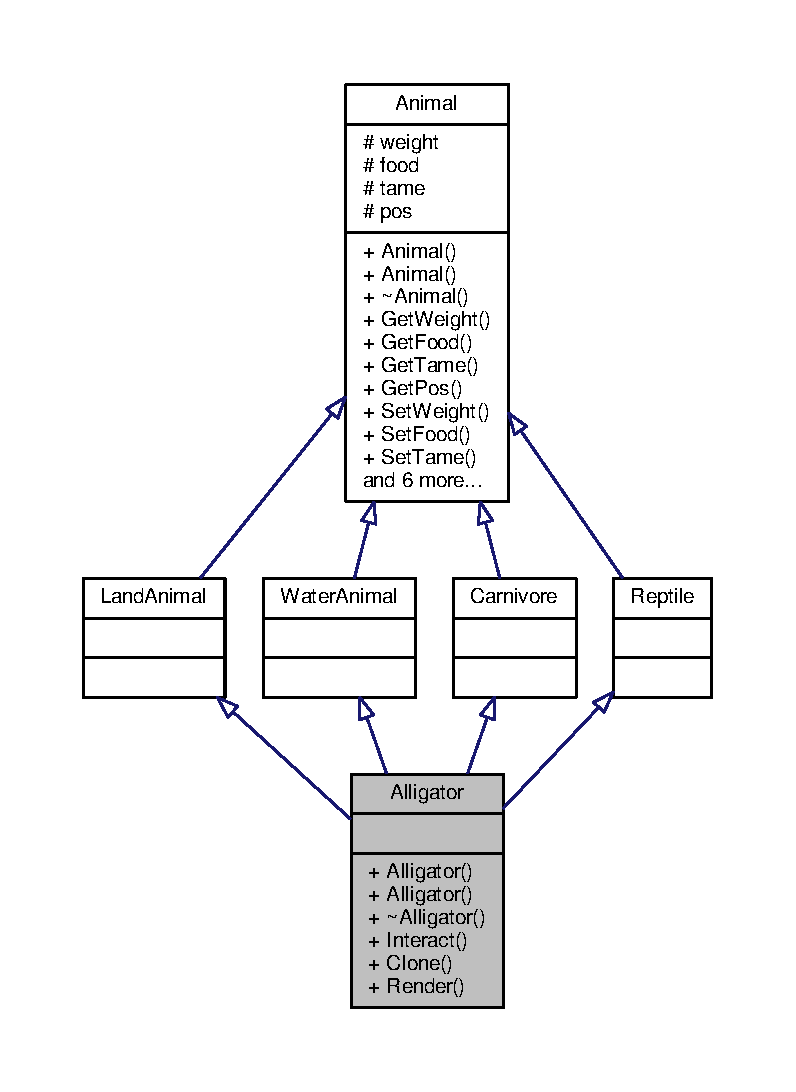
\includegraphics[width=218pt]{classAlligator__inherit__graph}
\end{center}
\end{figure}


Collaboration diagram for Alligator\+:
\nopagebreak
\begin{figure}[H]
\begin{center}
\leavevmode
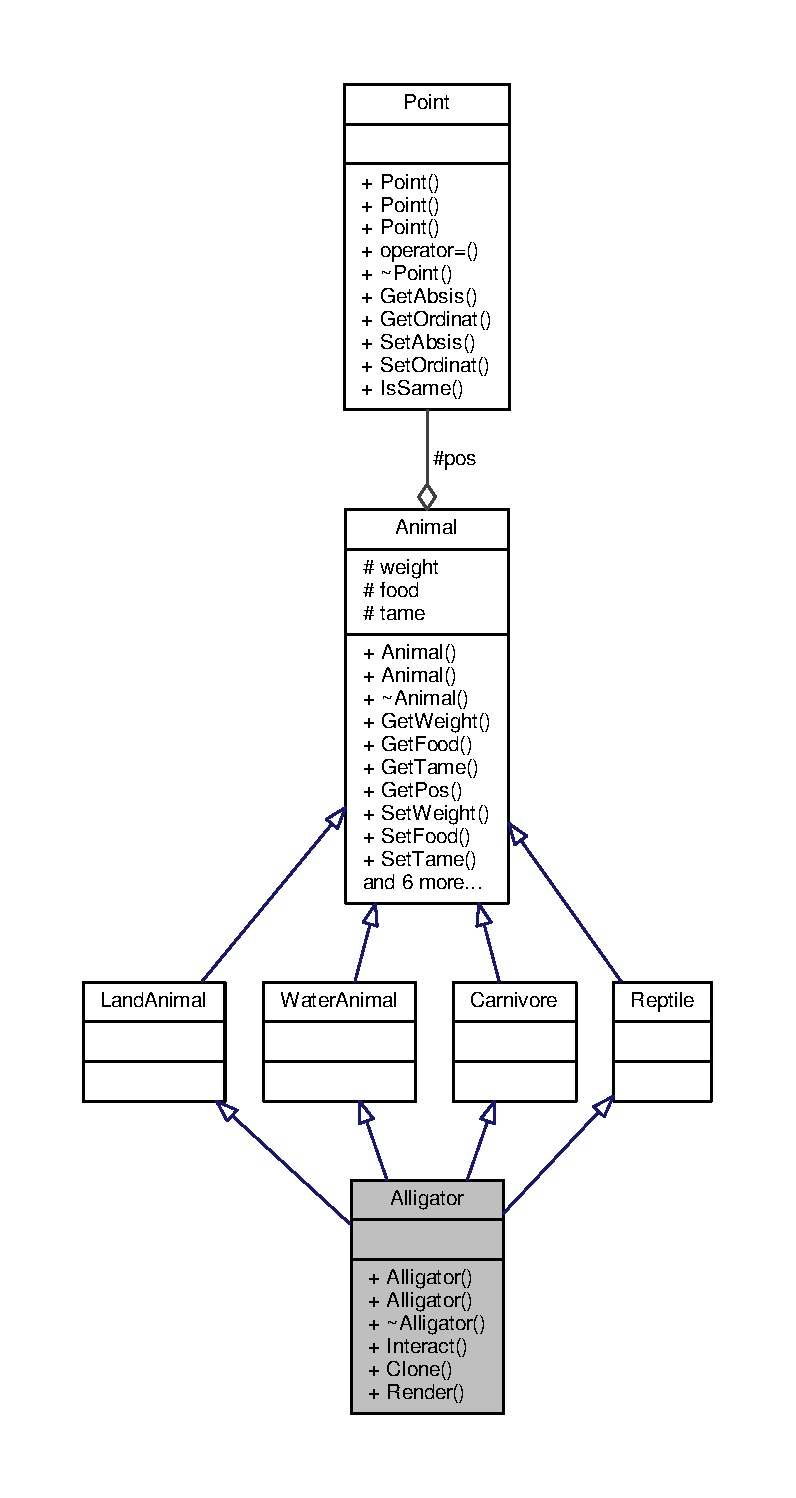
\includegraphics[height=550pt]{classAlligator__coll__graph}
\end{center}
\end{figure}
\subsection*{Public Member Functions}
\begin{DoxyCompactItemize}
\item 
\hyperlink{classAlligator_af1f21eea8d991b0ceb892448f456e587}{Alligator} ()
\begin{DoxyCompactList}\small\item\em Constructor. Menciptakan objek \hyperlink{classAlligator}{Alligator}. \end{DoxyCompactList}\item 
virtual \hyperlink{classAlligator_a9504f449fe1f01c94c0052f994340b14}{$\sim$\+Alligator} ()
\begin{DoxyCompactList}\small\item\em Destructor. \end{DoxyCompactList}\item 
string \hyperlink{classAlligator_a8f6141caa973d33f2066c3561cd817b3}{Interact} ()
\begin{DoxyCompactList}\small\item\em Interaksi yang dilakukan \hyperlink{classAlligator}{Alligator}. \end{DoxyCompactList}\item 
virtual \hyperlink{classAlligator}{Alligator} $\ast$ \hyperlink{classAlligator_aa317f0d37332919f638128c41cd7b53f}{Clone} () const 
\begin{DoxyCompactList}\small\item\em Melakukan cloning untuk menciptakan objek \hyperlink{classAlligator}{Alligator} baru. \end{DoxyCompactList}\item 
char \hyperlink{classAlligator_aa8f0a207888bf7f682ebc6b57270dd33}{Render} ()
\begin{DoxyCompactList}\small\item\em Render dari \hyperlink{classAlligator}{Alligator}. \end{DoxyCompactList}\end{DoxyCompactItemize}
\subsection*{Additional Inherited Members}


\subsection{Detailed Description}
Kelas \hyperlink{classAlligator}{Alligator} merupakan kelas untuk real object \hyperlink{classAlligator}{Alligator} 

\subsection{Constructor \& Destructor Documentation}
\index{Alligator@{Alligator}!Alligator@{Alligator}}
\index{Alligator@{Alligator}!Alligator@{Alligator}}
\subsubsection[{\texorpdfstring{Alligator()}{Alligator()}}]{\setlength{\rightskip}{0pt plus 5cm}Alligator\+::\+Alligator (
\begin{DoxyParamCaption}
{}
\end{DoxyParamCaption}
)\hspace{0.3cm}{\ttfamily [inline]}}\hypertarget{classAlligator_af1f21eea8d991b0ceb892448f456e587}{}\label{classAlligator_af1f21eea8d991b0ceb892448f456e587}


Constructor. Menciptakan objek \hyperlink{classAlligator}{Alligator}. 

\index{Alligator@{Alligator}!````~Alligator@{$\sim$\+Alligator}}
\index{````~Alligator@{$\sim$\+Alligator}!Alligator@{Alligator}}
\subsubsection[{\texorpdfstring{$\sim$\+Alligator()}{~Alligator()}}]{\setlength{\rightskip}{0pt plus 5cm}virtual Alligator\+::$\sim$\+Alligator (
\begin{DoxyParamCaption}
{}
\end{DoxyParamCaption}
)\hspace{0.3cm}{\ttfamily [inline]}, {\ttfamily [virtual]}}\hypertarget{classAlligator_a9504f449fe1f01c94c0052f994340b14}{}\label{classAlligator_a9504f449fe1f01c94c0052f994340b14}


Destructor. 



\subsection{Member Function Documentation}
\index{Alligator@{Alligator}!Clone@{Clone}}
\index{Clone@{Clone}!Alligator@{Alligator}}
\subsubsection[{\texorpdfstring{Clone() const }{Clone() const }}]{\setlength{\rightskip}{0pt plus 5cm}virtual {\bf Alligator}$\ast$ Alligator\+::\+Clone (
\begin{DoxyParamCaption}
{}
\end{DoxyParamCaption}
) const\hspace{0.3cm}{\ttfamily [inline]}, {\ttfamily [virtual]}}\hypertarget{classAlligator_aa317f0d37332919f638128c41cd7b53f}{}\label{classAlligator_aa317f0d37332919f638128c41cd7b53f}


Melakukan cloning untuk menciptakan objek \hyperlink{classAlligator}{Alligator} baru. 

\begin{DoxyReturn}{Returns}
Mengembalikan pointer to \hyperlink{classAlligator}{Alligator} objek tersebut. 
\end{DoxyReturn}


Implements \hyperlink{classAnimal_a3fc95e2a588b653b9b315e6c7a29c89f}{Animal}.

\index{Alligator@{Alligator}!Interact@{Interact}}
\index{Interact@{Interact}!Alligator@{Alligator}}
\subsubsection[{\texorpdfstring{Interact()}{Interact()}}]{\setlength{\rightskip}{0pt plus 5cm}string Alligator\+::\+Interact (
\begin{DoxyParamCaption}
{}
\end{DoxyParamCaption}
)\hspace{0.3cm}{\ttfamily [inline]}, {\ttfamily [virtual]}}\hypertarget{classAlligator_a8f6141caa973d33f2066c3561cd817b3}{}\label{classAlligator_a8f6141caa973d33f2066c3561cd817b3}


Interaksi yang dilakukan \hyperlink{classAlligator}{Alligator}. 

\begin{DoxyReturn}{Returns}
Mengembalikan string yang merepresentasikan suara \hyperlink{classAlligator}{Alligator}. 
\end{DoxyReturn}


Implements \hyperlink{classAnimal_ad5a55fb0355a9425fee6611003d9892c}{Animal}.

\index{Alligator@{Alligator}!Render@{Render}}
\index{Render@{Render}!Alligator@{Alligator}}
\subsubsection[{\texorpdfstring{Render()}{Render()}}]{\setlength{\rightskip}{0pt plus 5cm}char Alligator\+::\+Render (
\begin{DoxyParamCaption}
{}
\end{DoxyParamCaption}
)\hspace{0.3cm}{\ttfamily [inline]}, {\ttfamily [virtual]}}\hypertarget{classAlligator_aa8f0a207888bf7f682ebc6b57270dd33}{}\label{classAlligator_aa8f0a207888bf7f682ebc6b57270dd33}


Render dari \hyperlink{classAlligator}{Alligator}. 

\begin{DoxyReturn}{Returns}
Mengembalikan char yang merupakan representasi kode \hyperlink{classAlligator}{Alligator}. 
\end{DoxyReturn}


Implements \hyperlink{classAnimal_a43a47c0f41d211128e04abc6add53def}{Animal}.



The documentation for this class was generated from the following file\+:\begin{DoxyCompactItemize}
\item 
alligator/\hyperlink{alligator_8h}{alligator.\+h}\end{DoxyCompactItemize}

\hypertarget{classAnimal}{}\section{Animal Class Reference}
\label{classAnimal}\index{Animal@{Animal}}


{\ttfamily \#include $<$animal.\+h$>$}



Inheritance diagram for Animal\+:
\nopagebreak
\begin{figure}[H]
\begin{center}
\leavevmode
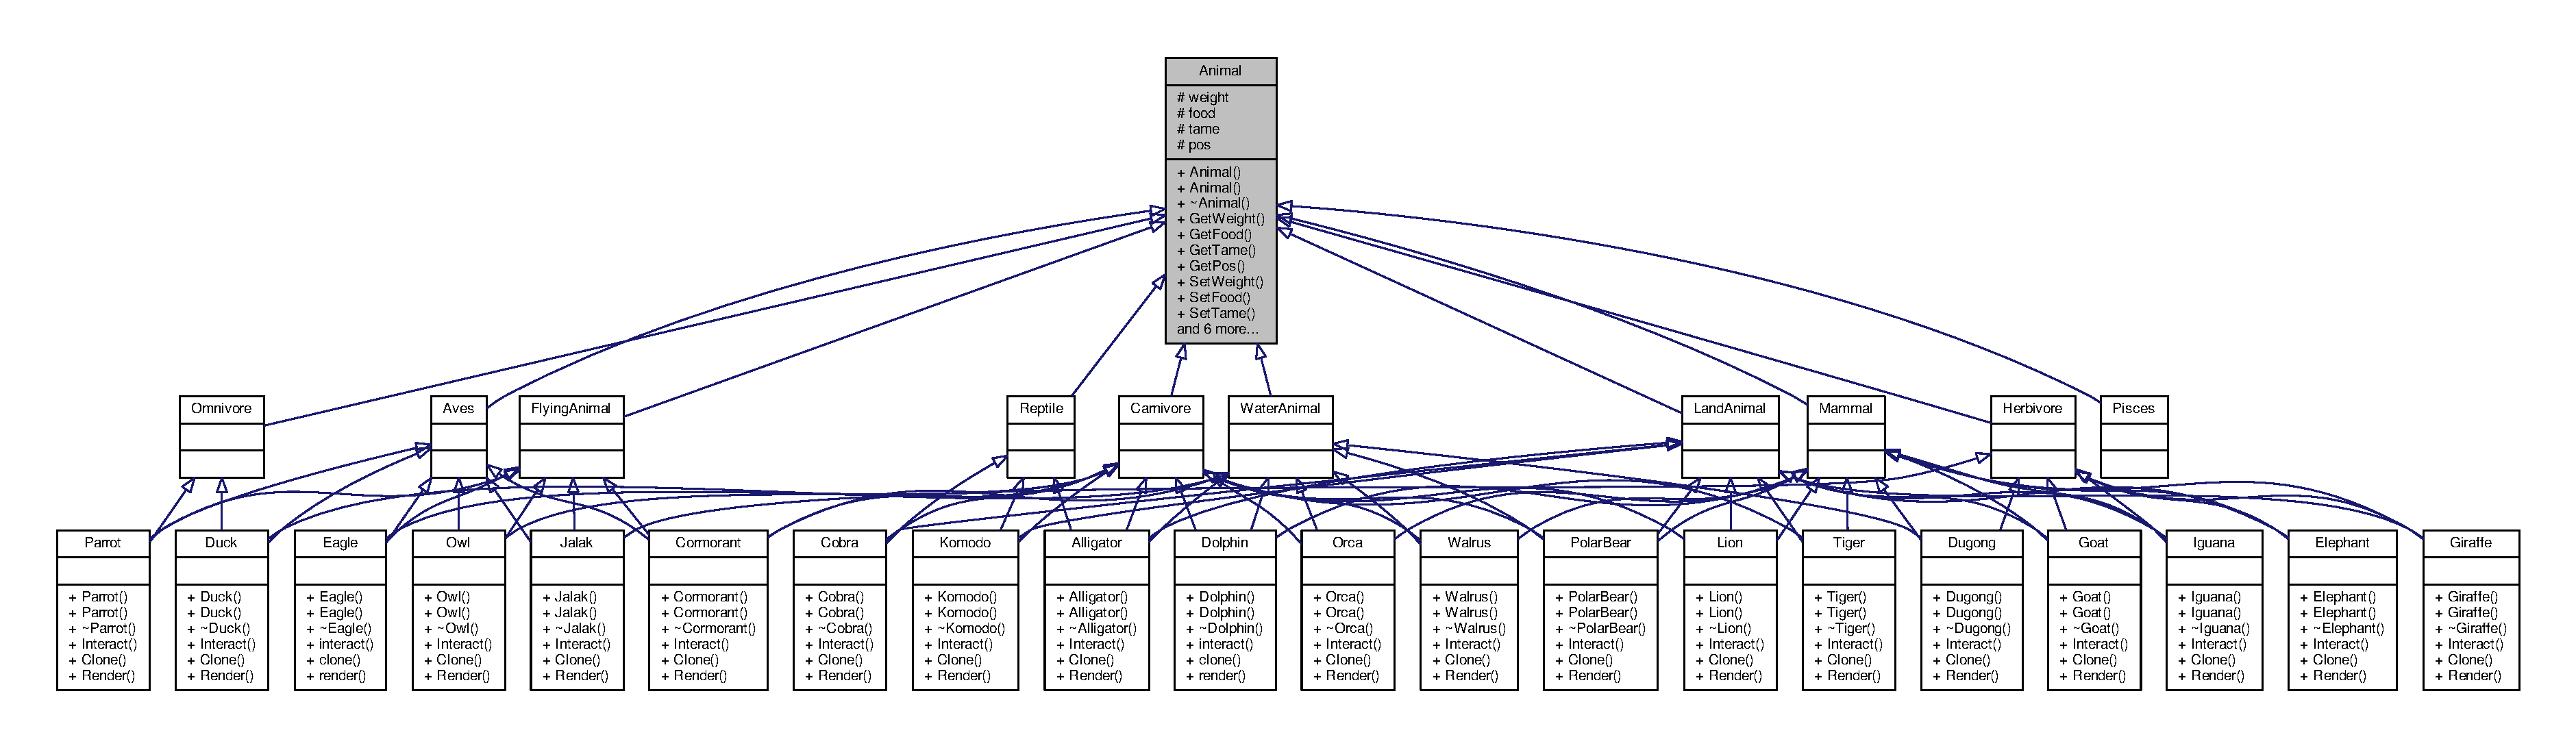
\includegraphics[width=350pt]{classAnimal__inherit__graph}
\end{center}
\end{figure}


Collaboration diagram for Animal\+:
\nopagebreak
\begin{figure}[H]
\begin{center}
\leavevmode
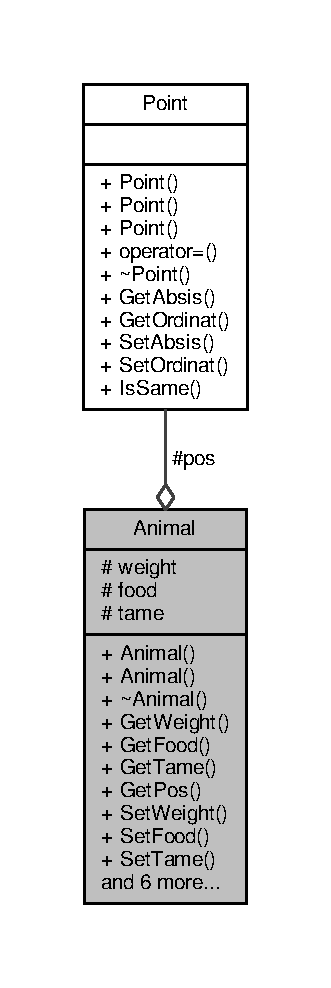
\includegraphics[width=159pt]{classAnimal__coll__graph}
\end{center}
\end{figure}
\subsection*{Public Member Functions}
\begin{DoxyCompactItemize}
\item 
\hyperlink{classAnimal_a1e726a49ec952443190ac62dad22353c}{Animal} ()
\begin{DoxyCompactList}\small\item\em Constructor. Menciptakan \hyperlink{classAnimal}{Animal} kosong. \end{DoxyCompactList}\item 
virtual \hyperlink{classAnimal_a16d8b7f94611cc65f5cdb58cc105527b}{$\sim$\+Animal} ()
\begin{DoxyCompactList}\small\item\em Destructor. \end{DoxyCompactList}\item 
\hyperlink{classPoint}{Point} \hyperlink{classAnimal_a183e4addbbccbe06a77e57bc8893cec1}{Get\+Pos} () const 
\begin{DoxyCompactList}\small\item\em Getter untuk pos. \end{DoxyCompactList}\item 
void \hyperlink{classAnimal_a754c7eb7a8ca6d8bd3e30650546a410d}{Set\+Point} (int abs, int ord)
\begin{DoxyCompactList}\small\item\em Setter point dengan parameter dua buah nilai integer. \end{DoxyCompactList}\item 
void \hyperlink{classAnimal_a02e187a6407bc83c46698544c912be15}{Set\+Point} (const \hyperlink{classPoint}{Point} \&p)
\begin{DoxyCompactList}\small\item\em Setter point dengan parameter sebuah point. \end{DoxyCompactList}\item 
bool \hyperlink{classAnimal_afc66abcbc6efb71c81d5306ea368cffb}{Is\+Same} (const \hyperlink{classAnimal}{Animal} \&a) const 
\begin{DoxyCompactList}\small\item\em Memeriksa kesamaan dua animal. \end{DoxyCompactList}\item 
virtual string \hyperlink{classAnimal_ad5a55fb0355a9425fee6611003d9892c}{Interact} ()=0
\begin{DoxyCompactList}\small\item\em Interaksi yang dilakukan animal. \end{DoxyCompactList}\item 
virtual \hyperlink{classAnimal}{Animal} $\ast$ \hyperlink{classAnimal_a3fc95e2a588b653b9b315e6c7a29c89f}{Clone} () const =0
\begin{DoxyCompactList}\small\item\em Melakukan cloning untuk menciptakan objek \hyperlink{classAnimal}{Animal} baru. \end{DoxyCompactList}\item 
virtual char \hyperlink{classAnimal_a43a47c0f41d211128e04abc6add53def}{Render} ()=0
\begin{DoxyCompactList}\small\item\em Render dari \hyperlink{classAnimal}{Animal}. \end{DoxyCompactList}\end{DoxyCompactItemize}
\subsection*{Protected Attributes}
\begin{DoxyCompactItemize}
\item 
\hyperlink{classPoint}{Point} \hyperlink{classAnimal_ae4e9a6fe53c7ebfbb00536f0e38de5c8}{pos}
\begin{DoxyCompactList}\small\item\em Lokasi binatang. \end{DoxyCompactList}\end{DoxyCompactItemize}


\subsection{Detailed Description}
Kelas abstrak \hyperlink{classAnimal}{Animal} merepresentasikan binatang dalam Virtual \hyperlink{classZoo}{Zoo} 

\subsection{Constructor \& Destructor Documentation}
\index{Animal@{Animal}!Animal@{Animal}}
\index{Animal@{Animal}!Animal@{Animal}}
\subsubsection[{\texorpdfstring{Animal()}{Animal()}}]{\setlength{\rightskip}{0pt plus 5cm}Animal\+::\+Animal (
\begin{DoxyParamCaption}
{}
\end{DoxyParamCaption}
)}\hypertarget{classAnimal_a1e726a49ec952443190ac62dad22353c}{}\label{classAnimal_a1e726a49ec952443190ac62dad22353c}


Constructor. Menciptakan \hyperlink{classAnimal}{Animal} kosong. 

\index{Animal@{Animal}!````~Animal@{$\sim$\+Animal}}
\index{````~Animal@{$\sim$\+Animal}!Animal@{Animal}}
\subsubsection[{\texorpdfstring{$\sim$\+Animal()}{~Animal()}}]{\setlength{\rightskip}{0pt plus 5cm}virtual Animal\+::$\sim$\+Animal (
\begin{DoxyParamCaption}
{}
\end{DoxyParamCaption}
)\hspace{0.3cm}{\ttfamily [inline]}, {\ttfamily [virtual]}}\hypertarget{classAnimal_a16d8b7f94611cc65f5cdb58cc105527b}{}\label{classAnimal_a16d8b7f94611cc65f5cdb58cc105527b}


Destructor. 



\subsection{Member Function Documentation}
\index{Animal@{Animal}!Clone@{Clone}}
\index{Clone@{Clone}!Animal@{Animal}}
\subsubsection[{\texorpdfstring{Clone() const =0}{Clone() const =0}}]{\setlength{\rightskip}{0pt plus 5cm}virtual {\bf Animal}$\ast$ Animal\+::\+Clone (
\begin{DoxyParamCaption}
{}
\end{DoxyParamCaption}
) const\hspace{0.3cm}{\ttfamily [pure virtual]}}\hypertarget{classAnimal_a3fc95e2a588b653b9b315e6c7a29c89f}{}\label{classAnimal_a3fc95e2a588b653b9b315e6c7a29c89f}


Melakukan cloning untuk menciptakan objek \hyperlink{classAnimal}{Animal} baru. 

\begin{DoxyReturn}{Returns}
Mengembalikan pointer to \hyperlink{classAnimal}{Animal} objek tersebut. 
\end{DoxyReturn}


Implemented in \hyperlink{classAlligator_aa317f0d37332919f638128c41cd7b53f}{Alligator}, \hyperlink{classCobra_a1bfd2035a0a700b6362b1853cb12949b}{Cobra}, \hyperlink{classCormorant_a7be371562fab8ab5c2e9e72386ee9aa2}{Cormorant}, \hyperlink{classDolphin_a4be3892432206693d2fae815303e07c4}{Dolphin}, \hyperlink{classDuck_ae3ff98b443c887f37ce63e3ed2e3a690}{Duck}, \hyperlink{classDugong_a8209b4208bd32dfc0fa4e701679306c1}{Dugong}, \hyperlink{classEagle_ace8cb419354688615938d2a53d5c1566}{Eagle}, \hyperlink{classElephant_a723a7c90f44a95d9886163e605aecea7}{Elephant}, \hyperlink{classGiraffe_aa29f8f77477a64fc72f814b7f225c94f}{Giraffe}, \hyperlink{classGoat_a1532200ef20734bb42d0a1306b14d8ad}{Goat}, \hyperlink{classIguana_a40e56fb855d09d2a8788dc73e2fdfc8a}{Iguana}, \hyperlink{classJalak_a85b145221386cdca75274b4438250161}{Jalak}, \hyperlink{classKomodo_aab3bd7ee8235c87e8bbafd8848968be8}{Komodo}, \hyperlink{classLion_ae63405ef106650644a8fcafc7393284e}{Lion}, \hyperlink{classOrca_ac44eb30486ba4051eefa914dc8cd670f}{Orca}, \hyperlink{classOwl_a585e73d53d76b2db489613b7f0b6eecc}{Owl}, \hyperlink{classParrot_aec7fd1385827d67522e1baf3242078b0}{Parrot}, \hyperlink{classPolarBear_aad58cdb9b360996a94f12ade5b6743b7}{Polar\+Bear}, \hyperlink{classTiger_aa376d57a4b2d56edb586f7ba1b170037}{Tiger}, and \hyperlink{classWalrus_a9644eb3d51eb945b716bd37e25c7470e}{Walrus}.

\index{Animal@{Animal}!Get\+Pos@{Get\+Pos}}
\index{Get\+Pos@{Get\+Pos}!Animal@{Animal}}
\subsubsection[{\texorpdfstring{Get\+Pos() const }{GetPos() const }}]{\setlength{\rightskip}{0pt plus 5cm}{\bf Point} Animal\+::\+Get\+Pos (
\begin{DoxyParamCaption}
{}
\end{DoxyParamCaption}
) const}\hypertarget{classAnimal_a183e4addbbccbe06a77e57bc8893cec1}{}\label{classAnimal_a183e4addbbccbe06a77e57bc8893cec1}


Getter untuk pos. 

\begin{DoxyReturn}{Returns}
Mengembalikan nilai lokasi binatang. 
\end{DoxyReturn}
\index{Animal@{Animal}!Interact@{Interact}}
\index{Interact@{Interact}!Animal@{Animal}}
\subsubsection[{\texorpdfstring{Interact()=0}{Interact()=0}}]{\setlength{\rightskip}{0pt plus 5cm}virtual string Animal\+::\+Interact (
\begin{DoxyParamCaption}
{}
\end{DoxyParamCaption}
)\hspace{0.3cm}{\ttfamily [pure virtual]}}\hypertarget{classAnimal_ad5a55fb0355a9425fee6611003d9892c}{}\label{classAnimal_ad5a55fb0355a9425fee6611003d9892c}


Interaksi yang dilakukan animal. 

\begin{DoxyReturn}{Returns}
Mengembalikan string yang merepresentasikan suara \hyperlink{classAnimal}{Animal}. 
\end{DoxyReturn}


Implemented in \hyperlink{classAlligator_a8f6141caa973d33f2066c3561cd817b3}{Alligator}, \hyperlink{classCobra_aa8dd0878e3d654e51bec9592c88bcab5}{Cobra}, \hyperlink{classCormorant_af28984652ae999452d20aed885f0185a}{Cormorant}, \hyperlink{classDolphin_a592506c38c185d7d383ae755deb9bd72}{Dolphin}, \hyperlink{classDuck_a9355aa821755703c02ac96e49692eaea}{Duck}, \hyperlink{classDugong_a861c589c05a791faf03297eb6e718d9e}{Dugong}, \hyperlink{classEagle_a64abae4f80bcdcba7dac9f03126f42aa}{Eagle}, \hyperlink{classElephant_a4f2c4bef5ec886019ee88ad575f94fa7}{Elephant}, \hyperlink{classGiraffe_ad73e5ee5fc62f709c52a1cab68f2a1f3}{Giraffe}, \hyperlink{classGoat_a5f480d88c50724cee8c7a9d18f486144}{Goat}, \hyperlink{classIguana_a271ef320fd3d4973e50e89aa30cffe3e}{Iguana}, \hyperlink{classJalak_a864b931f04f1580759c4a108e1734bb8}{Jalak}, \hyperlink{classKomodo_a250e6b06c369a94faaa551751cd09196}{Komodo}, \hyperlink{classLion_a4c090a9b5f42b92c30d223b40435e167}{Lion}, \hyperlink{classOrca_adf95ca04578ac04aaa717ef2dd11bf4c}{Orca}, \hyperlink{classOwl_ac3c735f8a34b46780a0efd052319e7f3}{Owl}, \hyperlink{classParrot_a3fdf1aa0851d53d31b5d225d755e4995}{Parrot}, \hyperlink{classPolarBear_a2c266e69dd929ac3b10fe7484a77a5a4}{Polar\+Bear}, \hyperlink{classTiger_ae318cc373300a52e13598f42368a2c70}{Tiger}, and \hyperlink{classWalrus_aa21a90ecf8aff97c4cf90a59449ce02c}{Walrus}.

\index{Animal@{Animal}!Is\+Same@{Is\+Same}}
\index{Is\+Same@{Is\+Same}!Animal@{Animal}}
\subsubsection[{\texorpdfstring{Is\+Same(const Animal \&a) const }{IsSame(const Animal &a) const }}]{\setlength{\rightskip}{0pt plus 5cm}bool Animal\+::\+Is\+Same (
\begin{DoxyParamCaption}
\item[{const {\bf Animal} \&}]{a}
\end{DoxyParamCaption}
) const}\hypertarget{classAnimal_afc66abcbc6efb71c81d5306ea368cffb}{}\label{classAnimal_afc66abcbc6efb71c81d5306ea368cffb}


Memeriksa kesamaan dua animal. 


\begin{DoxyParams}{Parameters}
{\em a} & Objek animal yang akan dibandingkan. \\
\hline
\end{DoxyParams}
\begin{DoxyReturn}{Returns}
Mengeluarkan true jika current object sama dengan animal a. 
\end{DoxyReturn}
\index{Animal@{Animal}!Render@{Render}}
\index{Render@{Render}!Animal@{Animal}}
\subsubsection[{\texorpdfstring{Render()=0}{Render()=0}}]{\setlength{\rightskip}{0pt plus 5cm}virtual char Animal\+::\+Render (
\begin{DoxyParamCaption}
{}
\end{DoxyParamCaption}
)\hspace{0.3cm}{\ttfamily [pure virtual]}}\hypertarget{classAnimal_a43a47c0f41d211128e04abc6add53def}{}\label{classAnimal_a43a47c0f41d211128e04abc6add53def}


Render dari \hyperlink{classAnimal}{Animal}. 

\begin{DoxyReturn}{Returns}
Mengembalikan char yang merupakan representasi kode \hyperlink{classAnimal}{Animal}. 
\end{DoxyReturn}


Implemented in \hyperlink{classAlligator_aa8f0a207888bf7f682ebc6b57270dd33}{Alligator}, \hyperlink{classCobra_abca7da2ee55ce825dc49f4f9a3e87208}{Cobra}, \hyperlink{classCormorant_a6d388885acfc98de6020a01b90259dac}{Cormorant}, \hyperlink{classDolphin_aa051d8ebe93c1c11b503ae76d07cd178}{Dolphin}, \hyperlink{classDuck_a8453f95adcf2e7ff1b35a1a9d9948510}{Duck}, \hyperlink{classDugong_af82a8983c960604aa27dabe7fec53362}{Dugong}, \hyperlink{classEagle_a34e512cb19b5ba1f8a7bce937c57f33f}{Eagle}, \hyperlink{classElephant_a7e412f36e1f88cd278dea76d4f383e95}{Elephant}, \hyperlink{classGiraffe_a64dccf030fdb54de9fd37f8381c64271}{Giraffe}, \hyperlink{classGoat_aedea4680fe17571c2f51d35b90397f6e}{Goat}, \hyperlink{classIguana_a18bbb71a80e6b2a9855623b1c7f108b9}{Iguana}, \hyperlink{classJalak_af500189104401b66d6ab4e3b1106ce74}{Jalak}, \hyperlink{classKomodo_a06ce8ed3d58a33968ecf4a12a3ebbd4d}{Komodo}, \hyperlink{classLion_ad782de7c88e4a7aad01287a2ed64827c}{Lion}, \hyperlink{classOrca_a0673bfc8e70af67b463a4fcae224d9d5}{Orca}, \hyperlink{classOwl_ab4ecc1fc8da822f97299709508f7806d}{Owl}, \hyperlink{classParrot_a27c491ab4ae56491fbe8d74e494bc46d}{Parrot}, \hyperlink{classPolarBear_a7feccf8999fb0ab000c052583ad0217a}{Polar\+Bear}, \hyperlink{classTiger_a42b09a0bfc8c115e7383e926513fb371}{Tiger}, and \hyperlink{classWalrus_a143f948e4c45e13a67f893caa435475d}{Walrus}.

\index{Animal@{Animal}!Set\+Point@{Set\+Point}}
\index{Set\+Point@{Set\+Point}!Animal@{Animal}}
\subsubsection[{\texorpdfstring{Set\+Point(int abs, int ord)}{SetPoint(int abs, int ord)}}]{\setlength{\rightskip}{0pt plus 5cm}void Animal\+::\+Set\+Point (
\begin{DoxyParamCaption}
\item[{int}]{abs, }
\item[{int}]{ord}
\end{DoxyParamCaption}
)}\hypertarget{classAnimal_a754c7eb7a8ca6d8bd3e30650546a410d}{}\label{classAnimal_a754c7eb7a8ca6d8bd3e30650546a410d}


Setter point dengan parameter dua buah nilai integer. 


\begin{DoxyParams}{Parameters}
{\em abs} & Nilai absis yang akan di-\/set pada lokasi animal. \\
\hline
{\em ord} & Nilai ordinat yang akan di-\/set pada lokasi animal. \\
\hline
\end{DoxyParams}
\index{Animal@{Animal}!Set\+Point@{Set\+Point}}
\index{Set\+Point@{Set\+Point}!Animal@{Animal}}
\subsubsection[{\texorpdfstring{Set\+Point(const Point \&p)}{SetPoint(const Point &p)}}]{\setlength{\rightskip}{0pt plus 5cm}void Animal\+::\+Set\+Point (
\begin{DoxyParamCaption}
\item[{const {\bf Point} \&}]{p}
\end{DoxyParamCaption}
)}\hypertarget{classAnimal_a02e187a6407bc83c46698544c912be15}{}\label{classAnimal_a02e187a6407bc83c46698544c912be15}


Setter point dengan parameter sebuah point. 


\begin{DoxyParams}{Parameters}
{\em p} & Objek point yang akan di-\/set pada lokasi animal. \\
\hline
\end{DoxyParams}


\subsection{Member Data Documentation}
\index{Animal@{Animal}!pos@{pos}}
\index{pos@{pos}!Animal@{Animal}}
\subsubsection[{\texorpdfstring{pos}{pos}}]{\setlength{\rightskip}{0pt plus 5cm}{\bf Point} Animal\+::pos\hspace{0.3cm}{\ttfamily [protected]}}\hypertarget{classAnimal_ae4e9a6fe53c7ebfbb00536f0e38de5c8}{}\label{classAnimal_ae4e9a6fe53c7ebfbb00536f0e38de5c8}


Lokasi binatang. 



The documentation for this class was generated from the following files\+:\begin{DoxyCompactItemize}
\item 
animal/\hyperlink{animal_8h}{animal.\+h}\item 
animal/\hyperlink{animal_8cpp}{animal.\+cpp}\end{DoxyCompactItemize}

\hypertarget{classAves}{}\section{Aves Class Reference}
\label{classAves}\index{Aves@{Aves}}


{\ttfamily \#include $<$aves.\+h$>$}



Inheritance diagram for Aves\+:
\nopagebreak
\begin{figure}[H]
\begin{center}
\leavevmode
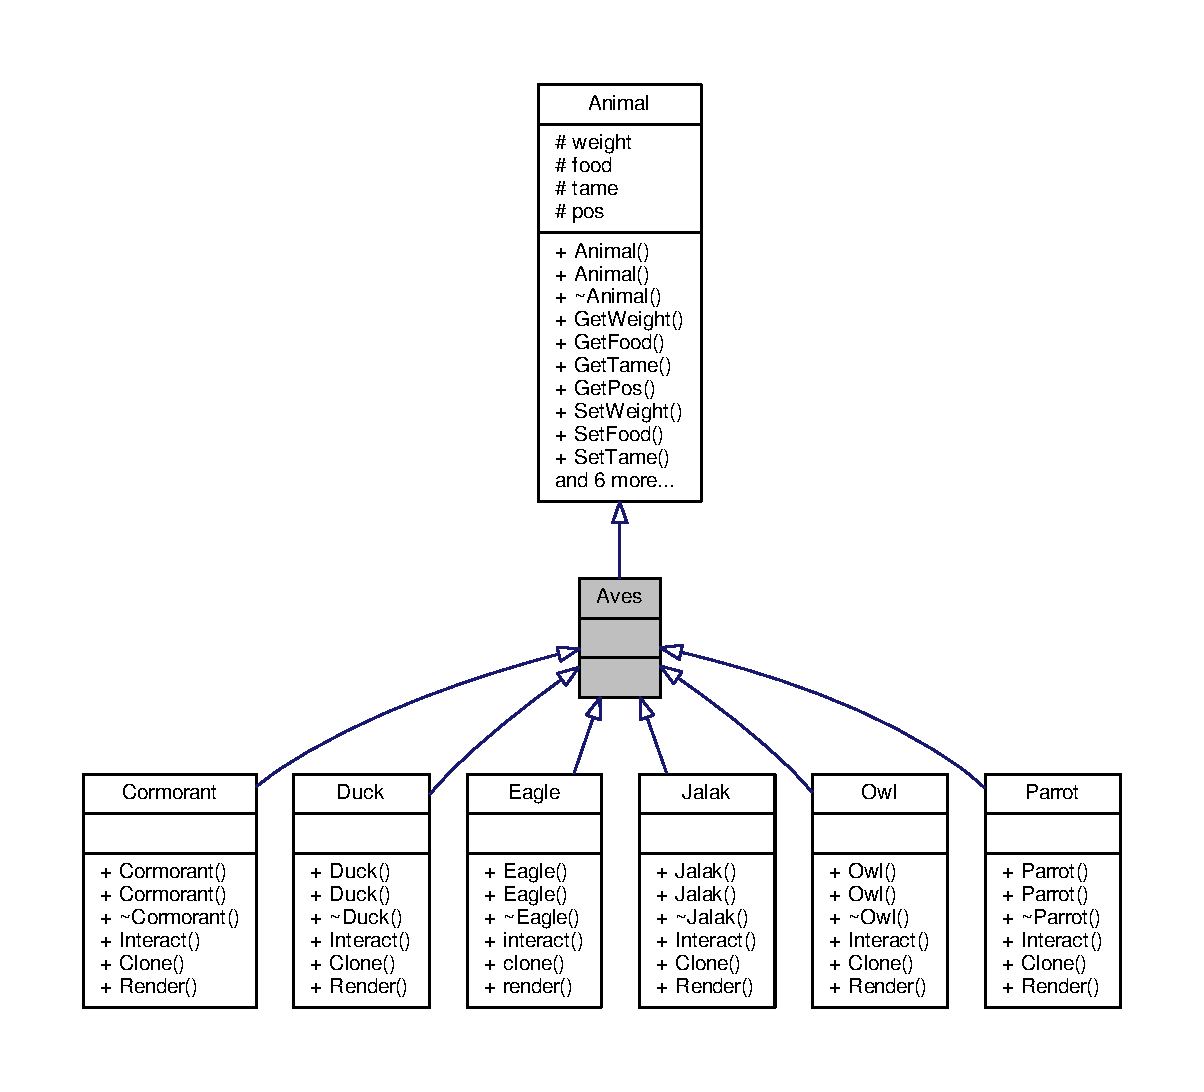
\includegraphics[width=350pt]{classAves__inherit__graph}
\end{center}
\end{figure}


Collaboration diagram for Aves\+:
\nopagebreak
\begin{figure}[H]
\begin{center}
\leavevmode
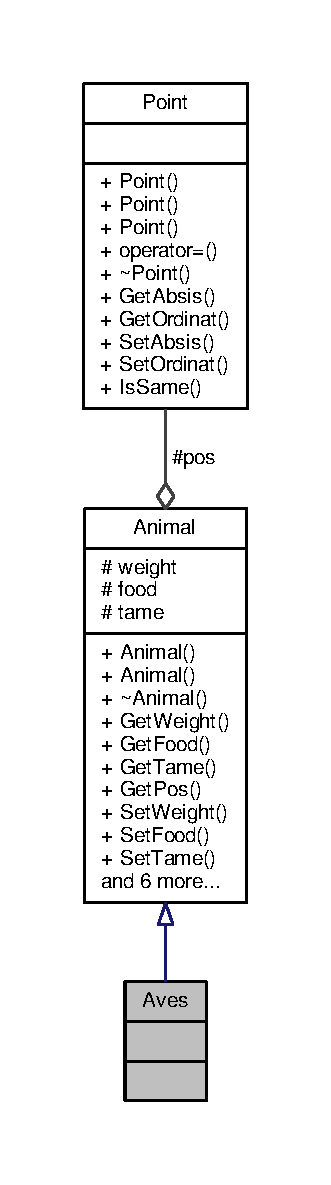
\includegraphics[height=550pt]{classAves__coll__graph}
\end{center}
\end{figure}
\subsection*{Additional Inherited Members}


\subsection{Detailed Description}
Kelas abstrak \hyperlink{classAves}{Aves} 

The documentation for this class was generated from the following file\+:\begin{DoxyCompactItemize}
\item 
aves/\hyperlink{aves_8h}{aves.\+h}\end{DoxyCompactItemize}

\hypertarget{classCage}{}\section{Cage Class Reference}
\label{classCage}\index{Cage@{Cage}}


{\ttfamily \#include $<$cage.\+h$>$}



Collaboration diagram for Cage\+:
% FIG 0
\subsection*{Classes}
\begin{DoxyCompactItemize}
\item 
class \hyperlink{classCage_1_1Kelas}{Kelas}
\end{DoxyCompactItemize}
\subsection*{Public Member Functions}
\begin{DoxyCompactItemize}
\item 
\hyperlink{classCage_ac03246dd263ee9fe6f37336317e62b69}{Cage} ()
\begin{DoxyCompactList}\small\item\em Constructor. Menciptakan \hyperlink{classCage}{Cage} kosong tanpa animal. \end{DoxyCompactList}\item 
\hyperlink{classCage_a8cd728b1eb23303888a153230f96490e}{Cage} (int s)
\begin{DoxyCompactList}\small\item\em Constructor dengan parameter. Menciptakan \hyperlink{classCage}{Cage} dengan size s tanpa animal. \end{DoxyCompactList}\item 
\hyperlink{classCage_a105ec044af346561cc7165f69da8cf08}{Cage} (int i, int j)
\begin{DoxyCompactList}\small\item\em Constructor. Menciptakan \hyperlink{classCage}{Cage} dengan size 1 dan loc i,j. \end{DoxyCompactList}\item 
\hyperlink{classCage_ae85bb53517616422bf7f36282de01519}{Cage} (const \hyperlink{classCage}{Cage} \&c)
\begin{DoxyCompactList}\small\item\em Copy Constructor. \end{DoxyCompactList}\item 
\hyperlink{classCage}{Cage} \& \hyperlink{classCage_a020eefd2b5d15915cf65693413be64db}{operator=} (const \hyperlink{classCage}{Cage} \&c)
\begin{DoxyCompactList}\small\item\em Operator =. \end{DoxyCompactList}\item 
\hyperlink{classCage_a657259499dfc23c63fc65aeaf8abbb17}{$\sim$\+Cage} ()
\begin{DoxyCompactList}\small\item\em Destructor. \end{DoxyCompactList}\item 
bool \hyperlink{classCage_af244dea5f1b3645d3f216a16f353ddc7}{Is\+Full} () const 
\begin{DoxyCompactList}\small\item\em Is\+Full. Menentukan apakah cage penuh. \end{DoxyCompactList}\item 
int \hyperlink{classCage_abf801136c687ea862b64d0c36a2ce5cd}{Get\+Size} () const 
\begin{DoxyCompactList}\small\item\em Get\+Size. \end{DoxyCompactList}\item 
\hyperlink{classAnimal}{Animal} \hyperlink{classCage_a298833379b741edbdaf5115e4993db1e}{Get\+Animal} (int i) const 
\begin{DoxyCompactList}\small\item\em Get\+Animal. \end{DoxyCompactList}\item 
int \hyperlink{classCage_a49312121ccca0c0b731f3fe1256a28a2}{Get\+Total\+Animal} () const 
\begin{DoxyCompactList}\small\item\em Get\+Total\+Animal. \end{DoxyCompactList}\item 
\hyperlink{classPoint}{Point} \hyperlink{classCage_ae01123979c931296ca477d9d15d9efba}{Get\+Point} (int i) const 
\begin{DoxyCompactList}\small\item\em Get\+Point. \end{DoxyCompactList}\item 
void \hyperlink{classCage_a928e4a1686c1c9ca4f7e703d107de415}{Adopt\+Animal} (\hyperlink{classAnimal}{Animal} A)
\begin{DoxyCompactList}\small\item\em Adopt\+Animal. \end{DoxyCompactList}\item 
void \hyperlink{classCage_a84c0aac0bfd315ef7e5d0595dea5be5a}{Release\+Animal} (int i)
\begin{DoxyCompactList}\small\item\em Release\+Animal. Melepas suatu binatang yang terdapat pada cage. \end{DoxyCompactList}\item 
bool \hyperlink{classCage_a8f2321f5ca7e5fed271350ea1800e10b}{Is\+Empty} () const 
\begin{DoxyCompactList}\small\item\em Is\+Empty. \end{DoxyCompactList}\item 
bool \hyperlink{classCage_aafb5de9009a7ef80fc039f27793c8df6}{Is\+Occupied} (int i) const 
\begin{DoxyCompactList}\small\item\em Is\+Occupied. Menentukan apakah \hyperlink{classCage}{Cage} sudah terisi. \end{DoxyCompactList}\item 
bool \hyperlink{classCage_a176fc9feeb9855881e85c5d8551a6443}{Is\+Occupied} (const \hyperlink{classPoint}{Point} \&p) const 
\begin{DoxyCompactList}\small\item\em Is\+Occupied. Menentukan apakah \hyperlink{classCage}{Cage} sudah terisi. \end{DoxyCompactList}\item 
int \hyperlink{classCage_aaf098729df55f3cf45068d32fe6d5c4b}{Is\+In\+Cage} (const \hyperlink{classAnimal}{Animal} \&A) const 
\begin{DoxyCompactList}\small\item\em Is\+In\+Cage. Menentukan apakah suatu binatang terdapat pada cage. \end{DoxyCompactList}\item 
bool \hyperlink{classCage_a2ac9ea442655213ae3d52a6a7dc30fcf}{Is\+In\+Cage} (const \hyperlink{classPoint}{Point} \&P) const 
\begin{DoxyCompactList}\small\item\em Is\+In\+Cage. Menentukan apakah P terdapat dalam cage. \end{DoxyCompactList}\item 
void \hyperlink{classCage_a78f919dc2b8a3e89a7375c97643a2633}{Interact} () const 
\begin{DoxyCompactList}\small\item\em Interact. Mencetak interaksi animal cage ke layar. \end{DoxyCompactList}\item 
void \hyperlink{classCage_aed8ca487fb22db2ca755bc9d784342fc}{Add\+Point} (\hyperlink{classPoint}{Point} P)
\begin{DoxyCompactList}\small\item\em Add\+Point. Menambahkan Loc baru di dalam \hyperlink{classCage}{Cage}. \end{DoxyCompactList}\item 
bool \hyperlink{classCage_aece0c17d0299b55c596eb68175df71a8}{Can\+Put} (const \hyperlink{classAnimal}{Animal} \&A) const 
\begin{DoxyCompactList}\small\item\em Can\+Put. Menentukan apakah A dapat dimasukkan ke cage. \end{DoxyCompactList}\item 
bool \hyperlink{classCage_a973611397e576888027012237486cd25}{Move} ()
\begin{DoxyCompactList}\small\item\em Move. Menggerakkan semua binatang yang terdapat pada cage. \end{DoxyCompactList}\end{DoxyCompactItemize}


\subsection{Constructor \& Destructor Documentation}
\index{Cage@{Cage}!Cage@{Cage}}
\index{Cage@{Cage}!Cage@{Cage}}
\subsubsection[{\texorpdfstring{Cage()}{Cage()}}]{\setlength{\rightskip}{0pt plus 5cm}Cage\+::\+Cage (
\begin{DoxyParamCaption}
{}
\end{DoxyParamCaption}
)}\hypertarget{classCage_ac03246dd263ee9fe6f37336317e62b69}{}\label{classCage_ac03246dd263ee9fe6f37336317e62b69}


Constructor. Menciptakan \hyperlink{classCage}{Cage} kosong tanpa animal. 

\index{Cage@{Cage}!Cage@{Cage}}
\index{Cage@{Cage}!Cage@{Cage}}
\subsubsection[{\texorpdfstring{Cage(int s)}{Cage(int s)}}]{\setlength{\rightskip}{0pt plus 5cm}Cage\+::\+Cage (
\begin{DoxyParamCaption}
\item[{int}]{s}
\end{DoxyParamCaption}
)}\hypertarget{classCage_a8cd728b1eb23303888a153230f96490e}{}\label{classCage_a8cd728b1eb23303888a153230f96490e}


Constructor dengan parameter. Menciptakan \hyperlink{classCage}{Cage} dengan size s tanpa animal. 


\begin{DoxyParams}{Parameters}
{\em s} & Nilai ukuran \hyperlink{classCage}{Cage}. \\
\hline
\end{DoxyParams}
\index{Cage@{Cage}!Cage@{Cage}}
\index{Cage@{Cage}!Cage@{Cage}}
\subsubsection[{\texorpdfstring{Cage(int i, int j)}{Cage(int i, int j)}}]{\setlength{\rightskip}{0pt plus 5cm}Cage\+::\+Cage (
\begin{DoxyParamCaption}
\item[{int}]{i, }
\item[{int}]{j}
\end{DoxyParamCaption}
)}\hypertarget{classCage_a105ec044af346561cc7165f69da8cf08}{}\label{classCage_a105ec044af346561cc7165f69da8cf08}


Constructor. Menciptakan \hyperlink{classCage}{Cage} dengan size 1 dan loc i,j. 


\begin{DoxyParams}{Parameters}
{\em i} & absis \hyperlink{classPoint}{Point} pada \hyperlink{classCage}{Cage}. \\
\hline
{\em j} & ordinat \hyperlink{classPoint}{Point} pada \hyperlink{classCage}{Cage}. \\
\hline
\end{DoxyParams}
\index{Cage@{Cage}!Cage@{Cage}}
\index{Cage@{Cage}!Cage@{Cage}}
\subsubsection[{\texorpdfstring{Cage(const Cage \&c)}{Cage(const Cage &c)}}]{\setlength{\rightskip}{0pt plus 5cm}Cage\+::\+Cage (
\begin{DoxyParamCaption}
\item[{const {\bf Cage} \&}]{c}
\end{DoxyParamCaption}
)}\hypertarget{classCage_ae85bb53517616422bf7f36282de01519}{}\label{classCage_ae85bb53517616422bf7f36282de01519}


Copy Constructor. 


\begin{DoxyParams}{Parameters}
{\em c} & Objek yang akan di-\/copy. \\
\hline
\end{DoxyParams}
\index{Cage@{Cage}!````~Cage@{$\sim$\+Cage}}
\index{````~Cage@{$\sim$\+Cage}!Cage@{Cage}}
\subsubsection[{\texorpdfstring{$\sim$\+Cage()}{~Cage()}}]{\setlength{\rightskip}{0pt plus 5cm}Cage\+::$\sim$\+Cage (
\begin{DoxyParamCaption}
{}
\end{DoxyParamCaption}
)}\hypertarget{classCage_a657259499dfc23c63fc65aeaf8abbb17}{}\label{classCage_a657259499dfc23c63fc65aeaf8abbb17}


Destructor. 



\subsection{Member Function Documentation}
\index{Cage@{Cage}!Add\+Point@{Add\+Point}}
\index{Add\+Point@{Add\+Point}!Cage@{Cage}}
\subsubsection[{\texorpdfstring{Add\+Point(\+Point P)}{AddPoint(Point P)}}]{\setlength{\rightskip}{0pt plus 5cm}void Cage\+::\+Add\+Point (
\begin{DoxyParamCaption}
\item[{{\bf Point}}]{P}
\end{DoxyParamCaption}
)}\hypertarget{classCage_aed8ca487fb22db2ca755bc9d784342fc}{}\label{classCage_aed8ca487fb22db2ca755bc9d784342fc}


Add\+Point. Menambahkan Loc baru di dalam \hyperlink{classCage}{Cage}. 

\index{Cage@{Cage}!Adopt\+Animal@{Adopt\+Animal}}
\index{Adopt\+Animal@{Adopt\+Animal}!Cage@{Cage}}
\subsubsection[{\texorpdfstring{Adopt\+Animal(\+Animal A)}{AdoptAnimal(Animal A)}}]{\setlength{\rightskip}{0pt plus 5cm}void Cage\+::\+Adopt\+Animal (
\begin{DoxyParamCaption}
\item[{{\bf Animal}}]{A}
\end{DoxyParamCaption}
)}\hypertarget{classCage_a928e4a1686c1c9ca4f7e703d107de415}{}\label{classCage_a928e4a1686c1c9ca4f7e703d107de415}


Adopt\+Animal. 


\begin{DoxyParams}{Parameters}
{\em A} & Objek binatang yang akan dimasukkan. \\
\hline
\end{DoxyParams}
\index{Cage@{Cage}!Can\+Put@{Can\+Put}}
\index{Can\+Put@{Can\+Put}!Cage@{Cage}}
\subsubsection[{\texorpdfstring{Can\+Put(const Animal \&\+A) const }{CanPut(const Animal &A) const }}]{\setlength{\rightskip}{0pt plus 5cm}bool Cage\+::\+Can\+Put (
\begin{DoxyParamCaption}
\item[{const {\bf Animal} \&}]{A}
\end{DoxyParamCaption}
) const}\hypertarget{classCage_aece0c17d0299b55c596eb68175df71a8}{}\label{classCage_aece0c17d0299b55c596eb68175df71a8}


Can\+Put. Menentukan apakah A dapat dimasukkan ke cage. 


\begin{DoxyParams}{Parameters}
{\em A} & \hyperlink{classAnimal}{Animal} yang akan dimasukkan. \\
\hline
\end{DoxyParams}
\begin{DoxyReturn}{Returns}
Mengeluarkan true jika A dapat dimasukkan ke cage. 
\end{DoxyReturn}
\index{Cage@{Cage}!Get\+Animal@{Get\+Animal}}
\index{Get\+Animal@{Get\+Animal}!Cage@{Cage}}
\subsubsection[{\texorpdfstring{Get\+Animal(int i) const }{GetAnimal(int i) const }}]{\setlength{\rightskip}{0pt plus 5cm}{\bf Animal} Cage\+::\+Get\+Animal (
\begin{DoxyParamCaption}
\item[{int}]{i}
\end{DoxyParamCaption}
) const\hspace{0.3cm}{\ttfamily [inline]}}\hypertarget{classCage_a298833379b741edbdaf5115e4993db1e}{}\label{classCage_a298833379b741edbdaf5115e4993db1e}


Get\+Animal. 

\begin{DoxyReturn}{Returns}
Mengembalikan array animal pada \hyperlink{classCage}{Cage}. 
\end{DoxyReturn}
\index{Cage@{Cage}!Get\+Point@{Get\+Point}}
\index{Get\+Point@{Get\+Point}!Cage@{Cage}}
\subsubsection[{\texorpdfstring{Get\+Point(int i) const }{GetPoint(int i) const }}]{\setlength{\rightskip}{0pt plus 5cm}{\bf Point} Cage\+::\+Get\+Point (
\begin{DoxyParamCaption}
\item[{int}]{i}
\end{DoxyParamCaption}
) const\hspace{0.3cm}{\ttfamily [inline]}}\hypertarget{classCage_ae01123979c931296ca477d9d15d9efba}{}\label{classCage_ae01123979c931296ca477d9d15d9efba}


Get\+Point. 


\begin{DoxyParams}{Parameters}
{\em i} & Nilai indeks yang akan diperiksa. \\
\hline
\end{DoxyParams}
\begin{DoxyReturn}{Returns}
Mengembalikan lokasi \hyperlink{classCage}{Cage} pada indeks i. 
\end{DoxyReturn}
\index{Cage@{Cage}!Get\+Size@{Get\+Size}}
\index{Get\+Size@{Get\+Size}!Cage@{Cage}}
\subsubsection[{\texorpdfstring{Get\+Size() const }{GetSize() const }}]{\setlength{\rightskip}{0pt plus 5cm}int Cage\+::\+Get\+Size (
\begin{DoxyParamCaption}
{}
\end{DoxyParamCaption}
) const\hspace{0.3cm}{\ttfamily [inline]}}\hypertarget{classCage_abf801136c687ea862b64d0c36a2ce5cd}{}\label{classCage_abf801136c687ea862b64d0c36a2ce5cd}


Get\+Size. 

\begin{DoxyReturn}{Returns}
Mengembalikan nilai ukuran \hyperlink{classCage}{Cage}. 
\end{DoxyReturn}
\index{Cage@{Cage}!Get\+Total\+Animal@{Get\+Total\+Animal}}
\index{Get\+Total\+Animal@{Get\+Total\+Animal}!Cage@{Cage}}
\subsubsection[{\texorpdfstring{Get\+Total\+Animal() const }{GetTotalAnimal() const }}]{\setlength{\rightskip}{0pt plus 5cm}int Cage\+::\+Get\+Total\+Animal (
\begin{DoxyParamCaption}
{}
\end{DoxyParamCaption}
) const\hspace{0.3cm}{\ttfamily [inline]}}\hypertarget{classCage_a49312121ccca0c0b731f3fe1256a28a2}{}\label{classCage_a49312121ccca0c0b731f3fe1256a28a2}


Get\+Total\+Animal. 

\begin{DoxyReturn}{Returns}
Mengembalikan jumlah binatang pada \hyperlink{classCage}{Cage}. 
\end{DoxyReturn}
\index{Cage@{Cage}!Interact@{Interact}}
\index{Interact@{Interact}!Cage@{Cage}}
\subsubsection[{\texorpdfstring{Interact() const }{Interact() const }}]{\setlength{\rightskip}{0pt plus 5cm}void Cage\+::\+Interact (
\begin{DoxyParamCaption}
{}
\end{DoxyParamCaption}
) const}\hypertarget{classCage_a78f919dc2b8a3e89a7375c97643a2633}{}\label{classCage_a78f919dc2b8a3e89a7375c97643a2633}


Interact. Mencetak interaksi animal cage ke layar. 

\index{Cage@{Cage}!Is\+Empty@{Is\+Empty}}
\index{Is\+Empty@{Is\+Empty}!Cage@{Cage}}
\subsubsection[{\texorpdfstring{Is\+Empty() const }{IsEmpty() const }}]{\setlength{\rightskip}{0pt plus 5cm}bool Cage\+::\+Is\+Empty (
\begin{DoxyParamCaption}
{}
\end{DoxyParamCaption}
) const\hspace{0.3cm}{\ttfamily [inline]}}\hypertarget{classCage_a8f2321f5ca7e5fed271350ea1800e10b}{}\label{classCage_a8f2321f5ca7e5fed271350ea1800e10b}


Is\+Empty. 

\begin{DoxyReturn}{Returns}
Menghasilkan true jika \hyperlink{classCage}{Cage} kosong. 
\end{DoxyReturn}
\index{Cage@{Cage}!Is\+Full@{Is\+Full}}
\index{Is\+Full@{Is\+Full}!Cage@{Cage}}
\subsubsection[{\texorpdfstring{Is\+Full() const }{IsFull() const }}]{\setlength{\rightskip}{0pt plus 5cm}bool Cage\+::\+Is\+Full (
\begin{DoxyParamCaption}
{}
\end{DoxyParamCaption}
) const\hspace{0.3cm}{\ttfamily [inline]}}\hypertarget{classCage_af244dea5f1b3645d3f216a16f353ddc7}{}\label{classCage_af244dea5f1b3645d3f216a16f353ddc7}


Is\+Full. Menentukan apakah cage penuh. 

\begin{DoxyReturn}{Returns}
Mengeluarkan true jika cage penuh. 
\end{DoxyReturn}
\index{Cage@{Cage}!Is\+In\+Cage@{Is\+In\+Cage}}
\index{Is\+In\+Cage@{Is\+In\+Cage}!Cage@{Cage}}
\subsubsection[{\texorpdfstring{Is\+In\+Cage(const Animal \&\+A) const }{IsInCage(const Animal &A) const }}]{\setlength{\rightskip}{0pt plus 5cm}int Cage\+::\+Is\+In\+Cage (
\begin{DoxyParamCaption}
\item[{const {\bf Animal} \&}]{A}
\end{DoxyParamCaption}
) const}\hypertarget{classCage_aaf098729df55f3cf45068d32fe6d5c4b}{}\label{classCage_aaf098729df55f3cf45068d32fe6d5c4b}


Is\+In\+Cage. Menentukan apakah suatu binatang terdapat pada cage. 


\begin{DoxyParams}{Parameters}
{\em A} & Objek animal yang akan diperiksa. \\
\hline
\end{DoxyParams}
\begin{DoxyReturn}{Returns}
Mengeluarkan indeks A jika A berada pada cage dan -\/1 jika tidak ada. 
\end{DoxyReturn}
\index{Cage@{Cage}!Is\+In\+Cage@{Is\+In\+Cage}}
\index{Is\+In\+Cage@{Is\+In\+Cage}!Cage@{Cage}}
\subsubsection[{\texorpdfstring{Is\+In\+Cage(const Point \&\+P) const }{IsInCage(const Point &P) const }}]{\setlength{\rightskip}{0pt plus 5cm}bool Cage\+::\+Is\+In\+Cage (
\begin{DoxyParamCaption}
\item[{const {\bf Point} \&}]{P}
\end{DoxyParamCaption}
) const}\hypertarget{classCage_a2ac9ea442655213ae3d52a6a7dc30fcf}{}\label{classCage_a2ac9ea442655213ae3d52a6a7dc30fcf}


Is\+In\+Cage. Menentukan apakah P terdapat dalam cage. 


\begin{DoxyParams}{Parameters}
{\em P} & \hyperlink{classPoint}{Point} yang akan dicari. \\
\hline
\end{DoxyParams}
\begin{DoxyReturn}{Returns}
Mengeluarkan true jika P terdapat dalam cage; 
\end{DoxyReturn}
\index{Cage@{Cage}!Is\+Occupied@{Is\+Occupied}}
\index{Is\+Occupied@{Is\+Occupied}!Cage@{Cage}}
\subsubsection[{\texorpdfstring{Is\+Occupied(int i) const }{IsOccupied(int i) const }}]{\setlength{\rightskip}{0pt plus 5cm}bool Cage\+::\+Is\+Occupied (
\begin{DoxyParamCaption}
\item[{int}]{i}
\end{DoxyParamCaption}
) const}\hypertarget{classCage_aafb5de9009a7ef80fc039f27793c8df6}{}\label{classCage_aafb5de9009a7ef80fc039f27793c8df6}


Is\+Occupied. Menentukan apakah \hyperlink{classCage}{Cage} sudah terisi. 


\begin{DoxyParams}{Parameters}
{\em i} & Nilai indeks yang akan diperiksa. \\
\hline
\end{DoxyParams}
\begin{DoxyReturn}{Returns}
Mengembalikan true jika terdapat binatang habitat \hyperlink{classCage}{Cage} pada indeks ke i. 
\end{DoxyReturn}
\index{Cage@{Cage}!Is\+Occupied@{Is\+Occupied}}
\index{Is\+Occupied@{Is\+Occupied}!Cage@{Cage}}
\subsubsection[{\texorpdfstring{Is\+Occupied(const Point \&p) const }{IsOccupied(const Point &p) const }}]{\setlength{\rightskip}{0pt plus 5cm}bool Cage\+::\+Is\+Occupied (
\begin{DoxyParamCaption}
\item[{const {\bf Point} \&}]{p}
\end{DoxyParamCaption}
) const}\hypertarget{classCage_a176fc9feeb9855881e85c5d8551a6443}{}\label{classCage_a176fc9feeb9855881e85c5d8551a6443}


Is\+Occupied. Menentukan apakah \hyperlink{classCage}{Cage} sudah terisi. 


\begin{DoxyParams}{Parameters}
{\em p} & Objek point lokasi yang akan diperiksa. \\
\hline
\end{DoxyParams}
\begin{DoxyReturn}{Returns}
Mengembalikan true jika terdapat binatang habitat \hyperlink{classCage}{Cage} pada point p. 
\end{DoxyReturn}
\index{Cage@{Cage}!Move@{Move}}
\index{Move@{Move}!Cage@{Cage}}
\subsubsection[{\texorpdfstring{Move()}{Move()}}]{\setlength{\rightskip}{0pt plus 5cm}bool Cage\+::\+Move (
\begin{DoxyParamCaption}
{}
\end{DoxyParamCaption}
)}\hypertarget{classCage_a973611397e576888027012237486cd25}{}\label{classCage_a973611397e576888027012237486cd25}


Move. Menggerakkan semua binatang yang terdapat pada cage. 

\index{Cage@{Cage}!operator=@{operator=}}
\index{operator=@{operator=}!Cage@{Cage}}
\subsubsection[{\texorpdfstring{operator=(const Cage \&c)}{operator=(const Cage &c)}}]{\setlength{\rightskip}{0pt plus 5cm}{\bf Cage} \& Cage\+::operator= (
\begin{DoxyParamCaption}
\item[{const {\bf Cage} \&}]{c}
\end{DoxyParamCaption}
)}\hypertarget{classCage_a020eefd2b5d15915cf65693413be64db}{}\label{classCage_a020eefd2b5d15915cf65693413be64db}


Operator =. 


\begin{DoxyParams}{Parameters}
{\em c} & Objek yang akan di-\/assign. \\
\hline
\end{DoxyParams}
\begin{DoxyReturn}{Returns}
Mengeluarkan \hyperlink{classCage}{Cage} hasil assignment. 
\end{DoxyReturn}
\index{Cage@{Cage}!Release\+Animal@{Release\+Animal}}
\index{Release\+Animal@{Release\+Animal}!Cage@{Cage}}
\subsubsection[{\texorpdfstring{Release\+Animal(int i)}{ReleaseAnimal(int i)}}]{\setlength{\rightskip}{0pt plus 5cm}void Cage\+::\+Release\+Animal (
\begin{DoxyParamCaption}
\item[{int}]{i}
\end{DoxyParamCaption}
)}\hypertarget{classCage_a84c0aac0bfd315ef7e5d0595dea5be5a}{}\label{classCage_a84c0aac0bfd315ef7e5d0595dea5be5a}


Release\+Animal. Melepas suatu binatang yang terdapat pada cage. 


\begin{DoxyParams}{Parameters}
{\em i} & Nilai indeks binatang yang akan dibuang. \\
\hline
\end{DoxyParams}


The documentation for this class was generated from the following files\+:\begin{DoxyCompactItemize}
\item 
cage/\hyperlink{cage_8h}{cage.\+h}\item 
cage/\hyperlink{cage_8cpp}{cage.\+cpp}\end{DoxyCompactItemize}

\hypertarget{classCarnivore}{}\section{Carnivore Class Reference}
\label{classCarnivore}\index{Carnivore@{Carnivore}}


{\ttfamily \#include $<$carnivore.\+h$>$}



Inheritance diagram for Carnivore\+:
\nopagebreak
\begin{figure}[H]
\begin{center}
\leavevmode
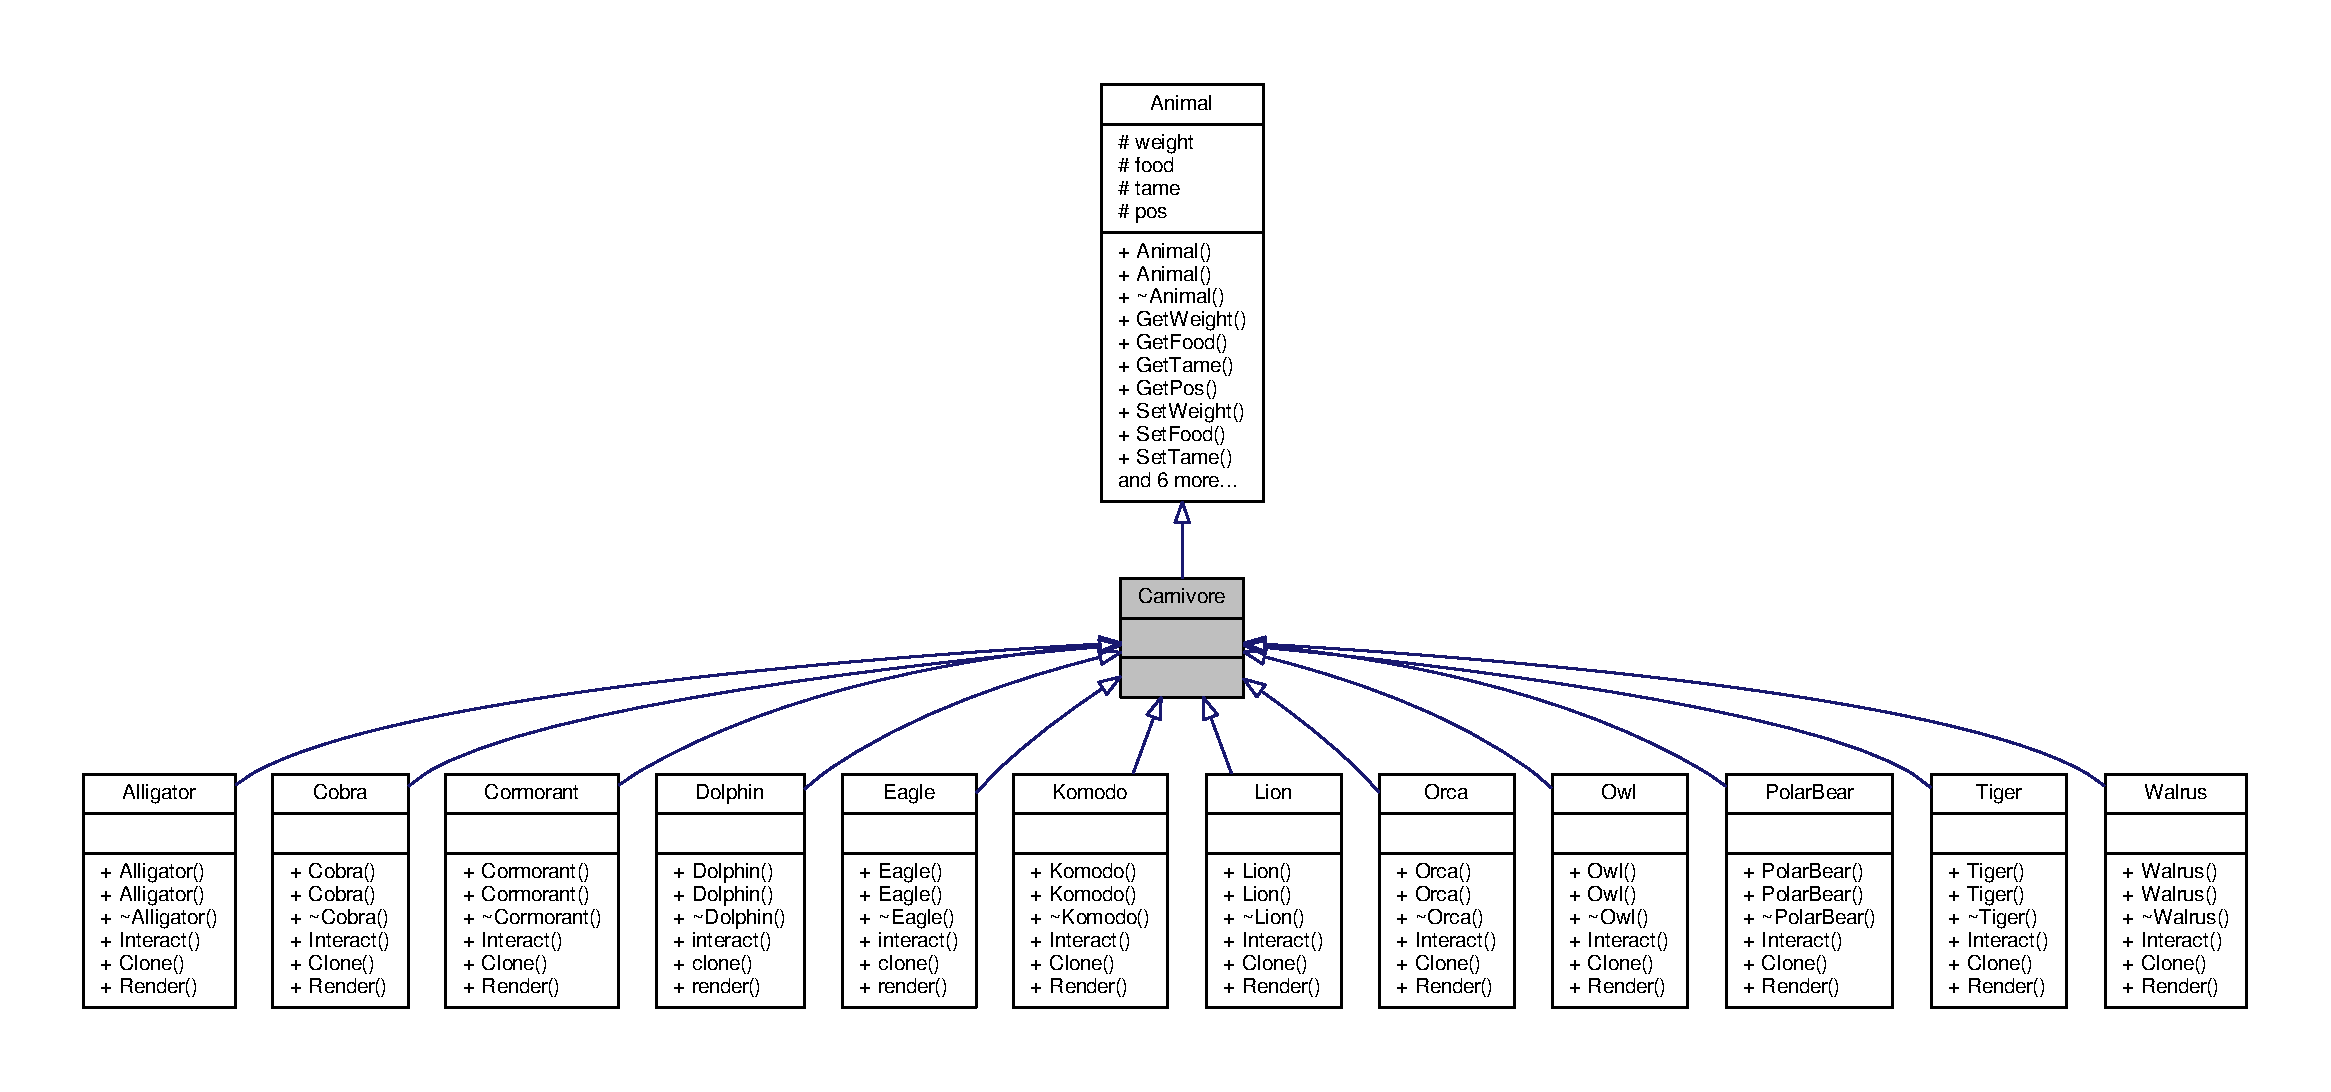
\includegraphics[width=350pt]{classCarnivore__inherit__graph}
\end{center}
\end{figure}


Collaboration diagram for Carnivore\+:
\nopagebreak
\begin{figure}[H]
\begin{center}
\leavevmode
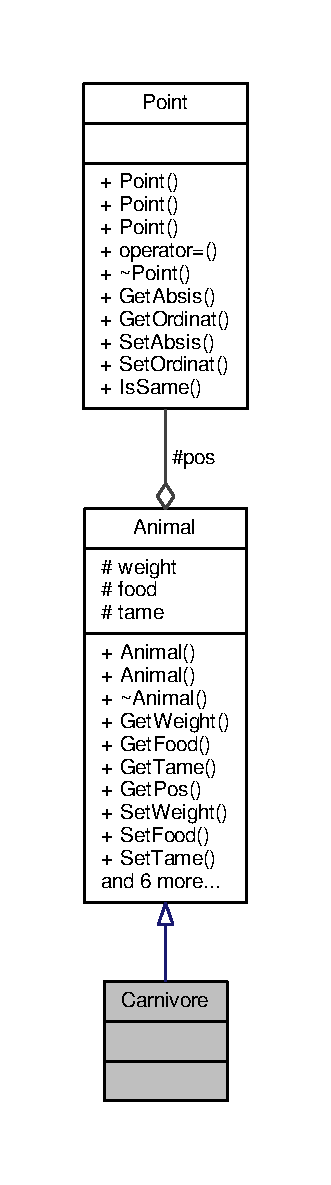
\includegraphics[height=550pt]{classCarnivore__coll__graph}
\end{center}
\end{figure}
\subsection*{Additional Inherited Members}


\subsection{Detailed Description}
Kelas abstrak \hyperlink{classCarnivore}{Carnivore} merupakan kelas bagi animal pemakan daging 

The documentation for this class was generated from the following file\+:\begin{DoxyCompactItemize}
\item 
\hyperlink{carnivore_8h}{carnivore.\+h}\end{DoxyCompactItemize}

\hypertarget{classCell}{}\section{Cell Class Reference}
\label{classCell}\index{Cell@{Cell}}


{\ttfamily \#include $<$cell.\+h$>$}



Collaboration diagram for Cell\+:
\nopagebreak
\begin{figure}[H]
\begin{center}
\leavevmode
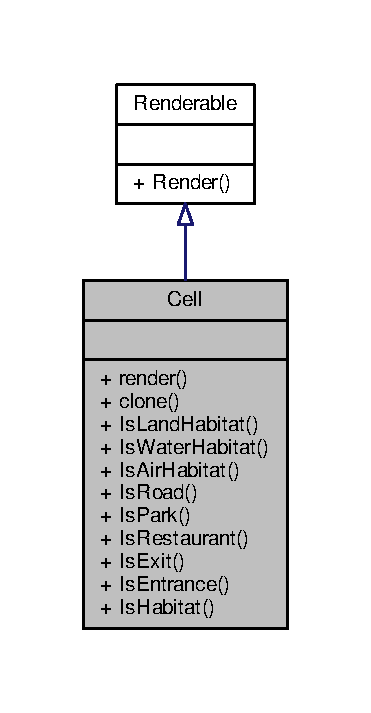
\includegraphics[width=178pt]{classCell__coll__graph}
\end{center}
\end{figure}
\subsection*{Classes}
\begin{DoxyCompactItemize}
\item 
class \hyperlink{classCell_1_1Kelas}{Kelas}
\end{DoxyCompactItemize}
\subsection*{Public Member Functions}
\begin{DoxyCompactItemize}
\item 
\hyperlink{classCell_a394510643e8664cf12b5efaf5cb99f71}{Cell} ()
\begin{DoxyCompactList}\small\item\em Constructor. Menciptakan \hyperlink{classCell}{Cell} kosong. \end{DoxyCompactList}\item 
\hyperlink{classCell_a26ca23bd35b1be145b8c161ac36b9bda}{Cell} (string ot)
\begin{DoxyCompactList}\small\item\em Constructor dengan parameter. Menciptakan \hyperlink{classCell}{Cell} kosong dengan tipe objek ot dan render r. \end{DoxyCompactList}\item 
\hyperlink{classCell_a9fa559f7a28e2b4336c6879ca09304d8}{$\sim$\+Cell} ()
\begin{DoxyCompactList}\small\item\em Destructor. \end{DoxyCompactList}\item 
string \hyperlink{classCell_a6218f05e1d9dcdf9ed61c5196040b1bd}{Get\+Object\+Type} () const 
\begin{DoxyCompactList}\small\item\em Getter untuk object type. \end{DoxyCompactList}\item 
char \hyperlink{classCell_a81e6357d206db3a6e6299029dc2273e5}{Get\+Render} () const 
\begin{DoxyCompactList}\small\item\em Getter untuk render. \end{DoxyCompactList}\item 
void \hyperlink{classCell_ad814dd782c42728917888c893b99b9df}{Set\+Object\+Type} (string ot)
\begin{DoxyCompactList}\small\item\em Setter untuk object type dari \hyperlink{classCell}{Cell}. \end{DoxyCompactList}\item 
bool \hyperlink{classCell_ab44ecb9c8347d20216b335af4e7c3700}{Is\+Habitat} ()
\begin{DoxyCompactList}\small\item\em Is\+Habitat. \end{DoxyCompactList}\item 
bool \hyperlink{classCell_a87c65d914c0be7928836fe8c46b5408e}{Is\+Land\+Habitat} ()
\begin{DoxyCompactList}\small\item\em Is\+Land\+Habitat. \end{DoxyCompactList}\item 
bool \hyperlink{classCell_af270b6bea6287714d585bae539edebc8}{Is\+Air\+Habitat} ()
\begin{DoxyCompactList}\small\item\em Is\+Air\+Habitat. \end{DoxyCompactList}\item 
bool \hyperlink{classCell_a06f065280a20d0008af9980ac4e053d0}{Is\+Water\+Habitat} ()
\begin{DoxyCompactList}\small\item\em Is\+Water\+Habitat. \end{DoxyCompactList}\item 
bool \hyperlink{classCell_a01c619a613088130f13c7d090121cbf5}{Is\+Exit} ()
\begin{DoxyCompactList}\small\item\em Is\+Exit. \end{DoxyCompactList}\item 
bool \hyperlink{classCell_aaaabb185d3c3d8ae23ac70dbc1148768}{Is\+Road} ()
\begin{DoxyCompactList}\small\item\em Is\+Road. \end{DoxyCompactList}\item 
bool \hyperlink{classCell_a15995ac65537db9e5bd3e6e1df7476e3}{Is\+Entrance} ()
\begin{DoxyCompactList}\small\item\em Is\+Entrance. \end{DoxyCompactList}\end{DoxyCompactItemize}
\subsection*{Private Attributes}
\begin{DoxyCompactItemize}
\item 
string \hyperlink{classCell_a800313ab2d6d6686a999e0179695737f}{object\+\_\+type}
\item 
char \hyperlink{classCell_a886f694017e919827f9208d17d3836d3}{render}
\end{DoxyCompactItemize}


\subsection{Constructor \& Destructor Documentation}
\index{Cell@{Cell}!Cell@{Cell}}
\index{Cell@{Cell}!Cell@{Cell}}
\subsubsection[{\texorpdfstring{Cell()}{Cell()}}]{\setlength{\rightskip}{0pt plus 5cm}Cell\+::\+Cell (
\begin{DoxyParamCaption}
{}
\end{DoxyParamCaption}
)}\hypertarget{classCell_a394510643e8664cf12b5efaf5cb99f71}{}\label{classCell_a394510643e8664cf12b5efaf5cb99f71}


Constructor. Menciptakan \hyperlink{classCell}{Cell} kosong. 

\index{Cell@{Cell}!Cell@{Cell}}
\index{Cell@{Cell}!Cell@{Cell}}
\subsubsection[{\texorpdfstring{Cell(string ot)}{Cell(string ot)}}]{\setlength{\rightskip}{0pt plus 5cm}Cell\+::\+Cell (
\begin{DoxyParamCaption}
\item[{string}]{ot}
\end{DoxyParamCaption}
)}\hypertarget{classCell_a26ca23bd35b1be145b8c161ac36b9bda}{}\label{classCell_a26ca23bd35b1be145b8c161ac36b9bda}


Constructor dengan parameter. Menciptakan \hyperlink{classCell}{Cell} kosong dengan tipe objek ot dan render r. 


\begin{DoxyParams}{Parameters}
{\em ot} & Object type dari \hyperlink{classCell}{Cell}. \\
\hline
{\em r} & Render dari \hyperlink{classCell}{Cell}. \\
\hline
\end{DoxyParams}
\index{Cell@{Cell}!````~Cell@{$\sim$\+Cell}}
\index{````~Cell@{$\sim$\+Cell}!Cell@{Cell}}
\subsubsection[{\texorpdfstring{$\sim$\+Cell()}{~Cell()}}]{\setlength{\rightskip}{0pt plus 5cm}Cell\+::$\sim$\+Cell (
\begin{DoxyParamCaption}
{}
\end{DoxyParamCaption}
)}\hypertarget{classCell_a9fa559f7a28e2b4336c6879ca09304d8}{}\label{classCell_a9fa559f7a28e2b4336c6879ca09304d8}


Destructor. 



\subsection{Member Function Documentation}
\index{Cell@{Cell}!Get\+Object\+Type@{Get\+Object\+Type}}
\index{Get\+Object\+Type@{Get\+Object\+Type}!Cell@{Cell}}
\subsubsection[{\texorpdfstring{Get\+Object\+Type() const }{GetObjectType() const }}]{\setlength{\rightskip}{0pt plus 5cm}string Cell\+::\+Get\+Object\+Type (
\begin{DoxyParamCaption}
{}
\end{DoxyParamCaption}
) const}\hypertarget{classCell_a6218f05e1d9dcdf9ed61c5196040b1bd}{}\label{classCell_a6218f05e1d9dcdf9ed61c5196040b1bd}


Getter untuk object type. 

\begin{DoxyReturn}{Returns}
Mengembalikan object type dari \hyperlink{classCell}{Cell}. 
\end{DoxyReturn}
\index{Cell@{Cell}!Get\+Render@{Get\+Render}}
\index{Get\+Render@{Get\+Render}!Cell@{Cell}}
\subsubsection[{\texorpdfstring{Get\+Render() const }{GetRender() const }}]{\setlength{\rightskip}{0pt plus 5cm}char Cell\+::\+Get\+Render (
\begin{DoxyParamCaption}
{}
\end{DoxyParamCaption}
) const}\hypertarget{classCell_a81e6357d206db3a6e6299029dc2273e5}{}\label{classCell_a81e6357d206db3a6e6299029dc2273e5}


Getter untuk render. 

\begin{DoxyReturn}{Returns}
Mengembalikan render dari \hyperlink{classCell}{Cell}. 
\end{DoxyReturn}
\index{Cell@{Cell}!Is\+Air\+Habitat@{Is\+Air\+Habitat}}
\index{Is\+Air\+Habitat@{Is\+Air\+Habitat}!Cell@{Cell}}
\subsubsection[{\texorpdfstring{Is\+Air\+Habitat()}{IsAirHabitat()}}]{\setlength{\rightskip}{0pt plus 5cm}bool Cell\+::\+Is\+Air\+Habitat (
\begin{DoxyParamCaption}
{}
\end{DoxyParamCaption}
)}\hypertarget{classCell_af270b6bea6287714d585bae539edebc8}{}\label{classCell_af270b6bea6287714d585bae539edebc8}


Is\+Air\+Habitat. 

\begin{DoxyReturn}{Returns}
Menghasilkan true jika code pada layar merupakan kode Air Habitat. 
\end{DoxyReturn}
\index{Cell@{Cell}!Is\+Entrance@{Is\+Entrance}}
\index{Is\+Entrance@{Is\+Entrance}!Cell@{Cell}}
\subsubsection[{\texorpdfstring{Is\+Entrance()}{IsEntrance()}}]{\setlength{\rightskip}{0pt plus 5cm}bool Cell\+::\+Is\+Entrance (
\begin{DoxyParamCaption}
{}
\end{DoxyParamCaption}
)}\hypertarget{classCell_a15995ac65537db9e5bd3e6e1df7476e3}{}\label{classCell_a15995ac65537db9e5bd3e6e1df7476e3}


Is\+Entrance. 

\begin{DoxyReturn}{Returns}
Menghasilkan true jika code pada layar merupakan kode Entrance. 
\end{DoxyReturn}
\index{Cell@{Cell}!Is\+Exit@{Is\+Exit}}
\index{Is\+Exit@{Is\+Exit}!Cell@{Cell}}
\subsubsection[{\texorpdfstring{Is\+Exit()}{IsExit()}}]{\setlength{\rightskip}{0pt plus 5cm}bool Cell\+::\+Is\+Exit (
\begin{DoxyParamCaption}
{}
\end{DoxyParamCaption}
)}\hypertarget{classCell_a01c619a613088130f13c7d090121cbf5}{}\label{classCell_a01c619a613088130f13c7d090121cbf5}


Is\+Exit. 

\begin{DoxyReturn}{Returns}
Menghasilkan true jika code pada layar merupakan kode Exit. 
\end{DoxyReturn}
\index{Cell@{Cell}!Is\+Habitat@{Is\+Habitat}}
\index{Is\+Habitat@{Is\+Habitat}!Cell@{Cell}}
\subsubsection[{\texorpdfstring{Is\+Habitat()}{IsHabitat()}}]{\setlength{\rightskip}{0pt plus 5cm}bool Cell\+::\+Is\+Habitat (
\begin{DoxyParamCaption}
{}
\end{DoxyParamCaption}
)}\hypertarget{classCell_ab44ecb9c8347d20216b335af4e7c3700}{}\label{classCell_ab44ecb9c8347d20216b335af4e7c3700}


Is\+Habitat. 

\begin{DoxyReturn}{Returns}
Menghasilkan true jika code pada layar merupakan kode Land, Air, atau Water Habitat. 
\end{DoxyReturn}
\index{Cell@{Cell}!Is\+Land\+Habitat@{Is\+Land\+Habitat}}
\index{Is\+Land\+Habitat@{Is\+Land\+Habitat}!Cell@{Cell}}
\subsubsection[{\texorpdfstring{Is\+Land\+Habitat()}{IsLandHabitat()}}]{\setlength{\rightskip}{0pt plus 5cm}bool Cell\+::\+Is\+Land\+Habitat (
\begin{DoxyParamCaption}
{}
\end{DoxyParamCaption}
)}\hypertarget{classCell_a87c65d914c0be7928836fe8c46b5408e}{}\label{classCell_a87c65d914c0be7928836fe8c46b5408e}


Is\+Land\+Habitat. 

\begin{DoxyReturn}{Returns}
Menghasilkan true jika code pada layar merupakan kode Land Habitat. 
\end{DoxyReturn}
\index{Cell@{Cell}!Is\+Road@{Is\+Road}}
\index{Is\+Road@{Is\+Road}!Cell@{Cell}}
\subsubsection[{\texorpdfstring{Is\+Road()}{IsRoad()}}]{\setlength{\rightskip}{0pt plus 5cm}bool Cell\+::\+Is\+Road (
\begin{DoxyParamCaption}
{}
\end{DoxyParamCaption}
)}\hypertarget{classCell_aaaabb185d3c3d8ae23ac70dbc1148768}{}\label{classCell_aaaabb185d3c3d8ae23ac70dbc1148768}


Is\+Road. 

\begin{DoxyReturn}{Returns}
Menghasilkan true jika code pada layar merupakan kode Road. 
\end{DoxyReturn}
\index{Cell@{Cell}!Is\+Water\+Habitat@{Is\+Water\+Habitat}}
\index{Is\+Water\+Habitat@{Is\+Water\+Habitat}!Cell@{Cell}}
\subsubsection[{\texorpdfstring{Is\+Water\+Habitat()}{IsWaterHabitat()}}]{\setlength{\rightskip}{0pt plus 5cm}bool Cell\+::\+Is\+Water\+Habitat (
\begin{DoxyParamCaption}
{}
\end{DoxyParamCaption}
)}\hypertarget{classCell_a06f065280a20d0008af9980ac4e053d0}{}\label{classCell_a06f065280a20d0008af9980ac4e053d0}


Is\+Water\+Habitat. 

\begin{DoxyReturn}{Returns}
Menghasilkan true jika code pada layar merupakan kode Water Habitat. 
\end{DoxyReturn}
\index{Cell@{Cell}!Set\+Object\+Type@{Set\+Object\+Type}}
\index{Set\+Object\+Type@{Set\+Object\+Type}!Cell@{Cell}}
\subsubsection[{\texorpdfstring{Set\+Object\+Type(string ot)}{SetObjectType(string ot)}}]{\setlength{\rightskip}{0pt plus 5cm}void Cell\+::\+Set\+Object\+Type (
\begin{DoxyParamCaption}
\item[{string}]{ot}
\end{DoxyParamCaption}
)}\hypertarget{classCell_ad814dd782c42728917888c893b99b9df}{}\label{classCell_ad814dd782c42728917888c893b99b9df}


Setter untuk object type dari \hyperlink{classCell}{Cell}. 


\begin{DoxyParams}{Parameters}
{\em ot} & Nilai object type yang akan di-\/set pada \hyperlink{classCell}{Cell}. \\
\hline
\end{DoxyParams}


\subsection{Member Data Documentation}
\index{Cell@{Cell}!object\+\_\+type@{object\+\_\+type}}
\index{object\+\_\+type@{object\+\_\+type}!Cell@{Cell}}
\subsubsection[{\texorpdfstring{object\+\_\+type}{object_type}}]{\setlength{\rightskip}{0pt plus 5cm}string Cell\+::object\+\_\+type\hspace{0.3cm}{\ttfamily [private]}}\hypertarget{classCell_a800313ab2d6d6686a999e0179695737f}{}\label{classCell_a800313ab2d6d6686a999e0179695737f}
\index{Cell@{Cell}!render@{render}}
\index{render@{render}!Cell@{Cell}}
\subsubsection[{\texorpdfstring{render}{render}}]{\setlength{\rightskip}{0pt plus 5cm}char Cell\+::render\hspace{0.3cm}{\ttfamily [private]}}\hypertarget{classCell_a886f694017e919827f9208d17d3836d3}{}\label{classCell_a886f694017e919827f9208d17d3836d3}


The documentation for this class was generated from the following files\+:\begin{DoxyCompactItemize}
\item 
cell/\hyperlink{cell_8h}{cell.\+h}\item 
cell/\hyperlink{cell_8cpp}{cell.\+cpp}\end{DoxyCompactItemize}

\hypertarget{classCobra}{}\section{Cobra Class Reference}
\label{classCobra}\index{Cobra@{Cobra}}


{\ttfamily \#include $<$cobra.\+h$>$}



Inheritance diagram for Cobra\+:
% FIG 0


Collaboration diagram for Cobra\+:
% FIG 1
\subsection*{Public Member Functions}
\begin{DoxyCompactItemize}
\item 
\hyperlink{classCobra_acc0ec4a84ca7a0ea5e53aa1e8cabd268}{Cobra} ()
\begin{DoxyCompactList}\small\item\em Constructor. Menciptakan objek \hyperlink{classCobra}{Cobra}. \end{DoxyCompactList}\item 
\hyperlink{classCobra_ad1df7df30cea151706031ee0b9f28abd}{Cobra} (float w, float f, bool t)
\begin{DoxyCompactList}\small\item\em Constructor dengan parameter. Menciptakan objek \hyperlink{classCobra}{Cobra} dengan berat w, jumlah makanan f, dan status jinak t. \end{DoxyCompactList}\item 
virtual \hyperlink{classCobra_ac109599e6a8c9a01e852c54fb6fa2687}{$\sim$\+Cobra} ()
\begin{DoxyCompactList}\small\item\em Destructor. \end{DoxyCompactList}\item 
string \hyperlink{classCobra_aa8dd0878e3d654e51bec9592c88bcab5}{Interact} ()
\begin{DoxyCompactList}\small\item\em Interaksi yang dilakukan \hyperlink{classCobra}{Cobra}. \end{DoxyCompactList}\item 
virtual \hyperlink{classCobra}{Cobra} $\ast$ \hyperlink{classCobra_a1bfd2035a0a700b6362b1853cb12949b}{Clone} () const 
\begin{DoxyCompactList}\small\item\em Melakukan cloning untuk menciptakan objek \hyperlink{classCobra}{Cobra} baru. \end{DoxyCompactList}\item 
char \hyperlink{classCobra_abca7da2ee55ce825dc49f4f9a3e87208}{Render} ()
\begin{DoxyCompactList}\small\item\em Render dari \hyperlink{classCobra}{Cobra}. \end{DoxyCompactList}\end{DoxyCompactItemize}
\subsection*{Additional Inherited Members}


\subsection{Detailed Description}
Kelas \hyperlink{classCobra}{Cobra} merupakan kelas untuk real object \hyperlink{classCobra}{Cobra} 

\subsection{Constructor \& Destructor Documentation}
\index{Cobra@{Cobra}!Cobra@{Cobra}}
\index{Cobra@{Cobra}!Cobra@{Cobra}}
\subsubsection[{\texorpdfstring{Cobra()}{Cobra()}}]{\setlength{\rightskip}{0pt plus 5cm}Cobra\+::\+Cobra (
\begin{DoxyParamCaption}
{}
\end{DoxyParamCaption}
)\hspace{0.3cm}{\ttfamily [inline]}}\hypertarget{classCobra_acc0ec4a84ca7a0ea5e53aa1e8cabd268}{}\label{classCobra_acc0ec4a84ca7a0ea5e53aa1e8cabd268}


Constructor. Menciptakan objek \hyperlink{classCobra}{Cobra}. 

\index{Cobra@{Cobra}!Cobra@{Cobra}}
\index{Cobra@{Cobra}!Cobra@{Cobra}}
\subsubsection[{\texorpdfstring{Cobra(float w, float f, bool t)}{Cobra(float w, float f, bool t)}}]{\setlength{\rightskip}{0pt plus 5cm}Cobra\+::\+Cobra (
\begin{DoxyParamCaption}
\item[{float}]{w, }
\item[{float}]{f, }
\item[{bool}]{t}
\end{DoxyParamCaption}
)\hspace{0.3cm}{\ttfamily [inline]}}\hypertarget{classCobra_ad1df7df30cea151706031ee0b9f28abd}{}\label{classCobra_ad1df7df30cea151706031ee0b9f28abd}


Constructor dengan parameter. Menciptakan objek \hyperlink{classCobra}{Cobra} dengan berat w, jumlah makanan f, dan status jinak t. 


\begin{DoxyParams}{Parameters}
{\em w} & Berat \hyperlink{classCobra}{Cobra}. \\
\hline
{\em f} & Jumlah makanan \hyperlink{classCobra}{Cobra}. \\
\hline
{\em t} & Status jinak \hyperlink{classCobra}{Cobra}. \\
\hline
\end{DoxyParams}
\index{Cobra@{Cobra}!````~Cobra@{$\sim$\+Cobra}}
\index{````~Cobra@{$\sim$\+Cobra}!Cobra@{Cobra}}
\subsubsection[{\texorpdfstring{$\sim$\+Cobra()}{~Cobra()}}]{\setlength{\rightskip}{0pt plus 5cm}virtual Cobra\+::$\sim$\+Cobra (
\begin{DoxyParamCaption}
{}
\end{DoxyParamCaption}
)\hspace{0.3cm}{\ttfamily [inline]}, {\ttfamily [virtual]}}\hypertarget{classCobra_ac109599e6a8c9a01e852c54fb6fa2687}{}\label{classCobra_ac109599e6a8c9a01e852c54fb6fa2687}


Destructor. 



\subsection{Member Function Documentation}
\index{Cobra@{Cobra}!Clone@{Clone}}
\index{Clone@{Clone}!Cobra@{Cobra}}
\subsubsection[{\texorpdfstring{Clone() const }{Clone() const }}]{\setlength{\rightskip}{0pt plus 5cm}virtual {\bf Cobra}$\ast$ Cobra\+::\+Clone (
\begin{DoxyParamCaption}
{}
\end{DoxyParamCaption}
) const\hspace{0.3cm}{\ttfamily [inline]}, {\ttfamily [virtual]}}\hypertarget{classCobra_a1bfd2035a0a700b6362b1853cb12949b}{}\label{classCobra_a1bfd2035a0a700b6362b1853cb12949b}


Melakukan cloning untuk menciptakan objek \hyperlink{classCobra}{Cobra} baru. 

\begin{DoxyReturn}{Returns}
Mengembalikan pointer to \hyperlink{classCobra}{Cobra} objek tersebut. 
\end{DoxyReturn}


Implements \hyperlink{classAnimal_a3fc95e2a588b653b9b315e6c7a29c89f}{Animal}.

\index{Cobra@{Cobra}!Interact@{Interact}}
\index{Interact@{Interact}!Cobra@{Cobra}}
\subsubsection[{\texorpdfstring{Interact()}{Interact()}}]{\setlength{\rightskip}{0pt plus 5cm}string Cobra\+::\+Interact (
\begin{DoxyParamCaption}
{}
\end{DoxyParamCaption}
)\hspace{0.3cm}{\ttfamily [inline]}, {\ttfamily [virtual]}}\hypertarget{classCobra_aa8dd0878e3d654e51bec9592c88bcab5}{}\label{classCobra_aa8dd0878e3d654e51bec9592c88bcab5}


Interaksi yang dilakukan \hyperlink{classCobra}{Cobra}. 

\begin{DoxyReturn}{Returns}
Mengembalikan string yang merepresentasikan suara \hyperlink{classCobra}{Cobra}. 
\end{DoxyReturn}


Implements \hyperlink{classAnimal_ad5a55fb0355a9425fee6611003d9892c}{Animal}.

\index{Cobra@{Cobra}!Render@{Render}}
\index{Render@{Render}!Cobra@{Cobra}}
\subsubsection[{\texorpdfstring{Render()}{Render()}}]{\setlength{\rightskip}{0pt plus 5cm}char Cobra\+::\+Render (
\begin{DoxyParamCaption}
{}
\end{DoxyParamCaption}
)\hspace{0.3cm}{\ttfamily [inline]}, {\ttfamily [virtual]}}\hypertarget{classCobra_abca7da2ee55ce825dc49f4f9a3e87208}{}\label{classCobra_abca7da2ee55ce825dc49f4f9a3e87208}


Render dari \hyperlink{classCobra}{Cobra}. 

\begin{DoxyReturn}{Returns}
Mengembalikan char yang merupakan representasi kode \hyperlink{classCobra}{Cobra}. 
\end{DoxyReturn}


Implements \hyperlink{classAnimal_a43a47c0f41d211128e04abc6add53def}{Animal}.



The documentation for this class was generated from the following file\+:\begin{DoxyCompactItemize}
\item 
cobra/\hyperlink{cobra_8h}{cobra.\+h}\end{DoxyCompactItemize}

\hypertarget{classCormorant}{}\section{Cormorant Class Reference}
\label{classCormorant}\index{Cormorant@{Cormorant}}


{\ttfamily \#include $<$cormorant.\+h$>$}



Inheritance diagram for Cormorant\+:
\nopagebreak
\begin{figure}[H]
\begin{center}
\leavevmode
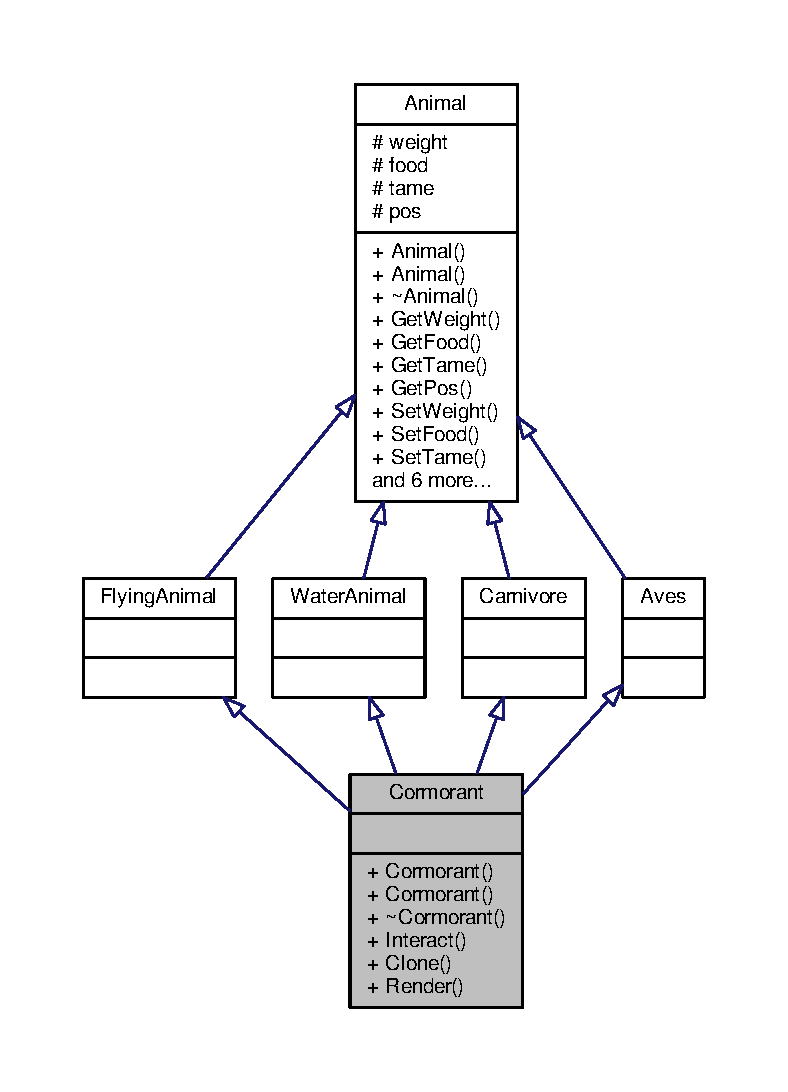
\includegraphics[width=210pt]{classCormorant__inherit__graph}
\end{center}
\end{figure}


Collaboration diagram for Cormorant\+:
\nopagebreak
\begin{figure}[H]
\begin{center}
\leavevmode
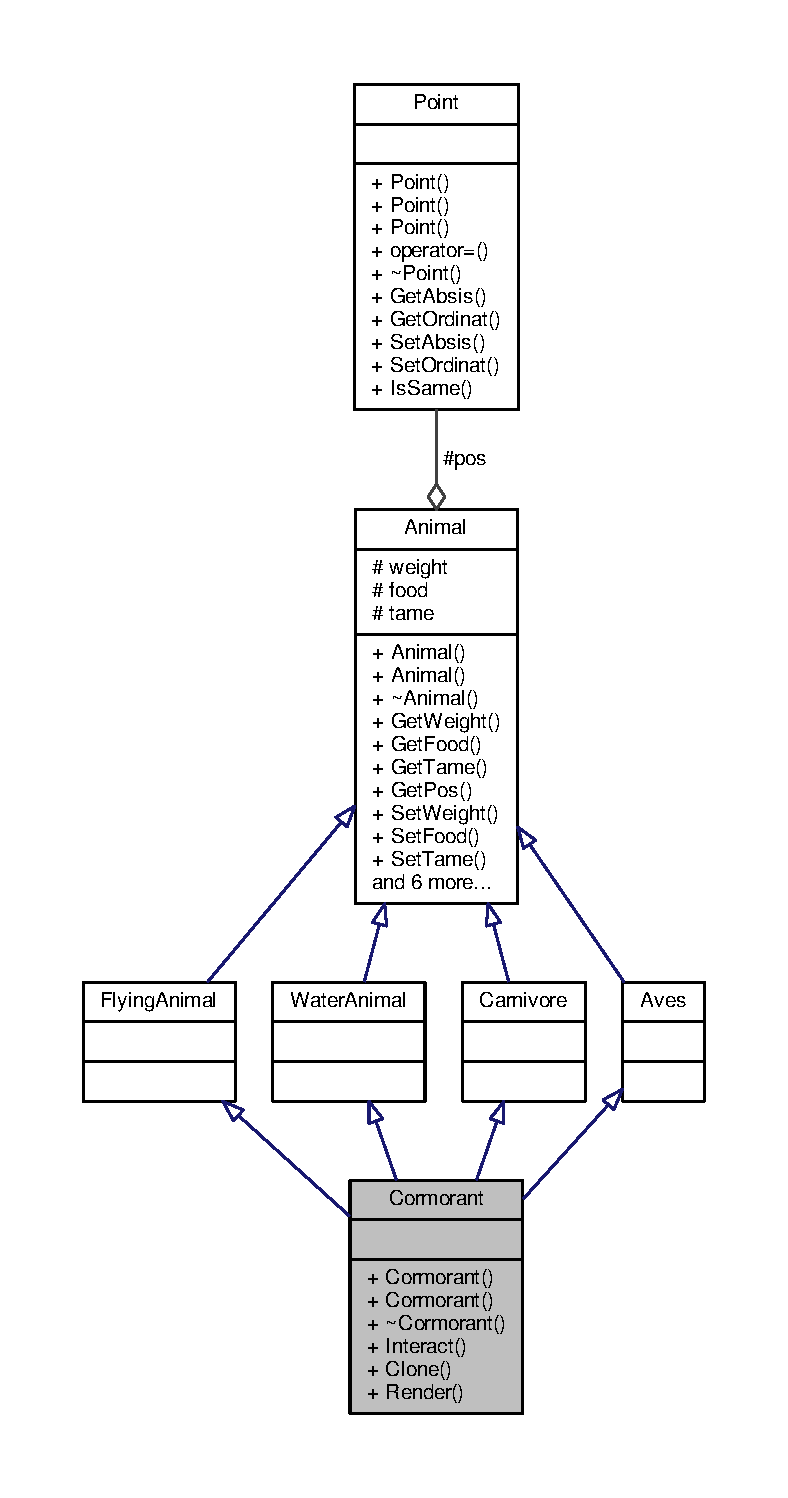
\includegraphics[height=550pt]{classCormorant__coll__graph}
\end{center}
\end{figure}
\subsection*{Public Member Functions}
\begin{DoxyCompactItemize}
\item 
\hyperlink{classCormorant_a1c93b60af03db473c444783df366a2ae}{Cormorant} ()
\begin{DoxyCompactList}\small\item\em Constructor. Menciptakan objek \hyperlink{classCormorant}{Cormorant}. \end{DoxyCompactList}\item 
virtual \hyperlink{classCormorant_af24217c3b840dcf95b0961d68a241034}{$\sim$\+Cormorant} ()
\begin{DoxyCompactList}\small\item\em Destructor. \end{DoxyCompactList}\item 
string \hyperlink{classCormorant_af28984652ae999452d20aed885f0185a}{Interact} ()
\begin{DoxyCompactList}\small\item\em Interaksi yang dilakukan \hyperlink{classCormorant}{Cormorant}. \end{DoxyCompactList}\item 
virtual \hyperlink{classCormorant}{Cormorant} $\ast$ \hyperlink{classCormorant_a7be371562fab8ab5c2e9e72386ee9aa2}{Clone} () const 
\begin{DoxyCompactList}\small\item\em Melakukan cloning untuk menciptakan objek \hyperlink{classCormorant}{Cormorant} baru. \end{DoxyCompactList}\item 
char \hyperlink{classCormorant_a6d388885acfc98de6020a01b90259dac}{Render} ()
\begin{DoxyCompactList}\small\item\em Render dari \hyperlink{classCormorant}{Cormorant}. \end{DoxyCompactList}\end{DoxyCompactItemize}
\subsection*{Additional Inherited Members}


\subsection{Detailed Description}
Kelas \hyperlink{classCormorant}{Cormorant} merupakan kelas untuk real object \hyperlink{classCormorant}{Cormorant} 

\subsection{Constructor \& Destructor Documentation}
\index{Cormorant@{Cormorant}!Cormorant@{Cormorant}}
\index{Cormorant@{Cormorant}!Cormorant@{Cormorant}}
\subsubsection[{\texorpdfstring{Cormorant()}{Cormorant()}}]{\setlength{\rightskip}{0pt plus 5cm}Cormorant\+::\+Cormorant (
\begin{DoxyParamCaption}
{}
\end{DoxyParamCaption}
)\hspace{0.3cm}{\ttfamily [inline]}}\hypertarget{classCormorant_a1c93b60af03db473c444783df366a2ae}{}\label{classCormorant_a1c93b60af03db473c444783df366a2ae}


Constructor. Menciptakan objek \hyperlink{classCormorant}{Cormorant}. 

\index{Cormorant@{Cormorant}!````~Cormorant@{$\sim$\+Cormorant}}
\index{````~Cormorant@{$\sim$\+Cormorant}!Cormorant@{Cormorant}}
\subsubsection[{\texorpdfstring{$\sim$\+Cormorant()}{~Cormorant()}}]{\setlength{\rightskip}{0pt plus 5cm}virtual Cormorant\+::$\sim$\+Cormorant (
\begin{DoxyParamCaption}
{}
\end{DoxyParamCaption}
)\hspace{0.3cm}{\ttfamily [inline]}, {\ttfamily [virtual]}}\hypertarget{classCormorant_af24217c3b840dcf95b0961d68a241034}{}\label{classCormorant_af24217c3b840dcf95b0961d68a241034}


Destructor. 



\subsection{Member Function Documentation}
\index{Cormorant@{Cormorant}!Clone@{Clone}}
\index{Clone@{Clone}!Cormorant@{Cormorant}}
\subsubsection[{\texorpdfstring{Clone() const }{Clone() const }}]{\setlength{\rightskip}{0pt plus 5cm}virtual {\bf Cormorant}$\ast$ Cormorant\+::\+Clone (
\begin{DoxyParamCaption}
{}
\end{DoxyParamCaption}
) const\hspace{0.3cm}{\ttfamily [inline]}, {\ttfamily [virtual]}}\hypertarget{classCormorant_a7be371562fab8ab5c2e9e72386ee9aa2}{}\label{classCormorant_a7be371562fab8ab5c2e9e72386ee9aa2}


Melakukan cloning untuk menciptakan objek \hyperlink{classCormorant}{Cormorant} baru. 

\begin{DoxyReturn}{Returns}
Mengembalikan pointer to \hyperlink{classCormorant}{Cormorant} objek tersebut. 
\end{DoxyReturn}


Implements \hyperlink{classAnimal_a3fc95e2a588b653b9b315e6c7a29c89f}{Animal}.

\index{Cormorant@{Cormorant}!Interact@{Interact}}
\index{Interact@{Interact}!Cormorant@{Cormorant}}
\subsubsection[{\texorpdfstring{Interact()}{Interact()}}]{\setlength{\rightskip}{0pt plus 5cm}string Cormorant\+::\+Interact (
\begin{DoxyParamCaption}
{}
\end{DoxyParamCaption}
)\hspace{0.3cm}{\ttfamily [inline]}, {\ttfamily [virtual]}}\hypertarget{classCormorant_af28984652ae999452d20aed885f0185a}{}\label{classCormorant_af28984652ae999452d20aed885f0185a}


Interaksi yang dilakukan \hyperlink{classCormorant}{Cormorant}. 

\begin{DoxyReturn}{Returns}
Mengembalikan string yang merepresentasikan suara \hyperlink{classCormorant}{Cormorant}. 
\end{DoxyReturn}


Implements \hyperlink{classAnimal_ad5a55fb0355a9425fee6611003d9892c}{Animal}.

\index{Cormorant@{Cormorant}!Render@{Render}}
\index{Render@{Render}!Cormorant@{Cormorant}}
\subsubsection[{\texorpdfstring{Render()}{Render()}}]{\setlength{\rightskip}{0pt plus 5cm}char Cormorant\+::\+Render (
\begin{DoxyParamCaption}
{}
\end{DoxyParamCaption}
)\hspace{0.3cm}{\ttfamily [inline]}, {\ttfamily [virtual]}}\hypertarget{classCormorant_a6d388885acfc98de6020a01b90259dac}{}\label{classCormorant_a6d388885acfc98de6020a01b90259dac}


Render dari \hyperlink{classCormorant}{Cormorant}. 

\begin{DoxyReturn}{Returns}
Mengembalikan char yang merupakan representasi kode \hyperlink{classCormorant}{Cormorant}. 
\end{DoxyReturn}


Implements \hyperlink{classAnimal_a43a47c0f41d211128e04abc6add53def}{Animal}.



The documentation for this class was generated from the following file\+:\begin{DoxyCompactItemize}
\item 
cormorant/\hyperlink{cormorant_8h}{cormorant.\+h}\end{DoxyCompactItemize}

\hypertarget{classDolphin}{}\section{Dolphin Class Reference}
\label{classDolphin}\index{Dolphin@{Dolphin}}


{\ttfamily \#include $<$dolphin.\+h$>$}



Inheritance diagram for Dolphin\+:
\nopagebreak
\begin{figure}[H]
\begin{center}
\leavevmode
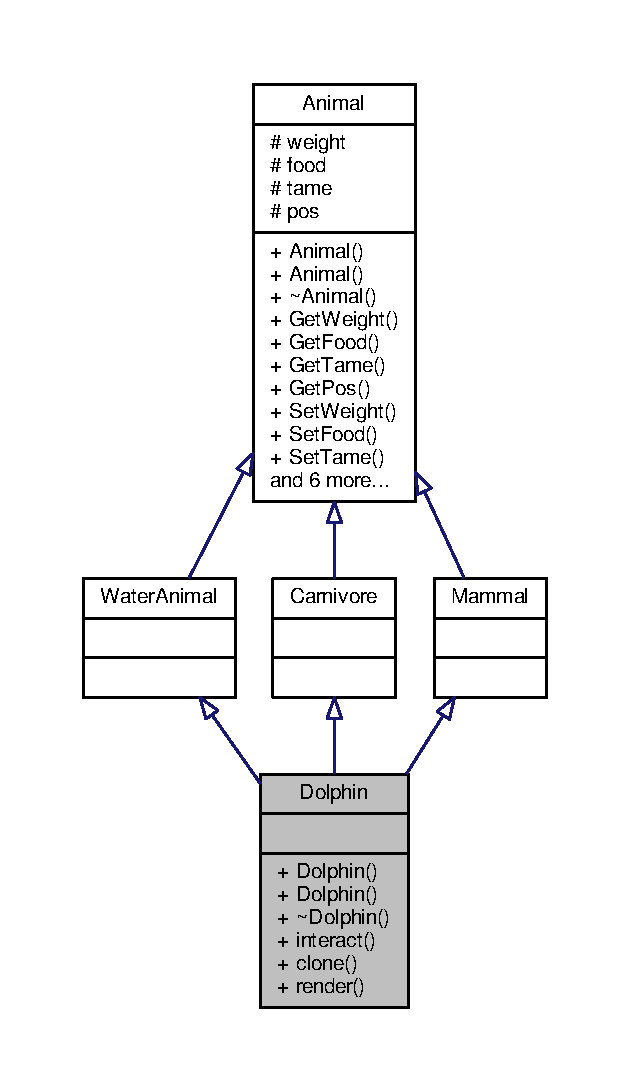
\includegraphics[width=303pt]{classDolphin__inherit__graph}
\end{center}
\end{figure}


Collaboration diagram for Dolphin\+:
\nopagebreak
\begin{figure}[H]
\begin{center}
\leavevmode
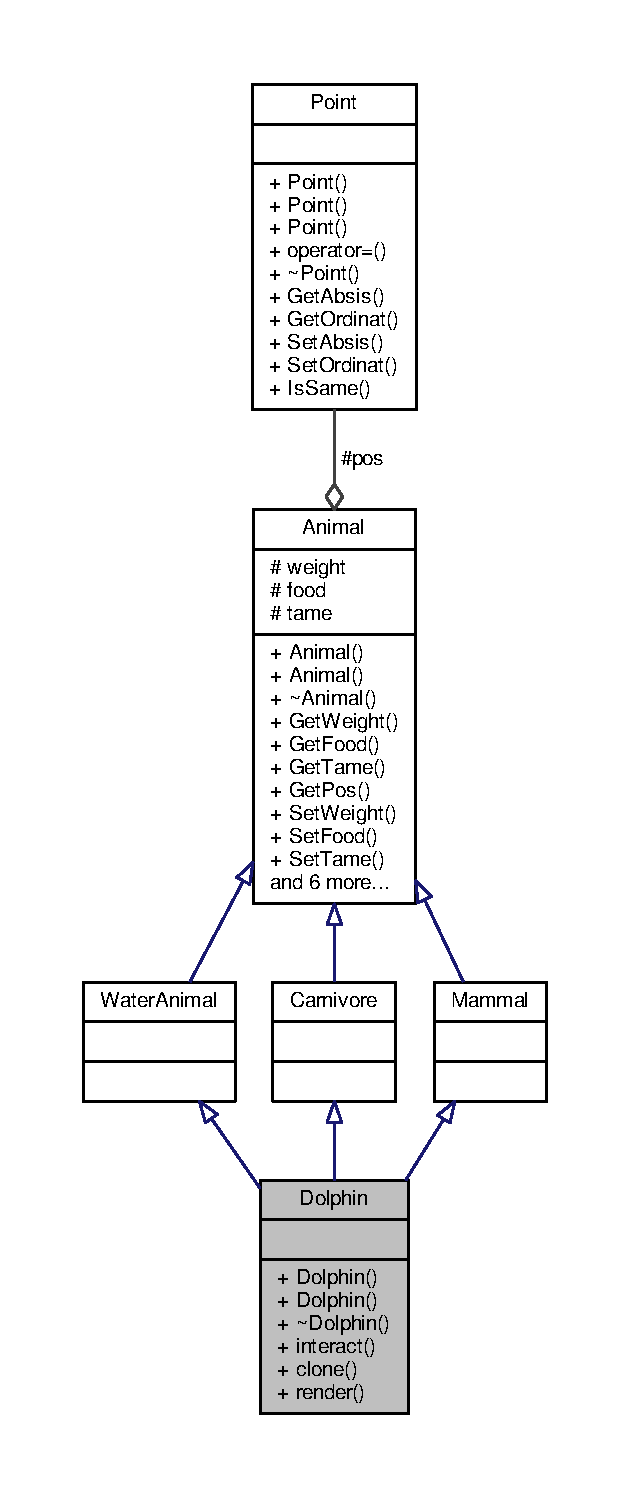
\includegraphics[height=550pt]{classDolphin__coll__graph}
\end{center}
\end{figure}
\subsection*{Public Member Functions}
\begin{DoxyCompactItemize}
\item 
\hyperlink{classDolphin_a571a22b2c3cece5c8175ff49640b35bc}{Dolphin} ()
\begin{DoxyCompactList}\small\item\em Constructor. Menciptakan objek \hyperlink{classDolphin}{Dolphin}. \end{DoxyCompactList}\item 
\hyperlink{classDolphin_a024370cf7beeaef3fbdcdd5fef09e6ef}{Dolphin} (float w, float f, bool t)
\begin{DoxyCompactList}\small\item\em Constructor dengan parameter. Menciptakan objek \hyperlink{classDolphin}{Dolphin} dengan berat w, jumlah makanan f, dan status jinak t. \end{DoxyCompactList}\item 
virtual \hyperlink{classDolphin_a5c11950fe5675f3c36001f20a12343af}{$\sim$\+Dolphin} ()
\begin{DoxyCompactList}\small\item\em Destructor. \end{DoxyCompactList}\item 
string \hyperlink{classDolphin_a592506c38c185d7d383ae755deb9bd72}{Interact} ()
\begin{DoxyCompactList}\small\item\em Interaksi yang dilakukan \hyperlink{classDolphin}{Dolphin}. \end{DoxyCompactList}\item 
virtual \hyperlink{classDolphin}{Dolphin} $\ast$ \hyperlink{classDolphin_a4be3892432206693d2fae815303e07c4}{Clone} () const 
\begin{DoxyCompactList}\small\item\em Melakukan cloning untuk menciptakan objek \hyperlink{classDolphin}{Dolphin} baru. \end{DoxyCompactList}\item 
char \hyperlink{classDolphin_aa051d8ebe93c1c11b503ae76d07cd178}{Render} ()
\begin{DoxyCompactList}\small\item\em Render dari \hyperlink{classDolphin}{Dolphin}. \end{DoxyCompactList}\end{DoxyCompactItemize}
\subsection*{Additional Inherited Members}


\subsection{Detailed Description}
Kelas \hyperlink{classDolphin}{Dolphin} merupakan kelas untuk real object \hyperlink{classDolphin}{Dolphin} 

\subsection{Constructor \& Destructor Documentation}
\index{Dolphin@{Dolphin}!Dolphin@{Dolphin}}
\index{Dolphin@{Dolphin}!Dolphin@{Dolphin}}
\subsubsection[{\texorpdfstring{Dolphin()}{Dolphin()}}]{\setlength{\rightskip}{0pt plus 5cm}Dolphin\+::\+Dolphin (
\begin{DoxyParamCaption}
{}
\end{DoxyParamCaption}
)\hspace{0.3cm}{\ttfamily [inline]}}\hypertarget{classDolphin_a571a22b2c3cece5c8175ff49640b35bc}{}\label{classDolphin_a571a22b2c3cece5c8175ff49640b35bc}


Constructor. Menciptakan objek \hyperlink{classDolphin}{Dolphin}. 

\index{Dolphin@{Dolphin}!Dolphin@{Dolphin}}
\index{Dolphin@{Dolphin}!Dolphin@{Dolphin}}
\subsubsection[{\texorpdfstring{Dolphin(float w, float f, bool t)}{Dolphin(float w, float f, bool t)}}]{\setlength{\rightskip}{0pt plus 5cm}Dolphin\+::\+Dolphin (
\begin{DoxyParamCaption}
\item[{float}]{w, }
\item[{float}]{f, }
\item[{bool}]{t}
\end{DoxyParamCaption}
)\hspace{0.3cm}{\ttfamily [inline]}}\hypertarget{classDolphin_a024370cf7beeaef3fbdcdd5fef09e6ef}{}\label{classDolphin_a024370cf7beeaef3fbdcdd5fef09e6ef}


Constructor dengan parameter. Menciptakan objek \hyperlink{classDolphin}{Dolphin} dengan berat w, jumlah makanan f, dan status jinak t. 


\begin{DoxyParams}{Parameters}
{\em w} & Berat \hyperlink{classDolphin}{Dolphin}. \\
\hline
{\em f} & Jumlah makanan \hyperlink{classDolphin}{Dolphin}. \\
\hline
{\em t} & Status jinak \hyperlink{classDolphin}{Dolphin}. \\
\hline
\end{DoxyParams}
\index{Dolphin@{Dolphin}!````~Dolphin@{$\sim$\+Dolphin}}
\index{````~Dolphin@{$\sim$\+Dolphin}!Dolphin@{Dolphin}}
\subsubsection[{\texorpdfstring{$\sim$\+Dolphin()}{~Dolphin()}}]{\setlength{\rightskip}{0pt plus 5cm}virtual Dolphin\+::$\sim$\+Dolphin (
\begin{DoxyParamCaption}
{}
\end{DoxyParamCaption}
)\hspace{0.3cm}{\ttfamily [inline]}, {\ttfamily [virtual]}}\hypertarget{classDolphin_a5c11950fe5675f3c36001f20a12343af}{}\label{classDolphin_a5c11950fe5675f3c36001f20a12343af}


Destructor. 



\subsection{Member Function Documentation}
\index{Dolphin@{Dolphin}!Clone@{Clone}}
\index{Clone@{Clone}!Dolphin@{Dolphin}}
\subsubsection[{\texorpdfstring{Clone() const }{Clone() const }}]{\setlength{\rightskip}{0pt plus 5cm}virtual {\bf Dolphin}$\ast$ Dolphin\+::\+Clone (
\begin{DoxyParamCaption}
{}
\end{DoxyParamCaption}
) const\hspace{0.3cm}{\ttfamily [inline]}, {\ttfamily [virtual]}}\hypertarget{classDolphin_a4be3892432206693d2fae815303e07c4}{}\label{classDolphin_a4be3892432206693d2fae815303e07c4}


Melakukan cloning untuk menciptakan objek \hyperlink{classDolphin}{Dolphin} baru. 

\begin{DoxyReturn}{Returns}
Mengembalikan pointer to \hyperlink{classDolphin}{Dolphin} objek tersebut. 
\end{DoxyReturn}


Implements \hyperlink{classAnimal_a3fc95e2a588b653b9b315e6c7a29c89f}{Animal}.

\index{Dolphin@{Dolphin}!Interact@{Interact}}
\index{Interact@{Interact}!Dolphin@{Dolphin}}
\subsubsection[{\texorpdfstring{Interact()}{Interact()}}]{\setlength{\rightskip}{0pt plus 5cm}string Dolphin\+::\+Interact (
\begin{DoxyParamCaption}
{}
\end{DoxyParamCaption}
)\hspace{0.3cm}{\ttfamily [inline]}, {\ttfamily [virtual]}}\hypertarget{classDolphin_a592506c38c185d7d383ae755deb9bd72}{}\label{classDolphin_a592506c38c185d7d383ae755deb9bd72}


Interaksi yang dilakukan \hyperlink{classDolphin}{Dolphin}. 

\begin{DoxyReturn}{Returns}
Mengembalikan string yang merepresentasikan suara Dolpin. 
\end{DoxyReturn}


Implements \hyperlink{classAnimal_ad5a55fb0355a9425fee6611003d9892c}{Animal}.

\index{Dolphin@{Dolphin}!Render@{Render}}
\index{Render@{Render}!Dolphin@{Dolphin}}
\subsubsection[{\texorpdfstring{Render()}{Render()}}]{\setlength{\rightskip}{0pt plus 5cm}char Dolphin\+::\+Render (
\begin{DoxyParamCaption}
{}
\end{DoxyParamCaption}
)\hspace{0.3cm}{\ttfamily [inline]}, {\ttfamily [virtual]}}\hypertarget{classDolphin_aa051d8ebe93c1c11b503ae76d07cd178}{}\label{classDolphin_aa051d8ebe93c1c11b503ae76d07cd178}


Render dari \hyperlink{classDolphin}{Dolphin}. 

\begin{DoxyReturn}{Returns}
Mengembalikan char yang merupakan representasi kode \hyperlink{classDolphin}{Dolphin}. 
\end{DoxyReturn}


Implements \hyperlink{classAnimal_a43a47c0f41d211128e04abc6add53def}{Animal}.



The documentation for this class was generated from the following file\+:\begin{DoxyCompactItemize}
\item 
dolphin/\hyperlink{dolphin_8h}{dolphin.\+h}\end{DoxyCompactItemize}

\hypertarget{classDriver}{}\section{Driver Class Reference}
\label{classDriver}\index{Driver@{Driver}}


{\ttfamily \#include $<$driver.\+h$>$}



Collaboration diagram for Driver\+:
\nopagebreak
\begin{figure}[H]
\begin{center}
\leavevmode
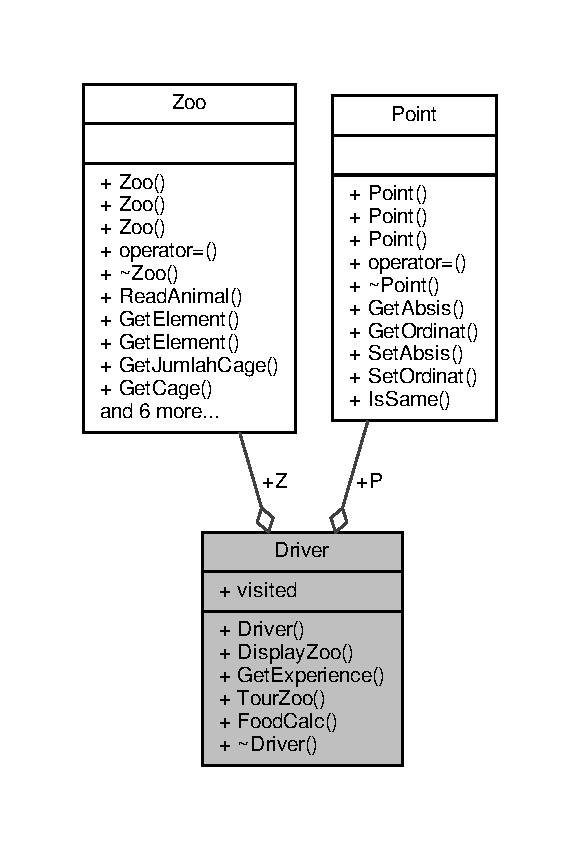
\includegraphics[height=550pt]{classDriver__coll__graph}
\end{center}
\end{figure}
\subsection*{Classes}
\begin{DoxyCompactItemize}
\item 
class \hyperlink{classDriver_1_1Kelas}{Kelas}
\end{DoxyCompactItemize}
\subsection*{Public Member Functions}
\begin{DoxyCompactItemize}
\item 
\hyperlink{classDriver_af0658d103e3e810a8e9ef0a53bb2e261}{Driver} ()
\begin{DoxyCompactList}\small\item\em Constructor. Menciptakan \hyperlink{classCage}{Cage} kosong tanpa animal. \end{DoxyCompactList}\item 
void \hyperlink{classDriver_aa8b4e139b99aad4720ce86286783dcdb}{Display\+Zoo} ()
\begin{DoxyCompactList}\small\item\em Display\+Zoo. Menampilkan zoo ke layar. \end{DoxyCompactList}\item 
void \hyperlink{classDriver_a2bc17a8251eab4cfdb7d74c7f7299c6e}{Get\+Experience} ()
\begin{DoxyCompactList}\small\item\em Get\+Experience. Mencetak ke layar eksperimen yang didapat pengunjung. \end{DoxyCompactList}\item 
void \hyperlink{classDriver_af3677b3b6adc2ccc5d486be1e4462fba}{Display\+Tour} ()
\begin{DoxyCompactList}\small\item\em Display\+Zoo. Menampilkan tur yang terjadi ke layar. \end{DoxyCompactList}\item 
void \hyperlink{classDriver_aa56ed0eaa789f78765708e15032d6534}{Tour\+Zoo} ()
\begin{DoxyCompactList}\small\item\em Tour\+Zoo. Melakukan tur zoo. \end{DoxyCompactList}\item 
float \hyperlink{classDriver_a0f85e40efd4983b0434307ca0647f378}{Food\+Calc} ()
\begin{DoxyCompactList}\small\item\em Food\+Calc. Melakukan perhitungan makanan yang harus disiapkan. \end{DoxyCompactList}\item 
\hyperlink{classDriver_ac7645eea8d3ce2bc39ddbda5e840297a}{$\sim$\+Driver} ()
\begin{DoxyCompactList}\small\item\em Destructor. \end{DoxyCompactList}\item 
void \hyperlink{classDriver_a56f5ca7386659854399999ffb6d8d043}{Display\+Menu} ()
\begin{DoxyCompactList}\small\item\em Display\+Menu. Menampilkan menu utama ke layar. \end{DoxyCompactList}\item 
\hyperlink{classZoo}{Zoo} \& \hyperlink{classDriver_a61680a5ffa5a314e4cb411b7bff29f26}{Get\+Zoo} ()
\begin{DoxyCompactList}\small\item\em Get\+Zoo. \end{DoxyCompactList}\item 
\hyperlink{classPoint}{Point} \& \hyperlink{classDriver_a5efd12ebb8faa45d7c95a23ed83ac5d5}{Get\+Point} ()
\begin{DoxyCompactList}\small\item\em Get\+Zoo. \end{DoxyCompactList}\end{DoxyCompactItemize}
\subsection*{Public Attributes}
\begin{DoxyCompactItemize}
\item 
\hyperlink{classZoo}{Zoo} \hyperlink{classDriver_a15f54a382cba3cdcf82c396cecfa3f9e}{Z}
\item 
bool $\ast$$\ast$ \hyperlink{classDriver_ab338d327140ab7a1a9469d5c16c2697f}{visited}
\item 
\hyperlink{classPoint}{Point} \hyperlink{classDriver_a967bca94eece374e66e7ed827f22cf51}{P}
\end{DoxyCompactItemize}


\subsection{Constructor \& Destructor Documentation}
\index{Driver@{Driver}!Driver@{Driver}}
\index{Driver@{Driver}!Driver@{Driver}}
\subsubsection[{\texorpdfstring{Driver()}{Driver()}}]{\setlength{\rightskip}{0pt plus 5cm}Driver\+::\+Driver (
\begin{DoxyParamCaption}
{}
\end{DoxyParamCaption}
)}\hypertarget{classDriver_af0658d103e3e810a8e9ef0a53bb2e261}{}\label{classDriver_af0658d103e3e810a8e9ef0a53bb2e261}


Constructor. Menciptakan \hyperlink{classCage}{Cage} kosong tanpa animal. 

\index{Driver@{Driver}!````~Driver@{$\sim$\+Driver}}
\index{````~Driver@{$\sim$\+Driver}!Driver@{Driver}}
\subsubsection[{\texorpdfstring{$\sim$\+Driver()}{~Driver()}}]{\setlength{\rightskip}{0pt plus 5cm}Driver\+::$\sim$\+Driver (
\begin{DoxyParamCaption}
{}
\end{DoxyParamCaption}
)\hspace{0.3cm}{\ttfamily [inline]}}\hypertarget{classDriver_ac7645eea8d3ce2bc39ddbda5e840297a}{}\label{classDriver_ac7645eea8d3ce2bc39ddbda5e840297a}


Destructor. 



\subsection{Member Function Documentation}
\index{Driver@{Driver}!Display\+Menu@{Display\+Menu}}
\index{Display\+Menu@{Display\+Menu}!Driver@{Driver}}
\subsubsection[{\texorpdfstring{Display\+Menu()}{DisplayMenu()}}]{\setlength{\rightskip}{0pt plus 5cm}void Driver\+::\+Display\+Menu (
\begin{DoxyParamCaption}
{}
\end{DoxyParamCaption}
)}\hypertarget{classDriver_a56f5ca7386659854399999ffb6d8d043}{}\label{classDriver_a56f5ca7386659854399999ffb6d8d043}


Display\+Menu. Menampilkan menu utama ke layar. 

\index{Driver@{Driver}!Display\+Tour@{Display\+Tour}}
\index{Display\+Tour@{Display\+Tour}!Driver@{Driver}}
\subsubsection[{\texorpdfstring{Display\+Tour()}{DisplayTour()}}]{\setlength{\rightskip}{0pt plus 5cm}void Driver\+::\+Display\+Tour (
\begin{DoxyParamCaption}
{}
\end{DoxyParamCaption}
)}\hypertarget{classDriver_af3677b3b6adc2ccc5d486be1e4462fba}{}\label{classDriver_af3677b3b6adc2ccc5d486be1e4462fba}


Display\+Zoo. Menampilkan tur yang terjadi ke layar. 

\index{Driver@{Driver}!Display\+Zoo@{Display\+Zoo}}
\index{Display\+Zoo@{Display\+Zoo}!Driver@{Driver}}
\subsubsection[{\texorpdfstring{Display\+Zoo()}{DisplayZoo()}}]{\setlength{\rightskip}{0pt plus 5cm}void Driver\+::\+Display\+Zoo (
\begin{DoxyParamCaption}
{}
\end{DoxyParamCaption}
)}\hypertarget{classDriver_aa8b4e139b99aad4720ce86286783dcdb}{}\label{classDriver_aa8b4e139b99aad4720ce86286783dcdb}


Display\+Zoo. Menampilkan zoo ke layar. 

\index{Driver@{Driver}!Food\+Calc@{Food\+Calc}}
\index{Food\+Calc@{Food\+Calc}!Driver@{Driver}}
\subsubsection[{\texorpdfstring{Food\+Calc()}{FoodCalc()}}]{\setlength{\rightskip}{0pt plus 5cm}float Driver\+::\+Food\+Calc (
\begin{DoxyParamCaption}
{}
\end{DoxyParamCaption}
)}\hypertarget{classDriver_a0f85e40efd4983b0434307ca0647f378}{}\label{classDriver_a0f85e40efd4983b0434307ca0647f378}


Food\+Calc. Melakukan perhitungan makanan yang harus disiapkan. 

\begin{DoxyReturn}{Returns}
Mengembalikan jumlah makanan yang harus disiapkan. 
\end{DoxyReturn}
\index{Driver@{Driver}!Get\+Experience@{Get\+Experience}}
\index{Get\+Experience@{Get\+Experience}!Driver@{Driver}}
\subsubsection[{\texorpdfstring{Get\+Experience()}{GetExperience()}}]{\setlength{\rightskip}{0pt plus 5cm}void Driver\+::\+Get\+Experience (
\begin{DoxyParamCaption}
{}
\end{DoxyParamCaption}
)}\hypertarget{classDriver_a2bc17a8251eab4cfdb7d74c7f7299c6e}{}\label{classDriver_a2bc17a8251eab4cfdb7d74c7f7299c6e}


Get\+Experience. Mencetak ke layar eksperimen yang didapat pengunjung. 

\index{Driver@{Driver}!Get\+Point@{Get\+Point}}
\index{Get\+Point@{Get\+Point}!Driver@{Driver}}
\subsubsection[{\texorpdfstring{Get\+Point()}{GetPoint()}}]{\setlength{\rightskip}{0pt plus 5cm}{\bf Point} \& Driver\+::\+Get\+Point (
\begin{DoxyParamCaption}
{}
\end{DoxyParamCaption}
)}\hypertarget{classDriver_a5efd12ebb8faa45d7c95a23ed83ac5d5}{}\label{classDriver_a5efd12ebb8faa45d7c95a23ed83ac5d5}


Get\+Zoo. 

\begin{DoxyReturn}{Returns}
Mengembalikan point. 
\end{DoxyReturn}
\index{Driver@{Driver}!Get\+Zoo@{Get\+Zoo}}
\index{Get\+Zoo@{Get\+Zoo}!Driver@{Driver}}
\subsubsection[{\texorpdfstring{Get\+Zoo()}{GetZoo()}}]{\setlength{\rightskip}{0pt plus 5cm}{\bf Zoo} \& Driver\+::\+Get\+Zoo (
\begin{DoxyParamCaption}
{}
\end{DoxyParamCaption}
)}\hypertarget{classDriver_a61680a5ffa5a314e4cb411b7bff29f26}{}\label{classDriver_a61680a5ffa5a314e4cb411b7bff29f26}


Get\+Zoo. 

\begin{DoxyReturn}{Returns}
Mengembalikan zoo. 
\end{DoxyReturn}
\index{Driver@{Driver}!Tour\+Zoo@{Tour\+Zoo}}
\index{Tour\+Zoo@{Tour\+Zoo}!Driver@{Driver}}
\subsubsection[{\texorpdfstring{Tour\+Zoo()}{TourZoo()}}]{\setlength{\rightskip}{0pt plus 5cm}void Driver\+::\+Tour\+Zoo (
\begin{DoxyParamCaption}
{}
\end{DoxyParamCaption}
)}\hypertarget{classDriver_aa56ed0eaa789f78765708e15032d6534}{}\label{classDriver_aa56ed0eaa789f78765708e15032d6534}


Tour\+Zoo. Melakukan tur zoo. 



\subsection{Member Data Documentation}
\index{Driver@{Driver}!P@{P}}
\index{P@{P}!Driver@{Driver}}
\subsubsection[{\texorpdfstring{P}{P}}]{\setlength{\rightskip}{0pt plus 5cm}{\bf Point} Driver\+::P}\hypertarget{classDriver_a967bca94eece374e66e7ed827f22cf51}{}\label{classDriver_a967bca94eece374e66e7ed827f22cf51}
\index{Driver@{Driver}!visited@{visited}}
\index{visited@{visited}!Driver@{Driver}}
\subsubsection[{\texorpdfstring{visited}{visited}}]{\setlength{\rightskip}{0pt plus 5cm}bool$\ast$$\ast$ Driver\+::visited}\hypertarget{classDriver_ab338d327140ab7a1a9469d5c16c2697f}{}\label{classDriver_ab338d327140ab7a1a9469d5c16c2697f}
\index{Driver@{Driver}!Z@{Z}}
\index{Z@{Z}!Driver@{Driver}}
\subsubsection[{\texorpdfstring{Z}{Z}}]{\setlength{\rightskip}{0pt plus 5cm}{\bf Zoo} Driver\+::Z}\hypertarget{classDriver_a15f54a382cba3cdcf82c396cecfa3f9e}{}\label{classDriver_a15f54a382cba3cdcf82c396cecfa3f9e}


The documentation for this class was generated from the following files\+:\begin{DoxyCompactItemize}
\item 
driver/\hyperlink{driver_8h}{driver.\+h}\item 
driver/\hyperlink{driver_8cpp}{driver.\+cpp}\end{DoxyCompactItemize}

\hypertarget{classDuck}{}\section{Duck Class Reference}
\label{classDuck}\index{Duck@{Duck}}


{\ttfamily \#include $<$duck.\+h$>$}



Inheritance diagram for Duck\+:
\nopagebreak
\begin{figure}[H]
\begin{center}
\leavevmode
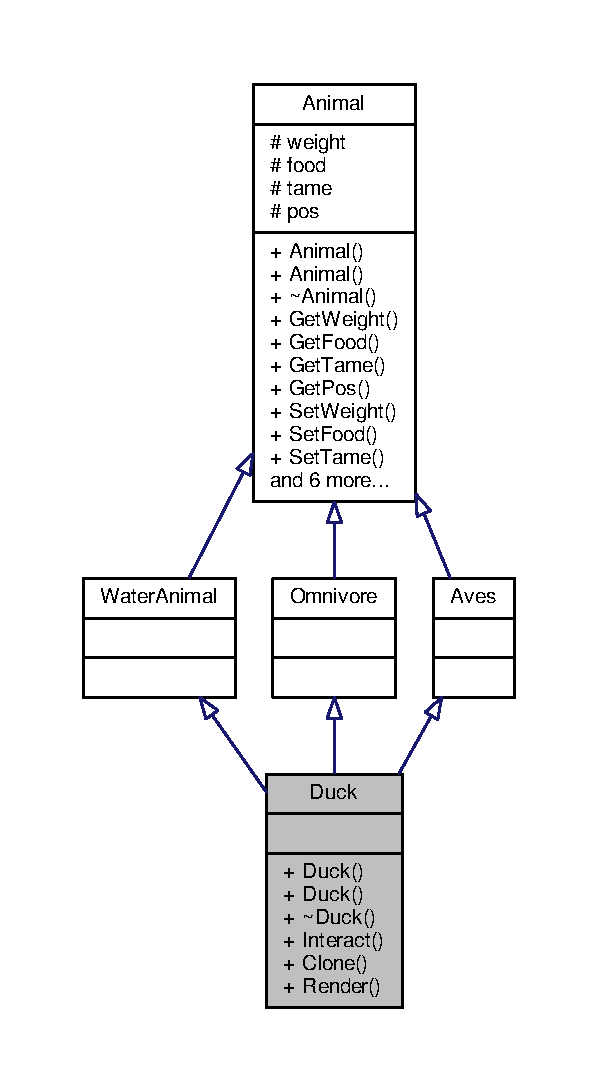
\includegraphics[width=210pt]{classDuck__inherit__graph}
\end{center}
\end{figure}


Collaboration diagram for Duck\+:
\nopagebreak
\begin{figure}[H]
\begin{center}
\leavevmode
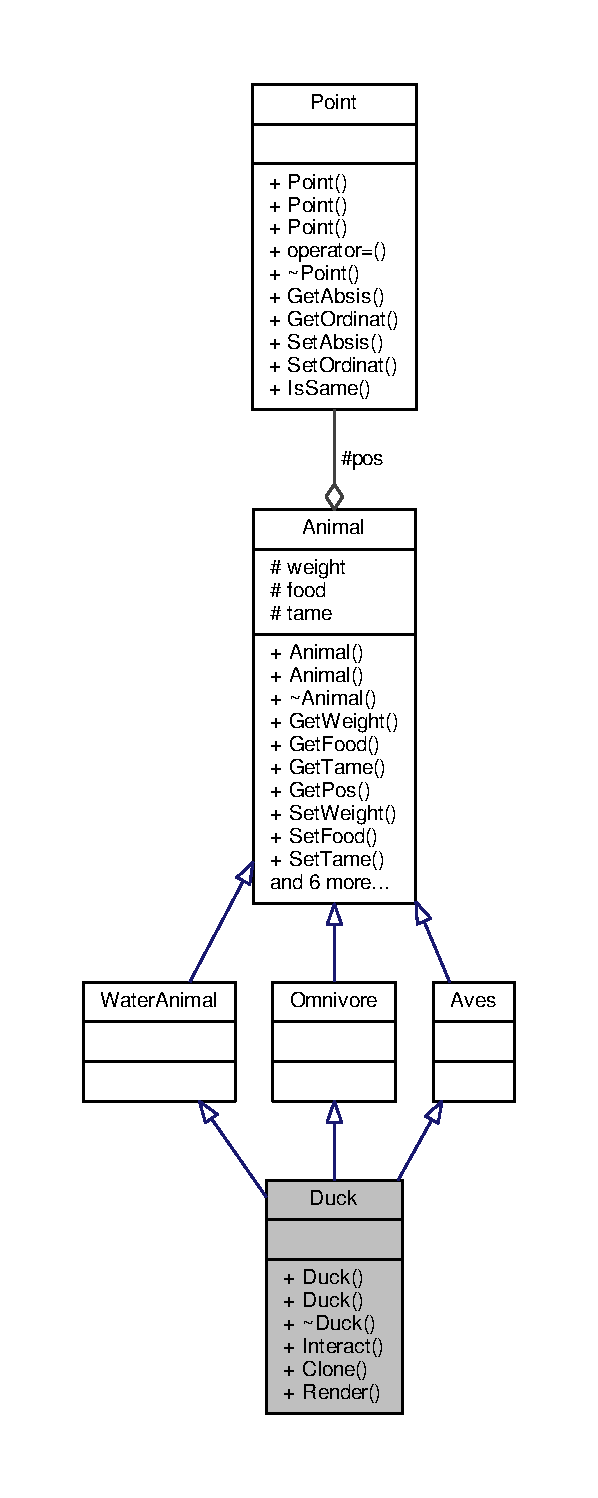
\includegraphics[height=550pt]{classDuck__coll__graph}
\end{center}
\end{figure}
\subsection*{Public Member Functions}
\begin{DoxyCompactItemize}
\item 
\hyperlink{classDuck_a65753b7b6eb80c4639f6bf165b8db9a6}{Duck} ()
\begin{DoxyCompactList}\small\item\em Constructor. Menciptakan objek \hyperlink{classDuck}{Duck}. \end{DoxyCompactList}\item 
virtual \hyperlink{classDuck_a073eb979ff45a938fde4cf769f5e579b}{$\sim$\+Duck} ()
\begin{DoxyCompactList}\small\item\em Destructor. \end{DoxyCompactList}\item 
string \hyperlink{classDuck_a9355aa821755703c02ac96e49692eaea}{Interact} ()
\begin{DoxyCompactList}\small\item\em Interaksi yang dilakukan \hyperlink{classDuck}{Duck}. \end{DoxyCompactList}\item 
virtual \hyperlink{classDuck}{Duck} $\ast$ \hyperlink{classDuck_ae3ff98b443c887f37ce63e3ed2e3a690}{Clone} () const 
\begin{DoxyCompactList}\small\item\em Melakukan cloning untuk menciptakan objek \hyperlink{classDuck}{Duck} baru. \end{DoxyCompactList}\item 
char \hyperlink{classDuck_a8453f95adcf2e7ff1b35a1a9d9948510}{Render} ()
\begin{DoxyCompactList}\small\item\em Render dari \hyperlink{classDuck}{Duck}. \end{DoxyCompactList}\end{DoxyCompactItemize}
\subsection*{Additional Inherited Members}


\subsection{Detailed Description}
Kelas \hyperlink{classDuck}{Duck} merupakan kelas untuk real object \hyperlink{classDuck}{Duck} 

\subsection{Constructor \& Destructor Documentation}
\index{Duck@{Duck}!Duck@{Duck}}
\index{Duck@{Duck}!Duck@{Duck}}
\subsubsection[{\texorpdfstring{Duck()}{Duck()}}]{\setlength{\rightskip}{0pt plus 5cm}Duck\+::\+Duck (
\begin{DoxyParamCaption}
{}
\end{DoxyParamCaption}
)\hspace{0.3cm}{\ttfamily [inline]}}\hypertarget{classDuck_a65753b7b6eb80c4639f6bf165b8db9a6}{}\label{classDuck_a65753b7b6eb80c4639f6bf165b8db9a6}


Constructor. Menciptakan objek \hyperlink{classDuck}{Duck}. 

\index{Duck@{Duck}!````~Duck@{$\sim$\+Duck}}
\index{````~Duck@{$\sim$\+Duck}!Duck@{Duck}}
\subsubsection[{\texorpdfstring{$\sim$\+Duck()}{~Duck()}}]{\setlength{\rightskip}{0pt plus 5cm}virtual Duck\+::$\sim$\+Duck (
\begin{DoxyParamCaption}
{}
\end{DoxyParamCaption}
)\hspace{0.3cm}{\ttfamily [inline]}, {\ttfamily [virtual]}}\hypertarget{classDuck_a073eb979ff45a938fde4cf769f5e579b}{}\label{classDuck_a073eb979ff45a938fde4cf769f5e579b}


Destructor. 



\subsection{Member Function Documentation}
\index{Duck@{Duck}!Clone@{Clone}}
\index{Clone@{Clone}!Duck@{Duck}}
\subsubsection[{\texorpdfstring{Clone() const }{Clone() const }}]{\setlength{\rightskip}{0pt plus 5cm}virtual {\bf Duck}$\ast$ Duck\+::\+Clone (
\begin{DoxyParamCaption}
{}
\end{DoxyParamCaption}
) const\hspace{0.3cm}{\ttfamily [inline]}, {\ttfamily [virtual]}}\hypertarget{classDuck_ae3ff98b443c887f37ce63e3ed2e3a690}{}\label{classDuck_ae3ff98b443c887f37ce63e3ed2e3a690}


Melakukan cloning untuk menciptakan objek \hyperlink{classDuck}{Duck} baru. 

\begin{DoxyReturn}{Returns}
Mengembalikan pointer to \hyperlink{classDuck}{Duck} objek tersebut. 
\end{DoxyReturn}


Implements \hyperlink{classAnimal_a3fc95e2a588b653b9b315e6c7a29c89f}{Animal}.

\index{Duck@{Duck}!Interact@{Interact}}
\index{Interact@{Interact}!Duck@{Duck}}
\subsubsection[{\texorpdfstring{Interact()}{Interact()}}]{\setlength{\rightskip}{0pt plus 5cm}string Duck\+::\+Interact (
\begin{DoxyParamCaption}
{}
\end{DoxyParamCaption}
)\hspace{0.3cm}{\ttfamily [inline]}, {\ttfamily [virtual]}}\hypertarget{classDuck_a9355aa821755703c02ac96e49692eaea}{}\label{classDuck_a9355aa821755703c02ac96e49692eaea}


Interaksi yang dilakukan \hyperlink{classDuck}{Duck}. 

\begin{DoxyReturn}{Returns}
Mengembalikan string yang merepresentasikan suara \hyperlink{classDuck}{Duck}. 
\end{DoxyReturn}


Implements \hyperlink{classAnimal_ad5a55fb0355a9425fee6611003d9892c}{Animal}.

\index{Duck@{Duck}!Render@{Render}}
\index{Render@{Render}!Duck@{Duck}}
\subsubsection[{\texorpdfstring{Render()}{Render()}}]{\setlength{\rightskip}{0pt plus 5cm}char Duck\+::\+Render (
\begin{DoxyParamCaption}
{}
\end{DoxyParamCaption}
)\hspace{0.3cm}{\ttfamily [inline]}, {\ttfamily [virtual]}}\hypertarget{classDuck_a8453f95adcf2e7ff1b35a1a9d9948510}{}\label{classDuck_a8453f95adcf2e7ff1b35a1a9d9948510}


Render dari \hyperlink{classDuck}{Duck}. 

\begin{DoxyReturn}{Returns}
Mengembalikan char yang merupakan representasi kode \hyperlink{classDuck}{Duck}. 
\end{DoxyReturn}


Implements \hyperlink{classAnimal_a43a47c0f41d211128e04abc6add53def}{Animal}.



The documentation for this class was generated from the following file\+:\begin{DoxyCompactItemize}
\item 
duck/\hyperlink{duck_8h}{duck.\+h}\end{DoxyCompactItemize}

\hypertarget{classDugong}{}\section{Dugong Class Reference}
\label{classDugong}\index{Dugong@{Dugong}}


{\ttfamily \#include $<$dugong.\+h$>$}



Inheritance diagram for Dugong\+:
\nopagebreak
\begin{figure}[H]
\begin{center}
\leavevmode
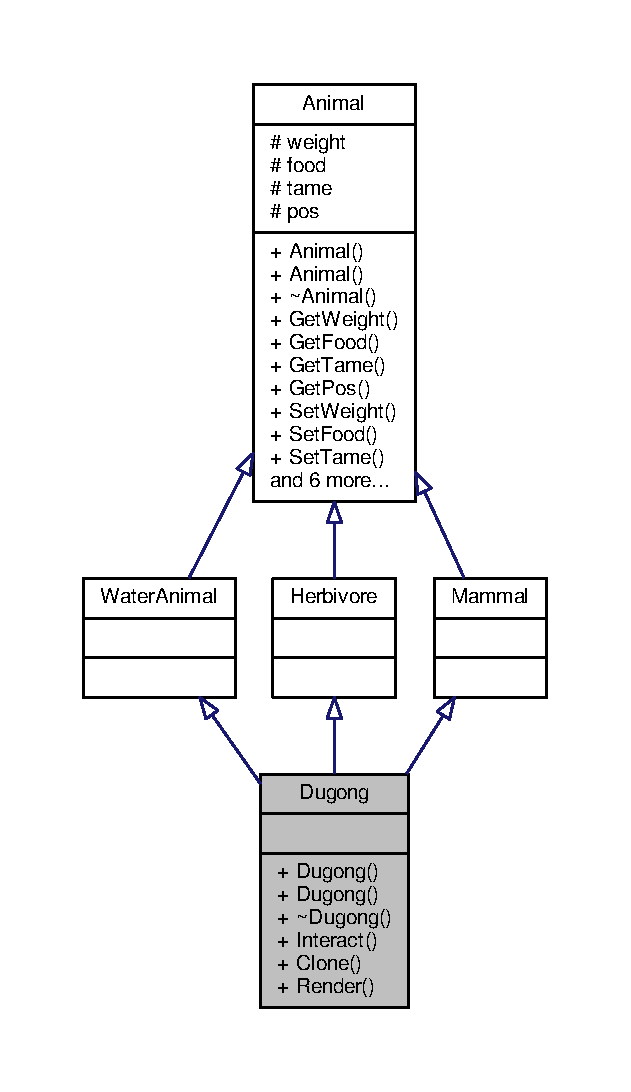
\includegraphics[width=303pt]{classDugong__inherit__graph}
\end{center}
\end{figure}


Collaboration diagram for Dugong\+:
\nopagebreak
\begin{figure}[H]
\begin{center}
\leavevmode
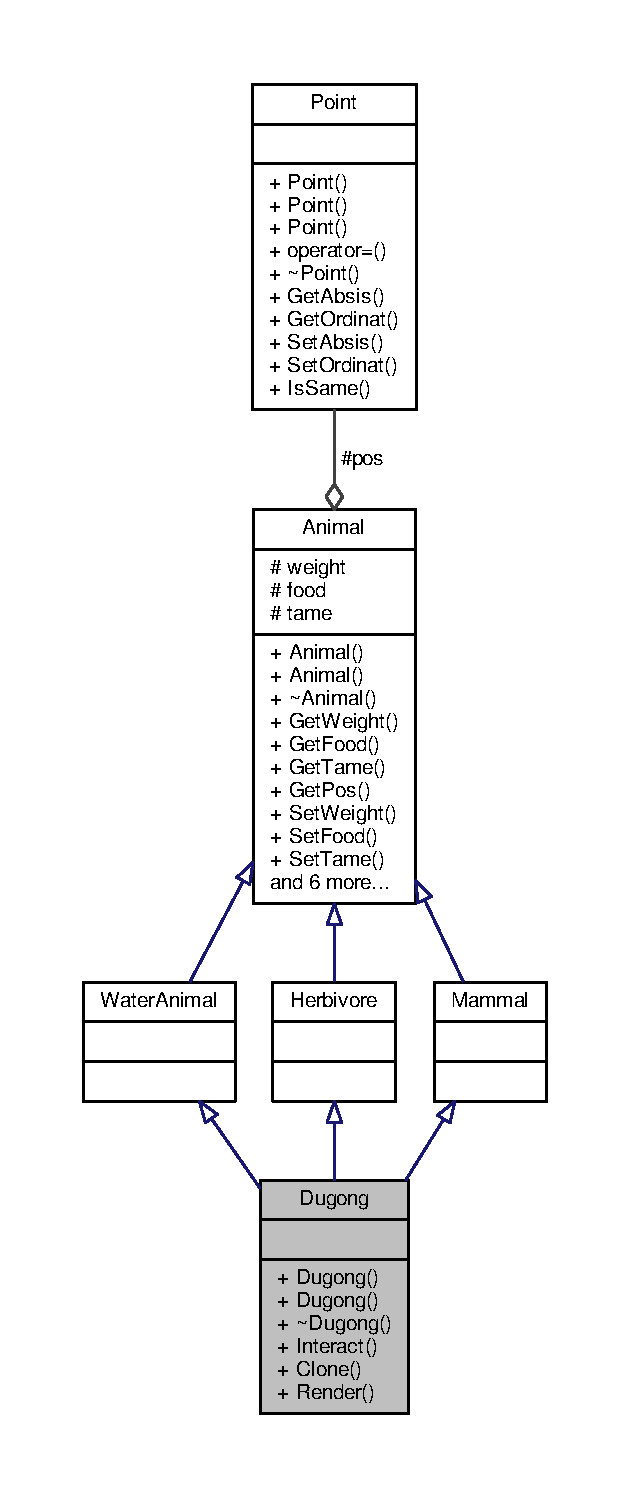
\includegraphics[height=550pt]{classDugong__coll__graph}
\end{center}
\end{figure}
\subsection*{Public Member Functions}
\begin{DoxyCompactItemize}
\item 
\hyperlink{classDugong_ab18a993807c0daa4b4a7eeaf7118ead7}{Dugong} ()
\begin{DoxyCompactList}\small\item\em Constructor. Menciptakan objek \hyperlink{classDugong}{Dugong}. \end{DoxyCompactList}\item 
\hyperlink{classDugong_af4aa8ab8370bbea5ccb75f5dd104f8e8}{Dugong} (float w, float f, bool t)
\begin{DoxyCompactList}\small\item\em Constructor dengan parameter. Menciptakan objek \hyperlink{classDugong}{Dugong} dengan berat w, jumlah makanan f, dan status jinak t. \end{DoxyCompactList}\item 
virtual \hyperlink{classDugong_a0fe188826a301ecf2b90f2eb60c9e5da}{$\sim$\+Dugong} ()
\begin{DoxyCompactList}\small\item\em Destructor. \end{DoxyCompactList}\item 
string \hyperlink{classDugong_a861c589c05a791faf03297eb6e718d9e}{Interact} ()
\begin{DoxyCompactList}\small\item\em Interaksi yang dilakukan \hyperlink{classDugong}{Dugong}. \end{DoxyCompactList}\item 
virtual \hyperlink{classDugong}{Dugong} $\ast$ \hyperlink{classDugong_a8209b4208bd32dfc0fa4e701679306c1}{Clone} () const 
\begin{DoxyCompactList}\small\item\em Melakukan cloning untuk menciptakan objek \hyperlink{classDugong}{Dugong} baru. \end{DoxyCompactList}\item 
char \hyperlink{classDugong_af82a8983c960604aa27dabe7fec53362}{Render} ()
\begin{DoxyCompactList}\small\item\em Render dari \hyperlink{classDugong}{Dugong}. \end{DoxyCompactList}\end{DoxyCompactItemize}
\subsection*{Additional Inherited Members}


\subsection{Detailed Description}
Kelas \hyperlink{classDugong}{Dugong} merupakan kelas untuk real object \hyperlink{classDugong}{Dugong} 

\subsection{Constructor \& Destructor Documentation}
\index{Dugong@{Dugong}!Dugong@{Dugong}}
\index{Dugong@{Dugong}!Dugong@{Dugong}}
\subsubsection[{\texorpdfstring{Dugong()}{Dugong()}}]{\setlength{\rightskip}{0pt plus 5cm}Dugong\+::\+Dugong (
\begin{DoxyParamCaption}
{}
\end{DoxyParamCaption}
)\hspace{0.3cm}{\ttfamily [inline]}}\hypertarget{classDugong_ab18a993807c0daa4b4a7eeaf7118ead7}{}\label{classDugong_ab18a993807c0daa4b4a7eeaf7118ead7}


Constructor. Menciptakan objek \hyperlink{classDugong}{Dugong}. 

\index{Dugong@{Dugong}!Dugong@{Dugong}}
\index{Dugong@{Dugong}!Dugong@{Dugong}}
\subsubsection[{\texorpdfstring{Dugong(float w, float f, bool t)}{Dugong(float w, float f, bool t)}}]{\setlength{\rightskip}{0pt plus 5cm}Dugong\+::\+Dugong (
\begin{DoxyParamCaption}
\item[{float}]{w, }
\item[{float}]{f, }
\item[{bool}]{t}
\end{DoxyParamCaption}
)\hspace{0.3cm}{\ttfamily [inline]}}\hypertarget{classDugong_af4aa8ab8370bbea5ccb75f5dd104f8e8}{}\label{classDugong_af4aa8ab8370bbea5ccb75f5dd104f8e8}


Constructor dengan parameter. Menciptakan objek \hyperlink{classDugong}{Dugong} dengan berat w, jumlah makanan f, dan status jinak t. 


\begin{DoxyParams}{Parameters}
{\em w} & Berat \hyperlink{classDugong}{Dugong}. \\
\hline
{\em k} & Jumlah makanan \hyperlink{classDugong}{Dugong}. \\
\hline
{\em t} & Status jinak \hyperlink{classDugong}{Dugong}. \\
\hline
\end{DoxyParams}
\index{Dugong@{Dugong}!````~Dugong@{$\sim$\+Dugong}}
\index{````~Dugong@{$\sim$\+Dugong}!Dugong@{Dugong}}
\subsubsection[{\texorpdfstring{$\sim$\+Dugong()}{~Dugong()}}]{\setlength{\rightskip}{0pt plus 5cm}virtual Dugong\+::$\sim$\+Dugong (
\begin{DoxyParamCaption}
{}
\end{DoxyParamCaption}
)\hspace{0.3cm}{\ttfamily [inline]}, {\ttfamily [virtual]}}\hypertarget{classDugong_a0fe188826a301ecf2b90f2eb60c9e5da}{}\label{classDugong_a0fe188826a301ecf2b90f2eb60c9e5da}


Destructor. 



\subsection{Member Function Documentation}
\index{Dugong@{Dugong}!Clone@{Clone}}
\index{Clone@{Clone}!Dugong@{Dugong}}
\subsubsection[{\texorpdfstring{Clone() const }{Clone() const }}]{\setlength{\rightskip}{0pt plus 5cm}virtual {\bf Dugong}$\ast$ Dugong\+::\+Clone (
\begin{DoxyParamCaption}
{}
\end{DoxyParamCaption}
) const\hspace{0.3cm}{\ttfamily [inline]}, {\ttfamily [virtual]}}\hypertarget{classDugong_a8209b4208bd32dfc0fa4e701679306c1}{}\label{classDugong_a8209b4208bd32dfc0fa4e701679306c1}


Melakukan cloning untuk menciptakan objek \hyperlink{classDugong}{Dugong} baru. 

\begin{DoxyReturn}{Returns}
Mengembalikan pointer to \hyperlink{classDugong}{Dugong} objek tersebut. 
\end{DoxyReturn}


Implements \hyperlink{classAnimal_a3fc95e2a588b653b9b315e6c7a29c89f}{Animal}.

\index{Dugong@{Dugong}!Interact@{Interact}}
\index{Interact@{Interact}!Dugong@{Dugong}}
\subsubsection[{\texorpdfstring{Interact()}{Interact()}}]{\setlength{\rightskip}{0pt plus 5cm}string Dugong\+::\+Interact (
\begin{DoxyParamCaption}
{}
\end{DoxyParamCaption}
)\hspace{0.3cm}{\ttfamily [inline]}, {\ttfamily [virtual]}}\hypertarget{classDugong_a861c589c05a791faf03297eb6e718d9e}{}\label{classDugong_a861c589c05a791faf03297eb6e718d9e}


Interaksi yang dilakukan \hyperlink{classDugong}{Dugong}. 

\begin{DoxyReturn}{Returns}
Mengembalikan string yang merepresentasikan suara \hyperlink{classDugong}{Dugong}. 
\end{DoxyReturn}


Implements \hyperlink{classAnimal_ad5a55fb0355a9425fee6611003d9892c}{Animal}.

\index{Dugong@{Dugong}!Render@{Render}}
\index{Render@{Render}!Dugong@{Dugong}}
\subsubsection[{\texorpdfstring{Render()}{Render()}}]{\setlength{\rightskip}{0pt plus 5cm}char Dugong\+::\+Render (
\begin{DoxyParamCaption}
{}
\end{DoxyParamCaption}
)\hspace{0.3cm}{\ttfamily [inline]}, {\ttfamily [virtual]}}\hypertarget{classDugong_af82a8983c960604aa27dabe7fec53362}{}\label{classDugong_af82a8983c960604aa27dabe7fec53362}


Render dari \hyperlink{classDugong}{Dugong}. 

\begin{DoxyReturn}{Returns}
Mengembalikan char yang merupakan representasi kode \hyperlink{classDugong}{Dugong}. 
\end{DoxyReturn}


Implements \hyperlink{classAnimal_a43a47c0f41d211128e04abc6add53def}{Animal}.



The documentation for this class was generated from the following file\+:\begin{DoxyCompactItemize}
\item 
dugong/\hyperlink{dugong_8h}{dugong.\+h}\end{DoxyCompactItemize}

\hypertarget{classEagle}{}\section{Eagle Class Reference}
\label{classEagle}\index{Eagle@{Eagle}}


{\ttfamily \#include $<$eagle.\+h$>$}



Inheritance diagram for Eagle\+:
% FIG 0


Collaboration diagram for Eagle\+:
% FIG 1
\subsection*{Public Member Functions}
\begin{DoxyCompactItemize}
\item 
\hyperlink{classEagle_a8b205e5b26bece07d18b852b042851fe}{Eagle} ()
\begin{DoxyCompactList}\small\item\em Constructor. Menciptakan objek \hyperlink{classEagle}{Eagle}. \end{DoxyCompactList}\item 
\hyperlink{classEagle_ae59cc80952be37499b10e270714af1d8}{Eagle} (float w, float f, bool t)
\begin{DoxyCompactList}\small\item\em Constructor dengan parameter. Menciptakan objek \hyperlink{classEagle}{Eagle} dengan berat w, jumlah makanan f, dan status jinak t. \end{DoxyCompactList}\item 
virtual \hyperlink{classEagle_a530318b3eb744ad26c9060d61aa314fe}{$\sim$\+Eagle} ()
\begin{DoxyCompactList}\small\item\em Destructor. \end{DoxyCompactList}\item 
string \hyperlink{classEagle_a64abae4f80bcdcba7dac9f03126f42aa}{Interact} ()
\begin{DoxyCompactList}\small\item\em Interaksi yang dilakukan \hyperlink{classEagle}{Eagle}. \end{DoxyCompactList}\item 
virtual \hyperlink{classEagle}{Eagle} $\ast$ \hyperlink{classEagle_ace8cb419354688615938d2a53d5c1566}{Clone} () const 
\begin{DoxyCompactList}\small\item\em Melakukan cloning untuk menciptakan objek \hyperlink{classEagle}{Eagle} baru. \end{DoxyCompactList}\item 
char \hyperlink{classEagle_a34e512cb19b5ba1f8a7bce937c57f33f}{Render} ()
\begin{DoxyCompactList}\small\item\em Render dari \hyperlink{classEagle}{Eagle}. \end{DoxyCompactList}\end{DoxyCompactItemize}
\subsection*{Additional Inherited Members}


\subsection{Detailed Description}
Kelas \hyperlink{classEagle}{Eagle} merupakan kelas untuk real object \hyperlink{classEagle}{Eagle} 

\subsection{Constructor \& Destructor Documentation}
\index{Eagle@{Eagle}!Eagle@{Eagle}}
\index{Eagle@{Eagle}!Eagle@{Eagle}}
\subsubsection[{\texorpdfstring{Eagle()}{Eagle()}}]{\setlength{\rightskip}{0pt plus 5cm}Eagle\+::\+Eagle (
\begin{DoxyParamCaption}
{}
\end{DoxyParamCaption}
)\hspace{0.3cm}{\ttfamily [inline]}}\hypertarget{classEagle_a8b205e5b26bece07d18b852b042851fe}{}\label{classEagle_a8b205e5b26bece07d18b852b042851fe}


Constructor. Menciptakan objek \hyperlink{classEagle}{Eagle}. 

\index{Eagle@{Eagle}!Eagle@{Eagle}}
\index{Eagle@{Eagle}!Eagle@{Eagle}}
\subsubsection[{\texorpdfstring{Eagle(float w, float f, bool t)}{Eagle(float w, float f, bool t)}}]{\setlength{\rightskip}{0pt plus 5cm}Eagle\+::\+Eagle (
\begin{DoxyParamCaption}
\item[{float}]{w, }
\item[{float}]{f, }
\item[{bool}]{t}
\end{DoxyParamCaption}
)\hspace{0.3cm}{\ttfamily [inline]}}\hypertarget{classEagle_ae59cc80952be37499b10e270714af1d8}{}\label{classEagle_ae59cc80952be37499b10e270714af1d8}


Constructor dengan parameter. Menciptakan objek \hyperlink{classEagle}{Eagle} dengan berat w, jumlah makanan f, dan status jinak t. 


\begin{DoxyParams}{Parameters}
{\em w} & Berat \hyperlink{classEagle}{Eagle}. \\
\hline
{\em k} & Jumlah makanan \hyperlink{classEagle}{Eagle}. \\
\hline
{\em t} & Status jinak \hyperlink{classEagle}{Eagle}. \\
\hline
\end{DoxyParams}
\index{Eagle@{Eagle}!````~Eagle@{$\sim$\+Eagle}}
\index{````~Eagle@{$\sim$\+Eagle}!Eagle@{Eagle}}
\subsubsection[{\texorpdfstring{$\sim$\+Eagle()}{~Eagle()}}]{\setlength{\rightskip}{0pt plus 5cm}virtual Eagle\+::$\sim$\+Eagle (
\begin{DoxyParamCaption}
{}
\end{DoxyParamCaption}
)\hspace{0.3cm}{\ttfamily [inline]}, {\ttfamily [virtual]}}\hypertarget{classEagle_a530318b3eb744ad26c9060d61aa314fe}{}\label{classEagle_a530318b3eb744ad26c9060d61aa314fe}


Destructor. 



\subsection{Member Function Documentation}
\index{Eagle@{Eagle}!Clone@{Clone}}
\index{Clone@{Clone}!Eagle@{Eagle}}
\subsubsection[{\texorpdfstring{Clone() const }{Clone() const }}]{\setlength{\rightskip}{0pt plus 5cm}virtual {\bf Eagle}$\ast$ Eagle\+::\+Clone (
\begin{DoxyParamCaption}
{}
\end{DoxyParamCaption}
) const\hspace{0.3cm}{\ttfamily [inline]}, {\ttfamily [virtual]}}\hypertarget{classEagle_ace8cb419354688615938d2a53d5c1566}{}\label{classEagle_ace8cb419354688615938d2a53d5c1566}


Melakukan cloning untuk menciptakan objek \hyperlink{classEagle}{Eagle} baru. 

\begin{DoxyReturn}{Returns}
Mengembalikan pointer to \hyperlink{classEagle}{Eagle} objek tersebut. 
\end{DoxyReturn}


Implements \hyperlink{classAnimal_a3fc95e2a588b653b9b315e6c7a29c89f}{Animal}.

\index{Eagle@{Eagle}!Interact@{Interact}}
\index{Interact@{Interact}!Eagle@{Eagle}}
\subsubsection[{\texorpdfstring{Interact()}{Interact()}}]{\setlength{\rightskip}{0pt plus 5cm}string Eagle\+::\+Interact (
\begin{DoxyParamCaption}
{}
\end{DoxyParamCaption}
)\hspace{0.3cm}{\ttfamily [inline]}, {\ttfamily [virtual]}}\hypertarget{classEagle_a64abae4f80bcdcba7dac9f03126f42aa}{}\label{classEagle_a64abae4f80bcdcba7dac9f03126f42aa}


Interaksi yang dilakukan \hyperlink{classEagle}{Eagle}. 

\begin{DoxyReturn}{Returns}
Mengembalikan string yang merepresentasikan suara \hyperlink{classEagle}{Eagle}. 
\end{DoxyReturn}


Implements \hyperlink{classAnimal_ad5a55fb0355a9425fee6611003d9892c}{Animal}.

\index{Eagle@{Eagle}!Render@{Render}}
\index{Render@{Render}!Eagle@{Eagle}}
\subsubsection[{\texorpdfstring{Render()}{Render()}}]{\setlength{\rightskip}{0pt plus 5cm}char Eagle\+::\+Render (
\begin{DoxyParamCaption}
{}
\end{DoxyParamCaption}
)\hspace{0.3cm}{\ttfamily [inline]}, {\ttfamily [virtual]}}\hypertarget{classEagle_a34e512cb19b5ba1f8a7bce937c57f33f}{}\label{classEagle_a34e512cb19b5ba1f8a7bce937c57f33f}


Render dari \hyperlink{classEagle}{Eagle}. 

\begin{DoxyReturn}{Returns}
Mengembalikan char yang merupakan representasi kode \hyperlink{classEagle}{Eagle}. 
\end{DoxyReturn}


Implements \hyperlink{classAnimal_a43a47c0f41d211128e04abc6add53def}{Animal}.



The documentation for this class was generated from the following file\+:\begin{DoxyCompactItemize}
\item 
eagle/\hyperlink{eagle_8h}{eagle.\+h}\end{DoxyCompactItemize}

\hypertarget{classElephant}{}\section{Elephant Class Reference}
\label{classElephant}\index{Elephant@{Elephant}}


{\ttfamily \#include $<$elephant.\+h$>$}



Inheritance diagram for Elephant\+:
\nopagebreak
\begin{figure}[H]
\begin{center}
\leavevmode
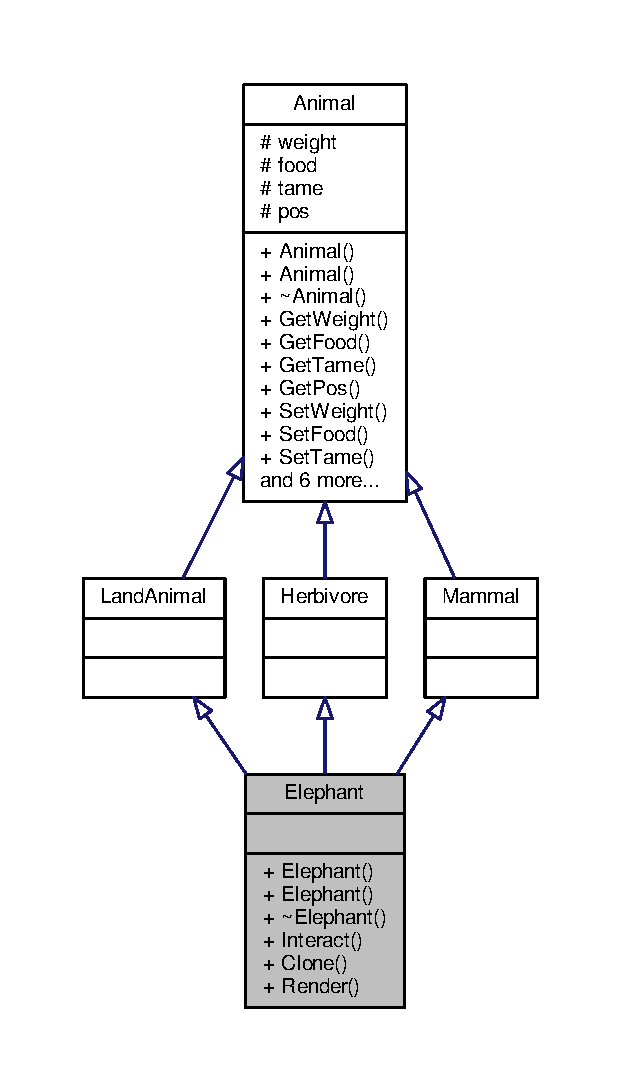
\includegraphics[width=298pt]{classElephant__inherit__graph}
\end{center}
\end{figure}


Collaboration diagram for Elephant\+:
\nopagebreak
\begin{figure}[H]
\begin{center}
\leavevmode
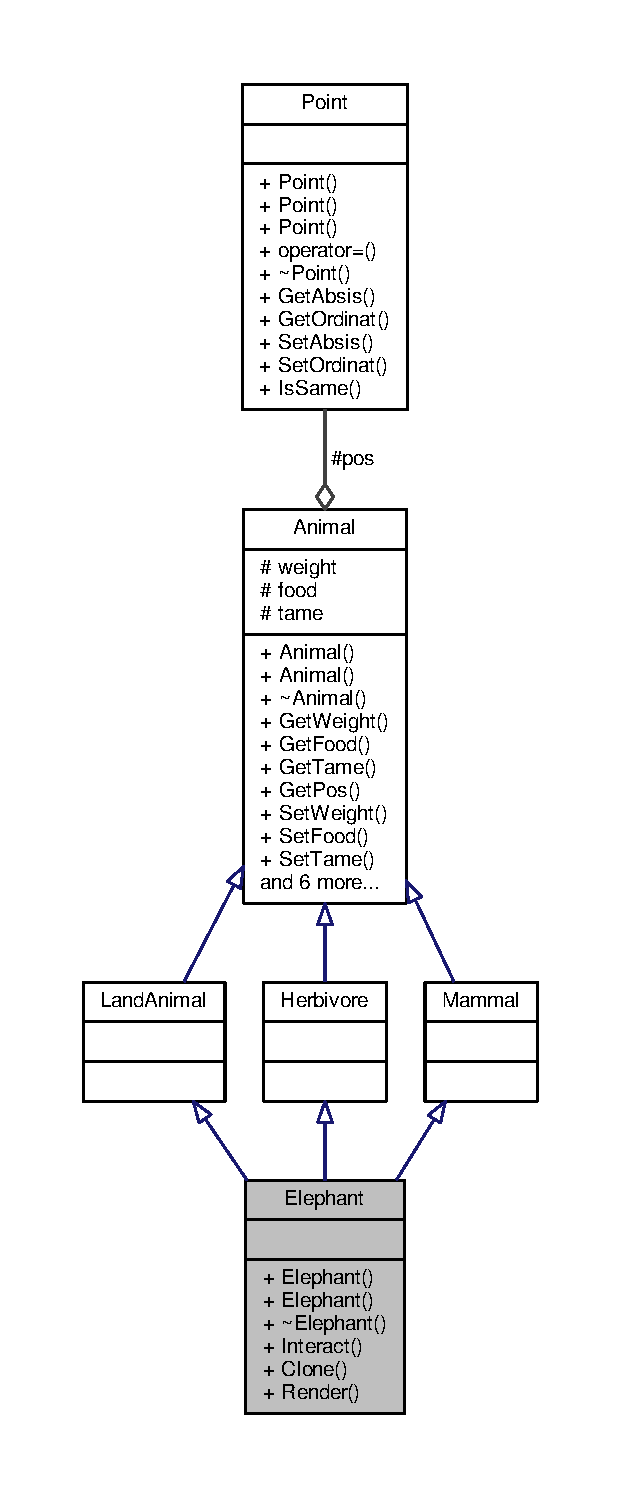
\includegraphics[height=550pt]{classElephant__coll__graph}
\end{center}
\end{figure}
\subsection*{Public Member Functions}
\begin{DoxyCompactItemize}
\item 
\hyperlink{classElephant_a372cc81064310f2f96db175b747647cb}{Elephant} ()
\begin{DoxyCompactList}\small\item\em Constructor. Menciptakan objek \hyperlink{classElephant}{Elephant}. \end{DoxyCompactList}\item 
\hyperlink{classElephant_a76bf83d1aacd5ff494532e14cf2a3bee}{Elephant} (float w, float f, bool t)
\begin{DoxyCompactList}\small\item\em Constructor dengan parameter. Menciptakan objek \hyperlink{classElephant}{Elephant} dengan berat w, jumlah makanan f, dan status jinak t. \end{DoxyCompactList}\item 
virtual \hyperlink{classElephant_aed5fb7142a24a101330af52652909075}{$\sim$\+Elephant} ()
\begin{DoxyCompactList}\small\item\em Destructor. \end{DoxyCompactList}\item 
string \hyperlink{classElephant_a4f2c4bef5ec886019ee88ad575f94fa7}{Interact} ()
\begin{DoxyCompactList}\small\item\em interact \end{DoxyCompactList}\item 
virtual \hyperlink{classElephant}{Elephant} $\ast$ \hyperlink{classElephant_a723a7c90f44a95d9886163e605aecea7}{Clone} () const 
\begin{DoxyCompactList}\small\item\em Melakukan cloning untuk menciptakan objek \hyperlink{classElephant}{Elephant} baru. \end{DoxyCompactList}\item 
char \hyperlink{classElephant_a7e412f36e1f88cd278dea76d4f383e95}{Render} ()
\begin{DoxyCompactList}\small\item\em render \end{DoxyCompactList}\end{DoxyCompactItemize}
\subsection*{Additional Inherited Members}


\subsection{Detailed Description}
Kelas \hyperlink{classElephant}{Elephant} merupakan kelas untuk real object \hyperlink{classElephant}{Elephant} 

\subsection{Constructor \& Destructor Documentation}
\index{Elephant@{Elephant}!Elephant@{Elephant}}
\index{Elephant@{Elephant}!Elephant@{Elephant}}
\subsubsection[{\texorpdfstring{Elephant()}{Elephant()}}]{\setlength{\rightskip}{0pt plus 5cm}Elephant\+::\+Elephant (
\begin{DoxyParamCaption}
{}
\end{DoxyParamCaption}
)\hspace{0.3cm}{\ttfamily [inline]}}\hypertarget{classElephant_a372cc81064310f2f96db175b747647cb}{}\label{classElephant_a372cc81064310f2f96db175b747647cb}


Constructor. Menciptakan objek \hyperlink{classElephant}{Elephant}. 

\index{Elephant@{Elephant}!Elephant@{Elephant}}
\index{Elephant@{Elephant}!Elephant@{Elephant}}
\subsubsection[{\texorpdfstring{Elephant(float w, float f, bool t)}{Elephant(float w, float f, bool t)}}]{\setlength{\rightskip}{0pt plus 5cm}Elephant\+::\+Elephant (
\begin{DoxyParamCaption}
\item[{float}]{w, }
\item[{float}]{f, }
\item[{bool}]{t}
\end{DoxyParamCaption}
)\hspace{0.3cm}{\ttfamily [inline]}}\hypertarget{classElephant_a76bf83d1aacd5ff494532e14cf2a3bee}{}\label{classElephant_a76bf83d1aacd5ff494532e14cf2a3bee}


Constructor dengan parameter. Menciptakan objek \hyperlink{classElephant}{Elephant} dengan berat w, jumlah makanan f, dan status jinak t. 


\begin{DoxyParams}{Parameters}
{\em w} & Berat \hyperlink{classElephant}{Elephant}. \\
\hline
{\em f} & Jumlah makanan \hyperlink{classElephant}{Elephant}. \\
\hline
{\em t} & Status jinak \hyperlink{classElephant}{Elephant}. \\
\hline
\end{DoxyParams}
\index{Elephant@{Elephant}!````~Elephant@{$\sim$\+Elephant}}
\index{````~Elephant@{$\sim$\+Elephant}!Elephant@{Elephant}}
\subsubsection[{\texorpdfstring{$\sim$\+Elephant()}{~Elephant()}}]{\setlength{\rightskip}{0pt plus 5cm}virtual Elephant\+::$\sim$\+Elephant (
\begin{DoxyParamCaption}
{}
\end{DoxyParamCaption}
)\hspace{0.3cm}{\ttfamily [inline]}, {\ttfamily [virtual]}}\hypertarget{classElephant_aed5fb7142a24a101330af52652909075}{}\label{classElephant_aed5fb7142a24a101330af52652909075}


Destructor. 



\subsection{Member Function Documentation}
\index{Elephant@{Elephant}!Clone@{Clone}}
\index{Clone@{Clone}!Elephant@{Elephant}}
\subsubsection[{\texorpdfstring{Clone() const }{Clone() const }}]{\setlength{\rightskip}{0pt plus 5cm}virtual {\bf Elephant}$\ast$ Elephant\+::\+Clone (
\begin{DoxyParamCaption}
{}
\end{DoxyParamCaption}
) const\hspace{0.3cm}{\ttfamily [inline]}, {\ttfamily [virtual]}}\hypertarget{classElephant_a723a7c90f44a95d9886163e605aecea7}{}\label{classElephant_a723a7c90f44a95d9886163e605aecea7}


Melakukan cloning untuk menciptakan objek \hyperlink{classElephant}{Elephant} baru. 

\begin{DoxyReturn}{Returns}
Mengembalikan pointer to \hyperlink{classElephant}{Elephant} objek tersebut. 
\end{DoxyReturn}


Implements \hyperlink{classAnimal_a3fc95e2a588b653b9b315e6c7a29c89f}{Animal}.

\index{Elephant@{Elephant}!Interact@{Interact}}
\index{Interact@{Interact}!Elephant@{Elephant}}
\subsubsection[{\texorpdfstring{Interact()}{Interact()}}]{\setlength{\rightskip}{0pt plus 5cm}string Elephant\+::\+Interact (
\begin{DoxyParamCaption}
{}
\end{DoxyParamCaption}
)\hspace{0.3cm}{\ttfamily [inline]}, {\ttfamily [virtual]}}\hypertarget{classElephant_a4f2c4bef5ec886019ee88ad575f94fa7}{}\label{classElephant_a4f2c4bef5ec886019ee88ad575f94fa7}


interact 

\begin{DoxyReturn}{Returns}
Mengembalikan string yang merepresentasikan suara \hyperlink{classElephant}{Elephant}. 
\end{DoxyReturn}


Implements \hyperlink{classAnimal_ad5a55fb0355a9425fee6611003d9892c}{Animal}.

\index{Elephant@{Elephant}!Render@{Render}}
\index{Render@{Render}!Elephant@{Elephant}}
\subsubsection[{\texorpdfstring{Render()}{Render()}}]{\setlength{\rightskip}{0pt plus 5cm}char Elephant\+::\+Render (
\begin{DoxyParamCaption}
{}
\end{DoxyParamCaption}
)\hspace{0.3cm}{\ttfamily [inline]}, {\ttfamily [virtual]}}\hypertarget{classElephant_a7e412f36e1f88cd278dea76d4f383e95}{}\label{classElephant_a7e412f36e1f88cd278dea76d4f383e95}


render 

\begin{DoxyReturn}{Returns}
Mengembalikan char yang merupakan representasi kode \hyperlink{classElephant}{Elephant}. 
\end{DoxyReturn}


Implements \hyperlink{classAnimal_a43a47c0f41d211128e04abc6add53def}{Animal}.



The documentation for this class was generated from the following file\+:\begin{DoxyCompactItemize}
\item 
\hyperlink{elephant_8h}{elephant.\+h}\end{DoxyCompactItemize}

\hypertarget{classEntrance}{}\section{Entrance Class Reference}
\label{classEntrance}\index{Entrance@{Entrance}}


{\ttfamily \#include $<$entrance.\+h$>$}



Inheritance diagram for Entrance\+:
% FIG 0


Collaboration diagram for Entrance\+:
% FIG 1
\subsection*{Public Member Functions}
\begin{DoxyCompactItemize}
\item 
char \hyperlink{classEntrance_a7226e0cd3d04f8370ede2573bc2852f3}{Render} ()
\begin{DoxyCompactList}\small\item\em Render dari \hyperlink{classEntrance}{Entrance}. \end{DoxyCompactList}\item 
virtual \hyperlink{classEntrance}{Entrance} $\ast$ \hyperlink{classEntrance_a360c7c24284c6004fcdacb09afa0d8ac}{Clone} () const 
\begin{DoxyCompactList}\small\item\em Melakukan cloning untuk menciptakan objek \hyperlink{classEntrance}{Entrance} baru. \end{DoxyCompactList}\end{DoxyCompactItemize}
\subsection*{Additional Inherited Members}


\subsection{Detailed Description}
Kelas \hyperlink{classEntrance}{Entrance} melambangkan jalan yang merupakan jalan masuk 

\subsection{Member Function Documentation}
\index{Entrance@{Entrance}!Clone@{Clone}}
\index{Clone@{Clone}!Entrance@{Entrance}}
\subsubsection[{\texorpdfstring{Clone() const }{Clone() const }}]{\setlength{\rightskip}{0pt plus 5cm}virtual {\bf Entrance}$\ast$ Entrance\+::\+Clone (
\begin{DoxyParamCaption}
{}
\end{DoxyParamCaption}
) const\hspace{0.3cm}{\ttfamily [inline]}, {\ttfamily [virtual]}}\hypertarget{classEntrance_a360c7c24284c6004fcdacb09afa0d8ac}{}\label{classEntrance_a360c7c24284c6004fcdacb09afa0d8ac}


Melakukan cloning untuk menciptakan objek \hyperlink{classEntrance}{Entrance} baru. 

\begin{DoxyReturn}{Returns}
Mengembalikan pointer to \hyperlink{classEntrance}{Entrance} objek tersebut. 
\end{DoxyReturn}


Reimplemented from \hyperlink{classRoad_a23ca807031dc27cb76d16a808e08beb7}{Road}.

\index{Entrance@{Entrance}!Render@{Render}}
\index{Render@{Render}!Entrance@{Entrance}}
\subsubsection[{\texorpdfstring{Render()}{Render()}}]{\setlength{\rightskip}{0pt plus 5cm}char Entrance\+::\+Render (
\begin{DoxyParamCaption}
{}
\end{DoxyParamCaption}
)\hspace{0.3cm}{\ttfamily [inline]}, {\ttfamily [virtual]}}\hypertarget{classEntrance_a7226e0cd3d04f8370ede2573bc2852f3}{}\label{classEntrance_a7226e0cd3d04f8370ede2573bc2852f3}


Render dari \hyperlink{classEntrance}{Entrance}. 

\begin{DoxyReturn}{Returns}
Mengembalikan char yang merupakan representasi kode \hyperlink{classEntrance}{Entrance}. 
\end{DoxyReturn}


Reimplemented from \hyperlink{classRoad_a72268486a71718b5b7957b63ecd565bc}{Road}.



The documentation for this class was generated from the following file\+:\begin{DoxyCompactItemize}
\item 
entrance/\hyperlink{entrance_8h}{entrance.\+h}\end{DoxyCompactItemize}

\hypertarget{classExit}{}\section{Exit Class Reference}
\label{classExit}\index{Exit@{Exit}}


{\ttfamily \#include $<$exit.\+h$>$}



Inheritance diagram for Exit\+:
% FIG 0


Collaboration diagram for Exit\+:
% FIG 1
\subsection*{Public Member Functions}
\begin{DoxyCompactItemize}
\item 
char \hyperlink{classExit_a9239e8b13c101d1aee8fde738e8a5fdc}{Render} ()
\begin{DoxyCompactList}\small\item\em Render dari \hyperlink{classExit}{Exit}. \end{DoxyCompactList}\item 
virtual \hyperlink{classExit}{Exit} $\ast$ \hyperlink{classExit_a827f84ddccdd30e9db0ed6918560d8d4}{Clone} () const 
\begin{DoxyCompactList}\small\item\em Melakukan cloning untuk menciptakan objek \hyperlink{classExit}{Exit} baru. \end{DoxyCompactList}\end{DoxyCompactItemize}
\subsection*{Additional Inherited Members}


\subsection{Detailed Description}
Kelas \hyperlink{classExit}{Exit} melambangkan jalan yang merupakan jalan keluar 

\subsection{Member Function Documentation}
\index{Exit@{Exit}!Clone@{Clone}}
\index{Clone@{Clone}!Exit@{Exit}}
\subsubsection[{\texorpdfstring{Clone() const }{Clone() const }}]{\setlength{\rightskip}{0pt plus 5cm}virtual {\bf Exit}$\ast$ Exit\+::\+Clone (
\begin{DoxyParamCaption}
{}
\end{DoxyParamCaption}
) const\hspace{0.3cm}{\ttfamily [inline]}, {\ttfamily [virtual]}}\hypertarget{classExit_a827f84ddccdd30e9db0ed6918560d8d4}{}\label{classExit_a827f84ddccdd30e9db0ed6918560d8d4}


Melakukan cloning untuk menciptakan objek \hyperlink{classExit}{Exit} baru. 

\begin{DoxyReturn}{Returns}
Mengembalikan pointer to \hyperlink{classExit}{Exit} objek tersebut. 
\end{DoxyReturn}


Reimplemented from \hyperlink{classRoad_a23ca807031dc27cb76d16a808e08beb7}{Road}.

\index{Exit@{Exit}!Render@{Render}}
\index{Render@{Render}!Exit@{Exit}}
\subsubsection[{\texorpdfstring{Render()}{Render()}}]{\setlength{\rightskip}{0pt plus 5cm}char Exit\+::\+Render (
\begin{DoxyParamCaption}
{}
\end{DoxyParamCaption}
)\hspace{0.3cm}{\ttfamily [inline]}, {\ttfamily [virtual]}}\hypertarget{classExit_a9239e8b13c101d1aee8fde738e8a5fdc}{}\label{classExit_a9239e8b13c101d1aee8fde738e8a5fdc}


Render dari \hyperlink{classExit}{Exit}. 

\begin{DoxyReturn}{Returns}
Mengembalikan char yang merupakan representasi kode \hyperlink{classExit}{Exit}. 
\end{DoxyReturn}


Reimplemented from \hyperlink{classRoad_a72268486a71718b5b7957b63ecd565bc}{Road}.



The documentation for this class was generated from the following file\+:\begin{DoxyCompactItemize}
\item 
exit/\hyperlink{exit_8h}{exit.\+h}\end{DoxyCompactItemize}

\hypertarget{classFacility}{}\section{Facility Class Reference}
\label{classFacility}\index{Facility@{Facility}}


{\ttfamily \#include $<$facility.\+h$>$}



Inheritance diagram for Facility\+:
\nopagebreak
\begin{figure}[H]
\begin{center}
\leavevmode
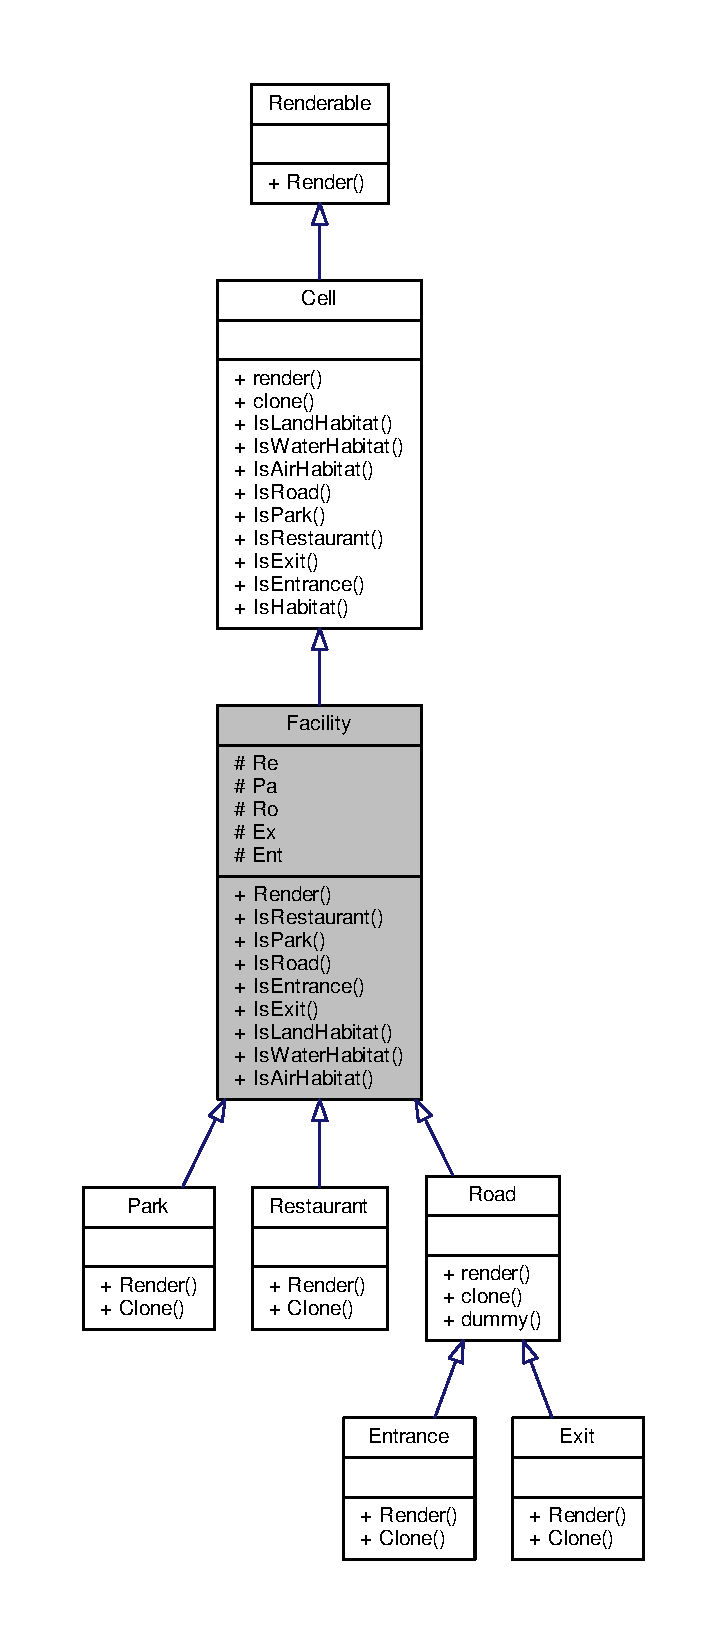
\includegraphics[height=550pt]{classFacility__inherit__graph}
\end{center}
\end{figure}


Collaboration diagram for Facility\+:
\nopagebreak
\begin{figure}[H]
\begin{center}
\leavevmode
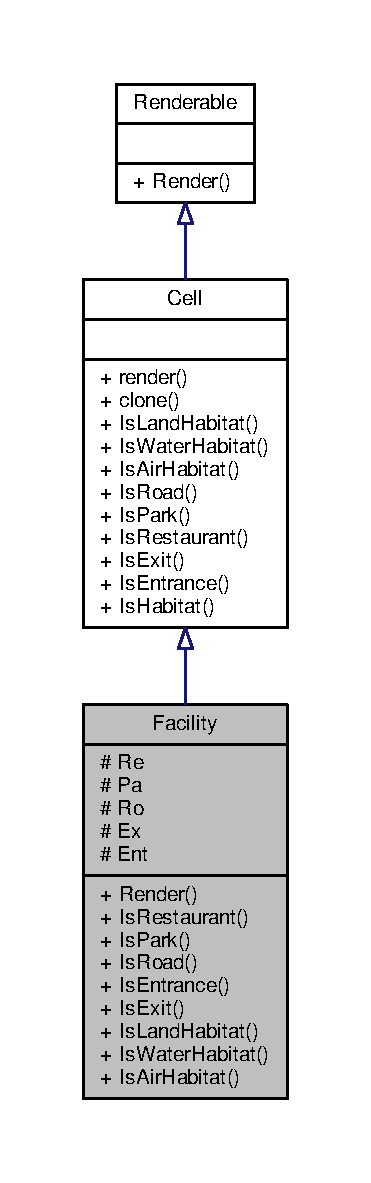
\includegraphics[height=550pt]{classFacility__coll__graph}
\end{center}
\end{figure}
\subsection*{Public Member Functions}
\begin{DoxyCompactItemize}
\item 
virtual char \hyperlink{classFacility_a177b3f9cd142fe4521c1d15b00d3675c}{Render} ()=0
\begin{DoxyCompactList}\small\item\em render \end{DoxyCompactList}\item 
virtual bool \hyperlink{classFacility_a2fb6a0e98e709b46b21e35cb8aeeeda7}{Is\+Restaurant} ()
\begin{DoxyCompactList}\small\item\em Memeriksa kode objek \hyperlink{classFacility}{Facility}. \end{DoxyCompactList}\item 
virtual bool \hyperlink{classFacility_acd5c991c33b331d67bb559f962d3bbc0}{Is\+Park} ()
\begin{DoxyCompactList}\small\item\em Memeriksa kode objek \hyperlink{classFacility}{Facility}. \end{DoxyCompactList}\item 
virtual bool \hyperlink{classFacility_ae2975cf479c3907e13fc200464b7443b}{Is\+Road} ()
\begin{DoxyCompactList}\small\item\em Memeriksa kode objek \hyperlink{classFacility}{Facility}. \end{DoxyCompactList}\item 
virtual bool \hyperlink{classFacility_a256cb0f3621b6545ec212d56672d5b3e}{Is\+Entrance} ()
\begin{DoxyCompactList}\small\item\em Memeriksa kode objek \hyperlink{classFacility}{Facility}. \end{DoxyCompactList}\item 
virtual bool \hyperlink{classFacility_aa6ed2cd4c8b1dc21a478c26707d16ef5}{Is\+Exit} ()
\begin{DoxyCompactList}\small\item\em Memeriksa kode objek \hyperlink{classFacility}{Facility}. \end{DoxyCompactList}\item 
virtual bool \hyperlink{classFacility_a1a8bbfab30dce85b0c581715cb4af1dd}{Is\+Land\+Habitat} ()
\begin{DoxyCompactList}\small\item\em Memeriksa kode objek \hyperlink{classFacility}{Facility}. \end{DoxyCompactList}\item 
virtual bool \hyperlink{classFacility_acaa21936227ef88450ab6834b5711a5c}{Is\+Water\+Habitat} ()
\begin{DoxyCompactList}\small\item\em Memeriksa kode objek \hyperlink{classFacility}{Facility}. \end{DoxyCompactList}\item 
virtual bool \hyperlink{classFacility_a6092a86c14a7c2003e2b020aa28fc06f}{Is\+Air\+Habitat} ()
\begin{DoxyCompactList}\small\item\em Memeriksa kode objek \hyperlink{classFacility}{Facility}. \end{DoxyCompactList}\end{DoxyCompactItemize}
\subsection*{Static Protected Attributes}
\begin{DoxyCompactItemize}
\item 
static const char \hyperlink{classFacility_a0c187566e945c796ffb5679d6c34287b}{Re} = \textquotesingle{}S\textquotesingle{}
\item 
static const char \hyperlink{classFacility_a5588f173a18205498f4c3bfd3c04d28c}{Pa} = \textquotesingle{}\#\textquotesingle{}
\item 
static const char \hyperlink{classFacility_ac6279190b255cdb87040af59e849543a}{Ro} = \textquotesingle{}+\textquotesingle{}
\item 
static const char \hyperlink{classFacility_ad30246918df96bd5a4e63063a1a1ae2e}{Ex} = \textquotesingle{}X\textquotesingle{}
\item 
static const char \hyperlink{classFacility_a2946221d924add37fc2a4aab5912dc60}{Ent} = \textquotesingle{}Z\textquotesingle{}
\end{DoxyCompactItemize}


\subsection{Detailed Description}
Kelas abstrak \hyperlink{classFacility}{Facility} merupakan simulasi dari fasilitas yang terdapat dalam kebun binatang 

\subsection{Member Function Documentation}
\index{Facility@{Facility}!Is\+Air\+Habitat@{Is\+Air\+Habitat}}
\index{Is\+Air\+Habitat@{Is\+Air\+Habitat}!Facility@{Facility}}
\subsubsection[{\texorpdfstring{Is\+Air\+Habitat()}{IsAirHabitat()}}]{\setlength{\rightskip}{0pt plus 5cm}virtual bool Facility\+::\+Is\+Air\+Habitat (
\begin{DoxyParamCaption}
{}
\end{DoxyParamCaption}
)\hspace{0.3cm}{\ttfamily [inline]}, {\ttfamily [virtual]}}\hypertarget{classFacility_a6092a86c14a7c2003e2b020aa28fc06f}{}\label{classFacility_a6092a86c14a7c2003e2b020aa28fc06f}


Memeriksa kode objek \hyperlink{classFacility}{Facility}. 

\begin{DoxyReturn}{Returns}
Mengembalikan nilai false. 
\end{DoxyReturn}


Implements \hyperlink{classCell_a24f8abceee9ce115d47b588992407a4d}{Cell}.

\index{Facility@{Facility}!Is\+Entrance@{Is\+Entrance}}
\index{Is\+Entrance@{Is\+Entrance}!Facility@{Facility}}
\subsubsection[{\texorpdfstring{Is\+Entrance()}{IsEntrance()}}]{\setlength{\rightskip}{0pt plus 5cm}virtual bool Facility\+::\+Is\+Entrance (
\begin{DoxyParamCaption}
{}
\end{DoxyParamCaption}
)\hspace{0.3cm}{\ttfamily [inline]}, {\ttfamily [virtual]}}\hypertarget{classFacility_a256cb0f3621b6545ec212d56672d5b3e}{}\label{classFacility_a256cb0f3621b6545ec212d56672d5b3e}


Memeriksa kode objek \hyperlink{classFacility}{Facility}. 

\begin{DoxyReturn}{Returns}
Mengembalikan true jika \hyperlink{classFacility}{Facility} merupakan \hyperlink{classEntrance}{Entrance}. 
\end{DoxyReturn}


Implements \hyperlink{classCell_ab10ef0ffe5c971c59d0e6167131dd521}{Cell}.

\index{Facility@{Facility}!Is\+Exit@{Is\+Exit}}
\index{Is\+Exit@{Is\+Exit}!Facility@{Facility}}
\subsubsection[{\texorpdfstring{Is\+Exit()}{IsExit()}}]{\setlength{\rightskip}{0pt plus 5cm}virtual bool Facility\+::\+Is\+Exit (
\begin{DoxyParamCaption}
{}
\end{DoxyParamCaption}
)\hspace{0.3cm}{\ttfamily [inline]}, {\ttfamily [virtual]}}\hypertarget{classFacility_aa6ed2cd4c8b1dc21a478c26707d16ef5}{}\label{classFacility_aa6ed2cd4c8b1dc21a478c26707d16ef5}


Memeriksa kode objek \hyperlink{classFacility}{Facility}. 

\begin{DoxyReturn}{Returns}
Mengembalikan true jika \hyperlink{classFacility}{Facility} merupakan \hyperlink{classExit}{Exit}. 
\end{DoxyReturn}


Implements \hyperlink{classCell_adfef5e446c31ace0e9fef1235e4f8fef}{Cell}.

\index{Facility@{Facility}!Is\+Land\+Habitat@{Is\+Land\+Habitat}}
\index{Is\+Land\+Habitat@{Is\+Land\+Habitat}!Facility@{Facility}}
\subsubsection[{\texorpdfstring{Is\+Land\+Habitat()}{IsLandHabitat()}}]{\setlength{\rightskip}{0pt plus 5cm}virtual bool Facility\+::\+Is\+Land\+Habitat (
\begin{DoxyParamCaption}
{}
\end{DoxyParamCaption}
)\hspace{0.3cm}{\ttfamily [inline]}, {\ttfamily [virtual]}}\hypertarget{classFacility_a1a8bbfab30dce85b0c581715cb4af1dd}{}\label{classFacility_a1a8bbfab30dce85b0c581715cb4af1dd}


Memeriksa kode objek \hyperlink{classFacility}{Facility}. 

\begin{DoxyReturn}{Returns}
Mengembalikan nilai false. 
\end{DoxyReturn}


Implements \hyperlink{classCell_a6cc005c27ee600d76a91459b7733b90e}{Cell}.

\index{Facility@{Facility}!Is\+Park@{Is\+Park}}
\index{Is\+Park@{Is\+Park}!Facility@{Facility}}
\subsubsection[{\texorpdfstring{Is\+Park()}{IsPark()}}]{\setlength{\rightskip}{0pt plus 5cm}virtual bool Facility\+::\+Is\+Park (
\begin{DoxyParamCaption}
{}
\end{DoxyParamCaption}
)\hspace{0.3cm}{\ttfamily [inline]}, {\ttfamily [virtual]}}\hypertarget{classFacility_acd5c991c33b331d67bb559f962d3bbc0}{}\label{classFacility_acd5c991c33b331d67bb559f962d3bbc0}


Memeriksa kode objek \hyperlink{classFacility}{Facility}. 

\begin{DoxyReturn}{Returns}
Mengembalikan true jika \hyperlink{classFacility}{Facility} merupakan \hyperlink{classPark}{Park}. 
\end{DoxyReturn}


Implements \hyperlink{classCell_ad87cbdb9c06b19c7c6571053c3888a51}{Cell}.

\index{Facility@{Facility}!Is\+Restaurant@{Is\+Restaurant}}
\index{Is\+Restaurant@{Is\+Restaurant}!Facility@{Facility}}
\subsubsection[{\texorpdfstring{Is\+Restaurant()}{IsRestaurant()}}]{\setlength{\rightskip}{0pt plus 5cm}virtual bool Facility\+::\+Is\+Restaurant (
\begin{DoxyParamCaption}
{}
\end{DoxyParamCaption}
)\hspace{0.3cm}{\ttfamily [inline]}, {\ttfamily [virtual]}}\hypertarget{classFacility_a2fb6a0e98e709b46b21e35cb8aeeeda7}{}\label{classFacility_a2fb6a0e98e709b46b21e35cb8aeeeda7}


Memeriksa kode objek \hyperlink{classFacility}{Facility}. 

\begin{DoxyReturn}{Returns}
Mengembalikan true jika \hyperlink{classFacility}{Facility} merupakan \hyperlink{classRestaurant}{Restaurant}. 
\end{DoxyReturn}


Implements \hyperlink{classCell_a804041eef60df6b659032dc5a1fe3854}{Cell}.

\index{Facility@{Facility}!Is\+Road@{Is\+Road}}
\index{Is\+Road@{Is\+Road}!Facility@{Facility}}
\subsubsection[{\texorpdfstring{Is\+Road()}{IsRoad()}}]{\setlength{\rightskip}{0pt plus 5cm}virtual bool Facility\+::\+Is\+Road (
\begin{DoxyParamCaption}
{}
\end{DoxyParamCaption}
)\hspace{0.3cm}{\ttfamily [inline]}, {\ttfamily [virtual]}}\hypertarget{classFacility_ae2975cf479c3907e13fc200464b7443b}{}\label{classFacility_ae2975cf479c3907e13fc200464b7443b}


Memeriksa kode objek \hyperlink{classFacility}{Facility}. 

\begin{DoxyReturn}{Returns}
Mengembalikan true jika \hyperlink{classFacility}{Facility} merupakan \hyperlink{classRoad}{Road}, \hyperlink{classEntrance}{Entrance}, atau \hyperlink{classExit}{Exit}. 
\end{DoxyReturn}


Implements \hyperlink{classCell_a6afd033fa34492761e1de9fd1f7c8a95}{Cell}.

\index{Facility@{Facility}!Is\+Water\+Habitat@{Is\+Water\+Habitat}}
\index{Is\+Water\+Habitat@{Is\+Water\+Habitat}!Facility@{Facility}}
\subsubsection[{\texorpdfstring{Is\+Water\+Habitat()}{IsWaterHabitat()}}]{\setlength{\rightskip}{0pt plus 5cm}virtual bool Facility\+::\+Is\+Water\+Habitat (
\begin{DoxyParamCaption}
{}
\end{DoxyParamCaption}
)\hspace{0.3cm}{\ttfamily [inline]}, {\ttfamily [virtual]}}\hypertarget{classFacility_acaa21936227ef88450ab6834b5711a5c}{}\label{classFacility_acaa21936227ef88450ab6834b5711a5c}


Memeriksa kode objek \hyperlink{classFacility}{Facility}. 

\begin{DoxyReturn}{Returns}
Mengembalikan nilai false. 
\end{DoxyReturn}


Implements \hyperlink{classCell_af620aac2cb7ce59657ca158255462fef}{Cell}.

\index{Facility@{Facility}!Render@{Render}}
\index{Render@{Render}!Facility@{Facility}}
\subsubsection[{\texorpdfstring{Render()=0}{Render()=0}}]{\setlength{\rightskip}{0pt plus 5cm}virtual char Facility\+::\+Render (
\begin{DoxyParamCaption}
{}
\end{DoxyParamCaption}
)\hspace{0.3cm}{\ttfamily [pure virtual]}}\hypertarget{classFacility_a177b3f9cd142fe4521c1d15b00d3675c}{}\label{classFacility_a177b3f9cd142fe4521c1d15b00d3675c}


render 

\begin{DoxyReturn}{Returns}
Mengembalikan char yang merupakan representasi kode objek fasilitas. 
\end{DoxyReturn}


Implements \hyperlink{classRenderable_a923171f6811c24ae6808c1a8639a5c81}{Renderable}.



Implemented in \hyperlink{classEntrance_a7226e0cd3d04f8370ede2573bc2852f3}{Entrance}, \hyperlink{classExit_a9239e8b13c101d1aee8fde738e8a5fdc}{Exit}, \hyperlink{classPark_a98b2a346d5ec6703b2e988588950947e}{Park}, and \hyperlink{classRestaurant_a8a44dac5fd1d460aed3a5631e9eb732a}{Restaurant}.



\subsection{Member Data Documentation}
\index{Facility@{Facility}!Ent@{Ent}}
\index{Ent@{Ent}!Facility@{Facility}}
\subsubsection[{\texorpdfstring{Ent}{Ent}}]{\setlength{\rightskip}{0pt plus 5cm}const char Facility\+::\+Ent = \textquotesingle{}Z\textquotesingle{}\hspace{0.3cm}{\ttfamily [static]}, {\ttfamily [protected]}}\hypertarget{classFacility_a2946221d924add37fc2a4aab5912dc60}{}\label{classFacility_a2946221d924add37fc2a4aab5912dc60}
\index{Facility@{Facility}!Ex@{Ex}}
\index{Ex@{Ex}!Facility@{Facility}}
\subsubsection[{\texorpdfstring{Ex}{Ex}}]{\setlength{\rightskip}{0pt plus 5cm}const char Facility\+::\+Ex = \textquotesingle{}X\textquotesingle{}\hspace{0.3cm}{\ttfamily [static]}, {\ttfamily [protected]}}\hypertarget{classFacility_ad30246918df96bd5a4e63063a1a1ae2e}{}\label{classFacility_ad30246918df96bd5a4e63063a1a1ae2e}
\index{Facility@{Facility}!Pa@{Pa}}
\index{Pa@{Pa}!Facility@{Facility}}
\subsubsection[{\texorpdfstring{Pa}{Pa}}]{\setlength{\rightskip}{0pt plus 5cm}const char Facility\+::\+Pa = \textquotesingle{}\#\textquotesingle{}\hspace{0.3cm}{\ttfamily [static]}, {\ttfamily [protected]}}\hypertarget{classFacility_a5588f173a18205498f4c3bfd3c04d28c}{}\label{classFacility_a5588f173a18205498f4c3bfd3c04d28c}
\index{Facility@{Facility}!Re@{Re}}
\index{Re@{Re}!Facility@{Facility}}
\subsubsection[{\texorpdfstring{Re}{Re}}]{\setlength{\rightskip}{0pt plus 5cm}const char Facility\+::\+Re = \textquotesingle{}S\textquotesingle{}\hspace{0.3cm}{\ttfamily [static]}, {\ttfamily [protected]}}\hypertarget{classFacility_a0c187566e945c796ffb5679d6c34287b}{}\label{classFacility_a0c187566e945c796ffb5679d6c34287b}
\index{Facility@{Facility}!Ro@{Ro}}
\index{Ro@{Ro}!Facility@{Facility}}
\subsubsection[{\texorpdfstring{Ro}{Ro}}]{\setlength{\rightskip}{0pt plus 5cm}const char Facility\+::\+Ro = \textquotesingle{}+\textquotesingle{}\hspace{0.3cm}{\ttfamily [static]}, {\ttfamily [protected]}}\hypertarget{classFacility_ac6279190b255cdb87040af59e849543a}{}\label{classFacility_ac6279190b255cdb87040af59e849543a}


The documentation for this class was generated from the following file\+:\begin{DoxyCompactItemize}
\item 
\hyperlink{facility_8h}{facility.\+h}\end{DoxyCompactItemize}

\hypertarget{classFlyingAnimal}{}\section{Flying\+Animal Class Reference}
\label{classFlyingAnimal}\index{Flying\+Animal@{Flying\+Animal}}


{\ttfamily \#include $<$flying\+\_\+animal.\+h$>$}



Inheritance diagram for Flying\+Animal\+:
\nopagebreak
\begin{figure}[H]
\begin{center}
\leavevmode
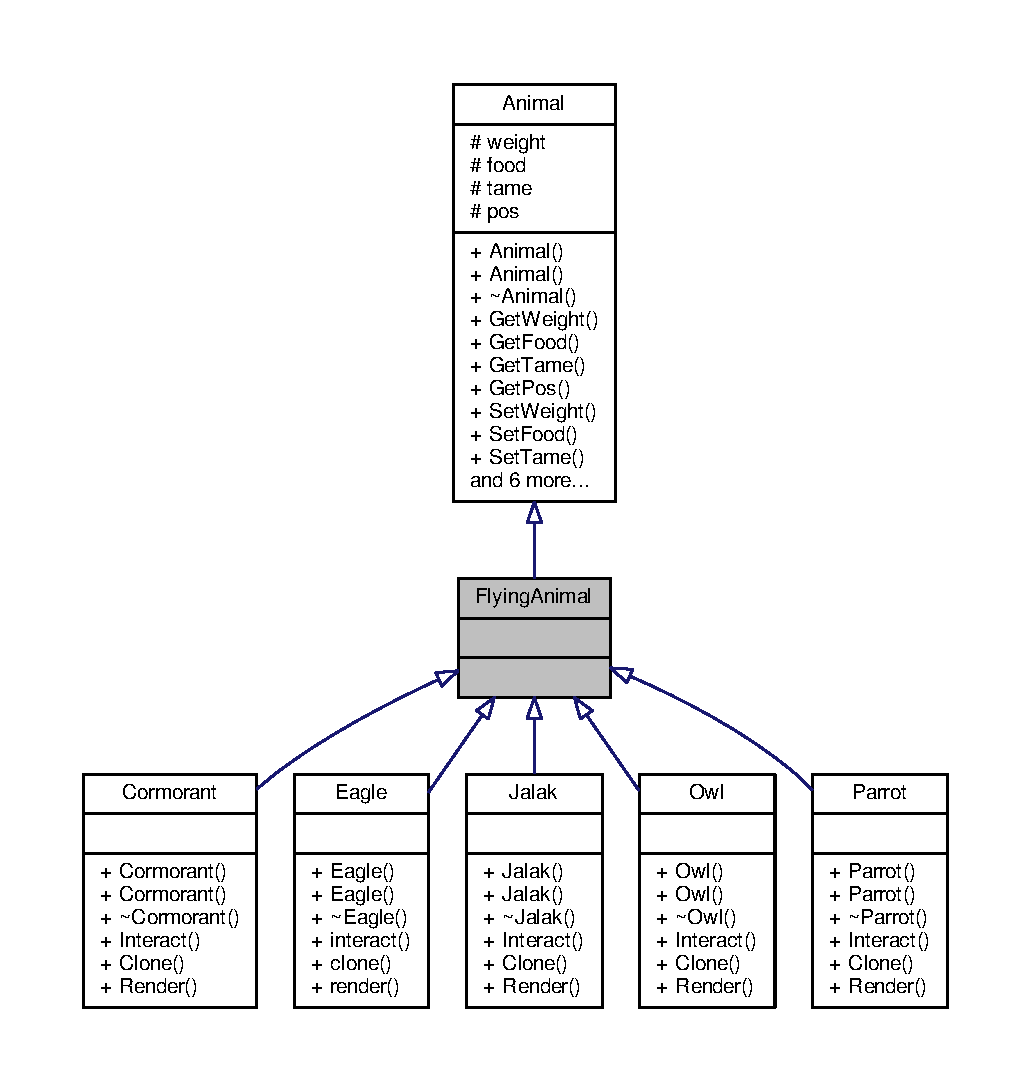
\includegraphics[width=350pt]{classFlyingAnimal__inherit__graph}
\end{center}
\end{figure}


Collaboration diagram for Flying\+Animal\+:
\nopagebreak
\begin{figure}[H]
\begin{center}
\leavevmode
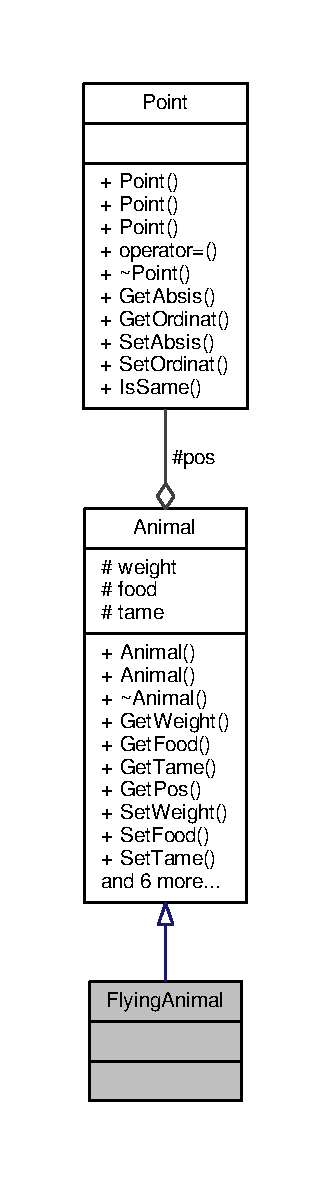
\includegraphics[height=550pt]{classFlyingAnimal__coll__graph}
\end{center}
\end{figure}
\subsection*{Additional Inherited Members}


\subsection{Detailed Description}
Kelas abstrak \hyperlink{classFlyingAnimal}{Flying\+Animal} merupakan kelas bagi animal dengan habitat di udara 

The documentation for this class was generated from the following file\+:\begin{DoxyCompactItemize}
\item 
\hyperlink{flying__animal_8h}{flying\+\_\+animal.\+h}\end{DoxyCompactItemize}

\hypertarget{classGiraffe}{}\section{Giraffe Class Reference}
\label{classGiraffe}\index{Giraffe@{Giraffe}}


{\ttfamily \#include $<$giraffe.\+h$>$}



Inheritance diagram for Giraffe\+:
\nopagebreak
\begin{figure}[H]
\begin{center}
\leavevmode
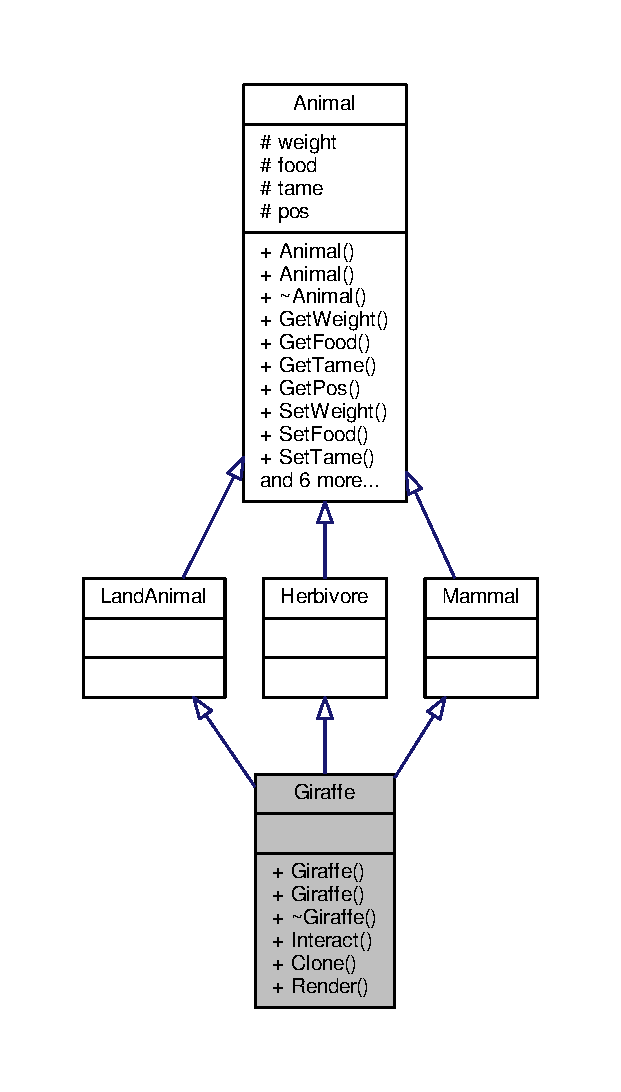
\includegraphics[width=220pt]{classGiraffe__inherit__graph}
\end{center}
\end{figure}


Collaboration diagram for Giraffe\+:
\nopagebreak
\begin{figure}[H]
\begin{center}
\leavevmode
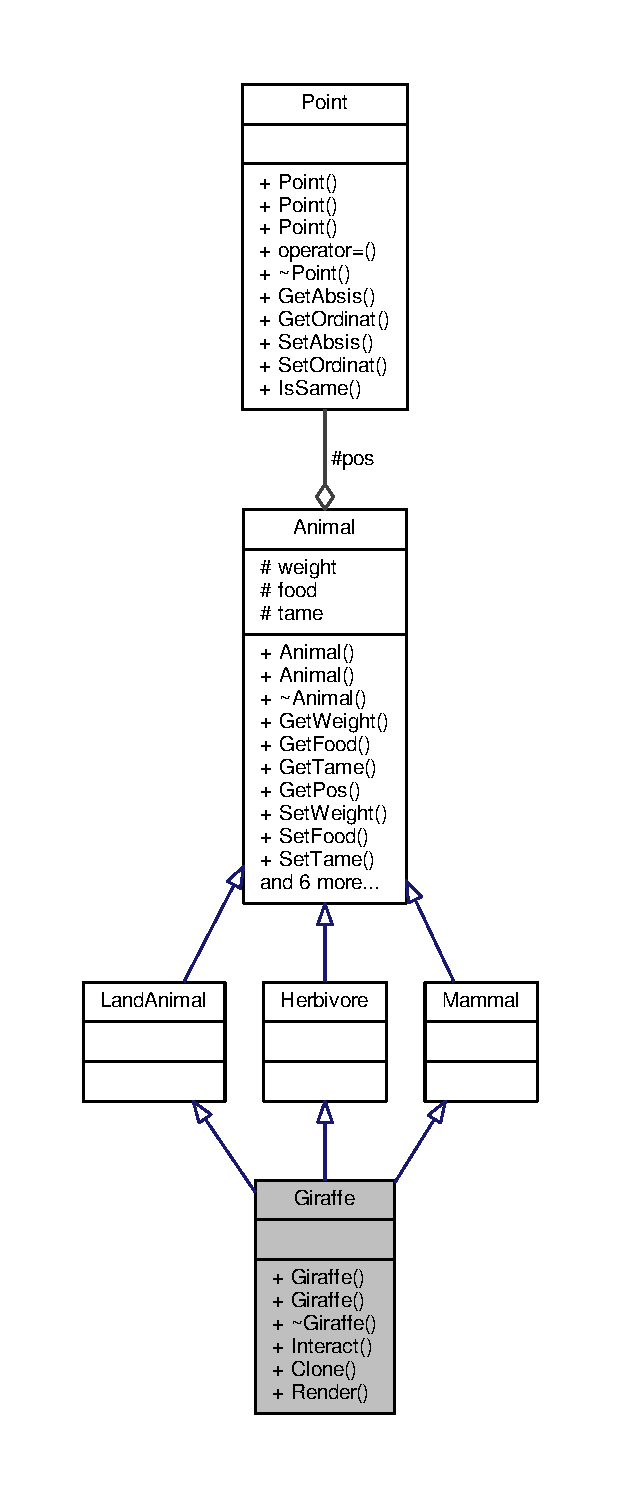
\includegraphics[height=550pt]{classGiraffe__coll__graph}
\end{center}
\end{figure}
\subsection*{Public Member Functions}
\begin{DoxyCompactItemize}
\item 
\hyperlink{classGiraffe_a4a396bd3e634243c1740916b71197168}{Giraffe} ()
\begin{DoxyCompactList}\small\item\em Constructor. Menciptakan objek \hyperlink{classGiraffe}{Giraffe}. \end{DoxyCompactList}\item 
virtual \hyperlink{classGiraffe_a1d099c4a2c87fbac26e5bcb33084dcb4}{$\sim$\+Giraffe} ()
\begin{DoxyCompactList}\small\item\em Destructor. \end{DoxyCompactList}\item 
string \hyperlink{classGiraffe_ad73e5ee5fc62f709c52a1cab68f2a1f3}{Interact} ()
\begin{DoxyCompactList}\small\item\em Interaksi yang dilakukan \hyperlink{classGiraffe}{Giraffe}. \end{DoxyCompactList}\item 
virtual \hyperlink{classGiraffe}{Giraffe} $\ast$ \hyperlink{classGiraffe_aa29f8f77477a64fc72f814b7f225c94f}{Clone} () const 
\begin{DoxyCompactList}\small\item\em Melakukan cloning untuk menciptakan objek \hyperlink{classGiraffe}{Giraffe} baru. \end{DoxyCompactList}\item 
char \hyperlink{classGiraffe_a64dccf030fdb54de9fd37f8381c64271}{Render} ()
\begin{DoxyCompactList}\small\item\em Render dari \hyperlink{classGiraffe}{Giraffe}. \end{DoxyCompactList}\end{DoxyCompactItemize}
\subsection*{Additional Inherited Members}


\subsection{Detailed Description}
Kelas \hyperlink{classGiraffe}{Giraffe} merupakan kelas untuk real object \hyperlink{classGiraffe}{Giraffe} 

\subsection{Constructor \& Destructor Documentation}
\index{Giraffe@{Giraffe}!Giraffe@{Giraffe}}
\index{Giraffe@{Giraffe}!Giraffe@{Giraffe}}
\subsubsection[{\texorpdfstring{Giraffe()}{Giraffe()}}]{\setlength{\rightskip}{0pt plus 5cm}Giraffe\+::\+Giraffe (
\begin{DoxyParamCaption}
{}
\end{DoxyParamCaption}
)\hspace{0.3cm}{\ttfamily [inline]}}\hypertarget{classGiraffe_a4a396bd3e634243c1740916b71197168}{}\label{classGiraffe_a4a396bd3e634243c1740916b71197168}


Constructor. Menciptakan objek \hyperlink{classGiraffe}{Giraffe}. 

\index{Giraffe@{Giraffe}!````~Giraffe@{$\sim$\+Giraffe}}
\index{````~Giraffe@{$\sim$\+Giraffe}!Giraffe@{Giraffe}}
\subsubsection[{\texorpdfstring{$\sim$\+Giraffe()}{~Giraffe()}}]{\setlength{\rightskip}{0pt plus 5cm}virtual Giraffe\+::$\sim$\+Giraffe (
\begin{DoxyParamCaption}
{}
\end{DoxyParamCaption}
)\hspace{0.3cm}{\ttfamily [inline]}, {\ttfamily [virtual]}}\hypertarget{classGiraffe_a1d099c4a2c87fbac26e5bcb33084dcb4}{}\label{classGiraffe_a1d099c4a2c87fbac26e5bcb33084dcb4}


Destructor. 



\subsection{Member Function Documentation}
\index{Giraffe@{Giraffe}!Clone@{Clone}}
\index{Clone@{Clone}!Giraffe@{Giraffe}}
\subsubsection[{\texorpdfstring{Clone() const }{Clone() const }}]{\setlength{\rightskip}{0pt plus 5cm}virtual {\bf Giraffe}$\ast$ Giraffe\+::\+Clone (
\begin{DoxyParamCaption}
{}
\end{DoxyParamCaption}
) const\hspace{0.3cm}{\ttfamily [inline]}, {\ttfamily [virtual]}}\hypertarget{classGiraffe_aa29f8f77477a64fc72f814b7f225c94f}{}\label{classGiraffe_aa29f8f77477a64fc72f814b7f225c94f}


Melakukan cloning untuk menciptakan objek \hyperlink{classGiraffe}{Giraffe} baru. 

\begin{DoxyReturn}{Returns}
Mengembalikan pointer to \hyperlink{classGiraffe}{Giraffe} objek tersebut. 
\end{DoxyReturn}


Implements \hyperlink{classAnimal_a3fc95e2a588b653b9b315e6c7a29c89f}{Animal}.

\index{Giraffe@{Giraffe}!Interact@{Interact}}
\index{Interact@{Interact}!Giraffe@{Giraffe}}
\subsubsection[{\texorpdfstring{Interact()}{Interact()}}]{\setlength{\rightskip}{0pt plus 5cm}string Giraffe\+::\+Interact (
\begin{DoxyParamCaption}
{}
\end{DoxyParamCaption}
)\hspace{0.3cm}{\ttfamily [inline]}, {\ttfamily [virtual]}}\hypertarget{classGiraffe_ad73e5ee5fc62f709c52a1cab68f2a1f3}{}\label{classGiraffe_ad73e5ee5fc62f709c52a1cab68f2a1f3}


Interaksi yang dilakukan \hyperlink{classGiraffe}{Giraffe}. 

\begin{DoxyReturn}{Returns}
Mengembalikan string yang merepresentasikan suara \hyperlink{classGiraffe}{Giraffe}. 
\end{DoxyReturn}


Implements \hyperlink{classAnimal_ad5a55fb0355a9425fee6611003d9892c}{Animal}.

\index{Giraffe@{Giraffe}!Render@{Render}}
\index{Render@{Render}!Giraffe@{Giraffe}}
\subsubsection[{\texorpdfstring{Render()}{Render()}}]{\setlength{\rightskip}{0pt plus 5cm}char Giraffe\+::\+Render (
\begin{DoxyParamCaption}
{}
\end{DoxyParamCaption}
)\hspace{0.3cm}{\ttfamily [inline]}, {\ttfamily [virtual]}}\hypertarget{classGiraffe_a64dccf030fdb54de9fd37f8381c64271}{}\label{classGiraffe_a64dccf030fdb54de9fd37f8381c64271}


Render dari \hyperlink{classGiraffe}{Giraffe}. 

\begin{DoxyReturn}{Returns}
Mengembalikan char yang merupakan representasi kode \hyperlink{classGiraffe}{Giraffe}. 
\end{DoxyReturn}


Implements \hyperlink{classAnimal_a43a47c0f41d211128e04abc6add53def}{Animal}.



The documentation for this class was generated from the following file\+:\begin{DoxyCompactItemize}
\item 
giraffe/\hyperlink{giraffe_8h}{giraffe.\+h}\end{DoxyCompactItemize}

\hypertarget{classGoat}{}\section{Goat Class Reference}
\label{classGoat}\index{Goat@{Goat}}


{\ttfamily \#include $<$goat.\+h$>$}



Inheritance diagram for Goat\+:
\nopagebreak
\begin{figure}[H]
\begin{center}
\leavevmode
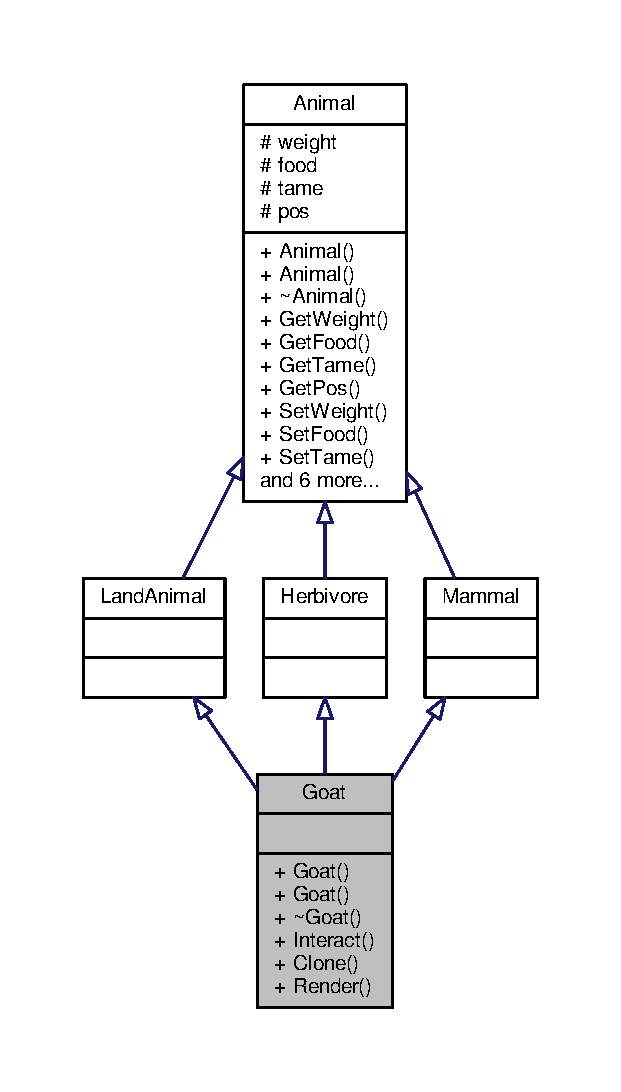
\includegraphics[width=220pt]{classGoat__inherit__graph}
\end{center}
\end{figure}


Collaboration diagram for Goat\+:
\nopagebreak
\begin{figure}[H]
\begin{center}
\leavevmode
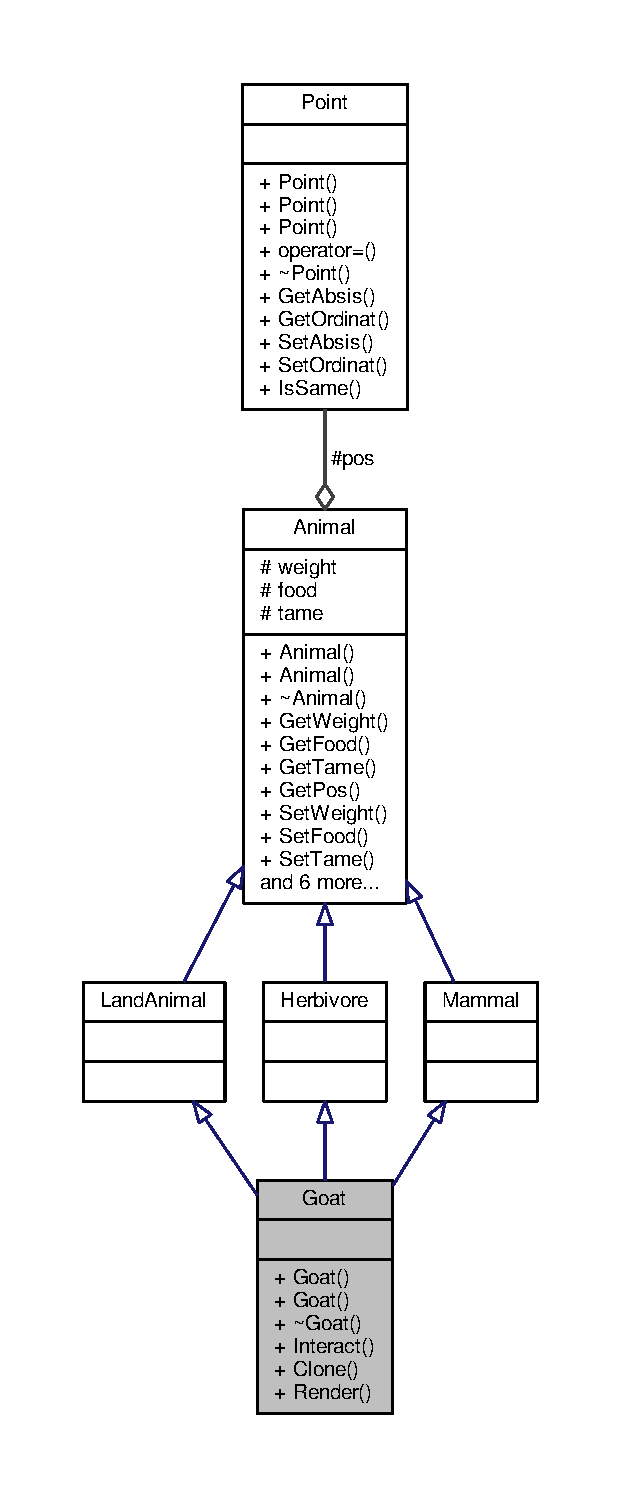
\includegraphics[height=550pt]{classGoat__coll__graph}
\end{center}
\end{figure}
\subsection*{Public Member Functions}
\begin{DoxyCompactItemize}
\item 
\hyperlink{classGoat_acf506b76c8503c9749df191a92dc99f9}{Goat} ()
\begin{DoxyCompactList}\small\item\em Constructor. Menciptakan objek \hyperlink{classGoat}{Goat}. \end{DoxyCompactList}\item 
virtual \hyperlink{classGoat_a47af45317eec8718356b20a10e31af27}{$\sim$\+Goat} ()
\begin{DoxyCompactList}\small\item\em Destructor. \end{DoxyCompactList}\item 
string \hyperlink{classGoat_a5f480d88c50724cee8c7a9d18f486144}{Interact} ()
\begin{DoxyCompactList}\small\item\em Interaksi yang dilakukan \hyperlink{classGoat}{Goat}. \end{DoxyCompactList}\item 
virtual \hyperlink{classGoat}{Goat} $\ast$ \hyperlink{classGoat_a1532200ef20734bb42d0a1306b14d8ad}{Clone} () const 
\begin{DoxyCompactList}\small\item\em Melakukan cloning untuk menciptakan objek \hyperlink{classGoat}{Goat} baru. \end{DoxyCompactList}\item 
char \hyperlink{classGoat_aedea4680fe17571c2f51d35b90397f6e}{Render} ()
\begin{DoxyCompactList}\small\item\em Render dari \hyperlink{classGoat}{Goat}. \end{DoxyCompactList}\end{DoxyCompactItemize}
\subsection*{Additional Inherited Members}


\subsection{Detailed Description}
Kelas \hyperlink{classGoat}{Goat} merupakan kelas untuk real object \hyperlink{classGoat}{Goat} 

\subsection{Constructor \& Destructor Documentation}
\index{Goat@{Goat}!Goat@{Goat}}
\index{Goat@{Goat}!Goat@{Goat}}
\subsubsection[{\texorpdfstring{Goat()}{Goat()}}]{\setlength{\rightskip}{0pt plus 5cm}Goat\+::\+Goat (
\begin{DoxyParamCaption}
{}
\end{DoxyParamCaption}
)\hspace{0.3cm}{\ttfamily [inline]}}\hypertarget{classGoat_acf506b76c8503c9749df191a92dc99f9}{}\label{classGoat_acf506b76c8503c9749df191a92dc99f9}


Constructor. Menciptakan objek \hyperlink{classGoat}{Goat}. 

\index{Goat@{Goat}!````~Goat@{$\sim$\+Goat}}
\index{````~Goat@{$\sim$\+Goat}!Goat@{Goat}}
\subsubsection[{\texorpdfstring{$\sim$\+Goat()}{~Goat()}}]{\setlength{\rightskip}{0pt plus 5cm}virtual Goat\+::$\sim$\+Goat (
\begin{DoxyParamCaption}
{}
\end{DoxyParamCaption}
)\hspace{0.3cm}{\ttfamily [inline]}, {\ttfamily [virtual]}}\hypertarget{classGoat_a47af45317eec8718356b20a10e31af27}{}\label{classGoat_a47af45317eec8718356b20a10e31af27}


Destructor. 



\subsection{Member Function Documentation}
\index{Goat@{Goat}!Clone@{Clone}}
\index{Clone@{Clone}!Goat@{Goat}}
\subsubsection[{\texorpdfstring{Clone() const }{Clone() const }}]{\setlength{\rightskip}{0pt plus 5cm}virtual {\bf Goat}$\ast$ Goat\+::\+Clone (
\begin{DoxyParamCaption}
{}
\end{DoxyParamCaption}
) const\hspace{0.3cm}{\ttfamily [inline]}, {\ttfamily [virtual]}}\hypertarget{classGoat_a1532200ef20734bb42d0a1306b14d8ad}{}\label{classGoat_a1532200ef20734bb42d0a1306b14d8ad}


Melakukan cloning untuk menciptakan objek \hyperlink{classGoat}{Goat} baru. 

\begin{DoxyReturn}{Returns}
Mengembalikan pointer to \hyperlink{classGoat}{Goat} objek tersebut. 
\end{DoxyReturn}


Implements \hyperlink{classAnimal_a3fc95e2a588b653b9b315e6c7a29c89f}{Animal}.

\index{Goat@{Goat}!Interact@{Interact}}
\index{Interact@{Interact}!Goat@{Goat}}
\subsubsection[{\texorpdfstring{Interact()}{Interact()}}]{\setlength{\rightskip}{0pt plus 5cm}string Goat\+::\+Interact (
\begin{DoxyParamCaption}
{}
\end{DoxyParamCaption}
)\hspace{0.3cm}{\ttfamily [inline]}, {\ttfamily [virtual]}}\hypertarget{classGoat_a5f480d88c50724cee8c7a9d18f486144}{}\label{classGoat_a5f480d88c50724cee8c7a9d18f486144}


Interaksi yang dilakukan \hyperlink{classGoat}{Goat}. 

\begin{DoxyReturn}{Returns}
Mengembalikan string yang merepresentasikan suara \hyperlink{classGoat}{Goat}. 
\end{DoxyReturn}


Implements \hyperlink{classAnimal_ad5a55fb0355a9425fee6611003d9892c}{Animal}.

\index{Goat@{Goat}!Render@{Render}}
\index{Render@{Render}!Goat@{Goat}}
\subsubsection[{\texorpdfstring{Render()}{Render()}}]{\setlength{\rightskip}{0pt plus 5cm}char Goat\+::\+Render (
\begin{DoxyParamCaption}
{}
\end{DoxyParamCaption}
)\hspace{0.3cm}{\ttfamily [inline]}, {\ttfamily [virtual]}}\hypertarget{classGoat_aedea4680fe17571c2f51d35b90397f6e}{}\label{classGoat_aedea4680fe17571c2f51d35b90397f6e}


Render dari \hyperlink{classGoat}{Goat}. 

\begin{DoxyReturn}{Returns}
Mengembalikan char yang merupakan representasi kode \hyperlink{classGoat}{Goat}. 
\end{DoxyReturn}


Implements \hyperlink{classAnimal_a43a47c0f41d211128e04abc6add53def}{Animal}.



The documentation for this class was generated from the following file\+:\begin{DoxyCompactItemize}
\item 
goat/\hyperlink{goat_8h}{goat.\+h}\end{DoxyCompactItemize}

\hypertarget{classHabitat}{}\section{Habitat Class Reference}
\label{classHabitat}\index{Habitat@{Habitat}}


{\ttfamily \#include $<$habitat.\+h$>$}



Inheritance diagram for Habitat\+:
% FIG 0


Collaboration diagram for Habitat\+:
% FIG 1
\subsection*{Public Member Functions}
\begin{DoxyCompactItemize}
\item 
virtual char \hyperlink{classHabitat_ad1bf10205d38e8e308eb9acc3aa2872c}{Render} ()=0
\begin{DoxyCompactList}\small\item\em Render dari \hyperlink{classHabitat}{Habitat}. \end{DoxyCompactList}\item 
virtual bool \hyperlink{classHabitat_aaf69aab7e1ce1075188651d2cb388b6b}{Is\+Land\+Habitat} ()
\begin{DoxyCompactList}\small\item\em Menentukan apakah \hyperlink{classHabitat}{Habitat} merupakan \hyperlink{classLandHabitat}{Land\+Habitat}. \end{DoxyCompactList}\item 
virtual bool \hyperlink{classHabitat_acfdb3e3911d536c5564c91d60c368fc4}{Is\+Water\+Habitat} ()
\begin{DoxyCompactList}\small\item\em Menentukan apakah \hyperlink{classHabitat}{Habitat} merupakan \hyperlink{classWaterHabitat}{Water\+Habitat}. \end{DoxyCompactList}\item 
virtual bool \hyperlink{classHabitat_aef29f87fdc6be7ae4e44279d816e173b}{Is\+Air\+Habitat} ()
\begin{DoxyCompactList}\small\item\em Menentukan apakah \hyperlink{classHabitat}{Habitat} merupakan \hyperlink{classAirHabitat}{Air\+Habitat}. \end{DoxyCompactList}\item 
virtual bool \hyperlink{classHabitat_aedc03784a83bef591a2441d1c062cd57}{Is\+Entrance} ()
\begin{DoxyCompactList}\small\item\em Menentukan apakah \hyperlink{classHabitat}{Habitat} merupakan \hyperlink{classEntrance}{Entrance}. \end{DoxyCompactList}\item 
virtual bool \hyperlink{classHabitat_aece5f38292630cf5860001ae8fdd084d}{Is\+Exit} ()
\begin{DoxyCompactList}\small\item\em Menentukan apakah \hyperlink{classHabitat}{Habitat} merupakan \hyperlink{classExit}{Exit}. \end{DoxyCompactList}\item 
virtual bool \hyperlink{classHabitat_a0ab72de6d88706b4eb693ea2a2c7de53}{Is\+Restaurant} ()
\begin{DoxyCompactList}\small\item\em Menentukan apakah \hyperlink{classHabitat}{Habitat} merupakan \hyperlink{classRestaurant}{Restaurant}. \end{DoxyCompactList}\item 
virtual bool \hyperlink{classHabitat_aa4cd06885065d8b7e3c4477c626d2fe7}{Is\+Park} ()
\begin{DoxyCompactList}\small\item\em Menentukan apakah \hyperlink{classHabitat}{Habitat} merupakan \hyperlink{classPark}{Park}. \end{DoxyCompactList}\item 
virtual bool \hyperlink{classHabitat_aafd95775cc1e0876b40955c3e0126fe3}{Is\+Road} ()
\begin{DoxyCompactList}\small\item\em Menentukan apakah \hyperlink{classHabitat}{Habitat} merupakan \hyperlink{classRoad}{Road}. \end{DoxyCompactList}\end{DoxyCompactItemize}
\subsection*{Static Protected Attributes}
\begin{DoxyCompactItemize}
\item 
static const char \hyperlink{classHabitat_a87fbedb46cde325396e3ef39350e14d7}{LH} = \textquotesingle{}@\textquotesingle{}
\begin{DoxyCompactList}\small\item\em Representasi \hyperlink{classLandHabitat}{Land\+Habitat} ketika dicetak ke layar. \end{DoxyCompactList}\item 
static const char \hyperlink{classHabitat_af5c4388fa9d305995799c61cc6f5231d}{AH} = \textquotesingle{}$^\wedge$\textquotesingle{}
\begin{DoxyCompactList}\small\item\em Representasi \hyperlink{classAirHabitat}{Air\+Habitat} ketika dicetak ke layar. \end{DoxyCompactList}\item 
static const char \hyperlink{classHabitat_aeba269066b13b0f7b632526af4d547d3}{WH} = \textquotesingle{}$\sim$\textquotesingle{}
\begin{DoxyCompactList}\small\item\em Representasi \hyperlink{classWaterHabitat}{Water\+Habitat} ketika dicetak ke layar. \end{DoxyCompactList}\end{DoxyCompactItemize}


\subsection{Detailed Description}
Kelas abstrak \hyperlink{classHabitat}{Habitat} merupakan simulasi dari habitat 

\subsection{Member Function Documentation}
\index{Habitat@{Habitat}!Is\+Air\+Habitat@{Is\+Air\+Habitat}}
\index{Is\+Air\+Habitat@{Is\+Air\+Habitat}!Habitat@{Habitat}}
\subsubsection[{\texorpdfstring{Is\+Air\+Habitat()}{IsAirHabitat()}}]{\setlength{\rightskip}{0pt plus 5cm}virtual bool Habitat\+::\+Is\+Air\+Habitat (
\begin{DoxyParamCaption}
{}
\end{DoxyParamCaption}
)\hspace{0.3cm}{\ttfamily [inline]}, {\ttfamily [virtual]}}\hypertarget{classHabitat_aef29f87fdc6be7ae4e44279d816e173b}{}\label{classHabitat_aef29f87fdc6be7ae4e44279d816e173b}


Menentukan apakah \hyperlink{classHabitat}{Habitat} merupakan \hyperlink{classAirHabitat}{Air\+Habitat}. 

\begin{DoxyReturn}{Returns}
Mengembalikan true jika \hyperlink{classHabitat}{Habitat} merupakan \hyperlink{classAirHabitat}{Air\+Habitat}. 
\end{DoxyReturn}


Implements \hyperlink{classCell_a24f8abceee9ce115d47b588992407a4d}{Cell}.

\index{Habitat@{Habitat}!Is\+Entrance@{Is\+Entrance}}
\index{Is\+Entrance@{Is\+Entrance}!Habitat@{Habitat}}
\subsubsection[{\texorpdfstring{Is\+Entrance()}{IsEntrance()}}]{\setlength{\rightskip}{0pt plus 5cm}virtual bool Habitat\+::\+Is\+Entrance (
\begin{DoxyParamCaption}
{}
\end{DoxyParamCaption}
)\hspace{0.3cm}{\ttfamily [inline]}, {\ttfamily [virtual]}}\hypertarget{classHabitat_aedc03784a83bef591a2441d1c062cd57}{}\label{classHabitat_aedc03784a83bef591a2441d1c062cd57}


Menentukan apakah \hyperlink{classHabitat}{Habitat} merupakan \hyperlink{classEntrance}{Entrance}. 

\begin{DoxyReturn}{Returns}
Mengembalikan false jika \hyperlink{classHabitat}{Habitat} merupakan \hyperlink{classEntrance}{Entrance}. 
\end{DoxyReturn}


Implements \hyperlink{classCell_ab10ef0ffe5c971c59d0e6167131dd521}{Cell}.

\index{Habitat@{Habitat}!Is\+Exit@{Is\+Exit}}
\index{Is\+Exit@{Is\+Exit}!Habitat@{Habitat}}
\subsubsection[{\texorpdfstring{Is\+Exit()}{IsExit()}}]{\setlength{\rightskip}{0pt plus 5cm}virtual bool Habitat\+::\+Is\+Exit (
\begin{DoxyParamCaption}
{}
\end{DoxyParamCaption}
)\hspace{0.3cm}{\ttfamily [inline]}, {\ttfamily [virtual]}}\hypertarget{classHabitat_aece5f38292630cf5860001ae8fdd084d}{}\label{classHabitat_aece5f38292630cf5860001ae8fdd084d}


Menentukan apakah \hyperlink{classHabitat}{Habitat} merupakan \hyperlink{classExit}{Exit}. 

\begin{DoxyReturn}{Returns}
Mengembalikan false jika \hyperlink{classHabitat}{Habitat} merupakan \hyperlink{classExit}{Exit}. 
\end{DoxyReturn}


Implements \hyperlink{classCell_adfef5e446c31ace0e9fef1235e4f8fef}{Cell}.

\index{Habitat@{Habitat}!Is\+Land\+Habitat@{Is\+Land\+Habitat}}
\index{Is\+Land\+Habitat@{Is\+Land\+Habitat}!Habitat@{Habitat}}
\subsubsection[{\texorpdfstring{Is\+Land\+Habitat()}{IsLandHabitat()}}]{\setlength{\rightskip}{0pt plus 5cm}virtual bool Habitat\+::\+Is\+Land\+Habitat (
\begin{DoxyParamCaption}
{}
\end{DoxyParamCaption}
)\hspace{0.3cm}{\ttfamily [inline]}, {\ttfamily [virtual]}}\hypertarget{classHabitat_aaf69aab7e1ce1075188651d2cb388b6b}{}\label{classHabitat_aaf69aab7e1ce1075188651d2cb388b6b}


Menentukan apakah \hyperlink{classHabitat}{Habitat} merupakan \hyperlink{classLandHabitat}{Land\+Habitat}. 

\begin{DoxyReturn}{Returns}
Mengembalikan true jika \hyperlink{classHabitat}{Habitat} merupakan \hyperlink{classLandHabitat}{Land\+Habitat}. 
\end{DoxyReturn}


Implements \hyperlink{classCell_a6cc005c27ee600d76a91459b7733b90e}{Cell}.

\index{Habitat@{Habitat}!Is\+Park@{Is\+Park}}
\index{Is\+Park@{Is\+Park}!Habitat@{Habitat}}
\subsubsection[{\texorpdfstring{Is\+Park()}{IsPark()}}]{\setlength{\rightskip}{0pt plus 5cm}virtual bool Habitat\+::\+Is\+Park (
\begin{DoxyParamCaption}
{}
\end{DoxyParamCaption}
)\hspace{0.3cm}{\ttfamily [inline]}, {\ttfamily [virtual]}}\hypertarget{classHabitat_aa4cd06885065d8b7e3c4477c626d2fe7}{}\label{classHabitat_aa4cd06885065d8b7e3c4477c626d2fe7}


Menentukan apakah \hyperlink{classHabitat}{Habitat} merupakan \hyperlink{classPark}{Park}. 

\begin{DoxyReturn}{Returns}
Mengembalikan false jika \hyperlink{classHabitat}{Habitat} merupakan \hyperlink{classPark}{Park}. 
\end{DoxyReturn}


Implements \hyperlink{classCell_ad87cbdb9c06b19c7c6571053c3888a51}{Cell}.

\index{Habitat@{Habitat}!Is\+Restaurant@{Is\+Restaurant}}
\index{Is\+Restaurant@{Is\+Restaurant}!Habitat@{Habitat}}
\subsubsection[{\texorpdfstring{Is\+Restaurant()}{IsRestaurant()}}]{\setlength{\rightskip}{0pt plus 5cm}virtual bool Habitat\+::\+Is\+Restaurant (
\begin{DoxyParamCaption}
{}
\end{DoxyParamCaption}
)\hspace{0.3cm}{\ttfamily [inline]}, {\ttfamily [virtual]}}\hypertarget{classHabitat_a0ab72de6d88706b4eb693ea2a2c7de53}{}\label{classHabitat_a0ab72de6d88706b4eb693ea2a2c7de53}


Menentukan apakah \hyperlink{classHabitat}{Habitat} merupakan \hyperlink{classRestaurant}{Restaurant}. 

\begin{DoxyReturn}{Returns}
Mengembalikan false jika \hyperlink{classHabitat}{Habitat} merupakan \hyperlink{classRestaurant}{Restaurant}. 
\end{DoxyReturn}


Implements \hyperlink{classCell_a804041eef60df6b659032dc5a1fe3854}{Cell}.

\index{Habitat@{Habitat}!Is\+Road@{Is\+Road}}
\index{Is\+Road@{Is\+Road}!Habitat@{Habitat}}
\subsubsection[{\texorpdfstring{Is\+Road()}{IsRoad()}}]{\setlength{\rightskip}{0pt plus 5cm}virtual bool Habitat\+::\+Is\+Road (
\begin{DoxyParamCaption}
{}
\end{DoxyParamCaption}
)\hspace{0.3cm}{\ttfamily [inline]}, {\ttfamily [virtual]}}\hypertarget{classHabitat_aafd95775cc1e0876b40955c3e0126fe3}{}\label{classHabitat_aafd95775cc1e0876b40955c3e0126fe3}


Menentukan apakah \hyperlink{classHabitat}{Habitat} merupakan \hyperlink{classRoad}{Road}. 

\begin{DoxyReturn}{Returns}
Mengembalikan false jika \hyperlink{classHabitat}{Habitat} merupakan \hyperlink{classRoad}{Road}. 
\end{DoxyReturn}


Implements \hyperlink{classCell_a6afd033fa34492761e1de9fd1f7c8a95}{Cell}.

\index{Habitat@{Habitat}!Is\+Water\+Habitat@{Is\+Water\+Habitat}}
\index{Is\+Water\+Habitat@{Is\+Water\+Habitat}!Habitat@{Habitat}}
\subsubsection[{\texorpdfstring{Is\+Water\+Habitat()}{IsWaterHabitat()}}]{\setlength{\rightskip}{0pt plus 5cm}virtual bool Habitat\+::\+Is\+Water\+Habitat (
\begin{DoxyParamCaption}
{}
\end{DoxyParamCaption}
)\hspace{0.3cm}{\ttfamily [inline]}, {\ttfamily [virtual]}}\hypertarget{classHabitat_acfdb3e3911d536c5564c91d60c368fc4}{}\label{classHabitat_acfdb3e3911d536c5564c91d60c368fc4}


Menentukan apakah \hyperlink{classHabitat}{Habitat} merupakan \hyperlink{classWaterHabitat}{Water\+Habitat}. 

\begin{DoxyReturn}{Returns}
Mengembalikan true jika \hyperlink{classHabitat}{Habitat} merupakan \hyperlink{classWaterHabitat}{Water\+Habitat}. 
\end{DoxyReturn}


Implements \hyperlink{classCell_af620aac2cb7ce59657ca158255462fef}{Cell}.

\index{Habitat@{Habitat}!Render@{Render}}
\index{Render@{Render}!Habitat@{Habitat}}
\subsubsection[{\texorpdfstring{Render()=0}{Render()=0}}]{\setlength{\rightskip}{0pt plus 5cm}virtual char Habitat\+::\+Render (
\begin{DoxyParamCaption}
{}
\end{DoxyParamCaption}
)\hspace{0.3cm}{\ttfamily [pure virtual]}}\hypertarget{classHabitat_ad1bf10205d38e8e308eb9acc3aa2872c}{}\label{classHabitat_ad1bf10205d38e8e308eb9acc3aa2872c}


Render dari \hyperlink{classHabitat}{Habitat}. 

\begin{DoxyReturn}{Returns}
Mengembalikan char yang merupakan representasi kode \hyperlink{classHabitat}{Habitat}. 
\end{DoxyReturn}


Implements \hyperlink{classCell_a1d72940d69d96132a445212155e3e789}{Cell}.



Implemented in \hyperlink{classAirHabitat_a6dd1a0d8235d9687874bb229099d40ff}{Air\+Habitat}, \hyperlink{classLandHabitat_ad2147498f493b01429ae315f0145d3a9}{Land\+Habitat}, and \hyperlink{classWaterHabitat_a014ef4d2a9e5f37ac70a61d3f060b983}{Water\+Habitat}.



\subsection{Member Data Documentation}
\index{Habitat@{Habitat}!AH@{AH}}
\index{AH@{AH}!Habitat@{Habitat}}
\subsubsection[{\texorpdfstring{AH}{AH}}]{\setlength{\rightskip}{0pt plus 5cm}const char Habitat\+::\+AH = \textquotesingle{}$^\wedge$\textquotesingle{}\hspace{0.3cm}{\ttfamily [static]}, {\ttfamily [protected]}}\hypertarget{classHabitat_af5c4388fa9d305995799c61cc6f5231d}{}\label{classHabitat_af5c4388fa9d305995799c61cc6f5231d}


Representasi \hyperlink{classAirHabitat}{Air\+Habitat} ketika dicetak ke layar. 

\index{Habitat@{Habitat}!LH@{LH}}
\index{LH@{LH}!Habitat@{Habitat}}
\subsubsection[{\texorpdfstring{LH}{LH}}]{\setlength{\rightskip}{0pt plus 5cm}const char Habitat\+::\+LH = \textquotesingle{}@\textquotesingle{}\hspace{0.3cm}{\ttfamily [static]}, {\ttfamily [protected]}}\hypertarget{classHabitat_a87fbedb46cde325396e3ef39350e14d7}{}\label{classHabitat_a87fbedb46cde325396e3ef39350e14d7}


Representasi \hyperlink{classLandHabitat}{Land\+Habitat} ketika dicetak ke layar. 

\index{Habitat@{Habitat}!WH@{WH}}
\index{WH@{WH}!Habitat@{Habitat}}
\subsubsection[{\texorpdfstring{WH}{WH}}]{\setlength{\rightskip}{0pt plus 5cm}const char Habitat\+::\+WH = \textquotesingle{}$\sim$\textquotesingle{}\hspace{0.3cm}{\ttfamily [static]}, {\ttfamily [protected]}}\hypertarget{classHabitat_aeba269066b13b0f7b632526af4d547d3}{}\label{classHabitat_aeba269066b13b0f7b632526af4d547d3}


Representasi \hyperlink{classWaterHabitat}{Water\+Habitat} ketika dicetak ke layar. 



The documentation for this class was generated from the following file\+:\begin{DoxyCompactItemize}
\item 
habitat/\hyperlink{habitat_8h}{habitat.\+h}\end{DoxyCompactItemize}

\hypertarget{classHerbivore}{}\section{Herbivore Class Reference}
\label{classHerbivore}\index{Herbivore@{Herbivore}}


{\ttfamily \#include $<$herbivore.\+h$>$}



Inheritance diagram for Herbivore\+:
\nopagebreak
\begin{figure}[H]
\begin{center}
\leavevmode
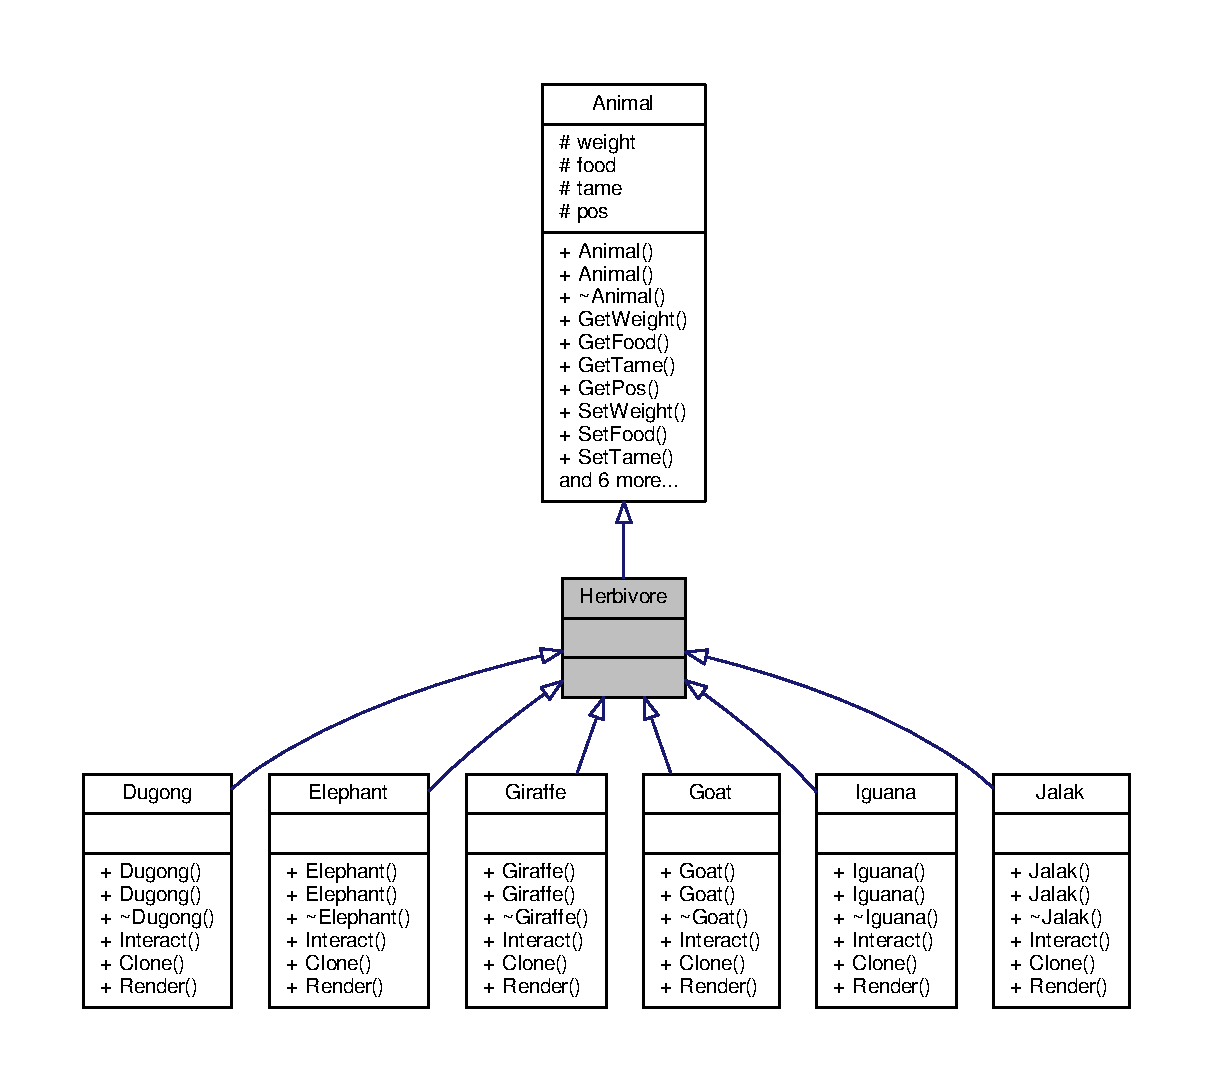
\includegraphics[width=350pt]{classHerbivore__inherit__graph}
\end{center}
\end{figure}


Collaboration diagram for Herbivore\+:
\nopagebreak
\begin{figure}[H]
\begin{center}
\leavevmode
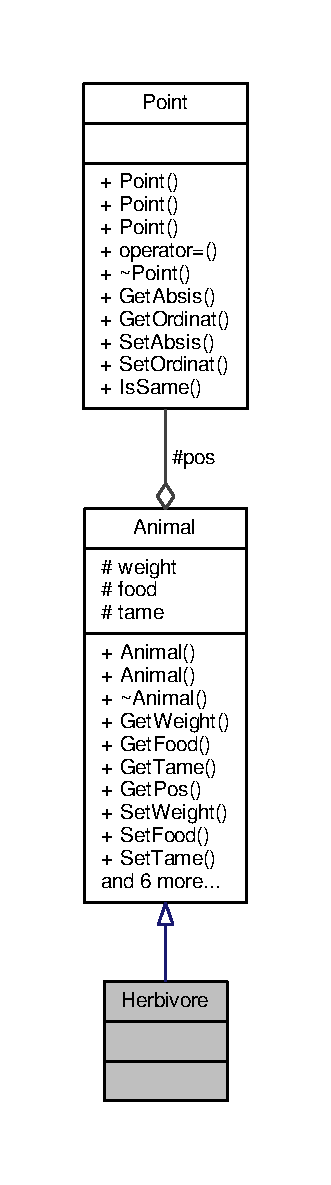
\includegraphics[height=550pt]{classHerbivore__coll__graph}
\end{center}
\end{figure}
\subsection*{Additional Inherited Members}


\subsection{Detailed Description}
Kelas abstrak \hyperlink{classHerbivore}{Herbivore} merupakan kelas bagi animal pemakan tumbuhan 

The documentation for this class was generated from the following file\+:\begin{DoxyCompactItemize}
\item 
herbivore/\hyperlink{herbivore_8h}{herbivore.\+h}\end{DoxyCompactItemize}

\hypertarget{classIguana}{}\section{Iguana Class Reference}
\label{classIguana}\index{Iguana@{Iguana}}


{\ttfamily \#include $<$iguana.\+h$>$}



Inheritance diagram for Iguana\+:
% FIG 0


Collaboration diagram for Iguana\+:
% FIG 1
\subsection*{Public Member Functions}
\begin{DoxyCompactItemize}
\item 
\hyperlink{classIguana_aadc10a5bb8364d915bfd1d3d8ab3156a}{Iguana} ()
\begin{DoxyCompactList}\small\item\em Constructor. Menciptakan objek \hyperlink{classIguana}{Iguana}. \end{DoxyCompactList}\item 
virtual \hyperlink{classIguana_af0a4082cc22aea6f76f42c859d9375ad}{$\sim$\+Iguana} ()
\begin{DoxyCompactList}\small\item\em Destructor. \end{DoxyCompactList}\item 
string \hyperlink{classIguana_a271ef320fd3d4973e50e89aa30cffe3e}{Interact} ()
\begin{DoxyCompactList}\small\item\em Interaksi yang dilakukan \hyperlink{classIguana}{Iguana}. \end{DoxyCompactList}\item 
virtual \hyperlink{classIguana}{Iguana} $\ast$ \hyperlink{classIguana_a40e56fb855d09d2a8788dc73e2fdfc8a}{Clone} () const 
\begin{DoxyCompactList}\small\item\em Melakukan cloning untuk menciptakan objek \hyperlink{classIguana}{Iguana} baru. \end{DoxyCompactList}\item 
char \hyperlink{classIguana_a18bbb71a80e6b2a9855623b1c7f108b9}{Render} ()
\begin{DoxyCompactList}\small\item\em Render dari \hyperlink{classIguana}{Iguana}. \end{DoxyCompactList}\end{DoxyCompactItemize}
\subsection*{Additional Inherited Members}


\subsection{Detailed Description}
kelas \hyperlink{classIguana}{Iguana} merupakan kelas untuk real object \hyperlink{classIguana}{Iguana} 

\subsection{Constructor \& Destructor Documentation}
\index{Iguana@{Iguana}!Iguana@{Iguana}}
\index{Iguana@{Iguana}!Iguana@{Iguana}}
\subsubsection[{\texorpdfstring{Iguana()}{Iguana()}}]{\setlength{\rightskip}{0pt plus 5cm}Iguana\+::\+Iguana (
\begin{DoxyParamCaption}
{}
\end{DoxyParamCaption}
)\hspace{0.3cm}{\ttfamily [inline]}}\hypertarget{classIguana_aadc10a5bb8364d915bfd1d3d8ab3156a}{}\label{classIguana_aadc10a5bb8364d915bfd1d3d8ab3156a}


Constructor. Menciptakan objek \hyperlink{classIguana}{Iguana}. 

\index{Iguana@{Iguana}!````~Iguana@{$\sim$\+Iguana}}
\index{````~Iguana@{$\sim$\+Iguana}!Iguana@{Iguana}}
\subsubsection[{\texorpdfstring{$\sim$\+Iguana()}{~Iguana()}}]{\setlength{\rightskip}{0pt plus 5cm}virtual Iguana\+::$\sim$\+Iguana (
\begin{DoxyParamCaption}
{}
\end{DoxyParamCaption}
)\hspace{0.3cm}{\ttfamily [inline]}, {\ttfamily [virtual]}}\hypertarget{classIguana_af0a4082cc22aea6f76f42c859d9375ad}{}\label{classIguana_af0a4082cc22aea6f76f42c859d9375ad}


Destructor. 



\subsection{Member Function Documentation}
\index{Iguana@{Iguana}!Clone@{Clone}}
\index{Clone@{Clone}!Iguana@{Iguana}}
\subsubsection[{\texorpdfstring{Clone() const }{Clone() const }}]{\setlength{\rightskip}{0pt plus 5cm}virtual {\bf Iguana}$\ast$ Iguana\+::\+Clone (
\begin{DoxyParamCaption}
{}
\end{DoxyParamCaption}
) const\hspace{0.3cm}{\ttfamily [inline]}, {\ttfamily [virtual]}}\hypertarget{classIguana_a40e56fb855d09d2a8788dc73e2fdfc8a}{}\label{classIguana_a40e56fb855d09d2a8788dc73e2fdfc8a}


Melakukan cloning untuk menciptakan objek \hyperlink{classIguana}{Iguana} baru. 

\begin{DoxyReturn}{Returns}
Mengembalikan pointer to \hyperlink{classIguana}{Iguana} objek tersebut. 
\end{DoxyReturn}


Implements \hyperlink{classAnimal_a3fc95e2a588b653b9b315e6c7a29c89f}{Animal}.

\index{Iguana@{Iguana}!Interact@{Interact}}
\index{Interact@{Interact}!Iguana@{Iguana}}
\subsubsection[{\texorpdfstring{Interact()}{Interact()}}]{\setlength{\rightskip}{0pt plus 5cm}string Iguana\+::\+Interact (
\begin{DoxyParamCaption}
{}
\end{DoxyParamCaption}
)\hspace{0.3cm}{\ttfamily [inline]}, {\ttfamily [virtual]}}\hypertarget{classIguana_a271ef320fd3d4973e50e89aa30cffe3e}{}\label{classIguana_a271ef320fd3d4973e50e89aa30cffe3e}


Interaksi yang dilakukan \hyperlink{classIguana}{Iguana}. 

\begin{DoxyReturn}{Returns}
Mengembalikan string yang merepresentasikan suara \hyperlink{classIguana}{Iguana}. 
\end{DoxyReturn}


Implements \hyperlink{classAnimal_ad5a55fb0355a9425fee6611003d9892c}{Animal}.

\index{Iguana@{Iguana}!Render@{Render}}
\index{Render@{Render}!Iguana@{Iguana}}
\subsubsection[{\texorpdfstring{Render()}{Render()}}]{\setlength{\rightskip}{0pt plus 5cm}char Iguana\+::\+Render (
\begin{DoxyParamCaption}
{}
\end{DoxyParamCaption}
)\hspace{0.3cm}{\ttfamily [inline]}, {\ttfamily [virtual]}}\hypertarget{classIguana_a18bbb71a80e6b2a9855623b1c7f108b9}{}\label{classIguana_a18bbb71a80e6b2a9855623b1c7f108b9}


Render dari \hyperlink{classIguana}{Iguana}. 

\begin{DoxyReturn}{Returns}
Mengembalikan char yang merupakan representasi kode \hyperlink{classIguana}{Iguana}. 
\end{DoxyReturn}


Implements \hyperlink{classAnimal_a43a47c0f41d211128e04abc6add53def}{Animal}.



The documentation for this class was generated from the following file\+:\begin{DoxyCompactItemize}
\item 
iguana/\hyperlink{iguana_8h}{iguana.\+h}\end{DoxyCompactItemize}

\hypertarget{classJalak}{}\section{Jalak Class Reference}
\label{classJalak}\index{Jalak@{Jalak}}


{\ttfamily \#include $<$jalak.\+h$>$}



Inheritance diagram for Jalak\+:
% FIG 0


Collaboration diagram for Jalak\+:
% FIG 1
\subsection*{Public Member Functions}
\begin{DoxyCompactItemize}
\item 
\hyperlink{classJalak_a3887e1118830188e1aeffee215b2816f}{Jalak} ()
\begin{DoxyCompactList}\small\item\em Constructor. Menciptakan objek \hyperlink{classJalak}{Jalak}. \end{DoxyCompactList}\item 
virtual \hyperlink{classJalak_a2c1e4e68ab9126c034520c2c845a5afa}{$\sim$\+Jalak} ()
\begin{DoxyCompactList}\small\item\em Destructor. \end{DoxyCompactList}\item 
string \hyperlink{classJalak_a864b931f04f1580759c4a108e1734bb8}{Interact} ()
\begin{DoxyCompactList}\small\item\em Interaksi yang dilakukan \hyperlink{classJalak}{Jalak}. \end{DoxyCompactList}\item 
virtual \hyperlink{classJalak}{Jalak} $\ast$ \hyperlink{classJalak_a85b145221386cdca75274b4438250161}{Clone} () const 
\begin{DoxyCompactList}\small\item\em Melakukan cloning untuk menciptakan objek \hyperlink{classJalak}{Jalak} baru. \end{DoxyCompactList}\item 
char \hyperlink{classJalak_af500189104401b66d6ab4e3b1106ce74}{Render} ()
\begin{DoxyCompactList}\small\item\em Render dari \hyperlink{classJalak}{Jalak}. \end{DoxyCompactList}\end{DoxyCompactItemize}
\subsection*{Additional Inherited Members}


\subsection{Detailed Description}
Kelas \hyperlink{classJalak}{Jalak} merupakan kelas untuk real object \hyperlink{classJalak}{Jalak} 

\subsection{Constructor \& Destructor Documentation}
\index{Jalak@{Jalak}!Jalak@{Jalak}}
\index{Jalak@{Jalak}!Jalak@{Jalak}}
\subsubsection[{\texorpdfstring{Jalak()}{Jalak()}}]{\setlength{\rightskip}{0pt plus 5cm}Jalak\+::\+Jalak (
\begin{DoxyParamCaption}
{}
\end{DoxyParamCaption}
)\hspace{0.3cm}{\ttfamily [inline]}}\hypertarget{classJalak_a3887e1118830188e1aeffee215b2816f}{}\label{classJalak_a3887e1118830188e1aeffee215b2816f}


Constructor. Menciptakan objek \hyperlink{classJalak}{Jalak}. 

\index{Jalak@{Jalak}!````~Jalak@{$\sim$\+Jalak}}
\index{````~Jalak@{$\sim$\+Jalak}!Jalak@{Jalak}}
\subsubsection[{\texorpdfstring{$\sim$\+Jalak()}{~Jalak()}}]{\setlength{\rightskip}{0pt plus 5cm}virtual Jalak\+::$\sim$\+Jalak (
\begin{DoxyParamCaption}
{}
\end{DoxyParamCaption}
)\hspace{0.3cm}{\ttfamily [inline]}, {\ttfamily [virtual]}}\hypertarget{classJalak_a2c1e4e68ab9126c034520c2c845a5afa}{}\label{classJalak_a2c1e4e68ab9126c034520c2c845a5afa}


Destructor. 



\subsection{Member Function Documentation}
\index{Jalak@{Jalak}!Clone@{Clone}}
\index{Clone@{Clone}!Jalak@{Jalak}}
\subsubsection[{\texorpdfstring{Clone() const }{Clone() const }}]{\setlength{\rightskip}{0pt plus 5cm}virtual {\bf Jalak}$\ast$ Jalak\+::\+Clone (
\begin{DoxyParamCaption}
{}
\end{DoxyParamCaption}
) const\hspace{0.3cm}{\ttfamily [inline]}, {\ttfamily [virtual]}}\hypertarget{classJalak_a85b145221386cdca75274b4438250161}{}\label{classJalak_a85b145221386cdca75274b4438250161}


Melakukan cloning untuk menciptakan objek \hyperlink{classJalak}{Jalak} baru. 

\begin{DoxyReturn}{Returns}
Mengembalikan pointer to \hyperlink{classJalak}{Jalak} objek tersebut. 
\end{DoxyReturn}


Implements \hyperlink{classAnimal_a3fc95e2a588b653b9b315e6c7a29c89f}{Animal}.

\index{Jalak@{Jalak}!Interact@{Interact}}
\index{Interact@{Interact}!Jalak@{Jalak}}
\subsubsection[{\texorpdfstring{Interact()}{Interact()}}]{\setlength{\rightskip}{0pt plus 5cm}string Jalak\+::\+Interact (
\begin{DoxyParamCaption}
{}
\end{DoxyParamCaption}
)\hspace{0.3cm}{\ttfamily [inline]}, {\ttfamily [virtual]}}\hypertarget{classJalak_a864b931f04f1580759c4a108e1734bb8}{}\label{classJalak_a864b931f04f1580759c4a108e1734bb8}


Interaksi yang dilakukan \hyperlink{classJalak}{Jalak}. 

\begin{DoxyReturn}{Returns}
Mengembalikan string yang merepresentasikan suara \hyperlink{classJalak}{Jalak}. 
\end{DoxyReturn}


Implements \hyperlink{classAnimal_ad5a55fb0355a9425fee6611003d9892c}{Animal}.

\index{Jalak@{Jalak}!Render@{Render}}
\index{Render@{Render}!Jalak@{Jalak}}
\subsubsection[{\texorpdfstring{Render()}{Render()}}]{\setlength{\rightskip}{0pt plus 5cm}char Jalak\+::\+Render (
\begin{DoxyParamCaption}
{}
\end{DoxyParamCaption}
)\hspace{0.3cm}{\ttfamily [inline]}, {\ttfamily [virtual]}}\hypertarget{classJalak_af500189104401b66d6ab4e3b1106ce74}{}\label{classJalak_af500189104401b66d6ab4e3b1106ce74}


Render dari \hyperlink{classJalak}{Jalak}. 

\begin{DoxyReturn}{Returns}
Mengembalikan char yang merupakan representasi kode \hyperlink{classJalak}{Jalak}. 
\end{DoxyReturn}


Implements \hyperlink{classAnimal_a43a47c0f41d211128e04abc6add53def}{Animal}.



The documentation for this class was generated from the following file\+:\begin{DoxyCompactItemize}
\item 
jalak/\hyperlink{jalak_8h}{jalak.\+h}\end{DoxyCompactItemize}

\hypertarget{classDriver_1_1Kelas}{}\section{Driver\+:\+:Kelas Class Reference}
\label{classDriver_1_1Kelas}\index{Driver\+::\+Kelas@{Driver\+::\+Kelas}}


Collaboration diagram for Driver\+:\+:Kelas\+:
\nopagebreak
\begin{figure}[H]
\begin{center}
\leavevmode
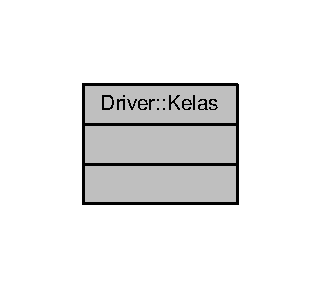
\includegraphics[width=154pt]{classDriver_1_1Kelas__coll__graph}
\end{center}
\end{figure}


\subsection{Detailed Description}
kelas sebagai pilihan menu aplikasi. 

The documentation for this class was generated from the following file\+:\begin{DoxyCompactItemize}
\item 
driver/\hyperlink{driver_8h}{driver.\+h}\end{DoxyCompactItemize}

\hypertarget{classCage_1_1Kelas}{}\section{Cage\+:\+:Kelas Class Reference}
\label{classCage_1_1Kelas}\index{Cage\+::\+Kelas@{Cage\+::\+Kelas}}


Collaboration diagram for Cage\+:\+:Kelas\+:
% FIG 0


\subsection{Detailed Description}
himpunan \hyperlink{classCell}{Cell} yang bertipe sama. 

The documentation for this class was generated from the following file\+:\begin{DoxyCompactItemize}
\item 
cage/\hyperlink{cage_8h}{cage.\+h}\end{DoxyCompactItemize}

\hypertarget{classCell_1_1Kelas}{}\section{Cell\+:\+:Kelas Class Reference}
\label{classCell_1_1Kelas}\index{Cell\+::\+Kelas@{Cell\+::\+Kelas}}


Collaboration diagram for Cell\+:\+:Kelas\+:\nopagebreak
\begin{figure}[H]
\begin{center}
\leavevmode
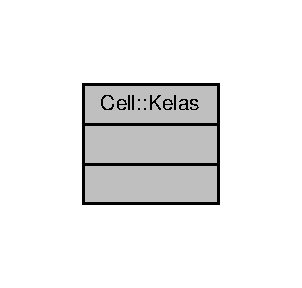
\includegraphics[width=145pt]{classCell_1_1Kelas__coll__graph}
\end{center}
\end{figure}


\subsection{Detailed Description}
simulasi dari petak-\/petak yang terdapat dalam kebun binatang. 

The documentation for this class was generated from the following file\+:\begin{DoxyCompactItemize}
\item 
cell/\hyperlink{cell_8h}{cell.\+h}\end{DoxyCompactItemize}

\hypertarget{classKomodo}{}\section{Komodo Class Reference}
\label{classKomodo}\index{Komodo@{Komodo}}


{\ttfamily \#include $<$komodo.\+h$>$}



Inheritance diagram for Komodo\+:
\nopagebreak
\begin{figure}[H]
\begin{center}
\leavevmode
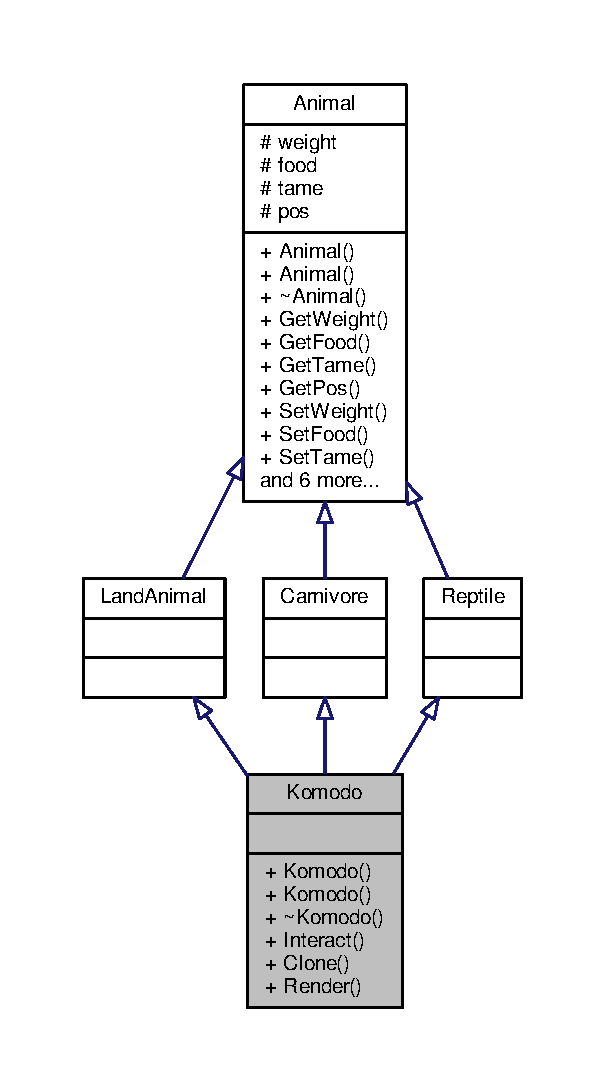
\includegraphics[width=291pt]{classKomodo__inherit__graph}
\end{center}
\end{figure}


Collaboration diagram for Komodo\+:
\nopagebreak
\begin{figure}[H]
\begin{center}
\leavevmode
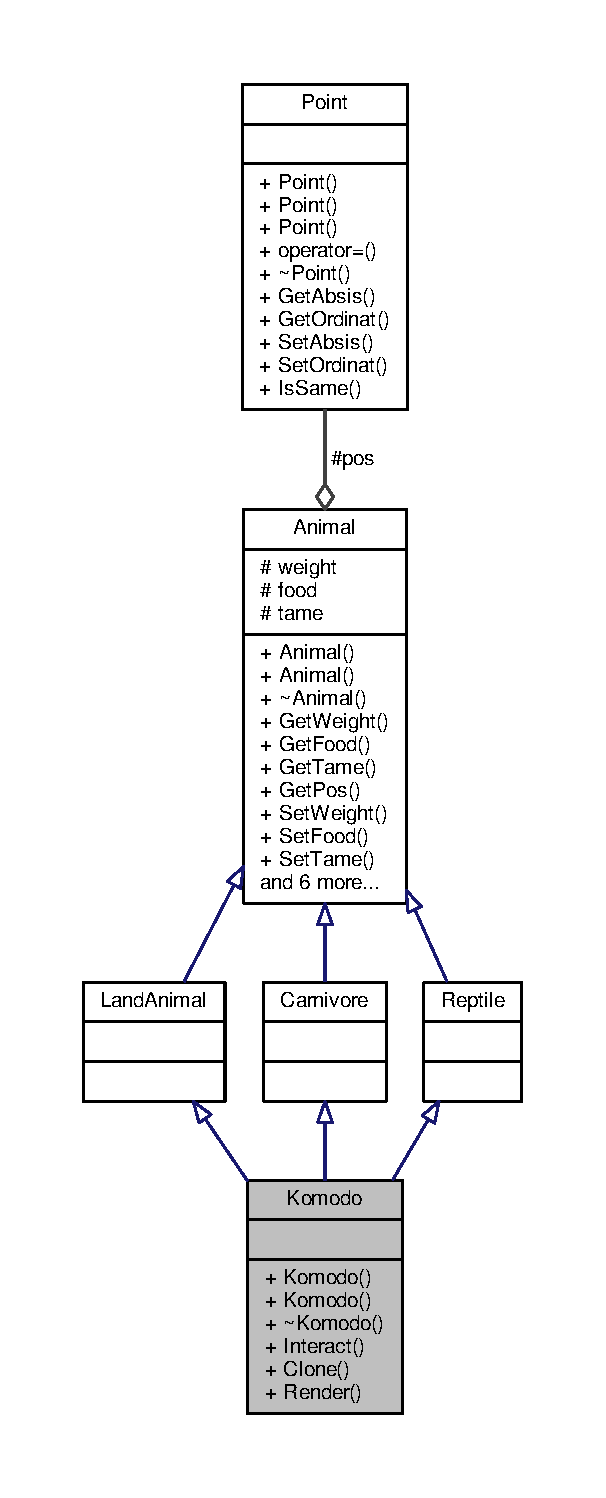
\includegraphics[height=550pt]{classKomodo__coll__graph}
\end{center}
\end{figure}
\subsection*{Public Member Functions}
\begin{DoxyCompactItemize}
\item 
\hyperlink{classKomodo_a663a1a18bc7ac367f1a55a385604258d}{Komodo} ()
\begin{DoxyCompactList}\small\item\em Constructor. Menciptakan objek \hyperlink{classKomodo}{Komodo}. \end{DoxyCompactList}\item 
\hyperlink{classKomodo_ad98e389b1661efeeba847133e64c02e6}{Komodo} (float w, float f, bool t)
\begin{DoxyCompactList}\small\item\em Constructor dengan parameter. Menciptakan objek \hyperlink{classKomodo}{Komodo} dengan berat w, jumlah makanan f, dan status jinak t. \end{DoxyCompactList}\item 
virtual \hyperlink{classKomodo_a16e327cbffe1088c1f04c397c1fbc6dd}{$\sim$\+Komodo} ()
\begin{DoxyCompactList}\small\item\em Destructor. \end{DoxyCompactList}\item 
string \hyperlink{classKomodo_a250e6b06c369a94faaa551751cd09196}{Interact} ()
\begin{DoxyCompactList}\small\item\em interact \end{DoxyCompactList}\item 
virtual \hyperlink{classKomodo}{Komodo} $\ast$ \hyperlink{classKomodo_aab3bd7ee8235c87e8bbafd8848968be8}{Clone} () const 
\begin{DoxyCompactList}\small\item\em Melakukan cloning untuk menciptakan objek \hyperlink{classKomodo}{Komodo} baru. \end{DoxyCompactList}\item 
char \hyperlink{classKomodo_a06ce8ed3d58a33968ecf4a12a3ebbd4d}{Render} ()
\begin{DoxyCompactList}\small\item\em render \end{DoxyCompactList}\end{DoxyCompactItemize}
\subsection*{Additional Inherited Members}


\subsection{Detailed Description}
Kelas \hyperlink{classKomodo}{Komodo} merupakan kelas untuk real object \hyperlink{classKomodo}{Komodo} 

\subsection{Constructor \& Destructor Documentation}
\index{Komodo@{Komodo}!Komodo@{Komodo}}
\index{Komodo@{Komodo}!Komodo@{Komodo}}
\subsubsection[{\texorpdfstring{Komodo()}{Komodo()}}]{\setlength{\rightskip}{0pt plus 5cm}Komodo\+::\+Komodo (
\begin{DoxyParamCaption}
{}
\end{DoxyParamCaption}
)\hspace{0.3cm}{\ttfamily [inline]}}\hypertarget{classKomodo_a663a1a18bc7ac367f1a55a385604258d}{}\label{classKomodo_a663a1a18bc7ac367f1a55a385604258d}


Constructor. Menciptakan objek \hyperlink{classKomodo}{Komodo}. 

\index{Komodo@{Komodo}!Komodo@{Komodo}}
\index{Komodo@{Komodo}!Komodo@{Komodo}}
\subsubsection[{\texorpdfstring{Komodo(float w, float f, bool t)}{Komodo(float w, float f, bool t)}}]{\setlength{\rightskip}{0pt plus 5cm}Komodo\+::\+Komodo (
\begin{DoxyParamCaption}
\item[{float}]{w, }
\item[{float}]{f, }
\item[{bool}]{t}
\end{DoxyParamCaption}
)\hspace{0.3cm}{\ttfamily [inline]}}\hypertarget{classKomodo_ad98e389b1661efeeba847133e64c02e6}{}\label{classKomodo_ad98e389b1661efeeba847133e64c02e6}


Constructor dengan parameter. Menciptakan objek \hyperlink{classKomodo}{Komodo} dengan berat w, jumlah makanan f, dan status jinak t. 


\begin{DoxyParams}{Parameters}
{\em w} & Berat \hyperlink{classKomodo}{Komodo}. \\
\hline
{\em k} & Jumlah makanan \hyperlink{classKomodo}{Komodo}. \\
\hline
{\em t} & Status jinak \hyperlink{classKomodo}{Komodo}. \\
\hline
\end{DoxyParams}
\index{Komodo@{Komodo}!````~Komodo@{$\sim$\+Komodo}}
\index{````~Komodo@{$\sim$\+Komodo}!Komodo@{Komodo}}
\subsubsection[{\texorpdfstring{$\sim$\+Komodo()}{~Komodo()}}]{\setlength{\rightskip}{0pt plus 5cm}virtual Komodo\+::$\sim$\+Komodo (
\begin{DoxyParamCaption}
{}
\end{DoxyParamCaption}
)\hspace{0.3cm}{\ttfamily [inline]}, {\ttfamily [virtual]}}\hypertarget{classKomodo_a16e327cbffe1088c1f04c397c1fbc6dd}{}\label{classKomodo_a16e327cbffe1088c1f04c397c1fbc6dd}


Destructor. 



\subsection{Member Function Documentation}
\index{Komodo@{Komodo}!Clone@{Clone}}
\index{Clone@{Clone}!Komodo@{Komodo}}
\subsubsection[{\texorpdfstring{Clone() const }{Clone() const }}]{\setlength{\rightskip}{0pt plus 5cm}virtual {\bf Komodo}$\ast$ Komodo\+::\+Clone (
\begin{DoxyParamCaption}
{}
\end{DoxyParamCaption}
) const\hspace{0.3cm}{\ttfamily [inline]}, {\ttfamily [virtual]}}\hypertarget{classKomodo_aab3bd7ee8235c87e8bbafd8848968be8}{}\label{classKomodo_aab3bd7ee8235c87e8bbafd8848968be8}


Melakukan cloning untuk menciptakan objek \hyperlink{classKomodo}{Komodo} baru. 

\begin{DoxyReturn}{Returns}
Mengembalikan pointer to \hyperlink{classKomodo}{Komodo} objek tersebut. 
\end{DoxyReturn}


Implements \hyperlink{classAnimal_a3fc95e2a588b653b9b315e6c7a29c89f}{Animal}.

\index{Komodo@{Komodo}!Interact@{Interact}}
\index{Interact@{Interact}!Komodo@{Komodo}}
\subsubsection[{\texorpdfstring{Interact()}{Interact()}}]{\setlength{\rightskip}{0pt plus 5cm}string Komodo\+::\+Interact (
\begin{DoxyParamCaption}
{}
\end{DoxyParamCaption}
)\hspace{0.3cm}{\ttfamily [inline]}, {\ttfamily [virtual]}}\hypertarget{classKomodo_a250e6b06c369a94faaa551751cd09196}{}\label{classKomodo_a250e6b06c369a94faaa551751cd09196}


interact 

\begin{DoxyReturn}{Returns}
Mengembalikan string yang merepresentasikan suara \hyperlink{classKomodo}{Komodo}. 
\end{DoxyReturn}


Implements \hyperlink{classAnimal_ad5a55fb0355a9425fee6611003d9892c}{Animal}.

\index{Komodo@{Komodo}!Render@{Render}}
\index{Render@{Render}!Komodo@{Komodo}}
\subsubsection[{\texorpdfstring{Render()}{Render()}}]{\setlength{\rightskip}{0pt plus 5cm}char Komodo\+::\+Render (
\begin{DoxyParamCaption}
{}
\end{DoxyParamCaption}
)\hspace{0.3cm}{\ttfamily [inline]}, {\ttfamily [virtual]}}\hypertarget{classKomodo_a06ce8ed3d58a33968ecf4a12a3ebbd4d}{}\label{classKomodo_a06ce8ed3d58a33968ecf4a12a3ebbd4d}


render 

\begin{DoxyReturn}{Returns}
Mengembalikan char yang merupakan representasi kode \hyperlink{classKomodo}{Komodo}. 
\end{DoxyReturn}


Implements \hyperlink{classAnimal_a43a47c0f41d211128e04abc6add53def}{Animal}.



The documentation for this class was generated from the following file\+:\begin{DoxyCompactItemize}
\item 
\hyperlink{komodo_8h}{komodo.\+h}\end{DoxyCompactItemize}

\hypertarget{classLandAnimal}{}\section{Land\+Animal Class Reference}
\label{classLandAnimal}\index{Land\+Animal@{Land\+Animal}}


{\ttfamily \#include $<$land\+\_\+animal.\+h$>$}



Inheritance diagram for Land\+Animal\+:
\nopagebreak
\begin{figure}[H]
\begin{center}
\leavevmode
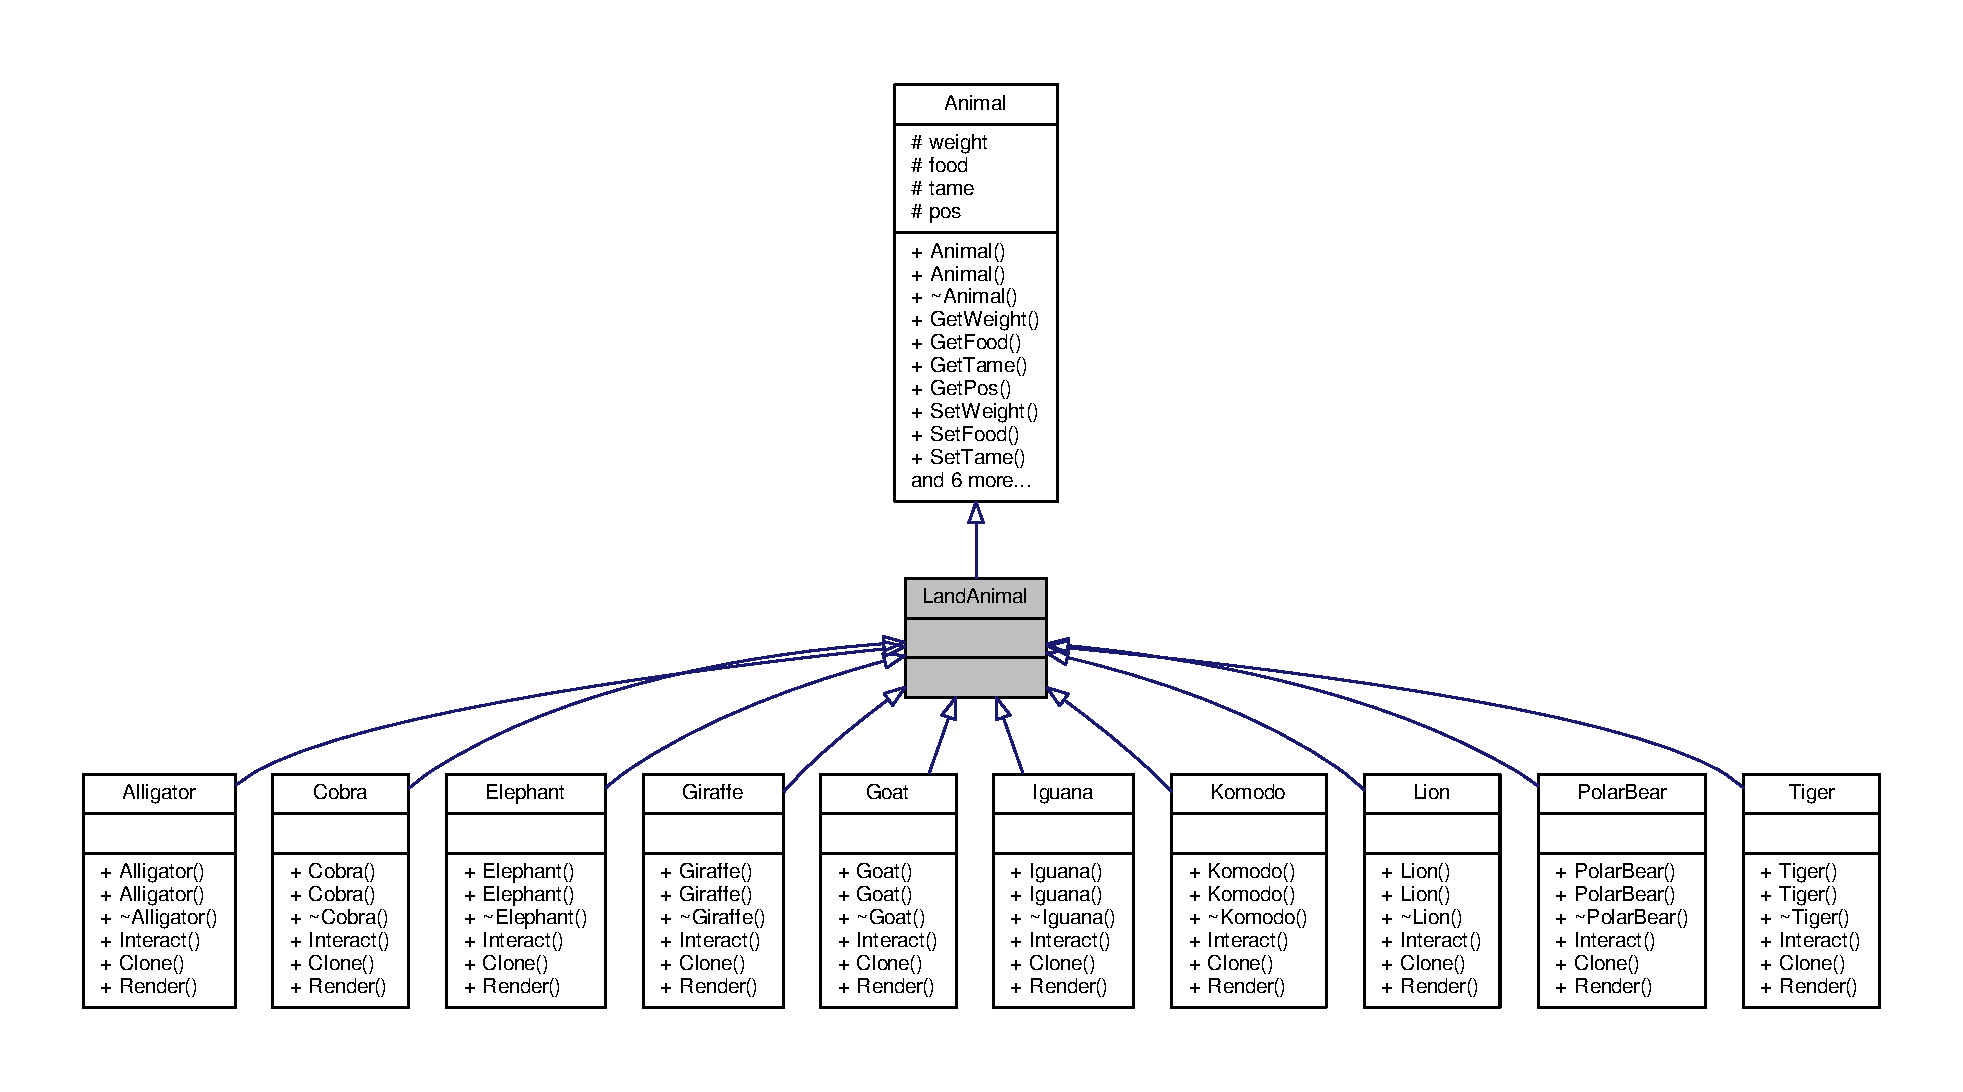
\includegraphics[width=350pt]{classLandAnimal__inherit__graph}
\end{center}
\end{figure}


Collaboration diagram for Land\+Animal\+:
\nopagebreak
\begin{figure}[H]
\begin{center}
\leavevmode
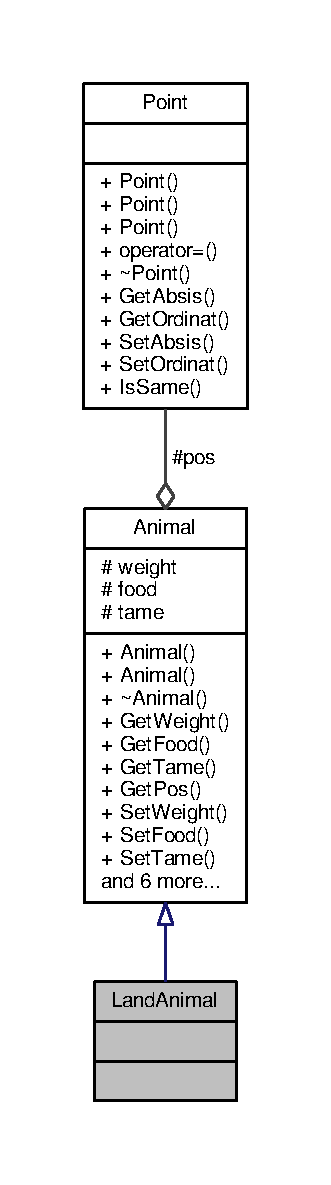
\includegraphics[height=550pt]{classLandAnimal__coll__graph}
\end{center}
\end{figure}
\subsection*{Additional Inherited Members}


\subsection{Detailed Description}
Kelas abstrak \hyperlink{classLandAnimal}{Land\+Animal} merupakan kelas bagi animal dengan habitat di darat 

The documentation for this class was generated from the following file\+:\begin{DoxyCompactItemize}
\item 
\hyperlink{land__animal_8h}{land\+\_\+animal.\+h}\end{DoxyCompactItemize}

\hypertarget{classLandHabitat}{}\section{Land\+Habitat Class Reference}
\label{classLandHabitat}\index{Land\+Habitat@{Land\+Habitat}}


{\ttfamily \#include $<$land\+\_\+habitat.\+h$>$}



Inheritance diagram for Land\+Habitat\+:
\nopagebreak
\begin{figure}[H]
\begin{center}
\leavevmode
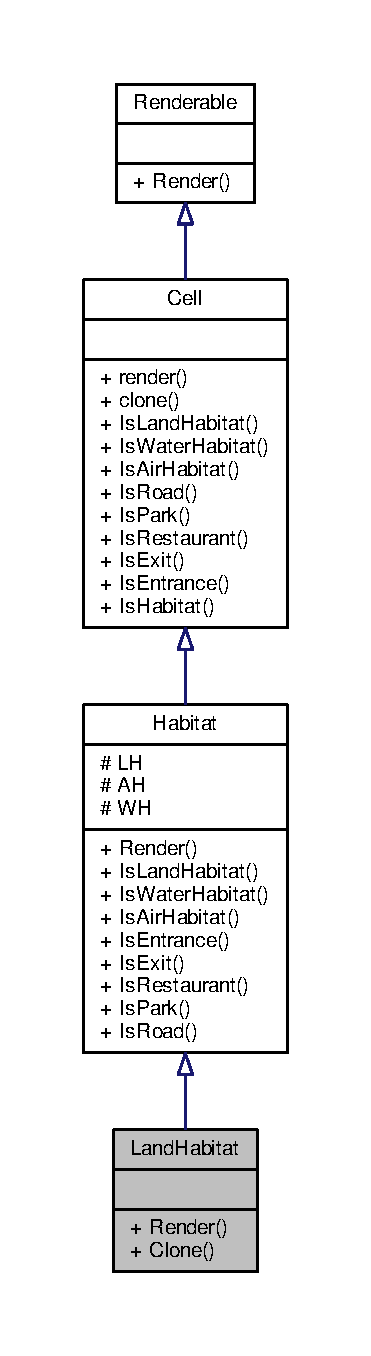
\includegraphics[height=550pt]{classLandHabitat__inherit__graph}
\end{center}
\end{figure}


Collaboration diagram for Land\+Habitat\+:
\nopagebreak
\begin{figure}[H]
\begin{center}
\leavevmode
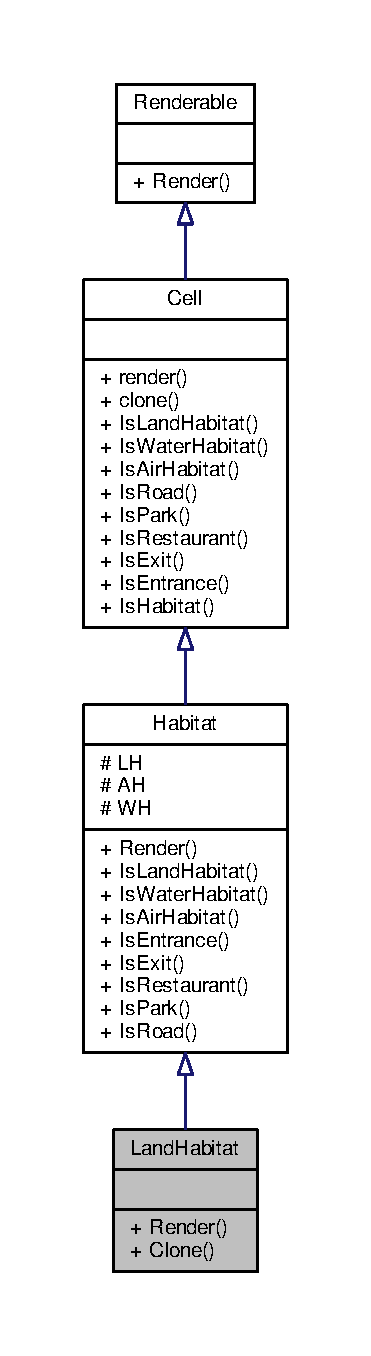
\includegraphics[height=550pt]{classLandHabitat__coll__graph}
\end{center}
\end{figure}
\subsection*{Public Member Functions}
\begin{DoxyCompactItemize}
\item 
char \hyperlink{classLandHabitat_ad2147498f493b01429ae315f0145d3a9}{Render} ()
\begin{DoxyCompactList}\small\item\em Render dari \hyperlink{classLandHabitat}{Land\+Habitat}. \end{DoxyCompactList}\item 
virtual \hyperlink{classLandHabitat}{Land\+Habitat} $\ast$ \hyperlink{classLandHabitat_a8cd927afc8d52a9fb8cdc5701893ad81}{Clone} () const 
\begin{DoxyCompactList}\small\item\em Melakukan cloning untuk menciptakan objek \hyperlink{classLandHabitat}{Land\+Habitat} baru. \end{DoxyCompactList}\end{DoxyCompactItemize}
\subsection*{Additional Inherited Members}


\subsection{Detailed Description}
Kelas real \hyperlink{classLandHabitat}{Land\+Habitat} merupakan simulasi dari habitat darat 

\subsection{Member Function Documentation}
\index{Land\+Habitat@{Land\+Habitat}!Clone@{Clone}}
\index{Clone@{Clone}!Land\+Habitat@{Land\+Habitat}}
\subsubsection[{\texorpdfstring{Clone() const }{Clone() const }}]{\setlength{\rightskip}{0pt plus 5cm}virtual {\bf Land\+Habitat}$\ast$ Land\+Habitat\+::\+Clone (
\begin{DoxyParamCaption}
{}
\end{DoxyParamCaption}
) const\hspace{0.3cm}{\ttfamily [inline]}, {\ttfamily [virtual]}}\hypertarget{classLandHabitat_a8cd927afc8d52a9fb8cdc5701893ad81}{}\label{classLandHabitat_a8cd927afc8d52a9fb8cdc5701893ad81}


Melakukan cloning untuk menciptakan objek \hyperlink{classLandHabitat}{Land\+Habitat} baru. 

\begin{DoxyReturn}{Returns}
Mengembalikan pointer to \hyperlink{classLandHabitat}{Land\+Habitat} objek tersebut. 
\end{DoxyReturn}


Implements \hyperlink{classCell_aaa64e56d1ecf0d0a390f2400c189b169}{Cell}.

\index{Land\+Habitat@{Land\+Habitat}!Render@{Render}}
\index{Render@{Render}!Land\+Habitat@{Land\+Habitat}}
\subsubsection[{\texorpdfstring{Render()}{Render()}}]{\setlength{\rightskip}{0pt plus 5cm}char Land\+Habitat\+::\+Render (
\begin{DoxyParamCaption}
{}
\end{DoxyParamCaption}
)\hspace{0.3cm}{\ttfamily [inline]}, {\ttfamily [virtual]}}\hypertarget{classLandHabitat_ad2147498f493b01429ae315f0145d3a9}{}\label{classLandHabitat_ad2147498f493b01429ae315f0145d3a9}


Render dari \hyperlink{classLandHabitat}{Land\+Habitat}. 

\begin{DoxyReturn}{Returns}
Mengembalikan char yang merupakan representasi kode \hyperlink{classLandHabitat}{Land\+Habitat}. 
\end{DoxyReturn}


Implements \hyperlink{classHabitat_ad1bf10205d38e8e308eb9acc3aa2872c}{Habitat}.



The documentation for this class was generated from the following file\+:\begin{DoxyCompactItemize}
\item 
land\+\_\+habitat/\hyperlink{land__habitat_8h}{land\+\_\+habitat.\+h}\end{DoxyCompactItemize}

\hypertarget{classLion}{}\section{Lion Class Reference}
\label{classLion}\index{Lion@{Lion}}


{\ttfamily \#include $<$lion.\+h$>$}



Inheritance diagram for Lion\+:
\nopagebreak
\begin{figure}[H]
\begin{center}
\leavevmode
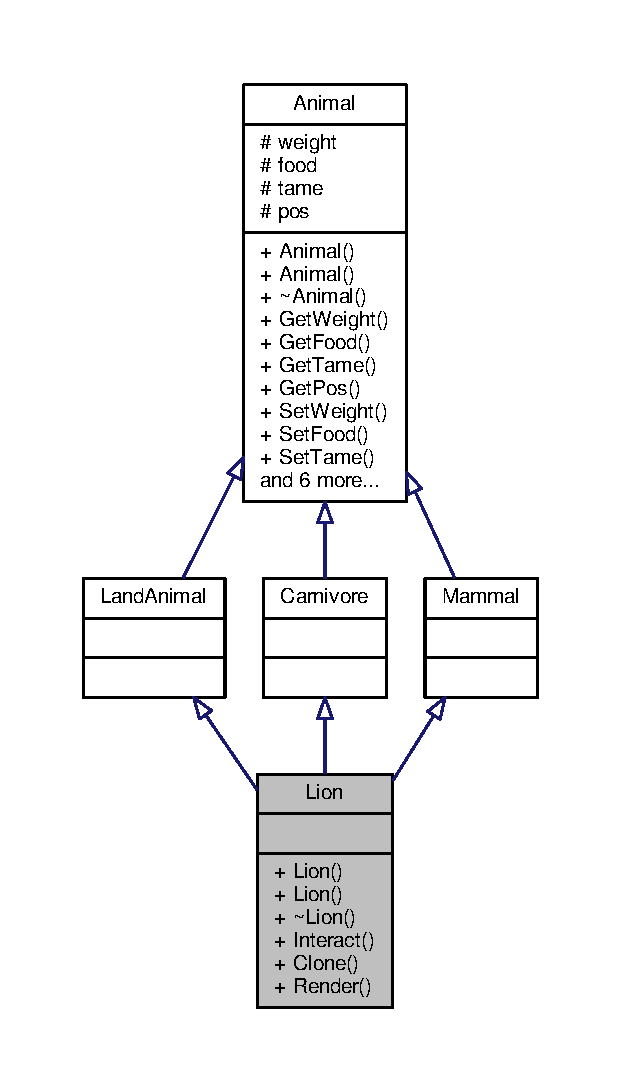
\includegraphics[width=298pt]{classLion__inherit__graph}
\end{center}
\end{figure}


Collaboration diagram for Lion\+:
\nopagebreak
\begin{figure}[H]
\begin{center}
\leavevmode
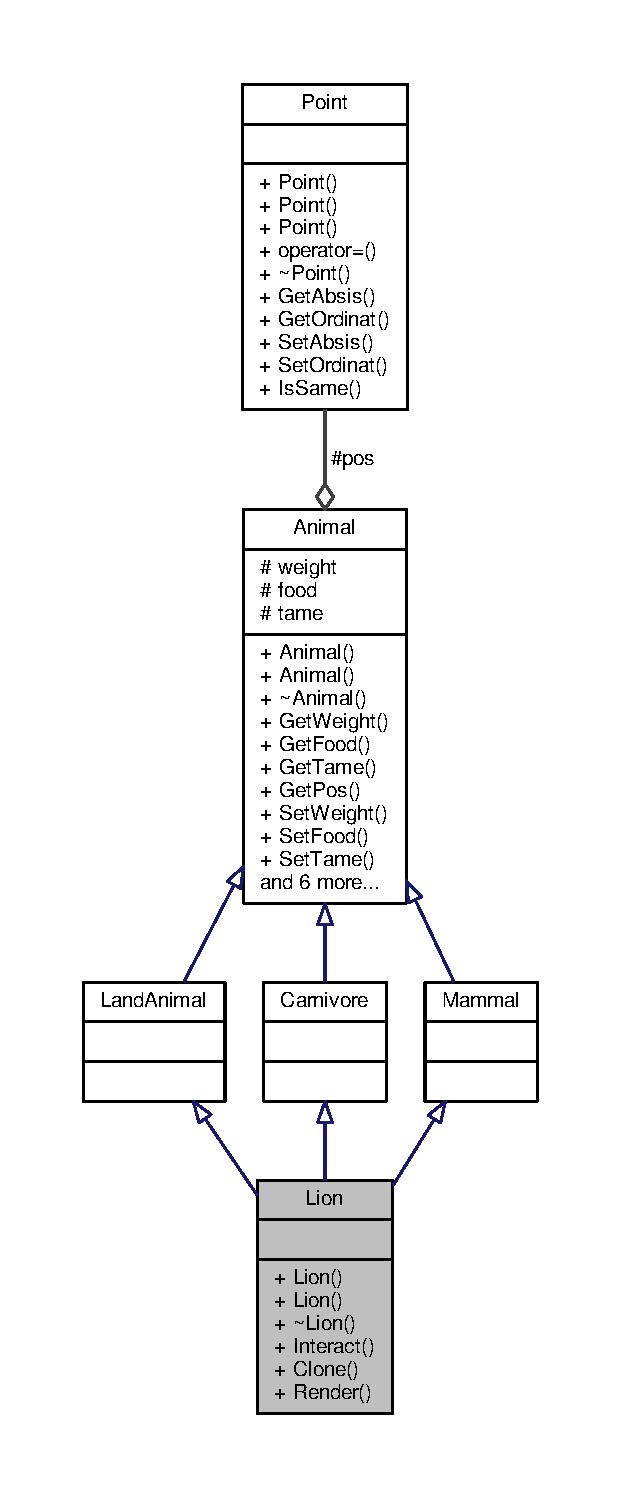
\includegraphics[height=550pt]{classLion__coll__graph}
\end{center}
\end{figure}
\subsection*{Public Member Functions}
\begin{DoxyCompactItemize}
\item 
\hyperlink{classLion_a582202364024a9ce10e57f47c872dbc2}{Lion} ()
\begin{DoxyCompactList}\small\item\em Constructor. Menciptakan objek \hyperlink{classLion}{Lion}. \end{DoxyCompactList}\item 
\hyperlink{classLion_a5bc46f23f72bc31fe8ef58db40a62b58}{Lion} (float w, float f, bool t)
\begin{DoxyCompactList}\small\item\em Constructor dengan parameter. Menciptakan objek \hyperlink{classLion}{Lion} dengan berat w, jumlah makanan f, dan status jinak t. \end{DoxyCompactList}\item 
virtual \hyperlink{classLion_a09c9c113e6ca2d7c7b304b009d61dc62}{$\sim$\+Lion} ()
\begin{DoxyCompactList}\small\item\em Destructor. \end{DoxyCompactList}\item 
string \hyperlink{classLion_a4c090a9b5f42b92c30d223b40435e167}{Interact} ()
\begin{DoxyCompactList}\small\item\em interact \end{DoxyCompactList}\item 
virtual \hyperlink{classLion}{Lion} $\ast$ \hyperlink{classLion_ae63405ef106650644a8fcafc7393284e}{Clone} () const 
\begin{DoxyCompactList}\small\item\em Melakukan cloning untuk menciptakan objek \hyperlink{classLion}{Lion} baru. \end{DoxyCompactList}\item 
char \hyperlink{classLion_ad782de7c88e4a7aad01287a2ed64827c}{Render} ()
\begin{DoxyCompactList}\small\item\em render \end{DoxyCompactList}\end{DoxyCompactItemize}
\subsection*{Additional Inherited Members}


\subsection{Detailed Description}
Kelas \hyperlink{classLion}{Lion} merupakan kelas untuk real object \hyperlink{classLion}{Lion} 

\subsection{Constructor \& Destructor Documentation}
\index{Lion@{Lion}!Lion@{Lion}}
\index{Lion@{Lion}!Lion@{Lion}}
\subsubsection[{\texorpdfstring{Lion()}{Lion()}}]{\setlength{\rightskip}{0pt plus 5cm}Lion\+::\+Lion (
\begin{DoxyParamCaption}
{}
\end{DoxyParamCaption}
)\hspace{0.3cm}{\ttfamily [inline]}}\hypertarget{classLion_a582202364024a9ce10e57f47c872dbc2}{}\label{classLion_a582202364024a9ce10e57f47c872dbc2}


Constructor. Menciptakan objek \hyperlink{classLion}{Lion}. 

\index{Lion@{Lion}!Lion@{Lion}}
\index{Lion@{Lion}!Lion@{Lion}}
\subsubsection[{\texorpdfstring{Lion(float w, float f, bool t)}{Lion(float w, float f, bool t)}}]{\setlength{\rightskip}{0pt plus 5cm}Lion\+::\+Lion (
\begin{DoxyParamCaption}
\item[{float}]{w, }
\item[{float}]{f, }
\item[{bool}]{t}
\end{DoxyParamCaption}
)\hspace{0.3cm}{\ttfamily [inline]}}\hypertarget{classLion_a5bc46f23f72bc31fe8ef58db40a62b58}{}\label{classLion_a5bc46f23f72bc31fe8ef58db40a62b58}


Constructor dengan parameter. Menciptakan objek \hyperlink{classLion}{Lion} dengan berat w, jumlah makanan f, dan status jinak t. 


\begin{DoxyParams}{Parameters}
{\em w} & Berat \hyperlink{classLion}{Lion}. \\
\hline
{\em k} & Jumlah makanan \hyperlink{classLion}{Lion}. \\
\hline
{\em t} & Status jinak \hyperlink{classLion}{Lion}. \\
\hline
\end{DoxyParams}
\index{Lion@{Lion}!````~Lion@{$\sim$\+Lion}}
\index{````~Lion@{$\sim$\+Lion}!Lion@{Lion}}
\subsubsection[{\texorpdfstring{$\sim$\+Lion()}{~Lion()}}]{\setlength{\rightskip}{0pt plus 5cm}virtual Lion\+::$\sim$\+Lion (
\begin{DoxyParamCaption}
{}
\end{DoxyParamCaption}
)\hspace{0.3cm}{\ttfamily [inline]}, {\ttfamily [virtual]}}\hypertarget{classLion_a09c9c113e6ca2d7c7b304b009d61dc62}{}\label{classLion_a09c9c113e6ca2d7c7b304b009d61dc62}


Destructor. 



\subsection{Member Function Documentation}
\index{Lion@{Lion}!Clone@{Clone}}
\index{Clone@{Clone}!Lion@{Lion}}
\subsubsection[{\texorpdfstring{Clone() const }{Clone() const }}]{\setlength{\rightskip}{0pt plus 5cm}virtual {\bf Lion}$\ast$ Lion\+::\+Clone (
\begin{DoxyParamCaption}
{}
\end{DoxyParamCaption}
) const\hspace{0.3cm}{\ttfamily [inline]}, {\ttfamily [virtual]}}\hypertarget{classLion_ae63405ef106650644a8fcafc7393284e}{}\label{classLion_ae63405ef106650644a8fcafc7393284e}


Melakukan cloning untuk menciptakan objek \hyperlink{classLion}{Lion} baru. 

\begin{DoxyReturn}{Returns}
Mengembalikan pointer to \hyperlink{classLion}{Lion} objek tersebut. 
\end{DoxyReturn}


Implements \hyperlink{classAnimal_a3fc95e2a588b653b9b315e6c7a29c89f}{Animal}.

\index{Lion@{Lion}!Interact@{Interact}}
\index{Interact@{Interact}!Lion@{Lion}}
\subsubsection[{\texorpdfstring{Interact()}{Interact()}}]{\setlength{\rightskip}{0pt plus 5cm}string Lion\+::\+Interact (
\begin{DoxyParamCaption}
{}
\end{DoxyParamCaption}
)\hspace{0.3cm}{\ttfamily [inline]}, {\ttfamily [virtual]}}\hypertarget{classLion_a4c090a9b5f42b92c30d223b40435e167}{}\label{classLion_a4c090a9b5f42b92c30d223b40435e167}


interact 

\begin{DoxyReturn}{Returns}
Mengembalikan string yang merepresentasikan suara \hyperlink{classLion}{Lion}. 
\end{DoxyReturn}


Implements \hyperlink{classAnimal_ad5a55fb0355a9425fee6611003d9892c}{Animal}.

\index{Lion@{Lion}!Render@{Render}}
\index{Render@{Render}!Lion@{Lion}}
\subsubsection[{\texorpdfstring{Render()}{Render()}}]{\setlength{\rightskip}{0pt plus 5cm}char Lion\+::\+Render (
\begin{DoxyParamCaption}
{}
\end{DoxyParamCaption}
)\hspace{0.3cm}{\ttfamily [inline]}, {\ttfamily [virtual]}}\hypertarget{classLion_ad782de7c88e4a7aad01287a2ed64827c}{}\label{classLion_ad782de7c88e4a7aad01287a2ed64827c}


render 

\begin{DoxyReturn}{Returns}
Mengembalikan char yang merupakan representasi kode \hyperlink{classLion}{Lion}. 
\end{DoxyReturn}


Implements \hyperlink{classAnimal_a43a47c0f41d211128e04abc6add53def}{Animal}.



The documentation for this class was generated from the following file\+:\begin{DoxyCompactItemize}
\item 
\hyperlink{lion_8h}{lion.\+h}\end{DoxyCompactItemize}

\hypertarget{classMammal}{}\section{Mammal Class Reference}
\label{classMammal}\index{Mammal@{Mammal}}


{\ttfamily \#include $<$mammal.\+h$>$}



Inheritance diagram for Mammal\+:
% FIG 0


Collaboration diagram for Mammal\+:
% FIG 1
\subsection*{Additional Inherited Members}


\subsection{Detailed Description}
Kelas abstrak \hyperlink{classMammal}{Mammal} 

The documentation for this class was generated from the following file\+:\begin{DoxyCompactItemize}
\item 
mammal/\hyperlink{mammal_8h}{mammal.\+h}\end{DoxyCompactItemize}

\hypertarget{classOmnivore}{}\section{Omnivore Class Reference}
\label{classOmnivore}\index{Omnivore@{Omnivore}}


{\ttfamily \#include $<$omnivore.\+h$>$}



Inheritance diagram for Omnivore\+:
\nopagebreak
\begin{figure}[H]
\begin{center}
\leavevmode
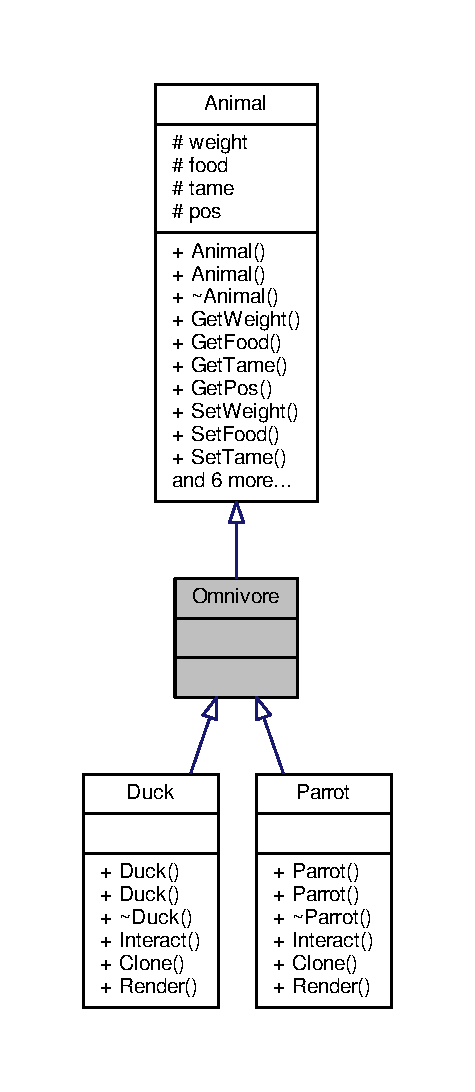
\includegraphics[width=228pt]{classOmnivore__inherit__graph}
\end{center}
\end{figure}


Collaboration diagram for Omnivore\+:
\nopagebreak
\begin{figure}[H]
\begin{center}
\leavevmode
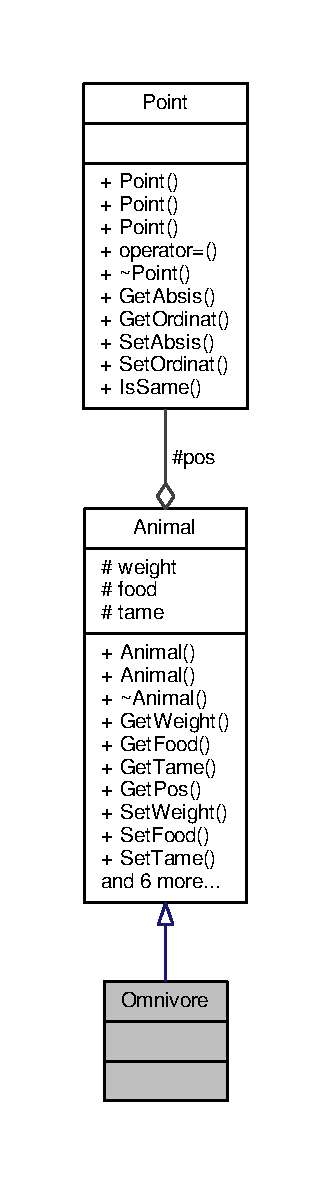
\includegraphics[height=550pt]{classOmnivore__coll__graph}
\end{center}
\end{figure}
\subsection*{Additional Inherited Members}


\subsection{Detailed Description}
Kelas abstrak \hyperlink{classOmnivore}{Omnivore} merupakan kelas abstrak untuk hewan pemakan daging dan tumbuhan 

The documentation for this class was generated from the following file\+:\begin{DoxyCompactItemize}
\item 
omnivore/\hyperlink{omnivore_8h}{omnivore.\+h}\end{DoxyCompactItemize}

\hypertarget{classOrca}{}\section{Orca Class Reference}
\label{classOrca}\index{Orca@{Orca}}


{\ttfamily \#include $<$orca.\+h$>$}



Inheritance diagram for Orca\+:
\nopagebreak
\begin{figure}[H]
\begin{center}
\leavevmode
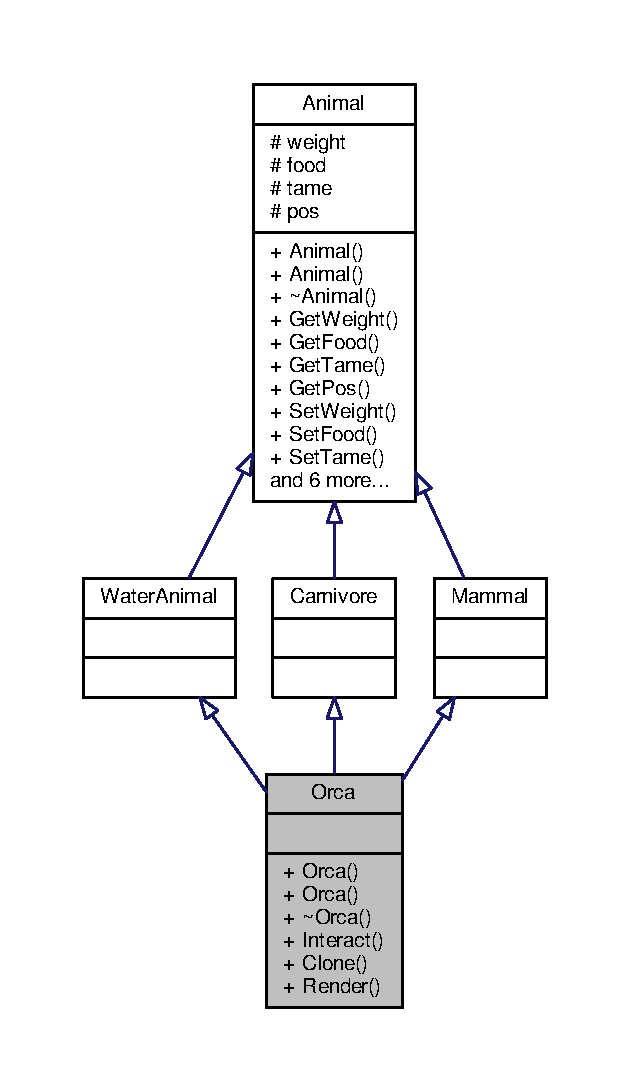
\includegraphics[width=226pt]{classOrca__inherit__graph}
\end{center}
\end{figure}


Collaboration diagram for Orca\+:
\nopagebreak
\begin{figure}[H]
\begin{center}
\leavevmode
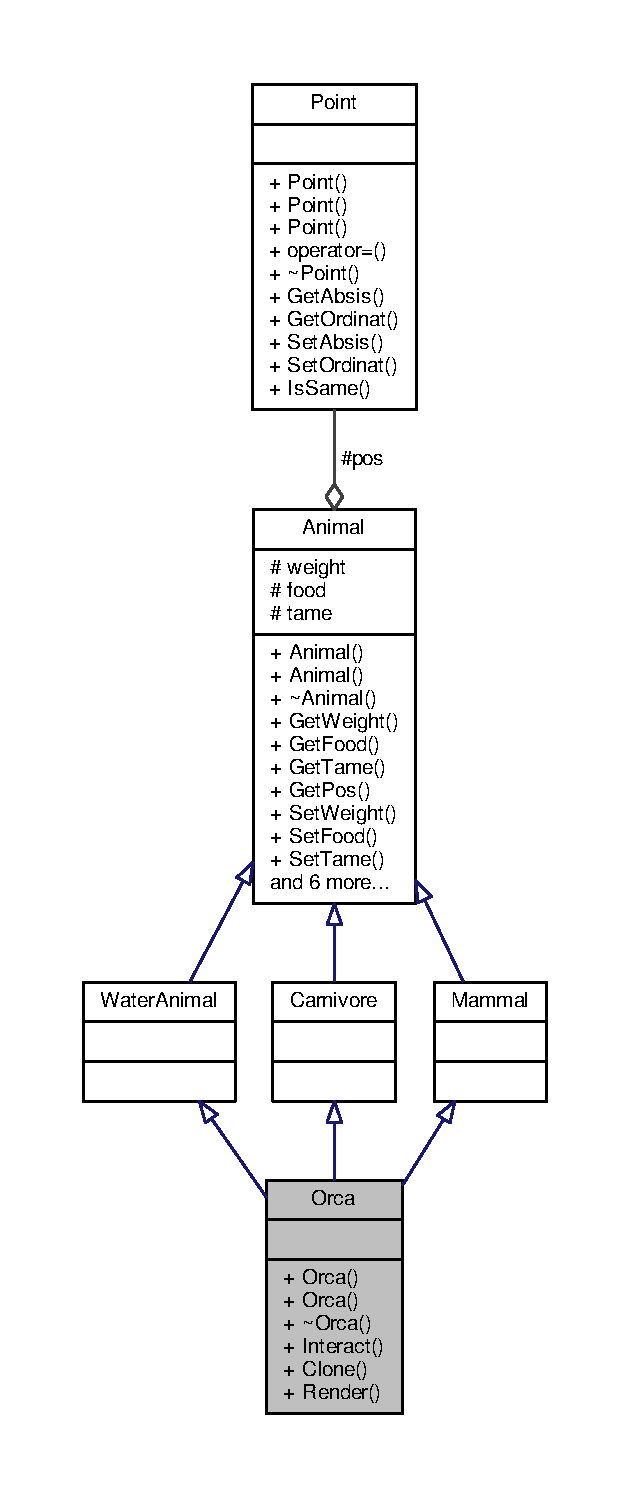
\includegraphics[height=550pt]{classOrca__coll__graph}
\end{center}
\end{figure}
\subsection*{Public Member Functions}
\begin{DoxyCompactItemize}
\item 
\hyperlink{classOrca_a1efb2589b67f95863f7c8a653cfb13f3}{Orca} ()
\begin{DoxyCompactList}\small\item\em Constructor. Menciptakan objek \hyperlink{classOrca}{Orca}. \end{DoxyCompactList}\item 
virtual \hyperlink{classOrca_a964d6cd8b816cfa70f5194457b9382c0}{$\sim$\+Orca} ()
\begin{DoxyCompactList}\small\item\em Destructor. \end{DoxyCompactList}\item 
string \hyperlink{classOrca_adf95ca04578ac04aaa717ef2dd11bf4c}{Interact} ()
\begin{DoxyCompactList}\small\item\em Interaksi yang dilakukan \hyperlink{classOrca}{Orca}. \end{DoxyCompactList}\item 
virtual \hyperlink{classOrca}{Orca} $\ast$ \hyperlink{classOrca_ac44eb30486ba4051eefa914dc8cd670f}{Clone} () const 
\begin{DoxyCompactList}\small\item\em Melakukan cloning untuk menciptakan objek \hyperlink{classOrca}{Orca} baru. \end{DoxyCompactList}\item 
char \hyperlink{classOrca_a0673bfc8e70af67b463a4fcae224d9d5}{Render} ()
\begin{DoxyCompactList}\small\item\em Render dari \hyperlink{classOrca}{Orca}. \end{DoxyCompactList}\end{DoxyCompactItemize}
\subsection*{Additional Inherited Members}


\subsection{Detailed Description}
Kelas \hyperlink{classOrca}{Orca} merupakan kelas untuk real object \hyperlink{classOrca}{Orca} 

\subsection{Constructor \& Destructor Documentation}
\index{Orca@{Orca}!Orca@{Orca}}
\index{Orca@{Orca}!Orca@{Orca}}
\subsubsection[{\texorpdfstring{Orca()}{Orca()}}]{\setlength{\rightskip}{0pt plus 5cm}Orca\+::\+Orca (
\begin{DoxyParamCaption}
{}
\end{DoxyParamCaption}
)\hspace{0.3cm}{\ttfamily [inline]}}\hypertarget{classOrca_a1efb2589b67f95863f7c8a653cfb13f3}{}\label{classOrca_a1efb2589b67f95863f7c8a653cfb13f3}


Constructor. Menciptakan objek \hyperlink{classOrca}{Orca}. 

\index{Orca@{Orca}!````~Orca@{$\sim$\+Orca}}
\index{````~Orca@{$\sim$\+Orca}!Orca@{Orca}}
\subsubsection[{\texorpdfstring{$\sim$\+Orca()}{~Orca()}}]{\setlength{\rightskip}{0pt plus 5cm}virtual Orca\+::$\sim$\+Orca (
\begin{DoxyParamCaption}
{}
\end{DoxyParamCaption}
)\hspace{0.3cm}{\ttfamily [inline]}, {\ttfamily [virtual]}}\hypertarget{classOrca_a964d6cd8b816cfa70f5194457b9382c0}{}\label{classOrca_a964d6cd8b816cfa70f5194457b9382c0}


Destructor. 



\subsection{Member Function Documentation}
\index{Orca@{Orca}!Clone@{Clone}}
\index{Clone@{Clone}!Orca@{Orca}}
\subsubsection[{\texorpdfstring{Clone() const }{Clone() const }}]{\setlength{\rightskip}{0pt plus 5cm}virtual {\bf Orca}$\ast$ Orca\+::\+Clone (
\begin{DoxyParamCaption}
{}
\end{DoxyParamCaption}
) const\hspace{0.3cm}{\ttfamily [inline]}, {\ttfamily [virtual]}}\hypertarget{classOrca_ac44eb30486ba4051eefa914dc8cd670f}{}\label{classOrca_ac44eb30486ba4051eefa914dc8cd670f}


Melakukan cloning untuk menciptakan objek \hyperlink{classOrca}{Orca} baru. 

\begin{DoxyReturn}{Returns}
Mengembalikan pointer to \hyperlink{classOrca}{Orca} objek tersebut. 
\end{DoxyReturn}


Implements \hyperlink{classAnimal_a3fc95e2a588b653b9b315e6c7a29c89f}{Animal}.

\index{Orca@{Orca}!Interact@{Interact}}
\index{Interact@{Interact}!Orca@{Orca}}
\subsubsection[{\texorpdfstring{Interact()}{Interact()}}]{\setlength{\rightskip}{0pt plus 5cm}string Orca\+::\+Interact (
\begin{DoxyParamCaption}
{}
\end{DoxyParamCaption}
)\hspace{0.3cm}{\ttfamily [inline]}, {\ttfamily [virtual]}}\hypertarget{classOrca_adf95ca04578ac04aaa717ef2dd11bf4c}{}\label{classOrca_adf95ca04578ac04aaa717ef2dd11bf4c}


Interaksi yang dilakukan \hyperlink{classOrca}{Orca}. 

\begin{DoxyReturn}{Returns}
Mengembalikan string yang merepresentasikan suara \hyperlink{classOrca}{Orca}. 
\end{DoxyReturn}


Implements \hyperlink{classAnimal_ad5a55fb0355a9425fee6611003d9892c}{Animal}.

\index{Orca@{Orca}!Render@{Render}}
\index{Render@{Render}!Orca@{Orca}}
\subsubsection[{\texorpdfstring{Render()}{Render()}}]{\setlength{\rightskip}{0pt plus 5cm}char Orca\+::\+Render (
\begin{DoxyParamCaption}
{}
\end{DoxyParamCaption}
)\hspace{0.3cm}{\ttfamily [inline]}, {\ttfamily [virtual]}}\hypertarget{classOrca_a0673bfc8e70af67b463a4fcae224d9d5}{}\label{classOrca_a0673bfc8e70af67b463a4fcae224d9d5}


Render dari \hyperlink{classOrca}{Orca}. 

\begin{DoxyReturn}{Returns}
Mengembalikan char yang merupakan representasi kode \hyperlink{classOrca}{Orca}. 
\end{DoxyReturn}


Implements \hyperlink{classAnimal_a43a47c0f41d211128e04abc6add53def}{Animal}.



The documentation for this class was generated from the following file\+:\begin{DoxyCompactItemize}
\item 
orca/\hyperlink{orca_8h}{orca.\+h}\end{DoxyCompactItemize}

\hypertarget{classOwl}{}\section{Owl Class Reference}
\label{classOwl}\index{Owl@{Owl}}


{\ttfamily \#include $<$owl.\+h$>$}



Inheritance diagram for Owl\+:
\nopagebreak
\begin{figure}[H]
\begin{center}
\leavevmode
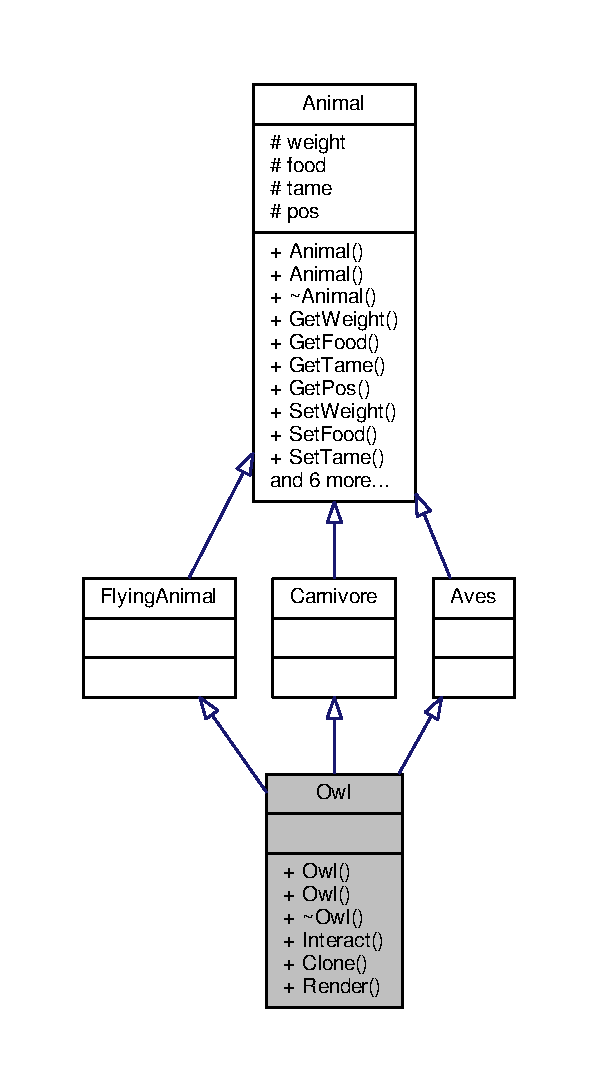
\includegraphics[width=210pt]{classOwl__inherit__graph}
\end{center}
\end{figure}


Collaboration diagram for Owl\+:
\nopagebreak
\begin{figure}[H]
\begin{center}
\leavevmode
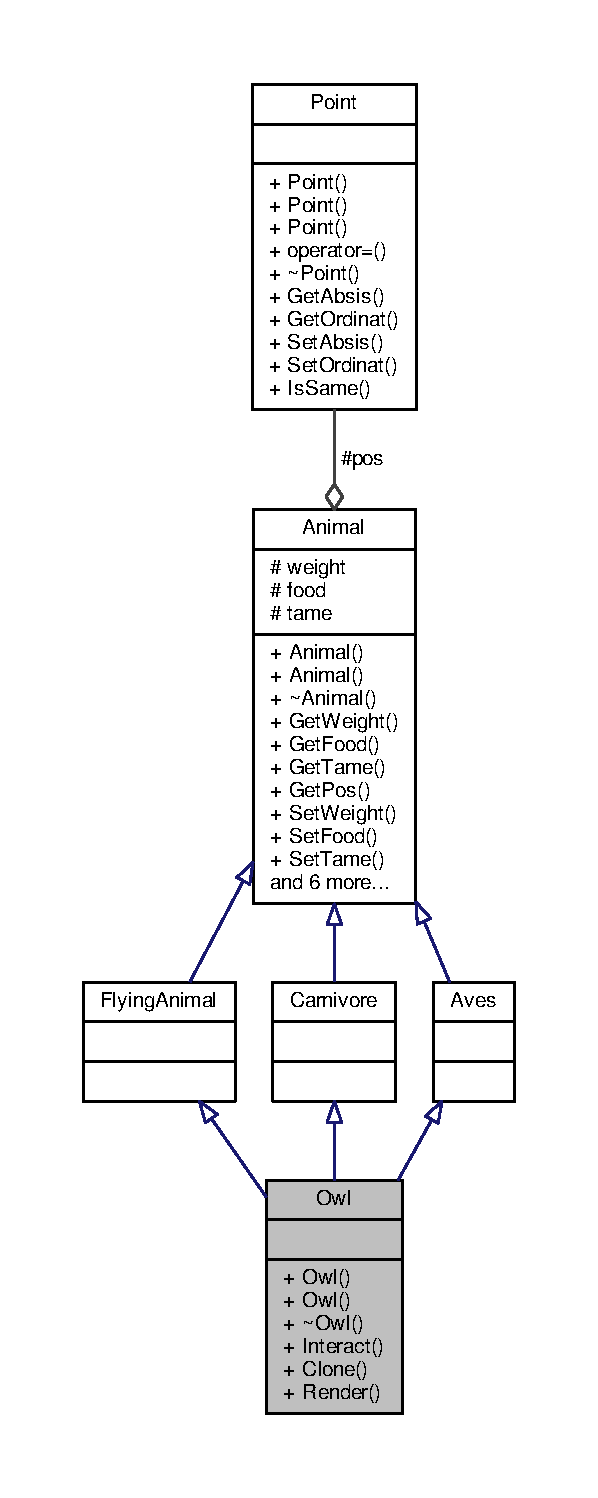
\includegraphics[height=550pt]{classOwl__coll__graph}
\end{center}
\end{figure}
\subsection*{Public Member Functions}
\begin{DoxyCompactItemize}
\item 
\hyperlink{classOwl_a0a5c549eb9ac3099f04dbcea78c79f6a}{Owl} ()
\begin{DoxyCompactList}\small\item\em Constructor. Menciptakan objek \hyperlink{classOwl}{Owl}. \end{DoxyCompactList}\item 
virtual \hyperlink{classOwl_af8238b610fbfd53c4d3153fb2d993ab7}{$\sim$\+Owl} ()
\begin{DoxyCompactList}\small\item\em Destructor. \end{DoxyCompactList}\item 
string \hyperlink{classOwl_ac3c735f8a34b46780a0efd052319e7f3}{Interact} ()
\begin{DoxyCompactList}\small\item\em Interaksi yang dilakukan \hyperlink{classOwl}{Owl}. \end{DoxyCompactList}\item 
virtual \hyperlink{classOwl}{Owl} $\ast$ \hyperlink{classOwl_a585e73d53d76b2db489613b7f0b6eecc}{Clone} () const 
\begin{DoxyCompactList}\small\item\em Melakukan cloning untuk menciptakan objek \hyperlink{classOwl}{Owl} baru. \end{DoxyCompactList}\item 
char \hyperlink{classOwl_ab4ecc1fc8da822f97299709508f7806d}{Render} ()
\begin{DoxyCompactList}\small\item\em Render dari \hyperlink{classOwl}{Owl}. \end{DoxyCompactList}\end{DoxyCompactItemize}
\subsection*{Additional Inherited Members}


\subsection{Detailed Description}
Kelas \hyperlink{classOwl}{Owl} merupakan kelas untuk real object \hyperlink{classOwl}{Owl} 

\subsection{Constructor \& Destructor Documentation}
\index{Owl@{Owl}!Owl@{Owl}}
\index{Owl@{Owl}!Owl@{Owl}}
\subsubsection[{\texorpdfstring{Owl()}{Owl()}}]{\setlength{\rightskip}{0pt plus 5cm}Owl\+::\+Owl (
\begin{DoxyParamCaption}
{}
\end{DoxyParamCaption}
)\hspace{0.3cm}{\ttfamily [inline]}}\hypertarget{classOwl_a0a5c549eb9ac3099f04dbcea78c79f6a}{}\label{classOwl_a0a5c549eb9ac3099f04dbcea78c79f6a}


Constructor. Menciptakan objek \hyperlink{classOwl}{Owl}. 

\index{Owl@{Owl}!````~Owl@{$\sim$\+Owl}}
\index{````~Owl@{$\sim$\+Owl}!Owl@{Owl}}
\subsubsection[{\texorpdfstring{$\sim$\+Owl()}{~Owl()}}]{\setlength{\rightskip}{0pt plus 5cm}virtual Owl\+::$\sim$\+Owl (
\begin{DoxyParamCaption}
{}
\end{DoxyParamCaption}
)\hspace{0.3cm}{\ttfamily [inline]}, {\ttfamily [virtual]}}\hypertarget{classOwl_af8238b610fbfd53c4d3153fb2d993ab7}{}\label{classOwl_af8238b610fbfd53c4d3153fb2d993ab7}


Destructor. 



\subsection{Member Function Documentation}
\index{Owl@{Owl}!Clone@{Clone}}
\index{Clone@{Clone}!Owl@{Owl}}
\subsubsection[{\texorpdfstring{Clone() const }{Clone() const }}]{\setlength{\rightskip}{0pt plus 5cm}virtual {\bf Owl}$\ast$ Owl\+::\+Clone (
\begin{DoxyParamCaption}
{}
\end{DoxyParamCaption}
) const\hspace{0.3cm}{\ttfamily [inline]}, {\ttfamily [virtual]}}\hypertarget{classOwl_a585e73d53d76b2db489613b7f0b6eecc}{}\label{classOwl_a585e73d53d76b2db489613b7f0b6eecc}


Melakukan cloning untuk menciptakan objek \hyperlink{classOwl}{Owl} baru. 

\begin{DoxyReturn}{Returns}
Mengembalikan pointer to \hyperlink{classOwl}{Owl} objek tersebut. 
\end{DoxyReturn}


Implements \hyperlink{classAnimal_a3fc95e2a588b653b9b315e6c7a29c89f}{Animal}.

\index{Owl@{Owl}!Interact@{Interact}}
\index{Interact@{Interact}!Owl@{Owl}}
\subsubsection[{\texorpdfstring{Interact()}{Interact()}}]{\setlength{\rightskip}{0pt plus 5cm}string Owl\+::\+Interact (
\begin{DoxyParamCaption}
{}
\end{DoxyParamCaption}
)\hspace{0.3cm}{\ttfamily [inline]}, {\ttfamily [virtual]}}\hypertarget{classOwl_ac3c735f8a34b46780a0efd052319e7f3}{}\label{classOwl_ac3c735f8a34b46780a0efd052319e7f3}


Interaksi yang dilakukan \hyperlink{classOwl}{Owl}. 

\begin{DoxyReturn}{Returns}
Mengembalikan string yang merepresentasikan suara \hyperlink{classOwl}{Owl}. 
\end{DoxyReturn}


Implements \hyperlink{classAnimal_ad5a55fb0355a9425fee6611003d9892c}{Animal}.

\index{Owl@{Owl}!Render@{Render}}
\index{Render@{Render}!Owl@{Owl}}
\subsubsection[{\texorpdfstring{Render()}{Render()}}]{\setlength{\rightskip}{0pt plus 5cm}char Owl\+::\+Render (
\begin{DoxyParamCaption}
{}
\end{DoxyParamCaption}
)\hspace{0.3cm}{\ttfamily [inline]}, {\ttfamily [virtual]}}\hypertarget{classOwl_ab4ecc1fc8da822f97299709508f7806d}{}\label{classOwl_ab4ecc1fc8da822f97299709508f7806d}


Render dari \hyperlink{classOwl}{Owl}. 

\begin{DoxyReturn}{Returns}
Mengembalikan char yang merupakan representasi kode \hyperlink{classOwl}{Owl}. 
\end{DoxyReturn}


Implements \hyperlink{classAnimal_a43a47c0f41d211128e04abc6add53def}{Animal}.



The documentation for this class was generated from the following file\+:\begin{DoxyCompactItemize}
\item 
owl/\hyperlink{owl_8h}{owl.\+h}\end{DoxyCompactItemize}

\hypertarget{classPark}{}\section{Park Class Reference}
\label{classPark}\index{Park@{Park}}


{\ttfamily \#include $<$park.\+h$>$}



Inheritance diagram for Park\+:
\nopagebreak
\begin{figure}[H]
\begin{center}
\leavevmode
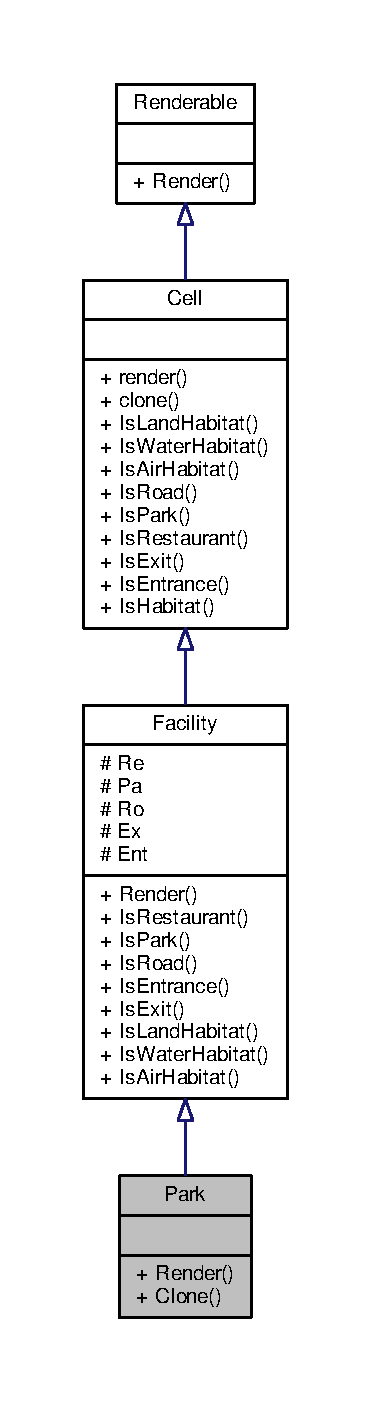
\includegraphics[height=550pt]{classPark__inherit__graph}
\end{center}
\end{figure}


Collaboration diagram for Park\+:
\nopagebreak
\begin{figure}[H]
\begin{center}
\leavevmode
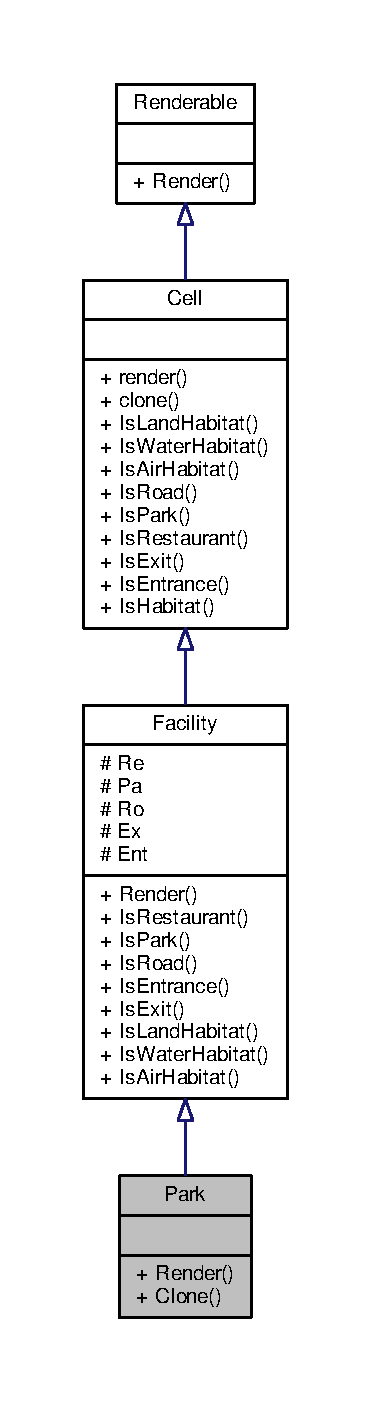
\includegraphics[height=550pt]{classPark__coll__graph}
\end{center}
\end{figure}
\subsection*{Public Member Functions}
\begin{DoxyCompactItemize}
\item 
char \hyperlink{classPark_a98b2a346d5ec6703b2e988588950947e}{Render} ()
\begin{DoxyCompactList}\small\item\em Render dari \hyperlink{classPark}{Park}. \end{DoxyCompactList}\item 
virtual \hyperlink{classPark}{Park} $\ast$ \hyperlink{classPark_a573db7d7f393802c02c753572c33bef4}{Clone} () const 
\begin{DoxyCompactList}\small\item\em Melakukan cloning untuk menciptakan objek \hyperlink{classPark}{Park} baru. \end{DoxyCompactList}\end{DoxyCompactItemize}
\subsection*{Additional Inherited Members}


\subsection{Detailed Description}
Kelas \hyperlink{classPark}{Park} merepresentasikan fasilitas taman 

\subsection{Member Function Documentation}
\index{Park@{Park}!Clone@{Clone}}
\index{Clone@{Clone}!Park@{Park}}
\subsubsection[{\texorpdfstring{Clone() const }{Clone() const }}]{\setlength{\rightskip}{0pt plus 5cm}virtual {\bf Park}$\ast$ Park\+::\+Clone (
\begin{DoxyParamCaption}
{}
\end{DoxyParamCaption}
) const\hspace{0.3cm}{\ttfamily [inline]}, {\ttfamily [virtual]}}\hypertarget{classPark_a573db7d7f393802c02c753572c33bef4}{}\label{classPark_a573db7d7f393802c02c753572c33bef4}


Melakukan cloning untuk menciptakan objek \hyperlink{classPark}{Park} baru. 

\begin{DoxyReturn}{Returns}
Mengembalikan pointer to \hyperlink{classPark}{Park} objek tersebut. 
\end{DoxyReturn}
\index{Park@{Park}!Render@{Render}}
\index{Render@{Render}!Park@{Park}}
\subsubsection[{\texorpdfstring{Render()}{Render()}}]{\setlength{\rightskip}{0pt plus 5cm}char Park\+::\+Render (
\begin{DoxyParamCaption}
{}
\end{DoxyParamCaption}
)\hspace{0.3cm}{\ttfamily [inline]}, {\ttfamily [virtual]}}\hypertarget{classPark_a98b2a346d5ec6703b2e988588950947e}{}\label{classPark_a98b2a346d5ec6703b2e988588950947e}


Render dari \hyperlink{classPark}{Park}. 

\begin{DoxyReturn}{Returns}
Mengembalikan char yang merupakan representasi kode \hyperlink{classPark}{Park}. 
\end{DoxyReturn}


Implements \hyperlink{classFacility_a177b3f9cd142fe4521c1d15b00d3675c}{Facility}.



The documentation for this class was generated from the following file\+:\begin{DoxyCompactItemize}
\item 
\hyperlink{park_8h}{park.\+h}\end{DoxyCompactItemize}

\hypertarget{classParrot}{}\section{Parrot Class Reference}
\label{classParrot}\index{Parrot@{Parrot}}


{\ttfamily \#include $<$parrot.\+h$>$}



Inheritance diagram for Parrot\+:
% FIG 0


Collaboration diagram for Parrot\+:
% FIG 1
\subsection*{Public Member Functions}
\begin{DoxyCompactItemize}
\item 
\hyperlink{classParrot_adfd08f638064b09dc46924ded14d1b32}{Parrot} ()
\begin{DoxyCompactList}\small\item\em Constructor. Menciptakan objek \hyperlink{classParrot}{Parrot}. \end{DoxyCompactList}\item 
\hyperlink{classParrot_a98ad57fac6ea488daf92b33c2d8ae57f}{Parrot} (float w, float f, bool t)
\begin{DoxyCompactList}\small\item\em Constructor dengan parameter. Menciptakan objek \hyperlink{classParrot}{Parrot} dengan berat w, jumlah makanan f, dan status jinak t. \end{DoxyCompactList}\item 
virtual \hyperlink{classParrot_a02300897ced64c5a28347d385f4f0f00}{$\sim$\+Parrot} ()
\begin{DoxyCompactList}\small\item\em Destructor. \end{DoxyCompactList}\item 
string \hyperlink{classParrot_a3fdf1aa0851d53d31b5d225d755e4995}{Interact} ()
\begin{DoxyCompactList}\small\item\em Interaksi yang dilakukan \hyperlink{classParrot}{Parrot}. \end{DoxyCompactList}\item 
virtual \hyperlink{classParrot}{Parrot} $\ast$ \hyperlink{classParrot_aec7fd1385827d67522e1baf3242078b0}{Clone} () const 
\begin{DoxyCompactList}\small\item\em Melakukan cloning untuk menciptakan objek \hyperlink{classParrot}{Parrot} baru. \end{DoxyCompactList}\item 
char \hyperlink{classParrot_a27c491ab4ae56491fbe8d74e494bc46d}{Render} ()
\begin{DoxyCompactList}\small\item\em Render dari \hyperlink{classParrot}{Parrot}. \end{DoxyCompactList}\end{DoxyCompactItemize}
\subsection*{Additional Inherited Members}


\subsection{Detailed Description}
kelas \hyperlink{classParrot}{Parrot} merupakan kelas untuk real object \hyperlink{classParrot}{Parrot} 

\subsection{Constructor \& Destructor Documentation}
\index{Parrot@{Parrot}!Parrot@{Parrot}}
\index{Parrot@{Parrot}!Parrot@{Parrot}}
\subsubsection[{\texorpdfstring{Parrot()}{Parrot()}}]{\setlength{\rightskip}{0pt plus 5cm}Parrot\+::\+Parrot (
\begin{DoxyParamCaption}
{}
\end{DoxyParamCaption}
)\hspace{0.3cm}{\ttfamily [inline]}}\hypertarget{classParrot_adfd08f638064b09dc46924ded14d1b32}{}\label{classParrot_adfd08f638064b09dc46924ded14d1b32}


Constructor. Menciptakan objek \hyperlink{classParrot}{Parrot}. 

\index{Parrot@{Parrot}!Parrot@{Parrot}}
\index{Parrot@{Parrot}!Parrot@{Parrot}}
\subsubsection[{\texorpdfstring{Parrot(float w, float f, bool t)}{Parrot(float w, float f, bool t)}}]{\setlength{\rightskip}{0pt plus 5cm}Parrot\+::\+Parrot (
\begin{DoxyParamCaption}
\item[{float}]{w, }
\item[{float}]{f, }
\item[{bool}]{t}
\end{DoxyParamCaption}
)\hspace{0.3cm}{\ttfamily [inline]}}\hypertarget{classParrot_a98ad57fac6ea488daf92b33c2d8ae57f}{}\label{classParrot_a98ad57fac6ea488daf92b33c2d8ae57f}


Constructor dengan parameter. Menciptakan objek \hyperlink{classParrot}{Parrot} dengan berat w, jumlah makanan f, dan status jinak t. 


\begin{DoxyParams}{Parameters}
{\em w} & Berat \hyperlink{classParrot}{Parrot}. \\
\hline
{\em f} & Jumlah makanan \hyperlink{classParrot}{Parrot}. \\
\hline
{\em t} & Status jinak \hyperlink{classParrot}{Parrot}. \\
\hline
\end{DoxyParams}
\index{Parrot@{Parrot}!````~Parrot@{$\sim$\+Parrot}}
\index{````~Parrot@{$\sim$\+Parrot}!Parrot@{Parrot}}
\subsubsection[{\texorpdfstring{$\sim$\+Parrot()}{~Parrot()}}]{\setlength{\rightskip}{0pt plus 5cm}virtual Parrot\+::$\sim$\+Parrot (
\begin{DoxyParamCaption}
{}
\end{DoxyParamCaption}
)\hspace{0.3cm}{\ttfamily [inline]}, {\ttfamily [virtual]}}\hypertarget{classParrot_a02300897ced64c5a28347d385f4f0f00}{}\label{classParrot_a02300897ced64c5a28347d385f4f0f00}


Destructor. 



\subsection{Member Function Documentation}
\index{Parrot@{Parrot}!Clone@{Clone}}
\index{Clone@{Clone}!Parrot@{Parrot}}
\subsubsection[{\texorpdfstring{Clone() const }{Clone() const }}]{\setlength{\rightskip}{0pt plus 5cm}virtual {\bf Parrot}$\ast$ Parrot\+::\+Clone (
\begin{DoxyParamCaption}
{}
\end{DoxyParamCaption}
) const\hspace{0.3cm}{\ttfamily [inline]}, {\ttfamily [virtual]}}\hypertarget{classParrot_aec7fd1385827d67522e1baf3242078b0}{}\label{classParrot_aec7fd1385827d67522e1baf3242078b0}


Melakukan cloning untuk menciptakan objek \hyperlink{classParrot}{Parrot} baru. 

\begin{DoxyReturn}{Returns}
Mengembalikan pointer to \hyperlink{classParrot}{Parrot} objek tersebut. 
\end{DoxyReturn}


Implements \hyperlink{classAnimal_a3fc95e2a588b653b9b315e6c7a29c89f}{Animal}.

\index{Parrot@{Parrot}!Interact@{Interact}}
\index{Interact@{Interact}!Parrot@{Parrot}}
\subsubsection[{\texorpdfstring{Interact()}{Interact()}}]{\setlength{\rightskip}{0pt plus 5cm}string Parrot\+::\+Interact (
\begin{DoxyParamCaption}
{}
\end{DoxyParamCaption}
)\hspace{0.3cm}{\ttfamily [inline]}, {\ttfamily [virtual]}}\hypertarget{classParrot_a3fdf1aa0851d53d31b5d225d755e4995}{}\label{classParrot_a3fdf1aa0851d53d31b5d225d755e4995}


Interaksi yang dilakukan \hyperlink{classParrot}{Parrot}. 

\begin{DoxyReturn}{Returns}
Mengembalikan string yang merepresentasikan suara \hyperlink{classParrot}{Parrot}. 
\end{DoxyReturn}


Implements \hyperlink{classAnimal_ad5a55fb0355a9425fee6611003d9892c}{Animal}.

\index{Parrot@{Parrot}!Render@{Render}}
\index{Render@{Render}!Parrot@{Parrot}}
\subsubsection[{\texorpdfstring{Render()}{Render()}}]{\setlength{\rightskip}{0pt plus 5cm}char Parrot\+::\+Render (
\begin{DoxyParamCaption}
{}
\end{DoxyParamCaption}
)\hspace{0.3cm}{\ttfamily [inline]}, {\ttfamily [virtual]}}\hypertarget{classParrot_a27c491ab4ae56491fbe8d74e494bc46d}{}\label{classParrot_a27c491ab4ae56491fbe8d74e494bc46d}


Render dari \hyperlink{classParrot}{Parrot}. 

\begin{DoxyReturn}{Returns}
Mengembalikan char yang merupakan representasi kode \hyperlink{classParrot}{Parrot}. 
\end{DoxyReturn}


Implements \hyperlink{classAnimal_a43a47c0f41d211128e04abc6add53def}{Animal}.



The documentation for this class was generated from the following file\+:\begin{DoxyCompactItemize}
\item 
parrot/\hyperlink{parrot_8h}{parrot.\+h}\end{DoxyCompactItemize}

\hypertarget{classPisces}{}\section{Pisces Class Reference}
\label{classPisces}\index{Pisces@{Pisces}}


{\ttfamily \#include $<$pisces.\+h$>$}



Inheritance diagram for Pisces\+:
\nopagebreak
\begin{figure}[H]
\begin{center}
\leavevmode
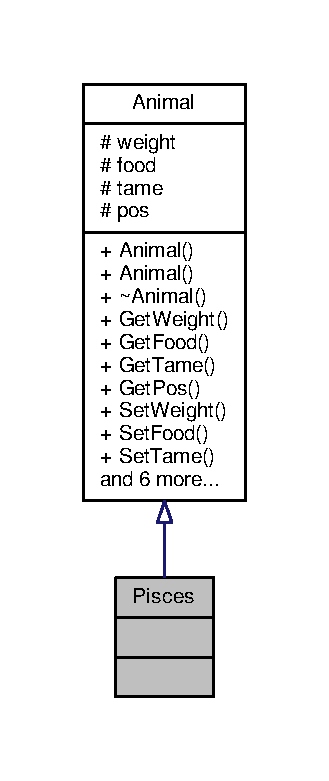
\includegraphics[width=158pt]{classPisces__inherit__graph}
\end{center}
\end{figure}


Collaboration diagram for Pisces\+:
\nopagebreak
\begin{figure}[H]
\begin{center}
\leavevmode
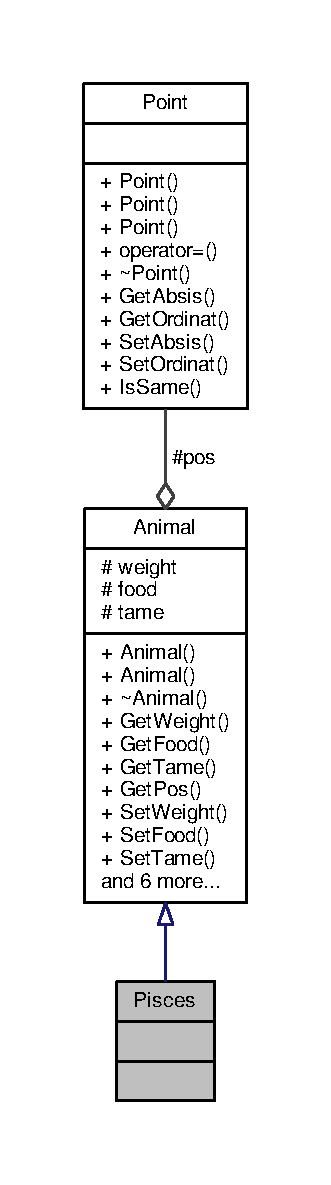
\includegraphics[height=550pt]{classPisces__coll__graph}
\end{center}
\end{figure}
\subsection*{Additional Inherited Members}


\subsection{Detailed Description}
Kelas abstrak \hyperlink{classPisces}{Pisces} 

The documentation for this class was generated from the following file\+:\begin{DoxyCompactItemize}
\item 
\hyperlink{pisces_8h}{pisces.\+h}\end{DoxyCompactItemize}

\hypertarget{classPoint}{}\section{Point Class Reference}
\label{classPoint}\index{Point@{Point}}


{\ttfamily \#include $<$point.\+h$>$}



Collaboration diagram for Point\+:
\nopagebreak
\begin{figure}[H]
\begin{center}
\leavevmode
\includegraphics[width=159pt]{classPoint__coll__graph}
\end{center}
\end{figure}
\subsection*{Public Member Functions}
\begin{DoxyCompactItemize}
\item 
\hyperlink{classPoint_ad92f2337b839a94ce97dcdb439b4325a}{Point} ()
\begin{DoxyCompactList}\small\item\em Constructor. Menciptakan point kosong dengan absis dan ordinat sama dengan 0. \end{DoxyCompactList}\item 
\hyperlink{classPoint_a3634e1e4d94c1268ddaca3909f23b39b}{Point} (int abs, int ord)
\begin{DoxyCompactList}\small\item\em Constructor dengan parameter. Menciptakan point kosong dengan absis abs dan ordinat ord. \end{DoxyCompactList}\item 
\hyperlink{classPoint_a7e32c5a7f878c49ed9f1777b622cc06c}{Point} (const \hyperlink{classPoint}{Point} \&P)
\begin{DoxyCompactList}\small\item\em Copy Constructor. \end{DoxyCompactList}\item 
\hyperlink{classPoint}{Point} \& \hyperlink{classPoint_a24f658e4631df755120d856de77e3cbb}{operator=} (const \hyperlink{classPoint}{Point} \&P)
\begin{DoxyCompactList}\small\item\em Operator =. \end{DoxyCompactList}\item 
\hyperlink{classPoint_a395fa04b4ec126b66fc053f829a30cc1}{$\sim$\+Point} ()
\begin{DoxyCompactList}\small\item\em Destructor. \end{DoxyCompactList}\item 
int \hyperlink{classPoint_af9d064339ffb2f87abb6574dbfc9cdb2}{Get\+Absis} () const 
\begin{DoxyCompactList}\small\item\em Getter absis. \end{DoxyCompactList}\item 
int \hyperlink{classPoint_ace648a3faea60f8102d645d4b5a40b1a}{Get\+Ordinat} () const 
\begin{DoxyCompactList}\small\item\em Getter ordinat. \end{DoxyCompactList}\item 
void \hyperlink{classPoint_a0ba1dc33923b3aaa7678a07ffa022b06}{Set\+Absis} (int abs)
\begin{DoxyCompactList}\small\item\em Setter absis. \end{DoxyCompactList}\item 
void \hyperlink{classPoint_ae672d4952c6c730d104588a67304aed1}{Set\+Ordinat} (int ord)
\begin{DoxyCompactList}\small\item\em Setter ordinat. \end{DoxyCompactList}\item 
bool \hyperlink{classPoint_a19e146331c9acef35c6941bee733925e}{Is\+Same} (\hyperlink{classPoint}{Point} P) const 
\begin{DoxyCompactList}\small\item\em Memeriksa kesamaan dua point. \end{DoxyCompactList}\end{DoxyCompactItemize}


\subsection{Detailed Description}
Kelas \hyperlink{classPoint}{Point} merupakan kelas dengan atribut absis dan ordinat 

\subsection{Constructor \& Destructor Documentation}
\index{Point@{Point}!Point@{Point}}
\index{Point@{Point}!Point@{Point}}
\subsubsection[{\texorpdfstring{Point()}{Point()}}]{\setlength{\rightskip}{0pt plus 5cm}Point\+::\+Point (
\begin{DoxyParamCaption}
{}
\end{DoxyParamCaption}
)}\hypertarget{classPoint_ad92f2337b839a94ce97dcdb439b4325a}{}\label{classPoint_ad92f2337b839a94ce97dcdb439b4325a}


Constructor. Menciptakan point kosong dengan absis dan ordinat sama dengan 0. 

\index{Point@{Point}!Point@{Point}}
\index{Point@{Point}!Point@{Point}}
\subsubsection[{\texorpdfstring{Point(int abs, int ord)}{Point(int abs, int ord)}}]{\setlength{\rightskip}{0pt plus 5cm}Point\+::\+Point (
\begin{DoxyParamCaption}
\item[{int}]{abs, }
\item[{int}]{ord}
\end{DoxyParamCaption}
)}\hypertarget{classPoint_a3634e1e4d94c1268ddaca3909f23b39b}{}\label{classPoint_a3634e1e4d94c1268ddaca3909f23b39b}


Constructor dengan parameter. Menciptakan point kosong dengan absis abs dan ordinat ord. 


\begin{DoxyParams}{Parameters}
{\em abs} & Nilai absis point. \\
\hline
{\em ord} & Nilai ordinat point. \\
\hline
\end{DoxyParams}
\index{Point@{Point}!Point@{Point}}
\index{Point@{Point}!Point@{Point}}
\subsubsection[{\texorpdfstring{Point(const Point \&\+P)}{Point(const Point &P)}}]{\setlength{\rightskip}{0pt plus 5cm}Point\+::\+Point (
\begin{DoxyParamCaption}
\item[{const {\bf Point} \&}]{P}
\end{DoxyParamCaption}
)}\hypertarget{classPoint_a7e32c5a7f878c49ed9f1777b622cc06c}{}\label{classPoint_a7e32c5a7f878c49ed9f1777b622cc06c}


Copy Constructor. 


\begin{DoxyParams}{Parameters}
{\em P} & Objek yang akan di-\/copy. \\
\hline
\end{DoxyParams}
\index{Point@{Point}!````~Point@{$\sim$\+Point}}
\index{````~Point@{$\sim$\+Point}!Point@{Point}}
\subsubsection[{\texorpdfstring{$\sim$\+Point()}{~Point()}}]{\setlength{\rightskip}{0pt plus 5cm}Point\+::$\sim$\+Point (
\begin{DoxyParamCaption}
{}
\end{DoxyParamCaption}
)\hspace{0.3cm}{\ttfamily [inline]}}\hypertarget{classPoint_a395fa04b4ec126b66fc053f829a30cc1}{}\label{classPoint_a395fa04b4ec126b66fc053f829a30cc1}


Destructor. 



\subsection{Member Function Documentation}
\index{Point@{Point}!Get\+Absis@{Get\+Absis}}
\index{Get\+Absis@{Get\+Absis}!Point@{Point}}
\subsubsection[{\texorpdfstring{Get\+Absis() const }{GetAbsis() const }}]{\setlength{\rightskip}{0pt plus 5cm}int Point\+::\+Get\+Absis (
\begin{DoxyParamCaption}
{}
\end{DoxyParamCaption}
) const}\hypertarget{classPoint_af9d064339ffb2f87abb6574dbfc9cdb2}{}\label{classPoint_af9d064339ffb2f87abb6574dbfc9cdb2}


Getter absis. 

\begin{DoxyReturn}{Returns}
Mengembalikan nilai absis point. 
\end{DoxyReturn}
\index{Point@{Point}!Get\+Ordinat@{Get\+Ordinat}}
\index{Get\+Ordinat@{Get\+Ordinat}!Point@{Point}}
\subsubsection[{\texorpdfstring{Get\+Ordinat() const }{GetOrdinat() const }}]{\setlength{\rightskip}{0pt plus 5cm}int Point\+::\+Get\+Ordinat (
\begin{DoxyParamCaption}
{}
\end{DoxyParamCaption}
) const}\hypertarget{classPoint_ace648a3faea60f8102d645d4b5a40b1a}{}\label{classPoint_ace648a3faea60f8102d645d4b5a40b1a}


Getter ordinat. 

\begin{DoxyReturn}{Returns}
Mengembalikan nilai ordinat point. 
\end{DoxyReturn}
\index{Point@{Point}!Is\+Same@{Is\+Same}}
\index{Is\+Same@{Is\+Same}!Point@{Point}}
\subsubsection[{\texorpdfstring{Is\+Same(\+Point P) const }{IsSame(Point P) const }}]{\setlength{\rightskip}{0pt plus 5cm}bool Point\+::\+Is\+Same (
\begin{DoxyParamCaption}
\item[{{\bf Point}}]{P}
\end{DoxyParamCaption}
) const}\hypertarget{classPoint_a19e146331c9acef35c6941bee733925e}{}\label{classPoint_a19e146331c9acef35c6941bee733925e}


Memeriksa kesamaan dua point. 


\begin{DoxyParams}{Parameters}
{\em P} & Objek yang akan dibandingkan. \\
\hline
\end{DoxyParams}
\begin{DoxyReturn}{Returns}
Menghasilkan true jika P memiliki nilai yang sama dengan current object. 
\end{DoxyReturn}
\index{Point@{Point}!operator=@{operator=}}
\index{operator=@{operator=}!Point@{Point}}
\subsubsection[{\texorpdfstring{operator=(const Point \&\+P)}{operator=(const Point &P)}}]{\setlength{\rightskip}{0pt plus 5cm}{\bf Point} \& Point\+::operator= (
\begin{DoxyParamCaption}
\item[{const {\bf Point} \&}]{P}
\end{DoxyParamCaption}
)}\hypertarget{classPoint_a24f658e4631df755120d856de77e3cbb}{}\label{classPoint_a24f658e4631df755120d856de77e3cbb}


Operator =. 


\begin{DoxyParams}{Parameters}
{\em P} & Objek yang akan diassign. \\
\hline
\end{DoxyParams}
\begin{DoxyReturn}{Returns}
Menghasilkan objek hasil copy objek P. 
\end{DoxyReturn}
\index{Point@{Point}!Set\+Absis@{Set\+Absis}}
\index{Set\+Absis@{Set\+Absis}!Point@{Point}}
\subsubsection[{\texorpdfstring{Set\+Absis(int abs)}{SetAbsis(int abs)}}]{\setlength{\rightskip}{0pt plus 5cm}void Point\+::\+Set\+Absis (
\begin{DoxyParamCaption}
\item[{int}]{abs}
\end{DoxyParamCaption}
)}\hypertarget{classPoint_a0ba1dc33923b3aaa7678a07ffa022b06}{}\label{classPoint_a0ba1dc33923b3aaa7678a07ffa022b06}


Setter absis. 


\begin{DoxyParams}{Parameters}
{\em abs} & Nilai absis yang akan di-\/set pada point. \\
\hline
\end{DoxyParams}
\index{Point@{Point}!Set\+Ordinat@{Set\+Ordinat}}
\index{Set\+Ordinat@{Set\+Ordinat}!Point@{Point}}
\subsubsection[{\texorpdfstring{Set\+Ordinat(int ord)}{SetOrdinat(int ord)}}]{\setlength{\rightskip}{0pt plus 5cm}void Point\+::\+Set\+Ordinat (
\begin{DoxyParamCaption}
\item[{int}]{ord}
\end{DoxyParamCaption}
)}\hypertarget{classPoint_ae672d4952c6c730d104588a67304aed1}{}\label{classPoint_ae672d4952c6c730d104588a67304aed1}


Setter ordinat. 


\begin{DoxyParams}{Parameters}
{\em ord} & Nilai ord yang akan di-\/set pada point. \\
\hline
\end{DoxyParams}


The documentation for this class was generated from the following files\+:\begin{DoxyCompactItemize}
\item 
point/\hyperlink{point_8h}{point.\+h}\item 
point/\hyperlink{point_8cpp}{point.\+cpp}\end{DoxyCompactItemize}

\hypertarget{classPolarBear}{}\section{Polar\+Bear Class Reference}
\label{classPolarBear}\index{Polar\+Bear@{Polar\+Bear}}


{\ttfamily \#include $<$polar\+\_\+bear.\+h$>$}



Inheritance diagram for Polar\+Bear\+:
\nopagebreak
\begin{figure}[H]
\begin{center}
\leavevmode
\includegraphics[width=350pt]{classPolarBear__inherit__graph}
\end{center}
\end{figure}


Collaboration diagram for Polar\+Bear\+:
\nopagebreak
\begin{figure}[H]
\begin{center}
\leavevmode
\includegraphics[height=550pt]{classPolarBear__coll__graph}
\end{center}
\end{figure}
\subsection*{Public Member Functions}
\begin{DoxyCompactItemize}
\item 
\hyperlink{classPolarBear_a646f53f9fa472dcc7873e6a912cbc474}{Polar\+Bear} ()
\begin{DoxyCompactList}\small\item\em Constructor. Menciptakan objek \hyperlink{classPolarBear}{Polar\+Bear}. \end{DoxyCompactList}\item 
\hyperlink{classPolarBear_a361d624a7075b89f4276b35325fd66c2}{Polar\+Bear} (float w, float f, bool t)
\begin{DoxyCompactList}\small\item\em Constructor dengan parameter. Menciptakan objek \hyperlink{classPolarBear}{Polar\+Bear} dengan berat w, jumlah makanan f, dan status jinak t. \end{DoxyCompactList}\item 
virtual \hyperlink{classPolarBear_a84e510e1476910f33cbb0bbe2fff3566}{$\sim$\+Polar\+Bear} ()
\begin{DoxyCompactList}\small\item\em Destructor. \end{DoxyCompactList}\item 
string \hyperlink{classPolarBear_a2c266e69dd929ac3b10fe7484a77a5a4}{Interact} ()
\begin{DoxyCompactList}\small\item\em Interaksi yang dilakukan \hyperlink{classPolarBear}{Polar\+Bear}. \end{DoxyCompactList}\item 
virtual \hyperlink{classPolarBear}{Polar\+Bear} $\ast$ \hyperlink{classPolarBear_aad58cdb9b360996a94f12ade5b6743b7}{Clone} () const 
\begin{DoxyCompactList}\small\item\em Melakukan cloning untuk menciptakan objek \hyperlink{classPolarBear}{Polar\+Bear} baru. \end{DoxyCompactList}\item 
char \hyperlink{classPolarBear_a7feccf8999fb0ab000c052583ad0217a}{Render} ()
\begin{DoxyCompactList}\small\item\em Render dari \hyperlink{classPolarBear}{Polar\+Bear}. \end{DoxyCompactList}\end{DoxyCompactItemize}
\subsection*{Additional Inherited Members}


\subsection{Detailed Description}
kelas \hyperlink{classPolarBear}{Polar\+Bear} merupakan kelas untuk real object \hyperlink{classPolarBear}{Polar\+Bear} 

\subsection{Constructor \& Destructor Documentation}
\index{Polar\+Bear@{Polar\+Bear}!Polar\+Bear@{Polar\+Bear}}
\index{Polar\+Bear@{Polar\+Bear}!Polar\+Bear@{Polar\+Bear}}
\subsubsection[{\texorpdfstring{Polar\+Bear()}{PolarBear()}}]{\setlength{\rightskip}{0pt plus 5cm}Polar\+Bear\+::\+Polar\+Bear (
\begin{DoxyParamCaption}
{}
\end{DoxyParamCaption}
)\hspace{0.3cm}{\ttfamily [inline]}}\hypertarget{classPolarBear_a646f53f9fa472dcc7873e6a912cbc474}{}\label{classPolarBear_a646f53f9fa472dcc7873e6a912cbc474}


Constructor. Menciptakan objek \hyperlink{classPolarBear}{Polar\+Bear}. 

\index{Polar\+Bear@{Polar\+Bear}!Polar\+Bear@{Polar\+Bear}}
\index{Polar\+Bear@{Polar\+Bear}!Polar\+Bear@{Polar\+Bear}}
\subsubsection[{\texorpdfstring{Polar\+Bear(float w, float f, bool t)}{PolarBear(float w, float f, bool t)}}]{\setlength{\rightskip}{0pt plus 5cm}Polar\+Bear\+::\+Polar\+Bear (
\begin{DoxyParamCaption}
\item[{float}]{w, }
\item[{float}]{f, }
\item[{bool}]{t}
\end{DoxyParamCaption}
)\hspace{0.3cm}{\ttfamily [inline]}}\hypertarget{classPolarBear_a361d624a7075b89f4276b35325fd66c2}{}\label{classPolarBear_a361d624a7075b89f4276b35325fd66c2}


Constructor dengan parameter. Menciptakan objek \hyperlink{classPolarBear}{Polar\+Bear} dengan berat w, jumlah makanan f, dan status jinak t. 


\begin{DoxyParams}{Parameters}
{\em w} & Berat \hyperlink{classPolarBear}{Polar\+Bear}. \\
\hline
{\em f} & Jumlah makanan \hyperlink{classPolarBear}{Polar\+Bear}. \\
\hline
{\em t} & Status jinak \hyperlink{classPolarBear}{Polar\+Bear}. \\
\hline
\end{DoxyParams}
\index{Polar\+Bear@{Polar\+Bear}!````~Polar\+Bear@{$\sim$\+Polar\+Bear}}
\index{````~Polar\+Bear@{$\sim$\+Polar\+Bear}!Polar\+Bear@{Polar\+Bear}}
\subsubsection[{\texorpdfstring{$\sim$\+Polar\+Bear()}{~PolarBear()}}]{\setlength{\rightskip}{0pt plus 5cm}virtual Polar\+Bear\+::$\sim$\+Polar\+Bear (
\begin{DoxyParamCaption}
{}
\end{DoxyParamCaption}
)\hspace{0.3cm}{\ttfamily [inline]}, {\ttfamily [virtual]}}\hypertarget{classPolarBear_a84e510e1476910f33cbb0bbe2fff3566}{}\label{classPolarBear_a84e510e1476910f33cbb0bbe2fff3566}


Destructor. 



\subsection{Member Function Documentation}
\index{Polar\+Bear@{Polar\+Bear}!Clone@{Clone}}
\index{Clone@{Clone}!Polar\+Bear@{Polar\+Bear}}
\subsubsection[{\texorpdfstring{Clone() const }{Clone() const }}]{\setlength{\rightskip}{0pt plus 5cm}virtual {\bf Polar\+Bear}$\ast$ Polar\+Bear\+::\+Clone (
\begin{DoxyParamCaption}
{}
\end{DoxyParamCaption}
) const\hspace{0.3cm}{\ttfamily [inline]}, {\ttfamily [virtual]}}\hypertarget{classPolarBear_aad58cdb9b360996a94f12ade5b6743b7}{}\label{classPolarBear_aad58cdb9b360996a94f12ade5b6743b7}


Melakukan cloning untuk menciptakan objek \hyperlink{classPolarBear}{Polar\+Bear} baru. 

\begin{DoxyReturn}{Returns}
Mengembalikan pointer to \hyperlink{classPolarBear}{Polar\+Bear} objek tersebut. 
\end{DoxyReturn}


Implements \hyperlink{classAnimal_a3fc95e2a588b653b9b315e6c7a29c89f}{Animal}.

\index{Polar\+Bear@{Polar\+Bear}!Interact@{Interact}}
\index{Interact@{Interact}!Polar\+Bear@{Polar\+Bear}}
\subsubsection[{\texorpdfstring{Interact()}{Interact()}}]{\setlength{\rightskip}{0pt plus 5cm}string Polar\+Bear\+::\+Interact (
\begin{DoxyParamCaption}
{}
\end{DoxyParamCaption}
)\hspace{0.3cm}{\ttfamily [inline]}, {\ttfamily [virtual]}}\hypertarget{classPolarBear_a2c266e69dd929ac3b10fe7484a77a5a4}{}\label{classPolarBear_a2c266e69dd929ac3b10fe7484a77a5a4}


Interaksi yang dilakukan \hyperlink{classPolarBear}{Polar\+Bear}. 

\begin{DoxyReturn}{Returns}
Mengembalikan string yang merepresentasikan suara \hyperlink{classPolarBear}{Polar\+Bear}. 
\end{DoxyReturn}


Implements \hyperlink{classAnimal_ad5a55fb0355a9425fee6611003d9892c}{Animal}.

\index{Polar\+Bear@{Polar\+Bear}!Render@{Render}}
\index{Render@{Render}!Polar\+Bear@{Polar\+Bear}}
\subsubsection[{\texorpdfstring{Render()}{Render()}}]{\setlength{\rightskip}{0pt plus 5cm}char Polar\+Bear\+::\+Render (
\begin{DoxyParamCaption}
{}
\end{DoxyParamCaption}
)\hspace{0.3cm}{\ttfamily [inline]}, {\ttfamily [virtual]}}\hypertarget{classPolarBear_a7feccf8999fb0ab000c052583ad0217a}{}\label{classPolarBear_a7feccf8999fb0ab000c052583ad0217a}


Render dari \hyperlink{classPolarBear}{Polar\+Bear}. 

\begin{DoxyReturn}{Returns}
Mengembalikan char yang merupakan representasi kode \hyperlink{classPolarBear}{Polar\+Bear}. 
\end{DoxyReturn}


Implements \hyperlink{classAnimal_a43a47c0f41d211128e04abc6add53def}{Animal}.



The documentation for this class was generated from the following file\+:\begin{DoxyCompactItemize}
\item 
polar\+\_\+bear/\hyperlink{polar__bear_8h}{polar\+\_\+bear.\+h}\end{DoxyCompactItemize}

\hypertarget{classRenderable}{}\section{Renderable Class Reference}
\label{classRenderable}\index{Renderable@{Renderable}}


{\ttfamily \#include $<$renderable.\+h$>$}



Inheritance diagram for Renderable\+:
\nopagebreak
\begin{figure}[H]
\begin{center}
\leavevmode
\includegraphics[width=350pt]{classRenderable__inherit__graph}
\end{center}
\end{figure}


Collaboration diagram for Renderable\+:
\nopagebreak
\begin{figure}[H]
\begin{center}
\leavevmode
\includegraphics[width=146pt]{classRenderable__coll__graph}
\end{center}
\end{figure}
\subsection*{Public Member Functions}
\begin{DoxyCompactItemize}
\item 
virtual char \hyperlink{classRenderable_a923171f6811c24ae6808c1a8639a5c81}{Render} ()=0
\begin{DoxyCompactList}\small\item\em Render dari objek. \end{DoxyCompactList}\end{DoxyCompactItemize}


\subsection{Detailed Description}
Kelas abstrak \hyperlink{classRenderable}{Renderable} merepresentasikan kode objek yang dapat dicetak 

\subsection{Member Function Documentation}
\index{Renderable@{Renderable}!Render@{Render}}
\index{Render@{Render}!Renderable@{Renderable}}
\subsubsection[{\texorpdfstring{Render()=0}{Render()=0}}]{\setlength{\rightskip}{0pt plus 5cm}virtual char Renderable\+::\+Render (
\begin{DoxyParamCaption}
{}
\end{DoxyParamCaption}
)\hspace{0.3cm}{\ttfamily [pure virtual]}}\hypertarget{classRenderable_a923171f6811c24ae6808c1a8639a5c81}{}\label{classRenderable_a923171f6811c24ae6808c1a8639a5c81}


Render dari objek. 

\begin{DoxyReturn}{Returns}
Mengembalikan char yang merupakan representasi kode objek. 
\end{DoxyReturn}


Implemented in \hyperlink{classAirHabitat_a6dd1a0d8235d9687874bb229099d40ff}{Air\+Habitat}, \hyperlink{classEntrance_a7226e0cd3d04f8370ede2573bc2852f3}{Entrance}, \hyperlink{classExit_a9239e8b13c101d1aee8fde738e8a5fdc}{Exit}, \hyperlink{classFacility_a177b3f9cd142fe4521c1d15b00d3675c}{Facility}, \hyperlink{classHabitat_ad1bf10205d38e8e308eb9acc3aa2872c}{Habitat}, \hyperlink{classLandHabitat_ad2147498f493b01429ae315f0145d3a9}{Land\+Habitat}, \hyperlink{classPark_a98b2a346d5ec6703b2e988588950947e}{Park}, \hyperlink{classRestaurant_a8a44dac5fd1d460aed3a5631e9eb732a}{Restaurant}, and \hyperlink{classWaterHabitat_a014ef4d2a9e5f37ac70a61d3f060b983}{Water\+Habitat}.



The documentation for this class was generated from the following file\+:\begin{DoxyCompactItemize}
\item 
\hyperlink{renderable_8h}{renderable.\+h}\end{DoxyCompactItemize}

\hypertarget{classReptile}{}\section{Reptile Class Reference}
\label{classReptile}\index{Reptile@{Reptile}}


{\ttfamily \#include $<$reptile.\+h$>$}



Inheritance diagram for Reptile\+:
\nopagebreak
\begin{figure}[H]
\begin{center}
\leavevmode
\includegraphics[width=350pt]{classReptile__inherit__graph}
\end{center}
\end{figure}


Collaboration diagram for Reptile\+:
\nopagebreak
\begin{figure}[H]
\begin{center}
\leavevmode
\includegraphics[height=550pt]{classReptile__coll__graph}
\end{center}
\end{figure}
\subsection*{Additional Inherited Members}


\subsection{Detailed Description}
Kelas abstrak \hyperlink{classReptile}{Reptile} 

The documentation for this class was generated from the following file\+:\begin{DoxyCompactItemize}
\item 
reptile/\hyperlink{reptile_8h}{reptile.\+h}\end{DoxyCompactItemize}

\hypertarget{classRestaurant}{}\section{Restaurant Class Reference}
\label{classRestaurant}\index{Restaurant@{Restaurant}}


{\ttfamily \#include $<$restaurant.\+h$>$}



Inheritance diagram for Restaurant\+:
\nopagebreak
\begin{figure}[H]
\begin{center}
\leavevmode
\includegraphics[height=550pt]{classRestaurant__inherit__graph}
\end{center}
\end{figure}


Collaboration diagram for Restaurant\+:
\nopagebreak
\begin{figure}[H]
\begin{center}
\leavevmode
\includegraphics[height=550pt]{classRestaurant__coll__graph}
\end{center}
\end{figure}
\subsection*{Public Member Functions}
\begin{DoxyCompactItemize}
\item 
char \hyperlink{classRestaurant_a8a44dac5fd1d460aed3a5631e9eb732a}{Render} ()
\begin{DoxyCompactList}\small\item\em Render dari \hyperlink{classRestaurant}{Restaurant}. \end{DoxyCompactList}\item 
virtual \hyperlink{classRestaurant}{Restaurant} $\ast$ \hyperlink{classRestaurant_adb881493e1b2cc348aaefb3c7b2ff7aa}{Clone} () const 
\begin{DoxyCompactList}\small\item\em Melakukan cloning untuk menciptakan objek \hyperlink{classRestaurant}{Restaurant} baru. \end{DoxyCompactList}\end{DoxyCompactItemize}
\subsection*{Additional Inherited Members}


\subsection{Detailed Description}
Kelas \hyperlink{classRestaurant}{Restaurant} merepresentasikan fasilitas restoran 

\subsection{Member Function Documentation}
\index{Restaurant@{Restaurant}!Clone@{Clone}}
\index{Clone@{Clone}!Restaurant@{Restaurant}}
\subsubsection[{\texorpdfstring{Clone() const }{Clone() const }}]{\setlength{\rightskip}{0pt plus 5cm}virtual {\bf Restaurant}$\ast$ Restaurant\+::\+Clone (
\begin{DoxyParamCaption}
{}
\end{DoxyParamCaption}
) const\hspace{0.3cm}{\ttfamily [inline]}, {\ttfamily [virtual]}}\hypertarget{classRestaurant_adb881493e1b2cc348aaefb3c7b2ff7aa}{}\label{classRestaurant_adb881493e1b2cc348aaefb3c7b2ff7aa}


Melakukan cloning untuk menciptakan objek \hyperlink{classRestaurant}{Restaurant} baru. 

\begin{DoxyReturn}{Returns}
Mengembalikan pointer to \hyperlink{classRestaurant}{Restaurant} objek tersebut. 
\end{DoxyReturn}
\index{Restaurant@{Restaurant}!Render@{Render}}
\index{Render@{Render}!Restaurant@{Restaurant}}
\subsubsection[{\texorpdfstring{Render()}{Render()}}]{\setlength{\rightskip}{0pt plus 5cm}char Restaurant\+::\+Render (
\begin{DoxyParamCaption}
{}
\end{DoxyParamCaption}
)\hspace{0.3cm}{\ttfamily [inline]}, {\ttfamily [virtual]}}\hypertarget{classRestaurant_a8a44dac5fd1d460aed3a5631e9eb732a}{}\label{classRestaurant_a8a44dac5fd1d460aed3a5631e9eb732a}


Render dari \hyperlink{classRestaurant}{Restaurant}. 

\begin{DoxyReturn}{Returns}
Mengembalikan char yang merupakan representasi kode \hyperlink{classRestaurant}{Restaurant}. 
\end{DoxyReturn}


Implements \hyperlink{classFacility_a177b3f9cd142fe4521c1d15b00d3675c}{Facility}.



The documentation for this class was generated from the following file\+:\begin{DoxyCompactItemize}
\item 
\hyperlink{restaurant_8h}{restaurant.\+h}\end{DoxyCompactItemize}

\hypertarget{classRoad}{}\section{Road Class Reference}
\label{classRoad}\index{Road@{Road}}


{\ttfamily \#include $<$road.\+h$>$}



Inheritance diagram for Road\+:
\nopagebreak
\begin{figure}[H]
\begin{center}
\leavevmode
\includegraphics[height=550pt]{classRoad__inherit__graph}
\end{center}
\end{figure}


Collaboration diagram for Road\+:
\nopagebreak
\begin{figure}[H]
\begin{center}
\leavevmode
\includegraphics[height=550pt]{classRoad__coll__graph}
\end{center}
\end{figure}
\subsection*{Public Member Functions}
\begin{DoxyCompactItemize}
\item 
virtual char \hyperlink{classRoad_a5892262b975c4237edce907c296e7749}{render} ()
\begin{DoxyCompactList}\small\item\em render \end{DoxyCompactList}\item 
virtual \hyperlink{classRoad}{Road} $\ast$ \hyperlink{classRoad_af4165206a57338341e4094d749b13718}{clone} () const 
\begin{DoxyCompactList}\small\item\em Melakukan cloning untuk menciptakan objek \hyperlink{classRoad}{Road} baru. \end{DoxyCompactList}\item 
int \hyperlink{classRoad_a97a0403e7fcac204ee80068c45c3466a}{dummy} ()
\begin{DoxyCompactList}\small\item\em Integer dummy. \end{DoxyCompactList}\end{DoxyCompactItemize}
\subsection*{Additional Inherited Members}


\subsection{Detailed Description}
Kelas \hyperlink{classRoad}{Road} merepresentasikan fasilitas jalan 

\subsection{Member Function Documentation}
\index{Road@{Road}!clone@{clone}}
\index{clone@{clone}!Road@{Road}}
\subsubsection[{\texorpdfstring{clone() const }{clone() const }}]{\setlength{\rightskip}{0pt plus 5cm}virtual {\bf Road}$\ast$ Road\+::clone (
\begin{DoxyParamCaption}
{}
\end{DoxyParamCaption}
) const\hspace{0.3cm}{\ttfamily [inline]}, {\ttfamily [virtual]}}\hypertarget{classRoad_af4165206a57338341e4094d749b13718}{}\label{classRoad_af4165206a57338341e4094d749b13718}


Melakukan cloning untuk menciptakan objek \hyperlink{classRoad}{Road} baru. 

\begin{DoxyReturn}{Returns}
Mengembalikan pointer to \hyperlink{classRoad}{Road} objek tersebut. 
\end{DoxyReturn}


Implements \hyperlink{classCell_aafd03896d9a6131f14273752f9fb9815}{Cell}.

\index{Road@{Road}!dummy@{dummy}}
\index{dummy@{dummy}!Road@{Road}}
\subsubsection[{\texorpdfstring{dummy()}{dummy()}}]{\setlength{\rightskip}{0pt plus 5cm}int Road\+::dummy (
\begin{DoxyParamCaption}
{}
\end{DoxyParamCaption}
)\hspace{0.3cm}{\ttfamily [inline]}}\hypertarget{classRoad_a97a0403e7fcac204ee80068c45c3466a}{}\label{classRoad_a97a0403e7fcac204ee80068c45c3466a}


Integer dummy. 

\begin{DoxyReturn}{Returns}
Mengembalikan nilai 0. 
\end{DoxyReturn}
\index{Road@{Road}!render@{render}}
\index{render@{render}!Road@{Road}}
\subsubsection[{\texorpdfstring{render()}{render()}}]{\setlength{\rightskip}{0pt plus 5cm}virtual char Road\+::render (
\begin{DoxyParamCaption}
{}
\end{DoxyParamCaption}
)\hspace{0.3cm}{\ttfamily [inline]}, {\ttfamily [virtual]}}\hypertarget{classRoad_a5892262b975c4237edce907c296e7749}{}\label{classRoad_a5892262b975c4237edce907c296e7749}


render 

\begin{DoxyReturn}{Returns}
Mengembalikan char yang merupakan representasi kode \hyperlink{classRoad}{Road}. 
\end{DoxyReturn}


Implements \hyperlink{classCell_a6415c339261b76ebc62867b19d788d3b}{Cell}.



The documentation for this class was generated from the following file\+:\begin{DoxyCompactItemize}
\item 
\hyperlink{road_8h}{road.\+h}\end{DoxyCompactItemize}

\hypertarget{classTiger}{}\section{Tiger Class Reference}
\label{classTiger}\index{Tiger@{Tiger}}


{\ttfamily \#include $<$tiger.\+h$>$}



Inheritance diagram for Tiger\+:
\nopagebreak
\begin{figure}[H]
\begin{center}
\leavevmode
\includegraphics[width=298pt]{classTiger__inherit__graph}
\end{center}
\end{figure}


Collaboration diagram for Tiger\+:
\nopagebreak
\begin{figure}[H]
\begin{center}
\leavevmode
\includegraphics[height=550pt]{classTiger__coll__graph}
\end{center}
\end{figure}
\subsection*{Public Member Functions}
\begin{DoxyCompactItemize}
\item 
\hyperlink{classTiger_ab2b455a0cdbd21f2052eef2a176f0eeb}{Tiger} ()
\begin{DoxyCompactList}\small\item\em Constructor. Menciptakan objek \hyperlink{classTiger}{Tiger}. \end{DoxyCompactList}\item 
\hyperlink{classTiger_ade1e562b2af36ee2838d3bc6dc95042b}{Tiger} (float w, float f, bool t)
\begin{DoxyCompactList}\small\item\em Constructor dengan parameter. Menciptakan objek \hyperlink{classTiger}{Tiger} dengan berat w, jumlah makanan f, dan status jinak t. \end{DoxyCompactList}\item 
virtual \hyperlink{classTiger_ae9a0109993b438dd7405b4018ba62d4b}{$\sim$\+Tiger} ()
\begin{DoxyCompactList}\small\item\em Destructor. \end{DoxyCompactList}\item 
string \hyperlink{classTiger_ae318cc373300a52e13598f42368a2c70}{Interact} ()
\begin{DoxyCompactList}\small\item\em interact \end{DoxyCompactList}\item 
virtual \hyperlink{classTiger}{Tiger} $\ast$ \hyperlink{classTiger_aa376d57a4b2d56edb586f7ba1b170037}{Clone} () const 
\begin{DoxyCompactList}\small\item\em Melakukan cloning untuk menciptakan objek \hyperlink{classTiger}{Tiger} baru. \end{DoxyCompactList}\item 
char \hyperlink{classTiger_a42b09a0bfc8c115e7383e926513fb371}{Render} ()
\begin{DoxyCompactList}\small\item\em render \end{DoxyCompactList}\end{DoxyCompactItemize}
\subsection*{Additional Inherited Members}


\subsection{Detailed Description}
kelas \hyperlink{classTiger}{Tiger} merupakan kelas untuk real object \hyperlink{classTiger}{Tiger} 

\subsection{Constructor \& Destructor Documentation}
\index{Tiger@{Tiger}!Tiger@{Tiger}}
\index{Tiger@{Tiger}!Tiger@{Tiger}}
\subsubsection[{\texorpdfstring{Tiger()}{Tiger()}}]{\setlength{\rightskip}{0pt plus 5cm}Tiger\+::\+Tiger (
\begin{DoxyParamCaption}
{}
\end{DoxyParamCaption}
)\hspace{0.3cm}{\ttfamily [inline]}}\hypertarget{classTiger_ab2b455a0cdbd21f2052eef2a176f0eeb}{}\label{classTiger_ab2b455a0cdbd21f2052eef2a176f0eeb}


Constructor. Menciptakan objek \hyperlink{classTiger}{Tiger}. 

\index{Tiger@{Tiger}!Tiger@{Tiger}}
\index{Tiger@{Tiger}!Tiger@{Tiger}}
\subsubsection[{\texorpdfstring{Tiger(float w, float f, bool t)}{Tiger(float w, float f, bool t)}}]{\setlength{\rightskip}{0pt plus 5cm}Tiger\+::\+Tiger (
\begin{DoxyParamCaption}
\item[{float}]{w, }
\item[{float}]{f, }
\item[{bool}]{t}
\end{DoxyParamCaption}
)\hspace{0.3cm}{\ttfamily [inline]}}\hypertarget{classTiger_ade1e562b2af36ee2838d3bc6dc95042b}{}\label{classTiger_ade1e562b2af36ee2838d3bc6dc95042b}


Constructor dengan parameter. Menciptakan objek \hyperlink{classTiger}{Tiger} dengan berat w, jumlah makanan f, dan status jinak t. 


\begin{DoxyParams}{Parameters}
{\em w} & Berat \hyperlink{classTiger}{Tiger}. \\
\hline
{\em f} & Jumlah makanan \hyperlink{classTiger}{Tiger}. \\
\hline
{\em t} & Status jinak \hyperlink{classTiger}{Tiger}. \\
\hline
\end{DoxyParams}
\index{Tiger@{Tiger}!````~Tiger@{$\sim$\+Tiger}}
\index{````~Tiger@{$\sim$\+Tiger}!Tiger@{Tiger}}
\subsubsection[{\texorpdfstring{$\sim$\+Tiger()}{~Tiger()}}]{\setlength{\rightskip}{0pt plus 5cm}virtual Tiger\+::$\sim$\+Tiger (
\begin{DoxyParamCaption}
{}
\end{DoxyParamCaption}
)\hspace{0.3cm}{\ttfamily [inline]}, {\ttfamily [virtual]}}\hypertarget{classTiger_ae9a0109993b438dd7405b4018ba62d4b}{}\label{classTiger_ae9a0109993b438dd7405b4018ba62d4b}


Destructor. 



\subsection{Member Function Documentation}
\index{Tiger@{Tiger}!Clone@{Clone}}
\index{Clone@{Clone}!Tiger@{Tiger}}
\subsubsection[{\texorpdfstring{Clone() const }{Clone() const }}]{\setlength{\rightskip}{0pt plus 5cm}virtual {\bf Tiger}$\ast$ Tiger\+::\+Clone (
\begin{DoxyParamCaption}
{}
\end{DoxyParamCaption}
) const\hspace{0.3cm}{\ttfamily [inline]}, {\ttfamily [virtual]}}\hypertarget{classTiger_aa376d57a4b2d56edb586f7ba1b170037}{}\label{classTiger_aa376d57a4b2d56edb586f7ba1b170037}


Melakukan cloning untuk menciptakan objek \hyperlink{classTiger}{Tiger} baru. 

\begin{DoxyReturn}{Returns}
Mengembalikan pointer to \hyperlink{classTiger}{Tiger} objek tersebut. 
\end{DoxyReturn}


Implements \hyperlink{classAnimal_a3fc95e2a588b653b9b315e6c7a29c89f}{Animal}.

\index{Tiger@{Tiger}!Interact@{Interact}}
\index{Interact@{Interact}!Tiger@{Tiger}}
\subsubsection[{\texorpdfstring{Interact()}{Interact()}}]{\setlength{\rightskip}{0pt plus 5cm}string Tiger\+::\+Interact (
\begin{DoxyParamCaption}
{}
\end{DoxyParamCaption}
)\hspace{0.3cm}{\ttfamily [inline]}, {\ttfamily [virtual]}}\hypertarget{classTiger_ae318cc373300a52e13598f42368a2c70}{}\label{classTiger_ae318cc373300a52e13598f42368a2c70}


interact 

\begin{DoxyReturn}{Returns}
Mengembalikan string yang merepresentasikan suara \hyperlink{classTiger}{Tiger}. 
\end{DoxyReturn}


Implements \hyperlink{classAnimal_ad5a55fb0355a9425fee6611003d9892c}{Animal}.

\index{Tiger@{Tiger}!Render@{Render}}
\index{Render@{Render}!Tiger@{Tiger}}
\subsubsection[{\texorpdfstring{Render()}{Render()}}]{\setlength{\rightskip}{0pt plus 5cm}char Tiger\+::\+Render (
\begin{DoxyParamCaption}
{}
\end{DoxyParamCaption}
)\hspace{0.3cm}{\ttfamily [inline]}, {\ttfamily [virtual]}}\hypertarget{classTiger_a42b09a0bfc8c115e7383e926513fb371}{}\label{classTiger_a42b09a0bfc8c115e7383e926513fb371}


render 

\begin{DoxyReturn}{Returns}
Mengembalikan char yang merupakan representasi kode \hyperlink{classTiger}{Tiger}. 
\end{DoxyReturn}


Implements \hyperlink{classAnimal_a43a47c0f41d211128e04abc6add53def}{Animal}.



The documentation for this class was generated from the following file\+:\begin{DoxyCompactItemize}
\item 
\hyperlink{tiger_8h}{tiger.\+h}\end{DoxyCompactItemize}

\hypertarget{classWalrus}{}\section{Walrus Class Reference}
\label{classWalrus}\index{Walrus@{Walrus}}


{\ttfamily \#include $<$walrus.\+h$>$}



Inheritance diagram for Walrus\+:
\nopagebreak
\begin{figure}[H]
\begin{center}
\leavevmode
\includegraphics[width=226pt]{classWalrus__inherit__graph}
\end{center}
\end{figure}


Collaboration diagram for Walrus\+:
\nopagebreak
\begin{figure}[H]
\begin{center}
\leavevmode
\includegraphics[height=550pt]{classWalrus__coll__graph}
\end{center}
\end{figure}
\subsection*{Public Member Functions}
\begin{DoxyCompactItemize}
\item 
\hyperlink{classWalrus_a75c3d200b57a5c9fbcef9d8dc8247bf3}{Walrus} ()
\begin{DoxyCompactList}\small\item\em Constructor. Menciptakan objek \hyperlink{classWalrus}{Walrus}. \end{DoxyCompactList}\item 
virtual \hyperlink{classWalrus_a0dbf8812cdde2fecc53bee6823ff0119}{$\sim$\+Walrus} ()
\begin{DoxyCompactList}\small\item\em Destructor. \end{DoxyCompactList}\item 
string \hyperlink{classWalrus_aa21a90ecf8aff97c4cf90a59449ce02c}{Interact} ()
\begin{DoxyCompactList}\small\item\em Interaksi yang dilakukan \hyperlink{classWalrus}{Walrus}. \end{DoxyCompactList}\item 
virtual \hyperlink{classWalrus}{Walrus} $\ast$ \hyperlink{classWalrus_a9644eb3d51eb945b716bd37e25c7470e}{Clone} () const 
\begin{DoxyCompactList}\small\item\em Melakukan cloning untuk menciptakan objek \hyperlink{classWalrus}{Walrus} baru. \end{DoxyCompactList}\item 
char \hyperlink{classWalrus_a143f948e4c45e13a67f893caa435475d}{Render} ()
\begin{DoxyCompactList}\small\item\em Render dari \hyperlink{classWalrus}{Walrus}. \end{DoxyCompactList}\end{DoxyCompactItemize}
\subsection*{Additional Inherited Members}


\subsection{Detailed Description}
kelas \hyperlink{classWalrus}{Walrus} merupakan kelas untuk real object \hyperlink{classWalrus}{Walrus} 

\subsection{Constructor \& Destructor Documentation}
\index{Walrus@{Walrus}!Walrus@{Walrus}}
\index{Walrus@{Walrus}!Walrus@{Walrus}}
\subsubsection[{\texorpdfstring{Walrus()}{Walrus()}}]{\setlength{\rightskip}{0pt plus 5cm}Walrus\+::\+Walrus (
\begin{DoxyParamCaption}
{}
\end{DoxyParamCaption}
)\hspace{0.3cm}{\ttfamily [inline]}}\hypertarget{classWalrus_a75c3d200b57a5c9fbcef9d8dc8247bf3}{}\label{classWalrus_a75c3d200b57a5c9fbcef9d8dc8247bf3}


Constructor. Menciptakan objek \hyperlink{classWalrus}{Walrus}. 

\index{Walrus@{Walrus}!````~Walrus@{$\sim$\+Walrus}}
\index{````~Walrus@{$\sim$\+Walrus}!Walrus@{Walrus}}
\subsubsection[{\texorpdfstring{$\sim$\+Walrus()}{~Walrus()}}]{\setlength{\rightskip}{0pt plus 5cm}virtual Walrus\+::$\sim$\+Walrus (
\begin{DoxyParamCaption}
{}
\end{DoxyParamCaption}
)\hspace{0.3cm}{\ttfamily [inline]}, {\ttfamily [virtual]}}\hypertarget{classWalrus_a0dbf8812cdde2fecc53bee6823ff0119}{}\label{classWalrus_a0dbf8812cdde2fecc53bee6823ff0119}


Destructor. 



\subsection{Member Function Documentation}
\index{Walrus@{Walrus}!Clone@{Clone}}
\index{Clone@{Clone}!Walrus@{Walrus}}
\subsubsection[{\texorpdfstring{Clone() const }{Clone() const }}]{\setlength{\rightskip}{0pt plus 5cm}virtual {\bf Walrus}$\ast$ Walrus\+::\+Clone (
\begin{DoxyParamCaption}
{}
\end{DoxyParamCaption}
) const\hspace{0.3cm}{\ttfamily [inline]}, {\ttfamily [virtual]}}\hypertarget{classWalrus_a9644eb3d51eb945b716bd37e25c7470e}{}\label{classWalrus_a9644eb3d51eb945b716bd37e25c7470e}


Melakukan cloning untuk menciptakan objek \hyperlink{classWalrus}{Walrus} baru. 

\begin{DoxyReturn}{Returns}
Mengembalikan pointer to \hyperlink{classWalrus}{Walrus} objek tersebut. 
\end{DoxyReturn}


Implements \hyperlink{classAnimal_a3fc95e2a588b653b9b315e6c7a29c89f}{Animal}.

\index{Walrus@{Walrus}!Interact@{Interact}}
\index{Interact@{Interact}!Walrus@{Walrus}}
\subsubsection[{\texorpdfstring{Interact()}{Interact()}}]{\setlength{\rightskip}{0pt plus 5cm}string Walrus\+::\+Interact (
\begin{DoxyParamCaption}
{}
\end{DoxyParamCaption}
)\hspace{0.3cm}{\ttfamily [inline]}, {\ttfamily [virtual]}}\hypertarget{classWalrus_aa21a90ecf8aff97c4cf90a59449ce02c}{}\label{classWalrus_aa21a90ecf8aff97c4cf90a59449ce02c}


Interaksi yang dilakukan \hyperlink{classWalrus}{Walrus}. 

\begin{DoxyReturn}{Returns}
Mengembalikan string yang merepresentasikan suara \hyperlink{classWalrus}{Walrus}. 
\end{DoxyReturn}


Implements \hyperlink{classAnimal_ad5a55fb0355a9425fee6611003d9892c}{Animal}.

\index{Walrus@{Walrus}!Render@{Render}}
\index{Render@{Render}!Walrus@{Walrus}}
\subsubsection[{\texorpdfstring{Render()}{Render()}}]{\setlength{\rightskip}{0pt plus 5cm}char Walrus\+::\+Render (
\begin{DoxyParamCaption}
{}
\end{DoxyParamCaption}
)\hspace{0.3cm}{\ttfamily [inline]}, {\ttfamily [virtual]}}\hypertarget{classWalrus_a143f948e4c45e13a67f893caa435475d}{}\label{classWalrus_a143f948e4c45e13a67f893caa435475d}


Render dari \hyperlink{classWalrus}{Walrus}. 

\begin{DoxyReturn}{Returns}
Mengembalikan char yang merupakan representasi kode \hyperlink{classWalrus}{Walrus}. 
\end{DoxyReturn}


Implements \hyperlink{classAnimal_a43a47c0f41d211128e04abc6add53def}{Animal}.



The documentation for this class was generated from the following file\+:\begin{DoxyCompactItemize}
\item 
walrus/\hyperlink{walrus_8h}{walrus.\+h}\end{DoxyCompactItemize}

\hypertarget{classWaterAnimal}{}\section{Water\+Animal Class Reference}
\label{classWaterAnimal}\index{Water\+Animal@{Water\+Animal}}


{\ttfamily \#include $<$water\+\_\+animal.\+h$>$}



Inheritance diagram for Water\+Animal\+:
% FIG 0


Collaboration diagram for Water\+Animal\+:
% FIG 1
\subsection*{Additional Inherited Members}


\subsection{Detailed Description}
Kelas abstrak \hyperlink{classWaterAnimal}{Water\+Animal} merupakan kelas bagi animal dengan habitat di air 

The documentation for this class was generated from the following file\+:\begin{DoxyCompactItemize}
\item 
water\+\_\+animal/\hyperlink{water__animal_8h}{water\+\_\+animal.\+h}\end{DoxyCompactItemize}

\hypertarget{classWaterHabitat}{}\section{Water\+Habitat Class Reference}
\label{classWaterHabitat}\index{Water\+Habitat@{Water\+Habitat}}


{\ttfamily \#include $<$water\+\_\+habitat.\+h$>$}



Inheritance diagram for Water\+Habitat\+:
\nopagebreak
\begin{figure}[H]
\begin{center}
\leavevmode
\includegraphics[height=550pt]{classWaterHabitat__inherit__graph}
\end{center}
\end{figure}


Collaboration diagram for Water\+Habitat\+:
\nopagebreak
\begin{figure}[H]
\begin{center}
\leavevmode
\includegraphics[height=550pt]{classWaterHabitat__coll__graph}
\end{center}
\end{figure}
\subsection*{Public Member Functions}
\begin{DoxyCompactItemize}
\item 
char \hyperlink{classWaterHabitat_a014ef4d2a9e5f37ac70a61d3f060b983}{Render} ()
\begin{DoxyCompactList}\small\item\em Render dari \hyperlink{classWaterHabitat}{Water\+Habitat}. \end{DoxyCompactList}\item 
virtual \hyperlink{classWaterHabitat}{Water\+Habitat} $\ast$ \hyperlink{classWaterHabitat_a6ae8f71f1b999dd7802acd1f5fb71bea}{Clone} () const 
\begin{DoxyCompactList}\small\item\em Melakukan cloning untuk menciptakan objek \hyperlink{classWaterHabitat}{Water\+Habitat} baru. \end{DoxyCompactList}\end{DoxyCompactItemize}
\subsection*{Additional Inherited Members}


\subsection{Detailed Description}
Kelas real \hyperlink{classWaterHabitat}{Water\+Habitat} merupakan simulasi dari habitat air 

\subsection{Member Function Documentation}
\index{Water\+Habitat@{Water\+Habitat}!Clone@{Clone}}
\index{Clone@{Clone}!Water\+Habitat@{Water\+Habitat}}
\subsubsection[{\texorpdfstring{Clone() const }{Clone() const }}]{\setlength{\rightskip}{0pt plus 5cm}virtual {\bf Water\+Habitat}$\ast$ Water\+Habitat\+::\+Clone (
\begin{DoxyParamCaption}
{}
\end{DoxyParamCaption}
) const\hspace{0.3cm}{\ttfamily [inline]}, {\ttfamily [virtual]}}\hypertarget{classWaterHabitat_a6ae8f71f1b999dd7802acd1f5fb71bea}{}\label{classWaterHabitat_a6ae8f71f1b999dd7802acd1f5fb71bea}


Melakukan cloning untuk menciptakan objek \hyperlink{classWaterHabitat}{Water\+Habitat} baru. 

\begin{DoxyReturn}{Returns}
Mengembalikan pointer to \hyperlink{classWaterHabitat}{Water\+Habitat} objek tersebut. 
\end{DoxyReturn}


Implements \hyperlink{classCell_aaa64e56d1ecf0d0a390f2400c189b169}{Cell}.

\index{Water\+Habitat@{Water\+Habitat}!Render@{Render}}
\index{Render@{Render}!Water\+Habitat@{Water\+Habitat}}
\subsubsection[{\texorpdfstring{Render()}{Render()}}]{\setlength{\rightskip}{0pt plus 5cm}char Water\+Habitat\+::\+Render (
\begin{DoxyParamCaption}
{}
\end{DoxyParamCaption}
)\hspace{0.3cm}{\ttfamily [inline]}, {\ttfamily [virtual]}}\hypertarget{classWaterHabitat_a014ef4d2a9e5f37ac70a61d3f060b983}{}\label{classWaterHabitat_a014ef4d2a9e5f37ac70a61d3f060b983}


Render dari \hyperlink{classWaterHabitat}{Water\+Habitat}. 

\begin{DoxyReturn}{Returns}
Mengembalikan char yang merupakan representasi kode \hyperlink{classWaterHabitat}{Water\+Habitat}. 
\end{DoxyReturn}


Implements \hyperlink{classHabitat_ad1bf10205d38e8e308eb9acc3aa2872c}{Habitat}.



The documentation for this class was generated from the following file\+:\begin{DoxyCompactItemize}
\item 
water\+\_\+habitat/\hyperlink{water__habitat_8h}{water\+\_\+habitat.\+h}\end{DoxyCompactItemize}

\hypertarget{classZoo}{}\section{Zoo Class Reference}
\label{classZoo}\index{Zoo@{Zoo}}


{\ttfamily \#include $<$zoo.\+h$>$}



Collaboration diagram for Zoo\+:
\nopagebreak
\begin{figure}[H]
\begin{center}
\leavevmode
\includegraphics[height=550pt]{classZoo__coll__graph}
\end{center}
\end{figure}
\subsection*{Public Member Functions}
\begin{DoxyCompactItemize}
\item 
\hyperlink{classZoo_aaa0bf87b544fccd087e471ee0913709c}{Zoo} ()
\begin{DoxyCompactList}\small\item\em Constructor. Menciptakan zoo kosong yang berisi matriks kosong. \end{DoxyCompactList}\item 
\hyperlink{classZoo_a1d2ee3cc08057d114174ad997632f604}{Zoo} (int b, int k, int j)
\begin{DoxyCompactList}\small\item\em Constructor dengan parameter. Menciptakan zoo kosong dengan jumlah baris b, jumlah kolom k, dan jumlah cage j. \end{DoxyCompactList}\item 
\hyperlink{classZoo_a891edf2fa47d023068058e3745964e18}{Zoo} (const \hyperlink{classZoo}{Zoo} \&z)
\begin{DoxyCompactList}\small\item\em Copy Constructor. \end{DoxyCompactList}\item 
\hyperlink{classZoo}{Zoo} \& \hyperlink{classZoo_a62df0863e76f6d75a837c0445326deb7}{operator=} (const \hyperlink{classZoo}{Zoo} \&z)
\begin{DoxyCompactList}\small\item\em Operator =. \end{DoxyCompactList}\item 
\hyperlink{classZoo_ab65ebe1fa60f6cf2a7cc55f78ff06ba5}{$\sim$\+Zoo} ()
\begin{DoxyCompactList}\small\item\em Destrutor. \end{DoxyCompactList}\item 
void \hyperlink{classZoo_a56db9c646afb72b7d277b6bea76e675c}{Read\+Animal} ()
\begin{DoxyCompactList}\small\item\em Read\+Animal Membaca \hyperlink{classAnimal}{Animal} dari file eksternal. \end{DoxyCompactList}\item 
\hyperlink{classCell}{Cell} \& \hyperlink{classZoo_a0128c0b360793ac6aa8922b4cf2cc57f}{Get\+Element} (const \hyperlink{classPoint}{Point} \&P) const 
\begin{DoxyCompactList}\small\item\em Get\+Element. \end{DoxyCompactList}\item 
\hyperlink{classCell}{Cell} \& \hyperlink{classZoo_a5d21cf8cb0acdc6d4c9b625699a1d4a9}{Get\+Element} (int b, int k) const 
\begin{DoxyCompactList}\small\item\em Get\+Element. \end{DoxyCompactList}\item 
int \hyperlink{classZoo_ae0465354e9418560540b516b8563a590}{Get\+Jumlah\+Cage} () const 
\begin{DoxyCompactList}\small\item\em Get\+Jumlah\+Cage. \end{DoxyCompactList}\item 
\hyperlink{classCage}{Cage} \& \hyperlink{classZoo_a3956c403bc9f854aba57146896d264ea}{Get\+Cage} (int i) const 
\begin{DoxyCompactList}\small\item\em Get\+Cage. \end{DoxyCompactList}\item 
int \hyperlink{classZoo_a21590932eb500dd07226c1bbe2ce4726}{Get\+Beff} () const 
\begin{DoxyCompactList}\small\item\em Get\+Beff. \end{DoxyCompactList}\item 
int \hyperlink{classZoo_a759d40e997b024236da2a503662dca88}{Get\+Keff} () const 
\begin{DoxyCompactList}\small\item\em Get\+Keff. \end{DoxyCompactList}\item 
\hyperlink{classCage}{Cage} \& \hyperlink{classZoo_a99470f6b1415873b4e5f8cd25b2cf5a6}{Search\+Point} (const \hyperlink{classPoint}{Point} \&P) const 
\begin{DoxyCompactList}\small\item\em Search\+Point. Mencari point berada di cage mana. \end{DoxyCompactList}\item 
\hyperlink{classCage}{Cage} \& \hyperlink{classZoo_a8a984fb1f2c3b513cf986dec67c287bf}{Search\+Point} (int i, int j) const 
\begin{DoxyCompactList}\small\item\em Search\+Point. Mencari point berada di cage mana. \end{DoxyCompactList}\item 
void \hyperlink{classZoo_ad6095030bd48a8f51b4f83ff13fdf3b2}{Add\+Cage} (\hyperlink{classCage}{Cage} c)
\begin{DoxyCompactList}\small\item\em Add\+Cage. Menambahkan cage baru. \end{DoxyCompactList}\end{DoxyCompactItemize}
\subsection*{Private Attributes}
\begin{DoxyCompactItemize}
\item 
\hyperlink{classCell}{Cell} $\ast$$\ast$ \hyperlink{classZoo_a264dc6d031ca713ca28969120bb599ab}{cell}
\item 
\hyperlink{classCage}{Cage} $\ast$ \hyperlink{classZoo_a92269930ce6363c83b2b8fc7c8abd81d}{cage}
\item 
int \hyperlink{classZoo_ab9db4289e7ecd6856e4b7329dbde19d6}{jumlahcage}
\item 
const int \hyperlink{classZoo_a5aab4219fc1f6877609c6cd294abbc59}{baris}
\item 
const int \hyperlink{classZoo_a5ac40c8ba9d8a115c90c2aad733ee59c}{kolom}
\item 
int \hyperlink{classZoo_a859a09c6586ebfe53dc7504d0219e7cb}{beff}
\item 
int \hyperlink{classZoo_a9e90eb77a17d3767773b2a660d0ce981}{keff}
\end{DoxyCompactItemize}
\subsection*{Friends}
\begin{DoxyCompactItemize}
\item 
ostream \& \hyperlink{classZoo_a9a5a25ae9291345b74f5d8f7af9719db}{operator$<$$<$} (ostream \&o, const \hyperlink{classZoo}{Zoo} \&z)
\begin{DoxyCompactList}\small\item\em Operator $<$$<$. Melakukan print \hyperlink{classZoo}{Zoo}. \end{DoxyCompactList}\item 
istream \& \hyperlink{classZoo_a66565ea7c66ddb3acdcb0b67930b8615}{operator$>$$>$} (istream \&is, \hyperlink{classZoo}{Zoo} \&z)
\begin{DoxyCompactList}\small\item\em Operator $>$$>$. Melakukan read \hyperlink{classZoo}{Zoo}. \end{DoxyCompactList}\end{DoxyCompactItemize}


\subsection{Detailed Description}
Kelas \hyperlink{classZoo}{Zoo} merupakan simulasi dari kebun binatang berisi matriks \hyperlink{classCell}{Cell} 

\subsection{Constructor \& Destructor Documentation}
\index{Zoo@{Zoo}!Zoo@{Zoo}}
\index{Zoo@{Zoo}!Zoo@{Zoo}}
\subsubsection[{\texorpdfstring{Zoo()}{Zoo()}}]{\setlength{\rightskip}{0pt plus 5cm}Zoo\+::\+Zoo (
\begin{DoxyParamCaption}
{}
\end{DoxyParamCaption}
)}\hypertarget{classZoo_aaa0bf87b544fccd087e471ee0913709c}{}\label{classZoo_aaa0bf87b544fccd087e471ee0913709c}


Constructor. Menciptakan zoo kosong yang berisi matriks kosong. 

\index{Zoo@{Zoo}!Zoo@{Zoo}}
\index{Zoo@{Zoo}!Zoo@{Zoo}}
\subsubsection[{\texorpdfstring{Zoo(int b, int k, int j)}{Zoo(int b, int k, int j)}}]{\setlength{\rightskip}{0pt plus 5cm}Zoo\+::\+Zoo (
\begin{DoxyParamCaption}
\item[{int}]{b, }
\item[{int}]{k, }
\item[{int}]{j}
\end{DoxyParamCaption}
)}\hypertarget{classZoo_a1d2ee3cc08057d114174ad997632f604}{}\label{classZoo_a1d2ee3cc08057d114174ad997632f604}


Constructor dengan parameter. Menciptakan zoo kosong dengan jumlah baris b, jumlah kolom k, dan jumlah cage j. 


\begin{DoxyParams}{Parameters}
{\em b} & Nilai ukuran baris matriks. \\
\hline
{\em k} & Nilai ukuran kolom matriks. \\
\hline
{\em j} & Nilai banyaknya cage. \\
\hline
\end{DoxyParams}
\index{Zoo@{Zoo}!Zoo@{Zoo}}
\index{Zoo@{Zoo}!Zoo@{Zoo}}
\subsubsection[{\texorpdfstring{Zoo(const Zoo \&z)}{Zoo(const Zoo &z)}}]{\setlength{\rightskip}{0pt plus 5cm}Zoo\+::\+Zoo (
\begin{DoxyParamCaption}
\item[{const {\bf Zoo} \&}]{z}
\end{DoxyParamCaption}
)}\hypertarget{classZoo_a891edf2fa47d023068058e3745964e18}{}\label{classZoo_a891edf2fa47d023068058e3745964e18}


Copy Constructor. 


\begin{DoxyParams}{Parameters}
{\em z} & Objek yang akan di-\/copy. \\
\hline
\end{DoxyParams}
\index{Zoo@{Zoo}!````~Zoo@{$\sim$\+Zoo}}
\index{````~Zoo@{$\sim$\+Zoo}!Zoo@{Zoo}}
\subsubsection[{\texorpdfstring{$\sim$\+Zoo()}{~Zoo()}}]{\setlength{\rightskip}{0pt plus 5cm}Zoo\+::$\sim$\+Zoo (
\begin{DoxyParamCaption}
{}
\end{DoxyParamCaption}
)}\hypertarget{classZoo_ab65ebe1fa60f6cf2a7cc55f78ff06ba5}{}\label{classZoo_ab65ebe1fa60f6cf2a7cc55f78ff06ba5}


Destrutor. 



\subsection{Member Function Documentation}
\index{Zoo@{Zoo}!Add\+Cage@{Add\+Cage}}
\index{Add\+Cage@{Add\+Cage}!Zoo@{Zoo}}
\subsubsection[{\texorpdfstring{Add\+Cage(\+Cage c)}{AddCage(Cage c)}}]{\setlength{\rightskip}{0pt plus 5cm}void Zoo\+::\+Add\+Cage (
\begin{DoxyParamCaption}
\item[{{\bf Cage}}]{c}
\end{DoxyParamCaption}
)}\hypertarget{classZoo_ad6095030bd48a8f51b4f83ff13fdf3b2}{}\label{classZoo_ad6095030bd48a8f51b4f83ff13fdf3b2}


Add\+Cage. Menambahkan cage baru. 


\begin{DoxyParams}{Parameters}
{\em c} & \hyperlink{classCage}{Cage} yang ingin ditambahkan \\
\hline
\end{DoxyParams}
\index{Zoo@{Zoo}!Get\+Beff@{Get\+Beff}}
\index{Get\+Beff@{Get\+Beff}!Zoo@{Zoo}}
\subsubsection[{\texorpdfstring{Get\+Beff() const }{GetBeff() const }}]{\setlength{\rightskip}{0pt plus 5cm}int Zoo\+::\+Get\+Beff (
\begin{DoxyParamCaption}
{}
\end{DoxyParamCaption}
) const\hspace{0.3cm}{\ttfamily [inline]}}\hypertarget{classZoo_a21590932eb500dd07226c1bbe2ce4726}{}\label{classZoo_a21590932eb500dd07226c1bbe2ce4726}


Get\+Beff. 

\begin{DoxyReturn}{Returns}
Mengembalikan baris efektif zoo. 
\end{DoxyReturn}
\index{Zoo@{Zoo}!Get\+Cage@{Get\+Cage}}
\index{Get\+Cage@{Get\+Cage}!Zoo@{Zoo}}
\subsubsection[{\texorpdfstring{Get\+Cage(int i) const }{GetCage(int i) const }}]{\setlength{\rightskip}{0pt plus 5cm}{\bf Cage} \& Zoo\+::\+Get\+Cage (
\begin{DoxyParamCaption}
\item[{int}]{i}
\end{DoxyParamCaption}
) const}\hypertarget{classZoo_a3956c403bc9f854aba57146896d264ea}{}\label{classZoo_a3956c403bc9f854aba57146896d264ea}


Get\+Cage. 


\begin{DoxyParams}{Parameters}
{\em i} & Nilai indeks yang akan dikeluarkan cage nya. \\
\hline
\end{DoxyParams}
\begin{DoxyReturn}{Returns}
Mengembalikan cage zoo pada indeks ke-\/i. 
\end{DoxyReturn}
\index{Zoo@{Zoo}!Get\+Element@{Get\+Element}}
\index{Get\+Element@{Get\+Element}!Zoo@{Zoo}}
\subsubsection[{\texorpdfstring{Get\+Element(const Point \&\+P) const }{GetElement(const Point &P) const }}]{\setlength{\rightskip}{0pt plus 5cm}{\bf Cell} \& Zoo\+::\+Get\+Element (
\begin{DoxyParamCaption}
\item[{const {\bf Point} \&}]{P}
\end{DoxyParamCaption}
) const}\hypertarget{classZoo_a0128c0b360793ac6aa8922b4cf2cc57f}{}\label{classZoo_a0128c0b360793ac6aa8922b4cf2cc57f}


Get\+Element. 


\begin{DoxyParams}{Parameters}
{\em P} & \hyperlink{classPoint}{Point} yang akan diambil. \\
\hline
\end{DoxyParams}
\begin{DoxyReturn}{Returns}
Mengembalikan cell yang terdapat pada lokasi point P. 
\end{DoxyReturn}
\index{Zoo@{Zoo}!Get\+Element@{Get\+Element}}
\index{Get\+Element@{Get\+Element}!Zoo@{Zoo}}
\subsubsection[{\texorpdfstring{Get\+Element(int b, int k) const }{GetElement(int b, int k) const }}]{\setlength{\rightskip}{0pt plus 5cm}{\bf Cell} \& Zoo\+::\+Get\+Element (
\begin{DoxyParamCaption}
\item[{int}]{b, }
\item[{int}]{k}
\end{DoxyParamCaption}
) const}\hypertarget{classZoo_a5d21cf8cb0acdc6d4c9b625699a1d4a9}{}\label{classZoo_a5d21cf8cb0acdc6d4c9b625699a1d4a9}


Get\+Element. 


\begin{DoxyParams}{Parameters}
{\em b} & Nilai baris yang akan diambil. \\
\hline
{\em k} & Nilai kolom yang akan diambil. \\
\hline
\end{DoxyParams}
\begin{DoxyReturn}{Returns}
Mengembalikan cell yang terdapat pada baris ke b dan kolom ke k. 
\end{DoxyReturn}
\index{Zoo@{Zoo}!Get\+Jumlah\+Cage@{Get\+Jumlah\+Cage}}
\index{Get\+Jumlah\+Cage@{Get\+Jumlah\+Cage}!Zoo@{Zoo}}
\subsubsection[{\texorpdfstring{Get\+Jumlah\+Cage() const }{GetJumlahCage() const }}]{\setlength{\rightskip}{0pt plus 5cm}int Zoo\+::\+Get\+Jumlah\+Cage (
\begin{DoxyParamCaption}
{}
\end{DoxyParamCaption}
) const}\hypertarget{classZoo_ae0465354e9418560540b516b8563a590}{}\label{classZoo_ae0465354e9418560540b516b8563a590}


Get\+Jumlah\+Cage. 

\begin{DoxyReturn}{Returns}
Mengembalikan jumlah cage pada zoo. 
\end{DoxyReturn}
\index{Zoo@{Zoo}!Get\+Keff@{Get\+Keff}}
\index{Get\+Keff@{Get\+Keff}!Zoo@{Zoo}}
\subsubsection[{\texorpdfstring{Get\+Keff() const }{GetKeff() const }}]{\setlength{\rightskip}{0pt plus 5cm}int Zoo\+::\+Get\+Keff (
\begin{DoxyParamCaption}
{}
\end{DoxyParamCaption}
) const\hspace{0.3cm}{\ttfamily [inline]}}\hypertarget{classZoo_a759d40e997b024236da2a503662dca88}{}\label{classZoo_a759d40e997b024236da2a503662dca88}


Get\+Keff. 

\begin{DoxyReturn}{Returns}
Mengembalikan kolom efektif zoo. 
\end{DoxyReturn}
\index{Zoo@{Zoo}!operator=@{operator=}}
\index{operator=@{operator=}!Zoo@{Zoo}}
\subsubsection[{\texorpdfstring{operator=(const Zoo \&z)}{operator=(const Zoo &z)}}]{\setlength{\rightskip}{0pt plus 5cm}{\bf Zoo} \& Zoo\+::operator= (
\begin{DoxyParamCaption}
\item[{const {\bf Zoo} \&}]{z}
\end{DoxyParamCaption}
)}\hypertarget{classZoo_a62df0863e76f6d75a837c0445326deb7}{}\label{classZoo_a62df0863e76f6d75a837c0445326deb7}


Operator =. 


\begin{DoxyParams}{Parameters}
{\em z} & Objek yang akan di-\/assign. \\
\hline
\end{DoxyParams}
\begin{DoxyReturn}{Returns}
Menghasilkan objek hasil copy objek z. 
\end{DoxyReturn}
\index{Zoo@{Zoo}!Read\+Animal@{Read\+Animal}}
\index{Read\+Animal@{Read\+Animal}!Zoo@{Zoo}}
\subsubsection[{\texorpdfstring{Read\+Animal()}{ReadAnimal()}}]{\setlength{\rightskip}{0pt plus 5cm}void Zoo\+::\+Read\+Animal (
\begin{DoxyParamCaption}
{}
\end{DoxyParamCaption}
)}\hypertarget{classZoo_a56db9c646afb72b7d277b6bea76e675c}{}\label{classZoo_a56db9c646afb72b7d277b6bea76e675c}


Read\+Animal Membaca \hyperlink{classAnimal}{Animal} dari file eksternal. 

\index{Zoo@{Zoo}!Search\+Point@{Search\+Point}}
\index{Search\+Point@{Search\+Point}!Zoo@{Zoo}}
\subsubsection[{\texorpdfstring{Search\+Point(const Point \&\+P) const }{SearchPoint(const Point &P) const }}]{\setlength{\rightskip}{0pt plus 5cm}{\bf Cage} \& Zoo\+::\+Search\+Point (
\begin{DoxyParamCaption}
\item[{const {\bf Point} \&}]{P}
\end{DoxyParamCaption}
) const}\hypertarget{classZoo_a99470f6b1415873b4e5f8cd25b2cf5a6}{}\label{classZoo_a99470f6b1415873b4e5f8cd25b2cf5a6}


Search\+Point. Mencari point berada di cage mana. 


\begin{DoxyParams}{Parameters}
{\em P} & \hyperlink{classPoint}{Point} yang akan dicari. \\
\hline
\end{DoxyParams}
\begin{DoxyReturn}{Returns}
Mengeluarkan cage yang mengandung P. 
\end{DoxyReturn}
\index{Zoo@{Zoo}!Search\+Point@{Search\+Point}}
\index{Search\+Point@{Search\+Point}!Zoo@{Zoo}}
\subsubsection[{\texorpdfstring{Search\+Point(int i, int j) const }{SearchPoint(int i, int j) const }}]{\setlength{\rightskip}{0pt plus 5cm}{\bf Cage} \& Zoo\+::\+Search\+Point (
\begin{DoxyParamCaption}
\item[{int}]{i, }
\item[{int}]{j}
\end{DoxyParamCaption}
) const}\hypertarget{classZoo_a8a984fb1f2c3b513cf986dec67c287bf}{}\label{classZoo_a8a984fb1f2c3b513cf986dec67c287bf}


Search\+Point. Mencari point berada di cage mana. 


\begin{DoxyParams}{Parameters}
{\em i} & dan j absis dan ordinat yang akan dicari. \\
\hline
\end{DoxyParams}
\begin{DoxyReturn}{Returns}
Mengeluarkan cage yang mengandung P. 
\end{DoxyReturn}


\subsection{Friends And Related Function Documentation}
\index{Zoo@{Zoo}!operator$<$$<$@{operator$<$$<$}}
\index{operator$<$$<$@{operator$<$$<$}!Zoo@{Zoo}}
\subsubsection[{\texorpdfstring{operator$<$$<$}{operator<<}}]{\setlength{\rightskip}{0pt plus 5cm}ostream\& operator$<$$<$ (
\begin{DoxyParamCaption}
\item[{ostream \&}]{o, }
\item[{const {\bf Zoo} \&}]{z}
\end{DoxyParamCaption}
)\hspace{0.3cm}{\ttfamily [friend]}}\hypertarget{classZoo_a9a5a25ae9291345b74f5d8f7af9719db}{}\label{classZoo_a9a5a25ae9291345b74f5d8f7af9719db}


Operator $<$$<$. Melakukan print \hyperlink{classZoo}{Zoo}. 


\begin{DoxyParams}{Parameters}
{\em o} & Objek ostream. \\
\hline
{\em z} & Objek \hyperlink{classZoo}{Zoo} yang akan dicetak. \\
\hline
\end{DoxyParams}
\begin{DoxyReturn}{Returns}
Menghasilkan objek ostream yang akan dicetak. 
\end{DoxyReturn}
\index{Zoo@{Zoo}!operator$>$$>$@{operator$>$$>$}}
\index{operator$>$$>$@{operator$>$$>$}!Zoo@{Zoo}}
\subsubsection[{\texorpdfstring{operator$>$$>$}{operator>>}}]{\setlength{\rightskip}{0pt plus 5cm}istream\& operator$>$$>$ (
\begin{DoxyParamCaption}
\item[{istream \&}]{is, }
\item[{{\bf Zoo} \&}]{z}
\end{DoxyParamCaption}
)\hspace{0.3cm}{\ttfamily [friend]}}\hypertarget{classZoo_a66565ea7c66ddb3acdcb0b67930b8615}{}\label{classZoo_a66565ea7c66ddb3acdcb0b67930b8615}


Operator $>$$>$. Melakukan read \hyperlink{classZoo}{Zoo}. 


\begin{DoxyParams}{Parameters}
{\em i} & Objek istream. \\
\hline
{\em z} & Objek \hyperlink{classZoo}{Zoo} yang akan dibaca. \\
\hline
\end{DoxyParams}
\begin{DoxyReturn}{Returns}
Mengeluarkan objek istream yang telah dibaca. 
\end{DoxyReturn}


\subsection{Member Data Documentation}
\index{Zoo@{Zoo}!baris@{baris}}
\index{baris@{baris}!Zoo@{Zoo}}
\subsubsection[{\texorpdfstring{baris}{baris}}]{\setlength{\rightskip}{0pt plus 5cm}const int Zoo\+::baris\hspace{0.3cm}{\ttfamily [private]}}\hypertarget{classZoo_a5aab4219fc1f6877609c6cd294abbc59}{}\label{classZoo_a5aab4219fc1f6877609c6cd294abbc59}
\index{Zoo@{Zoo}!beff@{beff}}
\index{beff@{beff}!Zoo@{Zoo}}
\subsubsection[{\texorpdfstring{beff}{beff}}]{\setlength{\rightskip}{0pt plus 5cm}int Zoo\+::beff\hspace{0.3cm}{\ttfamily [private]}}\hypertarget{classZoo_a859a09c6586ebfe53dc7504d0219e7cb}{}\label{classZoo_a859a09c6586ebfe53dc7504d0219e7cb}
\index{Zoo@{Zoo}!cage@{cage}}
\index{cage@{cage}!Zoo@{Zoo}}
\subsubsection[{\texorpdfstring{cage}{cage}}]{\setlength{\rightskip}{0pt plus 5cm}{\bf Cage}$\ast$ Zoo\+::cage\hspace{0.3cm}{\ttfamily [private]}}\hypertarget{classZoo_a92269930ce6363c83b2b8fc7c8abd81d}{}\label{classZoo_a92269930ce6363c83b2b8fc7c8abd81d}
\index{Zoo@{Zoo}!cell@{cell}}
\index{cell@{cell}!Zoo@{Zoo}}
\subsubsection[{\texorpdfstring{cell}{cell}}]{\setlength{\rightskip}{0pt plus 5cm}{\bf Cell}$\ast$$\ast$ Zoo\+::cell\hspace{0.3cm}{\ttfamily [private]}}\hypertarget{classZoo_a264dc6d031ca713ca28969120bb599ab}{}\label{classZoo_a264dc6d031ca713ca28969120bb599ab}
\index{Zoo@{Zoo}!jumlahcage@{jumlahcage}}
\index{jumlahcage@{jumlahcage}!Zoo@{Zoo}}
\subsubsection[{\texorpdfstring{jumlahcage}{jumlahcage}}]{\setlength{\rightskip}{0pt plus 5cm}int Zoo\+::jumlahcage\hspace{0.3cm}{\ttfamily [private]}}\hypertarget{classZoo_ab9db4289e7ecd6856e4b7329dbde19d6}{}\label{classZoo_ab9db4289e7ecd6856e4b7329dbde19d6}
\index{Zoo@{Zoo}!keff@{keff}}
\index{keff@{keff}!Zoo@{Zoo}}
\subsubsection[{\texorpdfstring{keff}{keff}}]{\setlength{\rightskip}{0pt plus 5cm}int Zoo\+::keff\hspace{0.3cm}{\ttfamily [private]}}\hypertarget{classZoo_a9e90eb77a17d3767773b2a660d0ce981}{}\label{classZoo_a9e90eb77a17d3767773b2a660d0ce981}
\index{Zoo@{Zoo}!kolom@{kolom}}
\index{kolom@{kolom}!Zoo@{Zoo}}
\subsubsection[{\texorpdfstring{kolom}{kolom}}]{\setlength{\rightskip}{0pt plus 5cm}const int Zoo\+::kolom\hspace{0.3cm}{\ttfamily [private]}}\hypertarget{classZoo_a5ac40c8ba9d8a115c90c2aad733ee59c}{}\label{classZoo_a5ac40c8ba9d8a115c90c2aad733ee59c}


The documentation for this class was generated from the following files\+:\begin{DoxyCompactItemize}
\item 
zoo/\hyperlink{zoo_8h}{zoo.\+h}\item 
zoo/\hyperlink{zoo_8cpp}{zoo.\+cpp}\end{DoxyCompactItemize}

\chapter{File Documentation}
\hypertarget{air__habitat_8h}{}\section{air\+\_\+habitat/air\+\_\+habitat.h File Reference}
\label{air__habitat_8h}\index{air\+\_\+habitat/air\+\_\+habitat.\+h@{air\+\_\+habitat/air\+\_\+habitat.\+h}}
{\ttfamily \#include \char`\"{}../habitat/habitat.\+h\char`\"{}}\\*
Include dependency graph for air\+\_\+habitat.\+h\+:
\nopagebreak
\begin{figure}[H]
\begin{center}
\leavevmode
\includegraphics[width=207pt]{air__habitat_8h__incl}
\end{center}
\end{figure}
This graph shows which files directly or indirectly include this file\+:
\nopagebreak
\begin{figure}[H]
\begin{center}
\leavevmode
\includegraphics[width=350pt]{air__habitat_8h__dep__incl}
\end{center}
\end{figure}
\subsection*{Classes}
\begin{DoxyCompactItemize}
\item 
class \hyperlink{classAirHabitat}{Air\+Habitat}
\end{DoxyCompactItemize}

\hypertarget{alligator_8h}{}\section{alligator/alligator.h File Reference}
\label{alligator_8h}\index{alligator/alligator.\+h@{alligator/alligator.\+h}}
{\ttfamily \#include \char`\"{}../water\+\_\+animal/water\+\_\+animal.\+h\char`\"{}}\\*
{\ttfamily \#include \char`\"{}../reptile/reptile.\+h\char`\"{}}\\*
Include dependency graph for alligator.\+h\+:
\nopagebreak
\begin{figure}[H]
\begin{center}
\leavevmode
\includegraphics[width=298pt]{alligator_8h__incl}
\end{center}
\end{figure}
This graph shows which files directly or indirectly include this file\+:
\nopagebreak
\begin{figure}[H]
\begin{center}
\leavevmode
\includegraphics[width=350pt]{alligator_8h__dep__incl}
\end{center}
\end{figure}
\subsection*{Classes}
\begin{DoxyCompactItemize}
\item 
class \hyperlink{classAlligator}{Alligator}
\end{DoxyCompactItemize}

\hypertarget{animal_8cpp}{}\section{animal.\+cpp File Reference}
\label{animal_8cpp}\index{animal.\+cpp@{animal.\+cpp}}
{\ttfamily \#include \char`\"{}animal.\+h\char`\"{}}\\*
Include dependency graph for animal.\+cpp\+:
\nopagebreak
\begin{figure}[H]
\begin{center}
\leavevmode
\includegraphics[width=198pt]{animal_8cpp__incl}
\end{center}
\end{figure}

\hypertarget{animal_8h}{}\section{animal.\+h File Reference}
\label{animal_8h}\index{animal.\+h@{animal.\+h}}
{\ttfamily \#include $<$iostream$>$}\\*
{\ttfamily \#include \char`\"{}point.\+h\char`\"{}}\\*
Include dependency graph for animal.\+h\+:
\nopagebreak
\begin{figure}[H]
\begin{center}
\leavevmode
\includegraphics[width=198pt]{animal_8h__incl}
\end{center}
\end{figure}
This graph shows which files directly or indirectly include this file\+:
\nopagebreak
\begin{figure}[H]
\begin{center}
\leavevmode
\includegraphics[width=350pt]{animal_8h__dep__incl}
\end{center}
\end{figure}
\subsection*{Classes}
\begin{DoxyCompactItemize}
\item 
class \hyperlink{classAnimal}{Animal}
\end{DoxyCompactItemize}

\hypertarget{animal_8txt}{}\section{animal.\+txt File Reference}
\label{animal_8txt}\index{animal.\+txt@{animal.\+txt}}

\hypertarget{aves_8h}{}\section{aves/aves.h File Reference}
\label{aves_8h}\index{aves/aves.\+h@{aves/aves.\+h}}
{\ttfamily \#include \char`\"{}../animal/animal.\+h\char`\"{}}\\*
Include dependency graph for aves.\+h\+:
\nopagebreak
\begin{figure}[H]
\begin{center}
\leavevmode
\includegraphics[width=232pt]{aves_8h__incl}
\end{center}
\end{figure}
This graph shows which files directly or indirectly include this file\+:
\nopagebreak
\begin{figure}[H]
\begin{center}
\leavevmode
\includegraphics[width=350pt]{aves_8h__dep__incl}
\end{center}
\end{figure}
\subsection*{Classes}
\begin{DoxyCompactItemize}
\item 
class \hyperlink{classAves}{Aves}
\end{DoxyCompactItemize}

\hypertarget{cage_8cpp}{}\section{cage/cage.cpp File Reference}
\label{cage_8cpp}\index{cage/cage.\+cpp@{cage/cage.\+cpp}}
{\ttfamily \#include \char`\"{}cage.\+h\char`\"{}}\\*
{\ttfamily \#include \char`\"{}../zoo/zoo.\+h\char`\"{}}\\*
{\ttfamily \#include $<$iostream$>$}\\*
{\ttfamily \#include $<$cstdlib$>$}\\*
{\ttfamily \#include $<$ctime$>$}\\*
Include dependency graph for cage.\+cpp\+:
% FIG 0

\hypertarget{cage_8h}{}\section{cage/cage.h File Reference}
\label{cage_8h}\index{cage/cage.\+h@{cage/cage.\+h}}
{\ttfamily \#include \char`\"{}../point/point.\+h\char`\"{}}\\*
{\ttfamily \#include \char`\"{}../animal/animal.\+h\char`\"{}}\\*
Include dependency graph for cage.\+h\+:
% FIG 0
This graph shows which files directly or indirectly include this file\+:
% FIG 1
\subsection*{Classes}
\begin{DoxyCompactItemize}
\item 
class \hyperlink{classCage}{Cage}
\end{DoxyCompactItemize}

\hypertarget{carnivore_8h}{}\section{carnivore.\+h File Reference}
\label{carnivore_8h}\index{carnivore.\+h@{carnivore.\+h}}
{\ttfamily \#include \char`\"{}animal.\+h\char`\"{}}\\*
Include dependency graph for carnivore.\+h\+:
\nopagebreak
\begin{figure}[H]
\begin{center}
\leavevmode
\includegraphics[width=198pt]{carnivore_8h__incl}
\end{center}
\end{figure}
This graph shows which files directly or indirectly include this file\+:
\nopagebreak
\begin{figure}[H]
\begin{center}
\leavevmode
\includegraphics[width=350pt]{carnivore_8h__dep__incl}
\end{center}
\end{figure}
\subsection*{Classes}
\begin{DoxyCompactItemize}
\item 
class \hyperlink{classCarnivore}{Carnivore}
\end{DoxyCompactItemize}

\hypertarget{cell_8h}{}\section{cell/cell.h File Reference}
\label{cell_8h}\index{cell/cell.\+h@{cell/cell.\+h}}
{\ttfamily \#include $<$iostream$>$}\\*
Include dependency graph for cell.\+h\+:\nopagebreak
\begin{figure}[H]
\begin{center}
\leavevmode
\includegraphics[width=138pt]{cell_8h__incl}
\end{center}
\end{figure}
This graph shows which files directly or indirectly include this file\+:\nopagebreak
\begin{figure}[H]
\begin{center}
\leavevmode
\includegraphics[width=350pt]{cell_8h__dep__incl}
\end{center}
\end{figure}
\subsection*{Classes}
\begin{DoxyCompactItemize}
\item 
class \hyperlink{classCell}{Cell}
\end{DoxyCompactItemize}

\hypertarget{cobra_8h}{}\section{cobra/cobra.h File Reference}
\label{cobra_8h}\index{cobra/cobra.\+h@{cobra/cobra.\+h}}
{\ttfamily \#include \char`\"{}../land\+\_\+animal/land\+\_\+animal.\+h\char`\"{}}\\*
{\ttfamily \#include \char`\"{}../reptile/reptile.\+h\char`\"{}}\\*
Include dependency graph for cobra.\+h\+:
% FIG 0
This graph shows which files directly or indirectly include this file\+:
% FIG 1
\subsection*{Classes}
\begin{DoxyCompactItemize}
\item 
class \hyperlink{classCobra}{Cobra}
\end{DoxyCompactItemize}

\hypertarget{cormorant_8h}{}\section{cormorant/cormorant.h File Reference}
\label{cormorant_8h}\index{cormorant/cormorant.\+h@{cormorant/cormorant.\+h}}
{\ttfamily \#include \char`\"{}../aves/aves.\+h\char`\"{}}\\*
{\ttfamily \#include \char`\"{}../flying\+\_\+animal/flying\+\_\+animal.\+h\char`\"{}}\\*
Include dependency graph for cormorant.\+h\+:
\nopagebreak
\begin{figure}[H]
\begin{center}
\leavevmode
\includegraphics[width=286pt]{cormorant_8h__incl}
\end{center}
\end{figure}
This graph shows which files directly or indirectly include this file\+:
\nopagebreak
\begin{figure}[H]
\begin{center}
\leavevmode
\includegraphics[width=350pt]{cormorant_8h__dep__incl}
\end{center}
\end{figure}
\subsection*{Classes}
\begin{DoxyCompactItemize}
\item 
class \hyperlink{classCormorant}{Cormorant}
\end{DoxyCompactItemize}

\hypertarget{dolphin_8h}{}\section{dolphin/dolphin.h File Reference}
\label{dolphin_8h}\index{dolphin/dolphin.\+h@{dolphin/dolphin.\+h}}
{\ttfamily \#include \char`\"{}../water\+\_\+animal/water\+\_\+animal.\+h\char`\"{}}\\*
{\ttfamily \#include \char`\"{}../mammal/mammal.\+h\char`\"{}}\\*
Include dependency graph for dolphin.\+h\+:
\nopagebreak
\begin{figure}[H]
\begin{center}
\leavevmode
\includegraphics[width=320pt]{dolphin_8h__incl}
\end{center}
\end{figure}
This graph shows which files directly or indirectly include this file\+:
\nopagebreak
\begin{figure}[H]
\begin{center}
\leavevmode
\includegraphics[width=350pt]{dolphin_8h__dep__incl}
\end{center}
\end{figure}
\subsection*{Classes}
\begin{DoxyCompactItemize}
\item 
class \hyperlink{classDolphin}{Dolphin}
\end{DoxyCompactItemize}

\hypertarget{Driver_8cpp}{}\section{Driver.\+cpp File Reference}
\label{Driver_8cpp}\index{Driver.\+cpp@{Driver.\+cpp}}
{\ttfamily \#include \char`\"{}Driver.\+h\char`\"{}}\\*
{\ttfamily \#include $<$fstream$>$}\\*
Include dependency graph for Driver.\+cpp\+:
\nopagebreak
\begin{figure}[H]
\begin{center}
\leavevmode
\includegraphics[width=200pt]{Driver_8cpp__incl}
\end{center}
\end{figure}

\hypertarget{driver_8cpp}{}\section{driver/driver.cpp File Reference}
\label{driver_8cpp}\index{driver/driver.\+cpp@{driver/driver.\+cpp}}
{\ttfamily \#include \char`\"{}driver.\+h\char`\"{}}\\*
{\ttfamily \#include $<$fstream$>$}\\*
{\ttfamily \#include $<$iostream$>$}\\*
Include dependency graph for driver.\+cpp\+:
% FIG 0

\hypertarget{driver_8h}{}\section{driver/driver.h File Reference}
\label{driver_8h}\index{driver/driver.\+h@{driver/driver.\+h}}
{\ttfamily \#include \char`\"{}../zoo/zoo.\+h\char`\"{}}\\*
Include dependency graph for driver.\+h\+:\nopagebreak
\begin{figure}[H]
\begin{center}
\leavevmode
\includegraphics[width=327pt]{driver_8h__incl}
\end{center}
\end{figure}
This graph shows which files directly or indirectly include this file\+:\nopagebreak
\begin{figure}[H]
\begin{center}
\leavevmode
\includegraphics[width=264pt]{driver_8h__dep__incl}
\end{center}
\end{figure}
\subsection*{Classes}
\begin{DoxyCompactItemize}
\item 
class \hyperlink{classDriver}{Driver}
\end{DoxyCompactItemize}

\hypertarget{duck_8h}{}\section{duck/duck.h File Reference}
\label{duck_8h}\index{duck/duck.\+h@{duck/duck.\+h}}
{\ttfamily \#include \char`\"{}../aves/aves.\+h\char`\"{}}\\*
{\ttfamily \#include \char`\"{}../omnivore/omnivore.\+h\char`\"{}}\\*
{\ttfamily \#include \char`\"{}../water\+\_\+animal/water\+\_\+animal.\+h\char`\"{}}\\*
Include dependency graph for duck.\+h\+:
\nopagebreak
\begin{figure}[H]
\begin{center}
\leavevmode
\includegraphics[width=350pt]{duck_8h__incl}
\end{center}
\end{figure}
This graph shows which files directly or indirectly include this file\+:
\nopagebreak
\begin{figure}[H]
\begin{center}
\leavevmode
\includegraphics[width=350pt]{duck_8h__dep__incl}
\end{center}
\end{figure}
\subsection*{Classes}
\begin{DoxyCompactItemize}
\item 
class \hyperlink{classDuck}{Duck}
\end{DoxyCompactItemize}

\hypertarget{dugong_8h}{}\section{dugong.\+h File Reference}
\label{dugong_8h}\index{dugong.\+h@{dugong.\+h}}
{\ttfamily \#include \char`\"{}mammal.\+h\char`\"{}}\\*
{\ttfamily \#include \char`\"{}herbivore.\+h\char`\"{}}\\*
{\ttfamily \#include \char`\"{}water\+\_\+animal.\+h\char`\"{}}\\*
Include dependency graph for dugong.\+h\+:
\nopagebreak
\begin{figure}[H]
\begin{center}
\leavevmode
\includegraphics[width=327pt]{dugong_8h__incl}
\end{center}
\end{figure}
\subsection*{Classes}
\begin{DoxyCompactItemize}
\item 
class \hyperlink{classDugong}{Dugong}
\end{DoxyCompactItemize}

\hypertarget{eagle_8h}{}\section{eagle.\+h File Reference}
\label{eagle_8h}\index{eagle.\+h@{eagle.\+h}}
{\ttfamily \#include \char`\"{}aves.\+h\char`\"{}}\\*
{\ttfamily \#include \char`\"{}carnivore.\+h\char`\"{}}\\*
{\ttfamily \#include \char`\"{}flying\+\_\+animal.\+h\char`\"{}}\\*
Include dependency graph for eagle.\+h\+:
\nopagebreak
\begin{figure}[H]
\begin{center}
\leavevmode
\includegraphics[width=310pt]{eagle_8h__incl}
\end{center}
\end{figure}
\subsection*{Classes}
\begin{DoxyCompactItemize}
\item 
class \hyperlink{classEagle}{Eagle}
\end{DoxyCompactItemize}

\hypertarget{elephant_8h}{}\section{elephant/elephant.h File Reference}
\label{elephant_8h}\index{elephant/elephant.\+h@{elephant/elephant.\+h}}
{\ttfamily \#include \char`\"{}../land\+\_\+animal/land\+\_\+animal.\+h\char`\"{}}\\*
{\ttfamily \#include \char`\"{}../herbivore/herbivore.\+h\char`\"{}}\\*
{\ttfamily \#include \char`\"{}../mammal/mammal.\+h\char`\"{}}\\*
Include dependency graph for elephant.\+h\+:
% FIG 0
This graph shows which files directly or indirectly include this file\+:
% FIG 1
\subsection*{Classes}
\begin{DoxyCompactItemize}
\item 
class \hyperlink{classElephant}{Elephant}
\end{DoxyCompactItemize}

\hypertarget{entrance_8h}{}\section{entrance/entrance.h File Reference}
\label{entrance_8h}\index{entrance/entrance.\+h@{entrance/entrance.\+h}}
{\ttfamily \#include \char`\"{}../road/road.\+h\char`\"{}}\\*
Include dependency graph for entrance.\+h\+:
\nopagebreak
\begin{figure}[H]
\begin{center}
\leavevmode
\includegraphics[width=207pt]{entrance_8h__incl}
\end{center}
\end{figure}
This graph shows which files directly or indirectly include this file\+:
\nopagebreak
\begin{figure}[H]
\begin{center}
\leavevmode
\includegraphics[width=350pt]{entrance_8h__dep__incl}
\end{center}
\end{figure}
\subsection*{Classes}
\begin{DoxyCompactItemize}
\item 
class \hyperlink{classEntrance}{Entrance}
\end{DoxyCompactItemize}

\hypertarget{exit_8h}{}\section{exit.\+h File Reference}
\label{exit_8h}\index{exit.\+h@{exit.\+h}}
{\ttfamily \#include \char`\"{}road.\+h\char`\"{}}\\*
Include dependency graph for exit.\+h\+:
\nopagebreak
\begin{figure}[H]
\begin{center}
\leavevmode
\includegraphics[width=150pt]{exit_8h__incl}
\end{center}
\end{figure}
\subsection*{Classes}
\begin{DoxyCompactItemize}
\item 
class \hyperlink{classExit}{Exit}
\end{DoxyCompactItemize}

\hypertarget{facility_8h}{}\section{facility.\+h File Reference}
\label{facility_8h}\index{facility.\+h@{facility.\+h}}
{\ttfamily \#include \char`\"{}cell.\+h\char`\"{}}\\*
Include dependency graph for facility.\+h\+:
\nopagebreak
\begin{figure}[H]
\begin{center}
\leavevmode
\includegraphics[width=150pt]{facility_8h__incl}
\end{center}
\end{figure}
This graph shows which files directly or indirectly include this file\+:
\nopagebreak
\begin{figure}[H]
\begin{center}
\leavevmode
\includegraphics[width=316pt]{facility_8h__dep__incl}
\end{center}
\end{figure}
\subsection*{Classes}
\begin{DoxyCompactItemize}
\item 
class \hyperlink{classFacility}{Facility}
\end{DoxyCompactItemize}

\hypertarget{flying__animal_8h}{}\section{flying\+\_\+animal.\+h File Reference}
\label{flying__animal_8h}\index{flying\+\_\+animal.\+h@{flying\+\_\+animal.\+h}}
{\ttfamily \#include \char`\"{}animal.\+h\char`\"{}}\\*
Include dependency graph for flying\+\_\+animal.\+h\+:
\nopagebreak
\begin{figure}[H]
\begin{center}
\leavevmode
\includegraphics[width=198pt]{flying__animal_8h__incl}
\end{center}
\end{figure}
This graph shows which files directly or indirectly include this file\+:
\nopagebreak
\begin{figure}[H]
\begin{center}
\leavevmode
\includegraphics[width=278pt]{flying__animal_8h__dep__incl}
\end{center}
\end{figure}
\subsection*{Classes}
\begin{DoxyCompactItemize}
\item 
class \hyperlink{classFlyingAnimal}{Flying\+Animal}
\end{DoxyCompactItemize}

\hypertarget{giraffe_8h}{}\section{giraffe.\+h File Reference}
\label{giraffe_8h}\index{giraffe.\+h@{giraffe.\+h}}
{\ttfamily \#include \char`\"{}mammal.\+h\char`\"{}}\\*
{\ttfamily \#include \char`\"{}herbivore.\+h\char`\"{}}\\*
{\ttfamily \#include \char`\"{}land\+\_\+animal.\+h\char`\"{}}\\*
Include dependency graph for giraffe.\+h\+:
\nopagebreak
\begin{figure}[H]
\begin{center}
\leavevmode
\includegraphics[width=321pt]{giraffe_8h__incl}
\end{center}
\end{figure}
\subsection*{Classes}
\begin{DoxyCompactItemize}
\item 
class \hyperlink{classGiraffe}{Giraffe}
\end{DoxyCompactItemize}

\hypertarget{goat_8h}{}\section{goat/goat.h File Reference}
\label{goat_8h}\index{goat/goat.\+h@{goat/goat.\+h}}
{\ttfamily \#include \char`\"{}../herbivore/herbivore.\+h\char`\"{}}\\*
{\ttfamily \#include \char`\"{}../land\+\_\+animal/land\+\_\+animal.\+h\char`\"{}}\\*
{\ttfamily \#include \char`\"{}../mammal/mammal.\+h\char`\"{}}\\*
Include dependency graph for goat.\+h\+:
% FIG 0
This graph shows which files directly or indirectly include this file\+:
% FIG 1
\subsection*{Classes}
\begin{DoxyCompactItemize}
\item 
class \hyperlink{classGoat}{Goat}
\end{DoxyCompactItemize}

\hypertarget{habitat_8h}{}\section{habitat.\+h File Reference}
\label{habitat_8h}\index{habitat.\+h@{habitat.\+h}}
{\ttfamily \#include \char`\"{}cell.\+h\char`\"{}}\\*
Include dependency graph for habitat.\+h\+:
\nopagebreak
\begin{figure}[H]
\begin{center}
\leavevmode
\includegraphics[width=150pt]{habitat_8h__incl}
\end{center}
\end{figure}
This graph shows which files directly or indirectly include this file\+:
\nopagebreak
\begin{figure}[H]
\begin{center}
\leavevmode
\includegraphics[width=350pt]{habitat_8h__dep__incl}
\end{center}
\end{figure}
\subsection*{Classes}
\begin{DoxyCompactItemize}
\item 
class \hyperlink{classHabitat}{Habitat}
\end{DoxyCompactItemize}

\hypertarget{herbivore_8h}{}\section{herbivore.\+h File Reference}
\label{herbivore_8h}\index{herbivore.\+h@{herbivore.\+h}}
{\ttfamily \#include \char`\"{}animal.\+h\char`\"{}}\\*
Include dependency graph for herbivore.\+h\+:
\nopagebreak
\begin{figure}[H]
\begin{center}
\leavevmode
\includegraphics[width=198pt]{herbivore_8h__incl}
\end{center}
\end{figure}
This graph shows which files directly or indirectly include this file\+:
\nopagebreak
\begin{figure}[H]
\begin{center}
\leavevmode
\includegraphics[width=350pt]{herbivore_8h__dep__incl}
\end{center}
\end{figure}
\subsection*{Classes}
\begin{DoxyCompactItemize}
\item 
class \hyperlink{classHerbivore}{Herbivore}
\end{DoxyCompactItemize}

\hypertarget{iguana_8h}{}\section{iguana/iguana.h File Reference}
\label{iguana_8h}\index{iguana/iguana.\+h@{iguana/iguana.\+h}}
{\ttfamily \#include \char`\"{}../land\+\_\+animal/land\+\_\+animal.\+h\char`\"{}}\\*
{\ttfamily \#include \char`\"{}../reptile/reptile.\+h\char`\"{}}\\*
Include dependency graph for iguana.\+h\+:
% FIG 0
This graph shows which files directly or indirectly include this file\+:
% FIG 1
\subsection*{Classes}
\begin{DoxyCompactItemize}
\item 
class \hyperlink{classIguana}{Iguana}
\end{DoxyCompactItemize}

\hypertarget{jalak_8h}{}\section{jalak/jalak.h File Reference}
\label{jalak_8h}\index{jalak/jalak.\+h@{jalak/jalak.\+h}}
{\ttfamily \#include \char`\"{}../flying\+\_\+animal/flying\+\_\+animal.\+h\char`\"{}}\\*
{\ttfamily \#include \char`\"{}../aves/aves.\+h\char`\"{}}\\*
Include dependency graph for jalak.\+h\+:
% FIG 0
This graph shows which files directly or indirectly include this file\+:
% FIG 1
\subsection*{Classes}
\begin{DoxyCompactItemize}
\item 
class \hyperlink{classJalak}{Jalak}
\end{DoxyCompactItemize}

\hypertarget{komodo_8h}{}\section{komodo/komodo.h File Reference}
\label{komodo_8h}\index{komodo/komodo.\+h@{komodo/komodo.\+h}}
{\ttfamily \#include \char`\"{}../reptile/reptile.\+h\char`\"{}}\\*
{\ttfamily \#include \char`\"{}../land\+\_\+animal/land\+\_\+animal.\+h\char`\"{}}\\*
Include dependency graph for komodo.\+h\+:
\nopagebreak
\begin{figure}[H]
\begin{center}
\leavevmode
\includegraphics[width=285pt]{komodo_8h__incl}
\end{center}
\end{figure}
This graph shows which files directly or indirectly include this file\+:
\nopagebreak
\begin{figure}[H]
\begin{center}
\leavevmode
\includegraphics[width=350pt]{komodo_8h__dep__incl}
\end{center}
\end{figure}
\subsection*{Classes}
\begin{DoxyCompactItemize}
\item 
class \hyperlink{classKomodo}{Komodo}
\end{DoxyCompactItemize}

\hypertarget{land__animal_8h}{}\section{land\+\_\+animal/land\+\_\+animal.h File Reference}
\label{land__animal_8h}\index{land\+\_\+animal/land\+\_\+animal.\+h@{land\+\_\+animal/land\+\_\+animal.\+h}}
{\ttfamily \#include \char`\"{}../animal/animal.\+h\char`\"{}}\\*
Include dependency graph for land\+\_\+animal.\+h\+:
% FIG 0
This graph shows which files directly or indirectly include this file\+:
% FIG 1
\subsection*{Classes}
\begin{DoxyCompactItemize}
\item 
class \hyperlink{classLandAnimal}{Land\+Animal}
\end{DoxyCompactItemize}

\hypertarget{land__habitat_8h}{}\section{land\+\_\+habitat.\+h File Reference}
\label{land__habitat_8h}\index{land\+\_\+habitat.\+h@{land\+\_\+habitat.\+h}}
{\ttfamily \#include \char`\"{}habitat.\+h\char`\"{}}\\*
Include dependency graph for land\+\_\+habitat.\+h\+:
\nopagebreak
\begin{figure}[H]
\begin{center}
\leavevmode
\includegraphics[width=157pt]{land__habitat_8h__incl}
\end{center}
\end{figure}
This graph shows which files directly or indirectly include this file\+:
\nopagebreak
\begin{figure}[H]
\begin{center}
\leavevmode
\includegraphics[width=157pt]{land__habitat_8h__dep__incl}
\end{center}
\end{figure}
\subsection*{Classes}
\begin{DoxyCompactItemize}
\item 
class \hyperlink{classLandHabitat}{Land\+Habitat}
\end{DoxyCompactItemize}

\hypertarget{lion_8h}{}\section{lion.\+h File Reference}
\label{lion_8h}\index{lion.\+h@{lion.\+h}}
{\ttfamily \#include \char`\"{}mammal.\+h\char`\"{}}\\*
{\ttfamily \#include \char`\"{}carnivore.\+h\char`\"{}}\\*
{\ttfamily \#include \char`\"{}land\+\_\+animal.\+h\char`\"{}}\\*
Include dependency graph for lion.\+h\+:
\nopagebreak
\begin{figure}[H]
\begin{center}
\leavevmode
\includegraphics[width=321pt]{lion_8h__incl}
\end{center}
\end{figure}
\subsection*{Classes}
\begin{DoxyCompactItemize}
\item 
class \hyperlink{classLion}{Lion}
\end{DoxyCompactItemize}

\hypertarget{main_8cpp}{}\section{main.\+cpp File Reference}
\label{main_8cpp}\index{main.\+cpp@{main.\+cpp}}
{\ttfamily \#include \char`\"{}habitat.\+h\char`\"{}}\\*
{\ttfamily \#include \char`\"{}land\+\_\+habitat.\+h\char`\"{}}\\*
{\ttfamily \#include \char`\"{}water\+\_\+habitat.\+h\char`\"{}}\\*
{\ttfamily \#include \char`\"{}air\+\_\+habitat.\+h\char`\"{}}\\*
{\ttfamily \#include $<$iostream$>$}\\*
{\ttfamily \#include \char`\"{}driver.\+h\char`\"{}}\\*
Include dependency graph for main.\+cpp\+:
\nopagebreak
\begin{figure}[H]
\begin{center}
\leavevmode
\includegraphics[width=350pt]{main_8cpp__incl}
\end{center}
\end{figure}
\subsection*{Functions}
\begin{DoxyCompactItemize}
\item 
int \hyperlink{main_8cpp_ae66f6b31b5ad750f1fe042a706a4e3d4}{main} ()
\end{DoxyCompactItemize}


\subsection{Function Documentation}
\index{main.\+cpp@{main.\+cpp}!main@{main}}
\index{main@{main}!main.\+cpp@{main.\+cpp}}
\subsubsection[{\texorpdfstring{main()}{main()}}]{\setlength{\rightskip}{0pt plus 5cm}int main (
\begin{DoxyParamCaption}
{}
\end{DoxyParamCaption}
)}\hypertarget{main_8cpp_ae66f6b31b5ad750f1fe042a706a4e3d4}{}\label{main_8cpp_ae66f6b31b5ad750f1fe042a706a4e3d4}

\hypertarget{mainprog_8cpp}{}\section{mainprog.\+cpp File Reference}
\label{mainprog_8cpp}\index{mainprog.\+cpp@{mainprog.\+cpp}}
{\ttfamily \#include \char`\"{}Driver.\+h\char`\"{}}\\*
{\ttfamily \#include \char`\"{}Zoo.\+h\char`\"{}}\\*
{\ttfamily \#include $<$iostream$>$}\\*
Include dependency graph for mainprog.\+cpp\+:
\nopagebreak
\begin{figure}[H]
\begin{center}
\leavevmode
\includegraphics[width=263pt]{mainprog_8cpp__incl}
\end{center}
\end{figure}
\subsection*{Functions}
\begin{DoxyCompactItemize}
\item 
int \hyperlink{mainprog_8cpp_ae66f6b31b5ad750f1fe042a706a4e3d4}{main} ()
\end{DoxyCompactItemize}


\subsection{Function Documentation}
\index{mainprog.\+cpp@{mainprog.\+cpp}!main@{main}}
\index{main@{main}!mainprog.\+cpp@{mainprog.\+cpp}}
\subsubsection[{\texorpdfstring{main()}{main()}}]{\setlength{\rightskip}{0pt plus 5cm}int main (
\begin{DoxyParamCaption}
{}
\end{DoxyParamCaption}
)}\hypertarget{mainprog_8cpp_ae66f6b31b5ad750f1fe042a706a4e3d4}{}\label{mainprog_8cpp_ae66f6b31b5ad750f1fe042a706a4e3d4}

\hypertarget{mainTiger_8cpp}{}\section{main\+Tiger.\+cpp File Reference}
\label{mainTiger_8cpp}\index{main\+Tiger.\+cpp@{main\+Tiger.\+cpp}}
{\ttfamily \#include $<$iostream$>$}\\*
{\ttfamily \#include \char`\"{}tiger.\+h\char`\"{}}\\*
{\ttfamily \#include \char`\"{}point.\+h\char`\"{}}\\*
Include dependency graph for main\+Tiger.\+cpp\+:
\nopagebreak
\begin{figure}[H]
\begin{center}
\leavevmode
\includegraphics[width=350pt]{mainTiger_8cpp__incl}
\end{center}
\end{figure}
\subsection*{Functions}
\begin{DoxyCompactItemize}
\item 
int \hyperlink{mainTiger_8cpp_ae66f6b31b5ad750f1fe042a706a4e3d4}{main} ()
\end{DoxyCompactItemize}


\subsection{Function Documentation}
\index{main\+Tiger.\+cpp@{main\+Tiger.\+cpp}!main@{main}}
\index{main@{main}!main\+Tiger.\+cpp@{main\+Tiger.\+cpp}}
\subsubsection[{\texorpdfstring{main()}{main()}}]{\setlength{\rightskip}{0pt plus 5cm}int main (
\begin{DoxyParamCaption}
{}
\end{DoxyParamCaption}
)}\hypertarget{mainTiger_8cpp_ae66f6b31b5ad750f1fe042a706a4e3d4}{}\label{mainTiger_8cpp_ae66f6b31b5ad750f1fe042a706a4e3d4}

\hypertarget{mainZoo_8cpp}{}\section{tester/main\+Zoo.cpp File Reference}
\label{mainZoo_8cpp}\index{tester/main\+Zoo.\+cpp@{tester/main\+Zoo.\+cpp}}
{\ttfamily \#include \char`\"{}zoo.\+h\char`\"{}}\\*
{\ttfamily \#include \char`\"{}driver.\+h\char`\"{}}\\*
{\ttfamily \#include $<$fstream$>$}\\*
Include dependency graph for main\+Zoo.\+cpp\+:
% FIG 0
\subsection*{Functions}
\begin{DoxyCompactItemize}
\item 
int \hyperlink{mainZoo_8cpp_ae66f6b31b5ad750f1fe042a706a4e3d4}{main} ()
\end{DoxyCompactItemize}


\subsection{Function Documentation}
\index{main\+Zoo.\+cpp@{main\+Zoo.\+cpp}!main@{main}}
\index{main@{main}!main\+Zoo.\+cpp@{main\+Zoo.\+cpp}}
\subsubsection[{\texorpdfstring{main()}{main()}}]{\setlength{\rightskip}{0pt plus 5cm}int main (
\begin{DoxyParamCaption}
{}
\end{DoxyParamCaption}
)}\hypertarget{mainZoo_8cpp_ae66f6b31b5ad750f1fe042a706a4e3d4}{}\label{mainZoo_8cpp_ae66f6b31b5ad750f1fe042a706a4e3d4}

\hypertarget{mammal_8h}{}\section{mammal.\+h File Reference}
\label{mammal_8h}\index{mammal.\+h@{mammal.\+h}}
{\ttfamily \#include \char`\"{}animal.\+h\char`\"{}}\\*
Include dependency graph for mammal.\+h\+:
\nopagebreak
\begin{figure}[H]
\begin{center}
\leavevmode
\includegraphics[width=198pt]{mammal_8h__incl}
\end{center}
\end{figure}
This graph shows which files directly or indirectly include this file\+:
\nopagebreak
\begin{figure}[H]
\begin{center}
\leavevmode
\includegraphics[width=350pt]{mammal_8h__dep__incl}
\end{center}
\end{figure}
\subsection*{Classes}
\begin{DoxyCompactItemize}
\item 
class \hyperlink{classMammal}{Mammal}
\end{DoxyCompactItemize}

\hypertarget{map_8txt}{}\section{map.\+txt File Reference}
\label{map_8txt}\index{map.\+txt@{map.\+txt}}

\hypertarget{omnivore_8h}{}\section{omnivore.\+h File Reference}
\label{omnivore_8h}\index{omnivore.\+h@{omnivore.\+h}}
{\ttfamily \#include \char`\"{}animal.\+h\char`\"{}}\\*
Include dependency graph for omnivore.\+h\+:
\nopagebreak
\begin{figure}[H]
\begin{center}
\leavevmode
\includegraphics[width=198pt]{omnivore_8h__incl}
\end{center}
\end{figure}
This graph shows which files directly or indirectly include this file\+:
\nopagebreak
\begin{figure}[H]
\begin{center}
\leavevmode
\includegraphics[width=194pt]{omnivore_8h__dep__incl}
\end{center}
\end{figure}
\subsection*{Classes}
\begin{DoxyCompactItemize}
\item 
class \hyperlink{classOmnivore}{Omnivore}
\end{DoxyCompactItemize}

\hypertarget{orca_8h}{}\section{orca/orca.h File Reference}
\label{orca_8h}\index{orca/orca.\+h@{orca/orca.\+h}}
{\ttfamily \#include \char`\"{}../water\+\_\+animal/water\+\_\+animal.\+h\char`\"{}}\\*
{\ttfamily \#include \char`\"{}../mammal/mammal.\+h\char`\"{}}\\*
Include dependency graph for orca.\+h\+:
% FIG 0
This graph shows which files directly or indirectly include this file\+:
% FIG 1
\subsection*{Classes}
\begin{DoxyCompactItemize}
\item 
class \hyperlink{classOrca}{Orca}
\end{DoxyCompactItemize}

\hypertarget{owl_8h}{}\section{owl/owl.h File Reference}
\label{owl_8h}\index{owl/owl.\+h@{owl/owl.\+h}}
{\ttfamily \#include \char`\"{}../flying\+\_\+animal/flying\+\_\+animal.\+h\char`\"{}}\\*
{\ttfamily \#include \char`\"{}../aves/aves.\+h\char`\"{}}\\*
Include dependency graph for owl.\+h\+:
\nopagebreak
\begin{figure}[H]
\begin{center}
\leavevmode
\includegraphics[width=286pt]{owl_8h__incl}
\end{center}
\end{figure}
This graph shows which files directly or indirectly include this file\+:
\nopagebreak
\begin{figure}[H]
\begin{center}
\leavevmode
\includegraphics[width=350pt]{owl_8h__dep__incl}
\end{center}
\end{figure}
\subsection*{Classes}
\begin{DoxyCompactItemize}
\item 
class \hyperlink{classOwl}{Owl}
\end{DoxyCompactItemize}

\hypertarget{park_8h}{}\section{park/park.h File Reference}
\label{park_8h}\index{park/park.\+h@{park/park.\+h}}
{\ttfamily \#include \char`\"{}../facility/facility.\+h\char`\"{}}\\*
Include dependency graph for park.\+h\+:
\nopagebreak
\begin{figure}[H]
\begin{center}
\leavevmode
\includegraphics[width=207pt]{park_8h__incl}
\end{center}
\end{figure}
This graph shows which files directly or indirectly include this file\+:
\nopagebreak
\begin{figure}[H]
\begin{center}
\leavevmode
\includegraphics[width=350pt]{park_8h__dep__incl}
\end{center}
\end{figure}
\subsection*{Classes}
\begin{DoxyCompactItemize}
\item 
class \hyperlink{classPark}{Park}
\end{DoxyCompactItemize}

\hypertarget{parrot_8h}{}\section{parrot/parrot.h File Reference}
\label{parrot_8h}\index{parrot/parrot.\+h@{parrot/parrot.\+h}}
{\ttfamily \#include \char`\"{}../flying\+\_\+animal/flying\+\_\+animal.\+h\char`\"{}}\\*
{\ttfamily \#include \char`\"{}../aves/aves.\+h\char`\"{}}\\*
Include dependency graph for parrot.\+h\+:
% FIG 0
This graph shows which files directly or indirectly include this file\+:
% FIG 1
\subsection*{Classes}
\begin{DoxyCompactItemize}
\item 
class \hyperlink{classParrot}{Parrot}
\end{DoxyCompactItemize}

\hypertarget{pisces_8h}{}\section{pisces.\+h File Reference}
\label{pisces_8h}\index{pisces.\+h@{pisces.\+h}}
{\ttfamily \#include \char`\"{}animal.\+h\char`\"{}}\\*
Include dependency graph for pisces.\+h\+:
\nopagebreak
\begin{figure}[H]
\begin{center}
\leavevmode
\includegraphics[width=198pt]{pisces_8h__incl}
\end{center}
\end{figure}
\subsection*{Classes}
\begin{DoxyCompactItemize}
\item 
class \hyperlink{classPisces}{Pisces}
\end{DoxyCompactItemize}

\hypertarget{point_8cpp}{}\section{point/point.cpp File Reference}
\label{point_8cpp}\index{point/point.\+cpp@{point/point.\+cpp}}
{\ttfamily \#include \char`\"{}../point/point.\+h\char`\"{}}\\*
Include dependency graph for point.\+cpp\+:
\nopagebreak
\begin{figure}[H]
\begin{center}
\leavevmode
\includegraphics[width=160pt]{point_8cpp__incl}
\end{center}
\end{figure}

\hypertarget{point_8h}{}\section{point/point.h File Reference}
\label{point_8h}\index{point/point.\+h@{point/point.\+h}}
This graph shows which files directly or indirectly include this file\+:
% FIG 0
\subsection*{Classes}
\begin{DoxyCompactItemize}
\item 
class \hyperlink{classPoint}{Point}
\end{DoxyCompactItemize}

\hypertarget{polar__bear_8h}{}\section{polar\+\_\+bear.\+h File Reference}
\label{polar__bear_8h}\index{polar\+\_\+bear.\+h@{polar\+\_\+bear.\+h}}
{\ttfamily \#include \char`\"{}carnivore.\+h\char`\"{}}\\*
{\ttfamily \#include \char`\"{}land\+\_\+animal.\+h\char`\"{}}\\*
{\ttfamily \#include \char`\"{}water\+\_\+animal.\+h\char`\"{}}\\*
{\ttfamily \#include \char`\"{}mammal.\+h\char`\"{}}\\*
Include dependency graph for polar\+\_\+bear.\+h\+:
\nopagebreak
\begin{figure}[H]
\begin{center}
\leavevmode
\includegraphics[width=350pt]{polar__bear_8h__incl}
\end{center}
\end{figure}
\subsection*{Classes}
\begin{DoxyCompactItemize}
\item 
class \hyperlink{classPolarBear}{Polar\+Bear}
\end{DoxyCompactItemize}

\hypertarget{README_8md}{}\section{R\+E\+A\+D\+M\+E.\+md File Reference}
\label{README_8md}\index{R\+E\+A\+D\+M\+E.\+md@{R\+E\+A\+D\+M\+E.\+md}}

\hypertarget{renderable_8h}{}\section{renderable/renderable.h File Reference}
\label{renderable_8h}\index{renderable/renderable.\+h@{renderable/renderable.\+h}}
This graph shows which files directly or indirectly include this file\+:
\nopagebreak
\begin{figure}[H]
\begin{center}
\leavevmode
\includegraphics[width=350pt]{renderable_8h__dep__incl}
\end{center}
\end{figure}
\subsection*{Classes}
\begin{DoxyCompactItemize}
\item 
class \hyperlink{classRenderable}{Renderable}
\end{DoxyCompactItemize}

\hypertarget{reptile_8h}{}\section{reptile/reptile.h File Reference}
\label{reptile_8h}\index{reptile/reptile.\+h@{reptile/reptile.\+h}}
{\ttfamily \#include \char`\"{}../animal/animal.\+h\char`\"{}}\\*
Include dependency graph for reptile.\+h\+:
% FIG 0
This graph shows which files directly or indirectly include this file\+:
% FIG 1
\subsection*{Classes}
\begin{DoxyCompactItemize}
\item 
class \hyperlink{classReptile}{Reptile}
\end{DoxyCompactItemize}

\hypertarget{restaurant_8h}{}\section{restaurant/restaurant.h File Reference}
\label{restaurant_8h}\index{restaurant/restaurant.\+h@{restaurant/restaurant.\+h}}
{\ttfamily \#include \char`\"{}../facility/facility.\+h\char`\"{}}\\*
Include dependency graph for restaurant.\+h\+:
% FIG 0
This graph shows which files directly or indirectly include this file\+:
% FIG 1
\subsection*{Classes}
\begin{DoxyCompactItemize}
\item 
class \hyperlink{classRestaurant}{Restaurant}
\end{DoxyCompactItemize}

\hypertarget{road_8h}{}\section{road/road.h File Reference}
\label{road_8h}\index{road/road.\+h@{road/road.\+h}}
{\ttfamily \#include \char`\"{}../facility/facility.\+h\char`\"{}}\\*
Include dependency graph for road.\+h\+:
\nopagebreak
\begin{figure}[H]
\begin{center}
\leavevmode
\includegraphics[width=207pt]{road_8h__incl}
\end{center}
\end{figure}
This graph shows which files directly or indirectly include this file\+:
\nopagebreak
\begin{figure}[H]
\begin{center}
\leavevmode
\includegraphics[width=350pt]{road_8h__dep__incl}
\end{center}
\end{figure}
\subsection*{Classes}
\begin{DoxyCompactItemize}
\item 
class \hyperlink{classRoad}{Road}
\end{DoxyCompactItemize}

\hypertarget{test_8cpp}{}\section{test.\+cpp File Reference}
\label{test_8cpp}\index{test.\+cpp@{test.\+cpp}}
{\ttfamily \#include \char`\"{}zoo.\+h\char`\"{}}\\*
{\ttfamily \#include $<$iostream$>$}\\*
Include dependency graph for test.\+cpp\+:
\nopagebreak
\begin{figure}[H]
\begin{center}
\leavevmode
\includegraphics[width=350pt]{test_8cpp__incl}
\end{center}
\end{figure}
\subsection*{Functions}
\begin{DoxyCompactItemize}
\item 
int \hyperlink{test_8cpp_ae66f6b31b5ad750f1fe042a706a4e3d4}{main} ()
\end{DoxyCompactItemize}


\subsection{Function Documentation}
\index{test.\+cpp@{test.\+cpp}!main@{main}}
\index{main@{main}!test.\+cpp@{test.\+cpp}}
\subsubsection[{\texorpdfstring{main()}{main()}}]{\setlength{\rightskip}{0pt plus 5cm}int main (
\begin{DoxyParamCaption}
{}
\end{DoxyParamCaption}
)}\hypertarget{test_8cpp_ae66f6b31b5ad750f1fe042a706a4e3d4}{}\label{test_8cpp_ae66f6b31b5ad750f1fe042a706a4e3d4}

\hypertarget{tiger_8h}{}\section{tiger/tiger.h File Reference}
\label{tiger_8h}\index{tiger/tiger.\+h@{tiger/tiger.\+h}}
{\ttfamily \#include \char`\"{}../land\+\_\+animal/land\+\_\+animal.\+h\char`\"{}}\\*
{\ttfamily \#include \char`\"{}../mammal/mammal.\+h\char`\"{}}\\*
Include dependency graph for tiger.\+h\+:
\nopagebreak
\begin{figure}[H]
\begin{center}
\leavevmode
\includegraphics[width=308pt]{tiger_8h__incl}
\end{center}
\end{figure}
This graph shows which files directly or indirectly include this file\+:
\nopagebreak
\begin{figure}[H]
\begin{center}
\leavevmode
\includegraphics[width=350pt]{tiger_8h__dep__incl}
\end{center}
\end{figure}
\subsection*{Classes}
\begin{DoxyCompactItemize}
\item 
class \hyperlink{classTiger}{Tiger}
\end{DoxyCompactItemize}

\hypertarget{walrus_8h}{}\section{walrus/walrus.h File Reference}
\label{walrus_8h}\index{walrus/walrus.\+h@{walrus/walrus.\+h}}
{\ttfamily \#include \char`\"{}../carnivore/carnivore.\+h\char`\"{}}\\*
{\ttfamily \#include \char`\"{}../water\+\_\+animal/water\+\_\+animal.\+h\char`\"{}}\\*
{\ttfamily \#include \char`\"{}../mammal/mammal.\+h\char`\"{}}\\*
Include dependency graph for walrus.\+h\+:
\nopagebreak
\begin{figure}[H]
\begin{center}
\leavevmode
\includegraphics[width=350pt]{walrus_8h__incl}
\end{center}
\end{figure}
This graph shows which files directly or indirectly include this file\+:
\nopagebreak
\begin{figure}[H]
\begin{center}
\leavevmode
\includegraphics[width=350pt]{walrus_8h__dep__incl}
\end{center}
\end{figure}
\subsection*{Classes}
\begin{DoxyCompactItemize}
\item 
class \hyperlink{classWalrus}{Walrus}
\end{DoxyCompactItemize}

\hypertarget{water__animal_8h}{}\section{water\+\_\+animal/water\+\_\+animal.h File Reference}
\label{water__animal_8h}\index{water\+\_\+animal/water\+\_\+animal.\+h@{water\+\_\+animal/water\+\_\+animal.\+h}}
{\ttfamily \#include \char`\"{}../animal/animal.\+h\char`\"{}}\\*
Include dependency graph for water\+\_\+animal.\+h\+:
% FIG 0
This graph shows which files directly or indirectly include this file\+:
% FIG 1
\subsection*{Classes}
\begin{DoxyCompactItemize}
\item 
class \hyperlink{classWaterAnimal}{Water\+Animal}
\end{DoxyCompactItemize}

\hypertarget{water__habitat_8h}{}\section{water\+\_\+habitat.\+h File Reference}
\label{water__habitat_8h}\index{water\+\_\+habitat.\+h@{water\+\_\+habitat.\+h}}
{\ttfamily \#include \char`\"{}habitat.\+h\char`\"{}}\\*
Include dependency graph for water\+\_\+habitat.\+h\+:
\nopagebreak
\begin{figure}[H]
\begin{center}
\leavevmode
\includegraphics[width=163pt]{water__habitat_8h__incl}
\end{center}
\end{figure}
This graph shows which files directly or indirectly include this file\+:
\nopagebreak
\begin{figure}[H]
\begin{center}
\leavevmode
\includegraphics[width=163pt]{water__habitat_8h__dep__incl}
\end{center}
\end{figure}
\subsection*{Classes}
\begin{DoxyCompactItemize}
\item 
class \hyperlink{classWaterHabitat}{Water\+Habitat}
\end{DoxyCompactItemize}

\hypertarget{zoo_8cpp}{}\section{zoo.\+cpp File Reference}
\label{zoo_8cpp}\index{zoo.\+cpp@{zoo.\+cpp}}
{\ttfamily \#include \char`\"{}zoo.\+h\char`\"{}}\\*
{\ttfamily \#include $<$iostream$>$}\\*
{\ttfamily \#include $<$fstream$>$}\\*
Include dependency graph for zoo.\+cpp\+:
\nopagebreak
\begin{figure}[H]
\begin{center}
\leavevmode
\includegraphics[width=350pt]{zoo_8cpp__incl}
\end{center}
\end{figure}
\subsection*{Functions}
\begin{DoxyCompactItemize}
\item 
ostream \& \hyperlink{zoo_8cpp_a9a5a25ae9291345b74f5d8f7af9719db}{operator$<$$<$} (ostream \&o, const \hyperlink{classZoo}{Zoo} \&z)
\item 
istream \& \hyperlink{zoo_8cpp_a66565ea7c66ddb3acdcb0b67930b8615}{operator$>$$>$} (istream \&is, \hyperlink{classZoo}{Zoo} \&z)
\end{DoxyCompactItemize}


\subsection{Function Documentation}
\index{zoo.\+cpp@{zoo.\+cpp}!operator$<$$<$@{operator$<$$<$}}
\index{operator$<$$<$@{operator$<$$<$}!zoo.\+cpp@{zoo.\+cpp}}
\subsubsection[{\texorpdfstring{operator$<$$<$(ostream \&o, const Zoo \&z)}{operator<<(ostream &o, const Zoo &z)}}]{\setlength{\rightskip}{0pt plus 5cm}ostream\& operator$<$$<$ (
\begin{DoxyParamCaption}
\item[{ostream \&}]{o, }
\item[{const {\bf Zoo} \&}]{z}
\end{DoxyParamCaption}
)}\hypertarget{zoo_8cpp_a9a5a25ae9291345b74f5d8f7af9719db}{}\label{zoo_8cpp_a9a5a25ae9291345b74f5d8f7af9719db}

\begin{DoxyParams}{Parameters}
{\em o} & Objek ostream. \\
\hline
{\em z} & Objek \hyperlink{classZoo}{Zoo} yang akan dicetak. \\
\hline
\end{DoxyParams}
\begin{DoxyReturn}{Returns}
Menghasilkan objek ostream yang akan dicetak. 
\end{DoxyReturn}
\index{zoo.\+cpp@{zoo.\+cpp}!operator$>$$>$@{operator$>$$>$}}
\index{operator$>$$>$@{operator$>$$>$}!zoo.\+cpp@{zoo.\+cpp}}
\subsubsection[{\texorpdfstring{operator$>$$>$(istream \&is, Zoo \&z)}{operator>>(istream &is, Zoo &z)}}]{\setlength{\rightskip}{0pt plus 5cm}istream\& operator$>$$>$ (
\begin{DoxyParamCaption}
\item[{istream \&}]{is, }
\item[{{\bf Zoo} \&}]{z}
\end{DoxyParamCaption}
)}\hypertarget{zoo_8cpp_a66565ea7c66ddb3acdcb0b67930b8615}{}\label{zoo_8cpp_a66565ea7c66ddb3acdcb0b67930b8615}

\begin{DoxyParams}{Parameters}
{\em i} & Objek istream. \\
\hline
{\em z} & Objek \hyperlink{classZoo}{Zoo} yang akan dibaca. \\
\hline
\end{DoxyParams}
\begin{DoxyReturn}{Returns}
Mengeluarkan objek istream yang telah dibaca. 
\end{DoxyReturn}

\hypertarget{zoo_8h}{}\section{zoo/zoo.h File Reference}
\label{zoo_8h}\index{zoo/zoo.\+h@{zoo/zoo.\+h}}
{\ttfamily \#include \char`\"{}../cell/cell.\+h\char`\"{}}\\*
{\ttfamily \#include \char`\"{}../cage/cage.\+h\char`\"{}}\\*
{\ttfamily \#include \char`\"{}../point/point.\+h\char`\"{}}\\*
{\ttfamily \#include \char`\"{}../animal/animal.\+h\char`\"{}}\\*
{\ttfamily \#include \char`\"{}../land\+\_\+habitat/land\+\_\+habitat.\+h\char`\"{}}\\*
{\ttfamily \#include \char`\"{}../water\+\_\+habitat/water\+\_\+habitat.\+h\char`\"{}}\\*
{\ttfamily \#include \char`\"{}../air\+\_\+habitat/air\+\_\+habitat.\+h\char`\"{}}\\*
{\ttfamily \#include \char`\"{}../restaurant/restaurant.\+h\char`\"{}}\\*
{\ttfamily \#include \char`\"{}../park/park.\+h\char`\"{}}\\*
{\ttfamily \#include \char`\"{}../road/road.\+h\char`\"{}}\\*
{\ttfamily \#include \char`\"{}../exit/exit.\+h\char`\"{}}\\*
{\ttfamily \#include \char`\"{}../entrance/entrance.\+h\char`\"{}}\\*
{\ttfamily \#include \char`\"{}../alligator/alligator.\+h\char`\"{}}\\*
{\ttfamily \#include \char`\"{}../cobra/cobra.\+h\char`\"{}}\\*
{\ttfamily \#include \char`\"{}../cormorant/cormorant.\+h\char`\"{}}\\*
{\ttfamily \#include \char`\"{}../dolphin/dolphin.\+h\char`\"{}}\\*
{\ttfamily \#include \char`\"{}../duck/duck.\+h\char`\"{}}\\*
{\ttfamily \#include \char`\"{}../dugong/dugong.\+h\char`\"{}}\\*
{\ttfamily \#include \char`\"{}../eagle/eagle.\+h\char`\"{}}\\*
{\ttfamily \#include \char`\"{}../elephant/elephant.\+h\char`\"{}}\\*
{\ttfamily \#include \char`\"{}../giraffe/giraffe.\+h\char`\"{}}\\*
{\ttfamily \#include \char`\"{}../goat/goat.\+h\char`\"{}}\\*
{\ttfamily \#include \char`\"{}../iguana/iguana.\+h\char`\"{}}\\*
{\ttfamily \#include \char`\"{}../jalak/jalak.\+h\char`\"{}}\\*
{\ttfamily \#include \char`\"{}../komodo/komodo.\+h\char`\"{}}\\*
{\ttfamily \#include \char`\"{}../lion/lion.\+h\char`\"{}}\\*
{\ttfamily \#include \char`\"{}../orca/orca.\+h\char`\"{}}\\*
{\ttfamily \#include \char`\"{}../owl/owl.\+h\char`\"{}}\\*
{\ttfamily \#include \char`\"{}../parrot/parrot.\+h\char`\"{}}\\*
{\ttfamily \#include \char`\"{}../polar\+\_\+bear/polar\+\_\+bear.\+h\char`\"{}}\\*
{\ttfamily \#include \char`\"{}../tiger/tiger.\+h\char`\"{}}\\*
{\ttfamily \#include \char`\"{}../walrus/walrus.\+h\char`\"{}}\\*
Include dependency graph for zoo.\+h\+:
% FIG 0
This graph shows which files directly or indirectly include this file\+:
% FIG 1
\subsection*{Classes}
\begin{DoxyCompactItemize}
\item 
class \hyperlink{classZoo}{Zoo}
\end{DoxyCompactItemize}

%--- End generated contents ---

% Index
\backmatter
\newpage
\phantomsection
\clearemptydoublepage
\addcontentsline{toc}{chapter}{Index}
\printindex

\end{document}
